\begin{figure}
    \centering
    \begin{tabular}{c|c|c}
        \textit{Time} (\si{\year}) & \textit{Particle property plugin} & \textit{Material model plugin} \\
        \hline
        \num{677115} & \parbox[c][75pt]{0.38\textwidth}{
            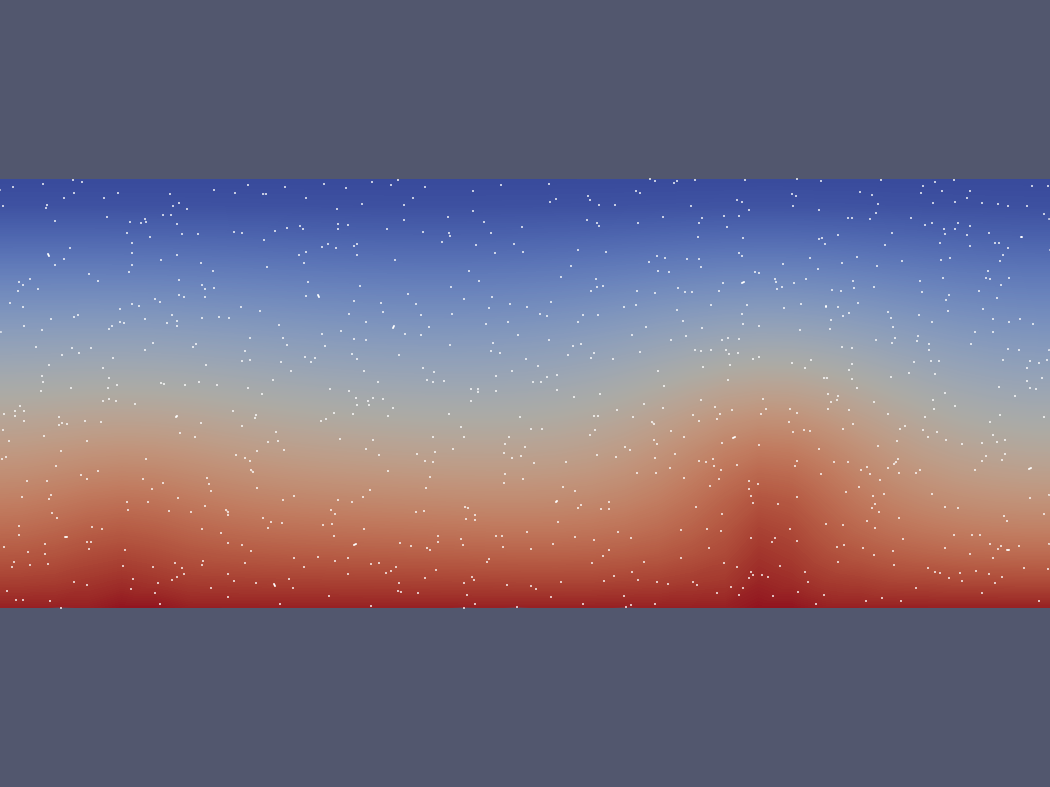
\includegraphics[
                trim={0 180pt 0 180pt}, 
                clip, 
                width=0.38\textwidth
            ]{figures/closed_box/particle_property/677115}
        } & \parbox[c][75pt]{0.38\textwidth}{
            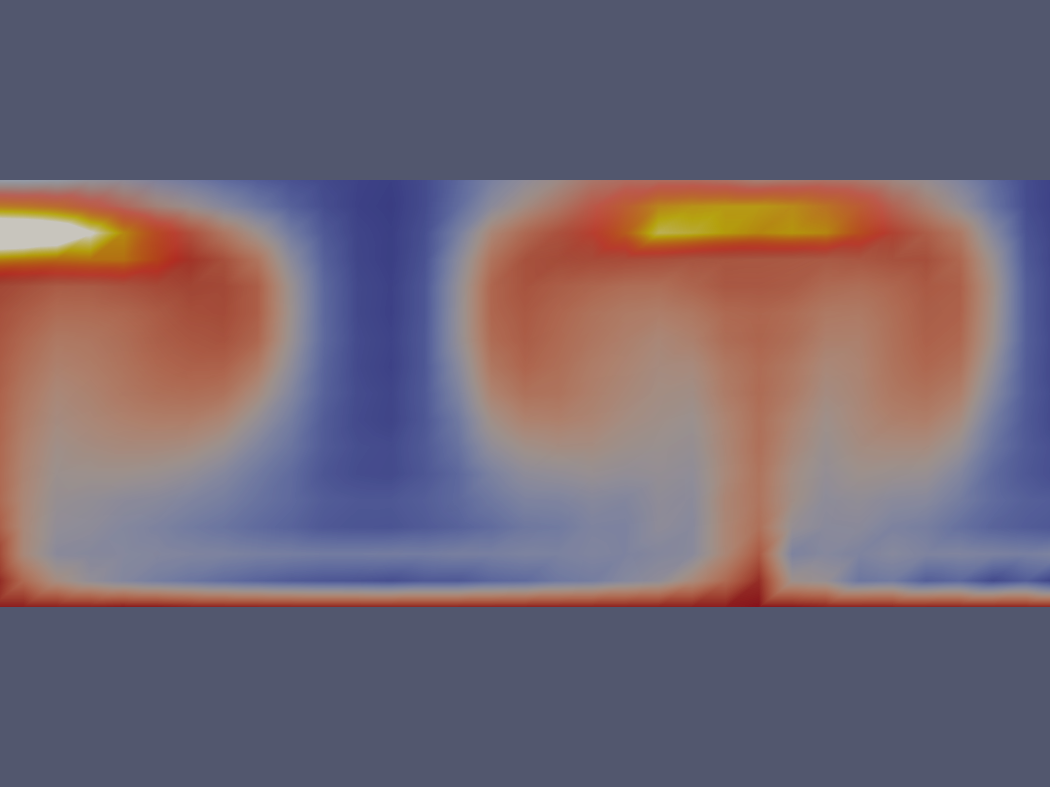
\includegraphics[
                trim={0 180pt 0 180pt}, 
                clip, 
                width=0.38\textwidth
            ]{figures/closed_box/material_model/677115}
        } \\
        \hline
        \num{800992} & \parbox[c][75pt]{0.38\textwidth}{
            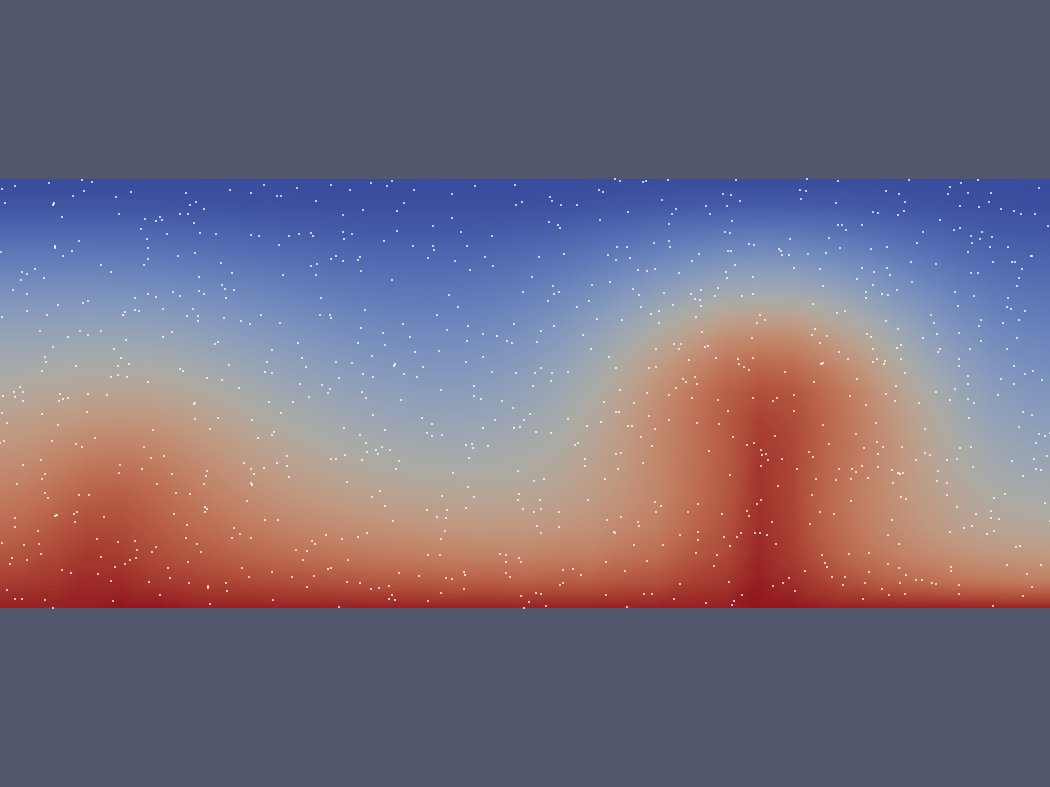
\includegraphics[
                trim={0 180pt 0 180pt}, 
                clip, 
                width=0.38\textwidth
            ]{figures/closed_box/particle_property/800992}
        } & \parbox[c][75pt]{0.38\textwidth}{
            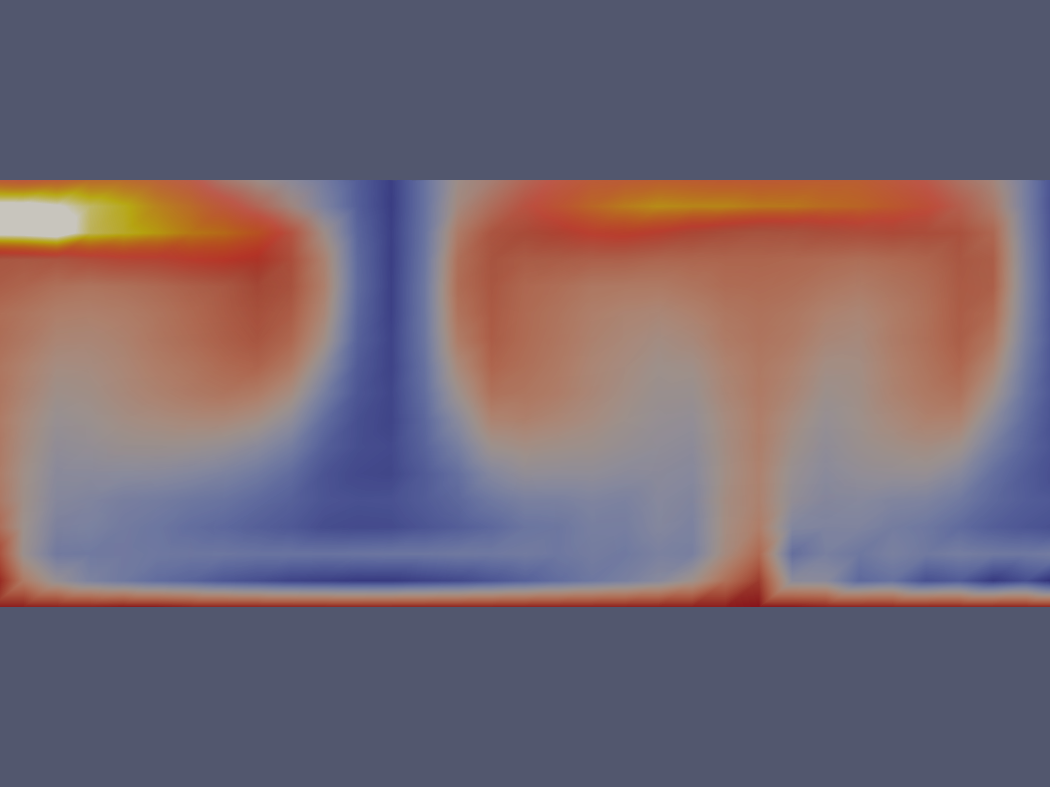
\includegraphics[
                trim={0 180pt 0 180pt}, 
                clip, 
                width=0.38\textwidth
            ]{figures/closed_box/material_model/800992}
        } \\
        \hline
        \num{958796} & \parbox[c][75pt]{0.38\textwidth}{
            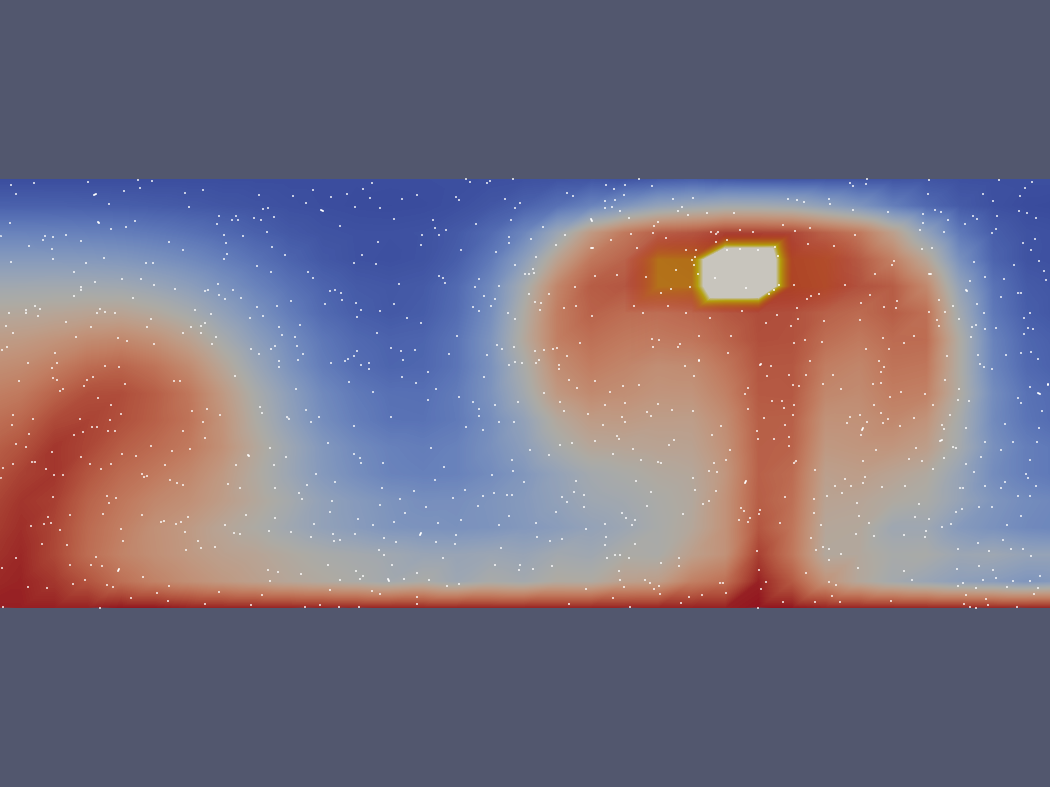
\includegraphics[
                trim={0 180pt 0 180pt}, 
                clip, 
                width=0.38\textwidth
            ]{figures/closed_box/particle_property/958796}
        } & \parbox[c][75pt]{0.38\textwidth}{
            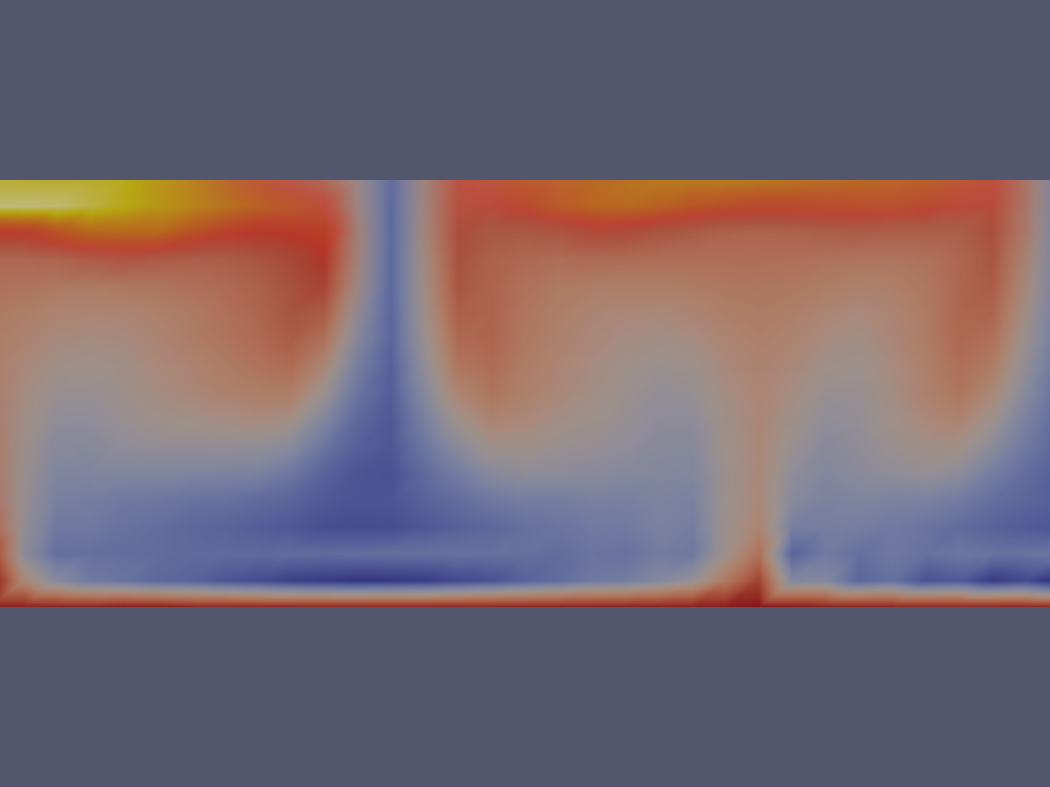
\includegraphics[
                trim={0 180pt 0 180pt}, 
                clip, 
                width=0.38\textwidth
            ]{figures/closed_box/material_model/958796}
        } \\
        \hline
        \num{1.0513e+06} & \parbox[c][75pt]{0.38\textwidth}{
            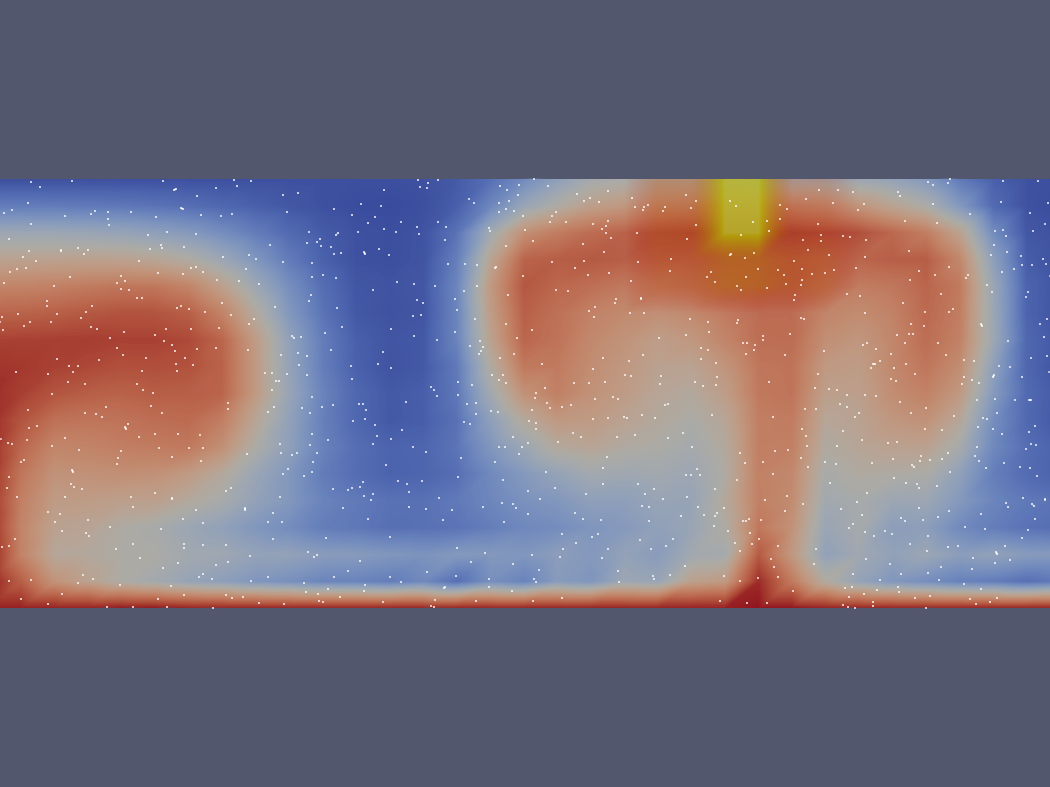
\includegraphics[
                trim={0 180pt 0 180pt}, 
                clip, 
                width=0.38\textwidth
            ]{figures/closed_box/particle_property/1.0513e+06}
        } & \parbox[c][75pt]{0.38\textwidth}{
            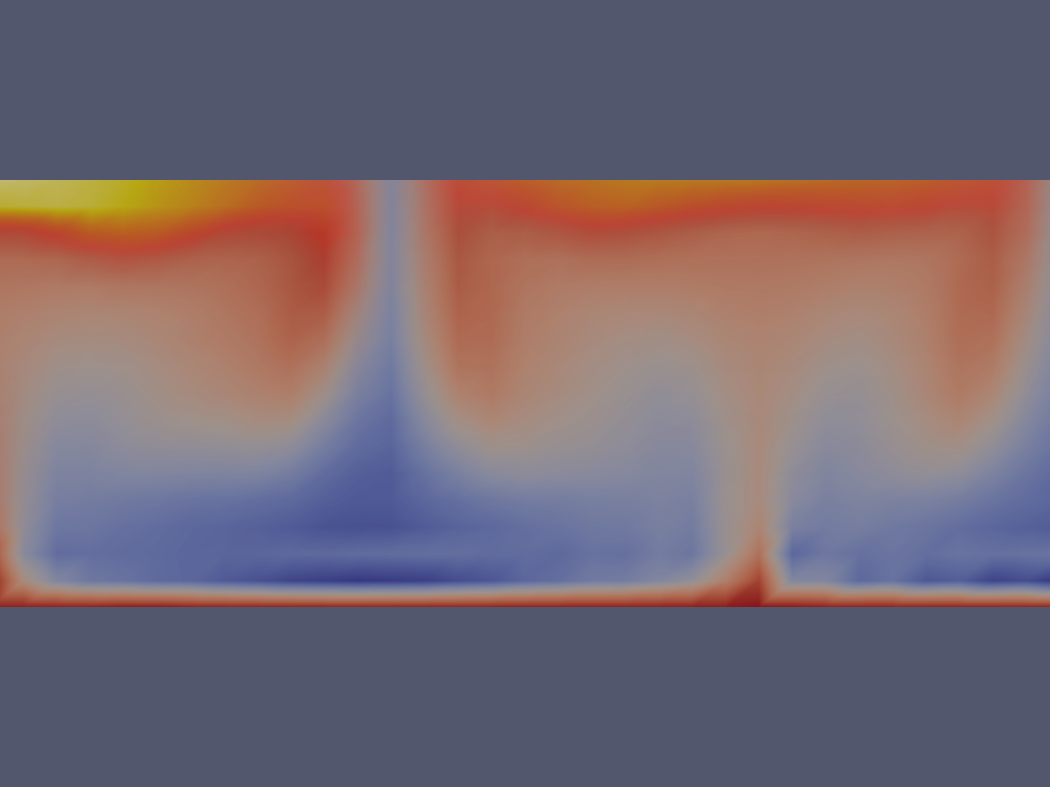
\includegraphics[
                trim={0 180pt 0 180pt}, 
                clip, 
                width=0.38\textwidth
            ]{figures/closed_box/material_model/1.0513e+06}
        } \\
        \hline
        \num{1.28082e+06} & \parbox[c][75pt]{0.38\textwidth}{
            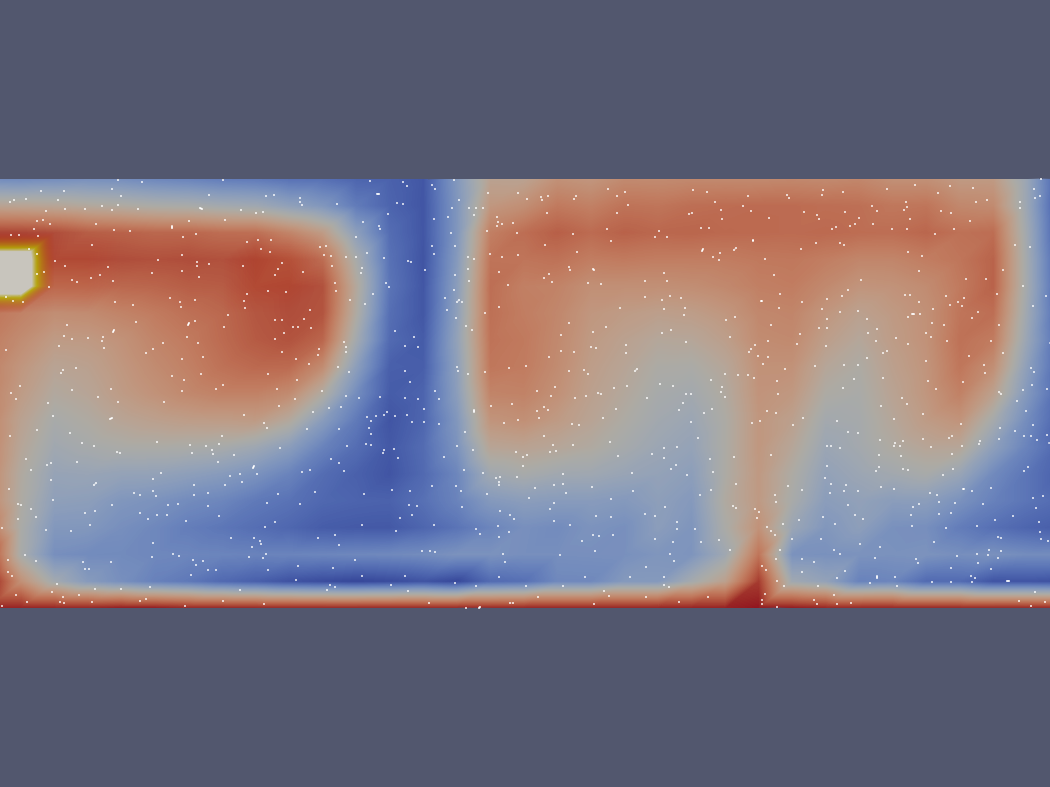
\includegraphics[
                trim={0 180pt 0 180pt}, 
                clip, 
                width=0.38\textwidth
            ]{figures/closed_box/particle_property/1.28082e+06}
        } & \parbox[c][75pt]{0.38\textwidth}{
            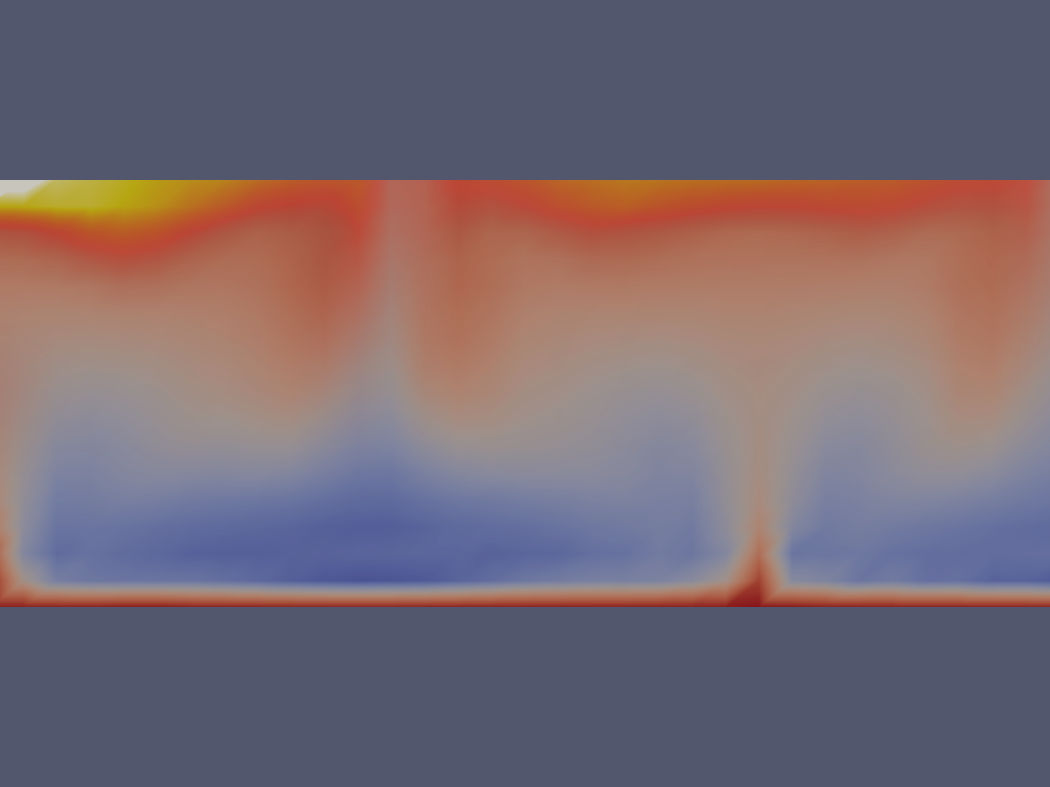
\includegraphics[
                trim={0 180pt 0 180pt}, 
                clip, 
                width=0.38\textwidth
            ]{figures/closed_box/material_model/1.28082e+06}
        }
    \end{tabular}
    \caption{
        Example runs of the closed box model setup with both plugin types.
        \num{2000} particles were used when using the particle property plugin and none were used in the material model one.
        The temperature is represented by the red to blue colour map and the melt is yellow and white.
        Whilst the simulation was run for 3 million years, only the period of \num{600000} years is shown because it shows the principal behaviour.
        Before this the velocities of the particle property plugin are too low to show any dispersion behaviour, and at later times the plumes disperse and the melt disappears.
    }
    \label{fig:closed_box}
\end{figure}

\begin{figure}
    \centering
    \begin{subfigure}{0.49\textwidth}
        \centering
        %% Creator: Matplotlib, PGF backend
%%
%% To include the figure in your LaTeX document, write
%%   \input{<filename>.pgf}
%%
%% Make sure the required packages are loaded in your preamble
%%   \usepackage{pgf}
%%
%% Figures using additional raster images can only be included by \input if
%% they are in the same directory as the main LaTeX file. For loading figures
%% from other directories you can use the `import` package
%%   \usepackage{import}
%% and then include the figures with
%%   \import{<path to file>}{<filename>.pgf}
%%
%% Matplotlib used the following preamble
%%   \usepackage{fontspec}
%%   \setmainfont{DejaVuSerif.ttf}[Path=/home/connor/.local/lib/python3.8/site-packages/matplotlib/mpl-data/fonts/ttf/]
%%   \setsansfont{DejaVuSans.ttf}[Path=/home/connor/.local/lib/python3.8/site-packages/matplotlib/mpl-data/fonts/ttf/]
%%   \setmonofont{DejaVuSansMono.ttf}[Path=/home/connor/.local/lib/python3.8/site-packages/matplotlib/mpl-data/fonts/ttf/]
%%
\begingroup%
\makeatletter%
\begin{pgfpicture}%
\pgfpathrectangle{\pgfpointorigin}{\pgfqpoint{2.853515in}{2.214229in}}%
\pgfusepath{use as bounding box, clip}%
\begin{pgfscope}%
\pgfsetbuttcap%
\pgfsetmiterjoin%
\definecolor{currentfill}{rgb}{1.000000,1.000000,1.000000}%
\pgfsetfillcolor{currentfill}%
\pgfsetlinewidth{0.000000pt}%
\definecolor{currentstroke}{rgb}{1.000000,1.000000,1.000000}%
\pgfsetstrokecolor{currentstroke}%
\pgfsetdash{}{0pt}%
\pgfpathmoveto{\pgfqpoint{0.000000in}{0.000000in}}%
\pgfpathlineto{\pgfqpoint{2.853515in}{0.000000in}}%
\pgfpathlineto{\pgfqpoint{2.853515in}{2.214229in}}%
\pgfpathlineto{\pgfqpoint{0.000000in}{2.214229in}}%
\pgfpathclose%
\pgfusepath{fill}%
\end{pgfscope}%
\begin{pgfscope}%
\pgfsetbuttcap%
\pgfsetmiterjoin%
\definecolor{currentfill}{rgb}{1.000000,1.000000,1.000000}%
\pgfsetfillcolor{currentfill}%
\pgfsetlinewidth{0.000000pt}%
\definecolor{currentstroke}{rgb}{0.000000,0.000000,0.000000}%
\pgfsetstrokecolor{currentstroke}%
\pgfsetstrokeopacity{0.000000}%
\pgfsetdash{}{0pt}%
\pgfpathmoveto{\pgfqpoint{0.478365in}{0.484854in}}%
\pgfpathlineto{\pgfqpoint{2.664972in}{0.484854in}}%
\pgfpathlineto{\pgfqpoint{2.664972in}{2.114229in}}%
\pgfpathlineto{\pgfqpoint{0.478365in}{2.114229in}}%
\pgfpathclose%
\pgfusepath{fill}%
\end{pgfscope}%
\begin{pgfscope}%
\pgfpathrectangle{\pgfqpoint{0.478365in}{0.484854in}}{\pgfqpoint{2.186607in}{1.629375in}}%
\pgfusepath{clip}%
\pgfsetbuttcap%
\pgfsetroundjoin%
\definecolor{currentfill}{rgb}{0.121569,0.466667,0.705882}%
\pgfsetfillcolor{currentfill}%
\pgfsetlinewidth{0.000000pt}%
\definecolor{currentstroke}{rgb}{0.000000,0.000000,0.000000}%
\pgfsetstrokecolor{currentstroke}%
\pgfsetdash{}{0pt}%
\pgfpathmoveto{\pgfqpoint{-0.979373in}{0.484854in}}%
\pgfpathlineto{\pgfqpoint{-0.979373in}{0.484854in}}%
\pgfpathlineto{\pgfqpoint{-0.933818in}{0.484854in}}%
\pgfpathlineto{\pgfqpoint{-0.897375in}{0.484854in}}%
\pgfpathlineto{\pgfqpoint{-0.860931in}{0.484854in}}%
\pgfpathlineto{\pgfqpoint{-0.824488in}{0.484854in}}%
\pgfpathlineto{\pgfqpoint{-0.788045in}{0.484854in}}%
\pgfpathlineto{\pgfqpoint{-0.751601in}{0.484854in}}%
\pgfpathlineto{\pgfqpoint{-0.715158in}{0.484854in}}%
\pgfpathlineto{\pgfqpoint{-0.678714in}{0.484854in}}%
\pgfpathlineto{\pgfqpoint{-0.642271in}{0.484854in}}%
\pgfpathlineto{\pgfqpoint{-0.605827in}{0.484854in}}%
\pgfpathlineto{\pgfqpoint{-0.569384in}{0.484854in}}%
\pgfpathlineto{\pgfqpoint{-0.532940in}{0.484854in}}%
\pgfpathlineto{\pgfqpoint{-0.496497in}{0.484854in}}%
\pgfpathlineto{\pgfqpoint{-0.460054in}{0.484854in}}%
\pgfpathlineto{\pgfqpoint{-0.423610in}{0.484854in}}%
\pgfpathlineto{\pgfqpoint{-0.387167in}{0.484854in}}%
\pgfpathlineto{\pgfqpoint{-0.350723in}{0.484854in}}%
\pgfpathlineto{\pgfqpoint{-0.314280in}{0.484854in}}%
\pgfpathlineto{\pgfqpoint{-0.277836in}{0.484854in}}%
\pgfpathlineto{\pgfqpoint{-0.241393in}{0.484854in}}%
\pgfpathlineto{\pgfqpoint{-0.204949in}{0.484854in}}%
\pgfpathlineto{\pgfqpoint{-0.168506in}{0.484854in}}%
\pgfpathlineto{\pgfqpoint{-0.132062in}{0.484854in}}%
\pgfpathlineto{\pgfqpoint{-0.095619in}{0.484854in}}%
\pgfpathlineto{\pgfqpoint{-0.059176in}{0.484854in}}%
\pgfpathlineto{\pgfqpoint{-0.022732in}{0.484854in}}%
\pgfpathlineto{\pgfqpoint{0.013711in}{0.484854in}}%
\pgfpathlineto{\pgfqpoint{0.050155in}{0.484854in}}%
\pgfpathlineto{\pgfqpoint{0.086598in}{0.484854in}}%
\pgfpathlineto{\pgfqpoint{0.123042in}{0.484854in}}%
\pgfpathlineto{\pgfqpoint{0.159485in}{0.484854in}}%
\pgfpathlineto{\pgfqpoint{0.195929in}{0.484854in}}%
\pgfpathlineto{\pgfqpoint{0.232372in}{0.484854in}}%
\pgfpathlineto{\pgfqpoint{0.268815in}{0.484854in}}%
\pgfpathlineto{\pgfqpoint{0.305259in}{0.484854in}}%
\pgfpathlineto{\pgfqpoint{0.341702in}{0.484854in}}%
\pgfpathlineto{\pgfqpoint{0.378146in}{0.484854in}}%
\pgfpathlineto{\pgfqpoint{0.414589in}{0.484854in}}%
\pgfpathlineto{\pgfqpoint{0.451033in}{0.484854in}}%
\pgfpathlineto{\pgfqpoint{0.487476in}{0.484854in}}%
\pgfpathlineto{\pgfqpoint{0.523920in}{0.484854in}}%
\pgfpathlineto{\pgfqpoint{0.560363in}{0.484854in}}%
\pgfpathlineto{\pgfqpoint{0.596806in}{0.484854in}}%
\pgfpathlineto{\pgfqpoint{0.633250in}{0.484854in}}%
\pgfpathlineto{\pgfqpoint{0.669693in}{0.484854in}}%
\pgfpathlineto{\pgfqpoint{0.706137in}{0.484854in}}%
\pgfpathlineto{\pgfqpoint{0.742580in}{0.484854in}}%
\pgfpathlineto{\pgfqpoint{0.779024in}{0.484854in}}%
\pgfpathlineto{\pgfqpoint{0.815467in}{0.484854in}}%
\pgfpathlineto{\pgfqpoint{0.851911in}{0.484854in}}%
\pgfpathlineto{\pgfqpoint{0.888354in}{0.484854in}}%
\pgfpathlineto{\pgfqpoint{0.924798in}{0.484854in}}%
\pgfpathlineto{\pgfqpoint{0.961241in}{0.484854in}}%
\pgfpathlineto{\pgfqpoint{0.997684in}{0.484854in}}%
\pgfpathlineto{\pgfqpoint{1.034128in}{0.484854in}}%
\pgfpathlineto{\pgfqpoint{1.070571in}{0.484854in}}%
\pgfpathlineto{\pgfqpoint{1.107015in}{0.484854in}}%
\pgfpathlineto{\pgfqpoint{1.143458in}{0.484854in}}%
\pgfpathlineto{\pgfqpoint{1.179902in}{0.484854in}}%
\pgfpathlineto{\pgfqpoint{1.216345in}{0.484854in}}%
\pgfpathlineto{\pgfqpoint{1.252789in}{0.484854in}}%
\pgfpathlineto{\pgfqpoint{1.289232in}{0.484854in}}%
\pgfpathlineto{\pgfqpoint{1.325675in}{0.484854in}}%
\pgfpathlineto{\pgfqpoint{1.362119in}{0.484854in}}%
\pgfpathlineto{\pgfqpoint{1.398562in}{0.484854in}}%
\pgfpathlineto{\pgfqpoint{1.435006in}{0.484854in}}%
\pgfpathlineto{\pgfqpoint{1.471449in}{0.484854in}}%
\pgfpathlineto{\pgfqpoint{1.507893in}{0.484854in}}%
\pgfpathlineto{\pgfqpoint{1.544336in}{0.484854in}}%
\pgfpathlineto{\pgfqpoint{1.580780in}{0.484854in}}%
\pgfpathlineto{\pgfqpoint{1.617223in}{0.484854in}}%
\pgfpathlineto{\pgfqpoint{1.653666in}{0.484854in}}%
\pgfpathlineto{\pgfqpoint{1.690110in}{0.484854in}}%
\pgfpathlineto{\pgfqpoint{1.726553in}{0.484854in}}%
\pgfpathlineto{\pgfqpoint{1.762997in}{0.484854in}}%
\pgfpathlineto{\pgfqpoint{1.799440in}{0.484854in}}%
\pgfpathlineto{\pgfqpoint{1.835884in}{0.484854in}}%
\pgfpathlineto{\pgfqpoint{1.872327in}{0.484854in}}%
\pgfpathlineto{\pgfqpoint{1.908771in}{0.484854in}}%
\pgfpathlineto{\pgfqpoint{1.945214in}{0.484854in}}%
\pgfpathlineto{\pgfqpoint{1.981658in}{0.484854in}}%
\pgfpathlineto{\pgfqpoint{2.018101in}{0.484854in}}%
\pgfpathlineto{\pgfqpoint{2.054544in}{0.484854in}}%
\pgfpathlineto{\pgfqpoint{2.090988in}{0.484854in}}%
\pgfpathlineto{\pgfqpoint{2.127431in}{0.484854in}}%
\pgfpathlineto{\pgfqpoint{2.163875in}{0.484854in}}%
\pgfpathlineto{\pgfqpoint{2.200318in}{0.484854in}}%
\pgfpathlineto{\pgfqpoint{2.236762in}{0.484854in}}%
\pgfpathlineto{\pgfqpoint{2.273205in}{0.484854in}}%
\pgfpathlineto{\pgfqpoint{2.309649in}{0.484854in}}%
\pgfpathlineto{\pgfqpoint{2.346092in}{0.484854in}}%
\pgfpathlineto{\pgfqpoint{2.382535in}{0.484854in}}%
\pgfpathlineto{\pgfqpoint{2.418979in}{0.484854in}}%
\pgfpathlineto{\pgfqpoint{2.455422in}{0.484854in}}%
\pgfpathlineto{\pgfqpoint{2.491866in}{0.484854in}}%
\pgfpathlineto{\pgfqpoint{2.528309in}{0.484854in}}%
\pgfpathlineto{\pgfqpoint{2.564753in}{0.484854in}}%
\pgfpathlineto{\pgfqpoint{2.601196in}{0.484854in}}%
\pgfpathlineto{\pgfqpoint{2.637640in}{0.484854in}}%
\pgfpathlineto{\pgfqpoint{2.664972in}{0.484854in}}%
\pgfpathlineto{\pgfqpoint{2.664972in}{0.636214in}}%
\pgfpathlineto{\pgfqpoint{2.664972in}{0.636214in}}%
\pgfpathlineto{\pgfqpoint{2.637640in}{0.636153in}}%
\pgfpathlineto{\pgfqpoint{2.601196in}{0.636075in}}%
\pgfpathlineto{\pgfqpoint{2.564753in}{0.636003in}}%
\pgfpathlineto{\pgfqpoint{2.528309in}{0.635925in}}%
\pgfpathlineto{\pgfqpoint{2.491866in}{0.636197in}}%
\pgfpathlineto{\pgfqpoint{2.455422in}{0.636119in}}%
\pgfpathlineto{\pgfqpoint{2.418979in}{0.636045in}}%
\pgfpathlineto{\pgfqpoint{2.382535in}{0.635354in}}%
\pgfpathlineto{\pgfqpoint{2.346092in}{0.635296in}}%
\pgfpathlineto{\pgfqpoint{2.309649in}{0.635181in}}%
\pgfpathlineto{\pgfqpoint{2.273205in}{0.635087in}}%
\pgfpathlineto{\pgfqpoint{2.236762in}{0.634250in}}%
\pgfpathlineto{\pgfqpoint{2.200318in}{0.632029in}}%
\pgfpathlineto{\pgfqpoint{2.163875in}{0.628624in}}%
\pgfpathlineto{\pgfqpoint{2.127431in}{0.627851in}}%
\pgfpathlineto{\pgfqpoint{2.090988in}{0.625985in}}%
\pgfpathlineto{\pgfqpoint{2.054544in}{0.625046in}}%
\pgfpathlineto{\pgfqpoint{2.018101in}{0.623343in}}%
\pgfpathlineto{\pgfqpoint{1.981658in}{0.620584in}}%
\pgfpathlineto{\pgfqpoint{1.945214in}{0.618823in}}%
\pgfpathlineto{\pgfqpoint{1.908771in}{0.616853in}}%
\pgfpathlineto{\pgfqpoint{1.872327in}{0.614922in}}%
\pgfpathlineto{\pgfqpoint{1.835884in}{0.611718in}}%
\pgfpathlineto{\pgfqpoint{1.799440in}{0.609729in}}%
\pgfpathlineto{\pgfqpoint{1.762997in}{0.607249in}}%
\pgfpathlineto{\pgfqpoint{1.726553in}{0.601246in}}%
\pgfpathlineto{\pgfqpoint{1.690110in}{0.599151in}}%
\pgfpathlineto{\pgfqpoint{1.653666in}{0.596882in}}%
\pgfpathlineto{\pgfqpoint{1.617223in}{0.593614in}}%
\pgfpathlineto{\pgfqpoint{1.580780in}{0.591104in}}%
\pgfpathlineto{\pgfqpoint{1.544336in}{0.588385in}}%
\pgfpathlineto{\pgfqpoint{1.507893in}{0.585337in}}%
\pgfpathlineto{\pgfqpoint{1.471449in}{0.580960in}}%
\pgfpathlineto{\pgfqpoint{1.435006in}{0.569059in}}%
\pgfpathlineto{\pgfqpoint{1.398562in}{0.567746in}}%
\pgfpathlineto{\pgfqpoint{1.362119in}{0.567143in}}%
\pgfpathlineto{\pgfqpoint{1.325675in}{0.563374in}}%
\pgfpathlineto{\pgfqpoint{1.289232in}{0.558673in}}%
\pgfpathlineto{\pgfqpoint{1.252789in}{0.553179in}}%
\pgfpathlineto{\pgfqpoint{1.216345in}{0.546783in}}%
\pgfpathlineto{\pgfqpoint{1.179902in}{0.541475in}}%
\pgfpathlineto{\pgfqpoint{1.143458in}{0.534812in}}%
\pgfpathlineto{\pgfqpoint{1.107015in}{0.528068in}}%
\pgfpathlineto{\pgfqpoint{1.070571in}{0.520275in}}%
\pgfpathlineto{\pgfqpoint{1.034128in}{0.511484in}}%
\pgfpathlineto{\pgfqpoint{0.997684in}{0.502707in}}%
\pgfpathlineto{\pgfqpoint{0.961241in}{0.492974in}}%
\pgfpathlineto{\pgfqpoint{0.924798in}{0.484854in}}%
\pgfpathlineto{\pgfqpoint{0.888354in}{0.484854in}}%
\pgfpathlineto{\pgfqpoint{0.851911in}{0.484854in}}%
\pgfpathlineto{\pgfqpoint{0.815467in}{0.484854in}}%
\pgfpathlineto{\pgfqpoint{0.779024in}{0.484854in}}%
\pgfpathlineto{\pgfqpoint{0.742580in}{0.484854in}}%
\pgfpathlineto{\pgfqpoint{0.706137in}{0.484854in}}%
\pgfpathlineto{\pgfqpoint{0.669693in}{0.484854in}}%
\pgfpathlineto{\pgfqpoint{0.633250in}{0.484854in}}%
\pgfpathlineto{\pgfqpoint{0.596806in}{0.484854in}}%
\pgfpathlineto{\pgfqpoint{0.560363in}{0.484854in}}%
\pgfpathlineto{\pgfqpoint{0.523920in}{0.484854in}}%
\pgfpathlineto{\pgfqpoint{0.487476in}{0.484854in}}%
\pgfpathlineto{\pgfqpoint{0.451033in}{0.484854in}}%
\pgfpathlineto{\pgfqpoint{0.414589in}{0.484854in}}%
\pgfpathlineto{\pgfqpoint{0.378146in}{0.484854in}}%
\pgfpathlineto{\pgfqpoint{0.341702in}{0.484854in}}%
\pgfpathlineto{\pgfqpoint{0.305259in}{0.484854in}}%
\pgfpathlineto{\pgfqpoint{0.268815in}{0.484854in}}%
\pgfpathlineto{\pgfqpoint{0.232372in}{0.484854in}}%
\pgfpathlineto{\pgfqpoint{0.195929in}{0.484854in}}%
\pgfpathlineto{\pgfqpoint{0.159485in}{0.484854in}}%
\pgfpathlineto{\pgfqpoint{0.123042in}{0.484854in}}%
\pgfpathlineto{\pgfqpoint{0.086598in}{0.484854in}}%
\pgfpathlineto{\pgfqpoint{0.050155in}{0.484854in}}%
\pgfpathlineto{\pgfqpoint{0.013711in}{0.484854in}}%
\pgfpathlineto{\pgfqpoint{-0.022732in}{0.484854in}}%
\pgfpathlineto{\pgfqpoint{-0.059176in}{0.484854in}}%
\pgfpathlineto{\pgfqpoint{-0.095619in}{0.484854in}}%
\pgfpathlineto{\pgfqpoint{-0.132062in}{0.484854in}}%
\pgfpathlineto{\pgfqpoint{-0.168506in}{0.484854in}}%
\pgfpathlineto{\pgfqpoint{-0.204949in}{0.484854in}}%
\pgfpathlineto{\pgfqpoint{-0.241393in}{0.484854in}}%
\pgfpathlineto{\pgfqpoint{-0.277836in}{0.484854in}}%
\pgfpathlineto{\pgfqpoint{-0.314280in}{0.484854in}}%
\pgfpathlineto{\pgfqpoint{-0.350723in}{0.484854in}}%
\pgfpathlineto{\pgfqpoint{-0.387167in}{0.484854in}}%
\pgfpathlineto{\pgfqpoint{-0.423610in}{0.484854in}}%
\pgfpathlineto{\pgfqpoint{-0.460054in}{0.484854in}}%
\pgfpathlineto{\pgfqpoint{-0.496497in}{0.484854in}}%
\pgfpathlineto{\pgfqpoint{-0.532940in}{0.484854in}}%
\pgfpathlineto{\pgfqpoint{-0.569384in}{0.484854in}}%
\pgfpathlineto{\pgfqpoint{-0.605827in}{0.484854in}}%
\pgfpathlineto{\pgfqpoint{-0.642271in}{0.484854in}}%
\pgfpathlineto{\pgfqpoint{-0.678714in}{0.484854in}}%
\pgfpathlineto{\pgfqpoint{-0.715158in}{0.484854in}}%
\pgfpathlineto{\pgfqpoint{-0.751601in}{0.484854in}}%
\pgfpathlineto{\pgfqpoint{-0.788045in}{0.484854in}}%
\pgfpathlineto{\pgfqpoint{-0.824488in}{0.484854in}}%
\pgfpathlineto{\pgfqpoint{-0.860931in}{0.484854in}}%
\pgfpathlineto{\pgfqpoint{-0.897375in}{0.484854in}}%
\pgfpathlineto{\pgfqpoint{-0.933818in}{0.484854in}}%
\pgfpathlineto{\pgfqpoint{-0.979373in}{0.484854in}}%
\pgfpathclose%
\pgfusepath{fill}%
\end{pgfscope}%
\begin{pgfscope}%
\pgfpathrectangle{\pgfqpoint{0.478365in}{0.484854in}}{\pgfqpoint{2.186607in}{1.629375in}}%
\pgfusepath{clip}%
\pgfsetbuttcap%
\pgfsetroundjoin%
\definecolor{currentfill}{rgb}{1.000000,0.498039,0.054902}%
\pgfsetfillcolor{currentfill}%
\pgfsetlinewidth{0.000000pt}%
\definecolor{currentstroke}{rgb}{0.000000,0.000000,0.000000}%
\pgfsetstrokecolor{currentstroke}%
\pgfsetdash{}{0pt}%
\pgfpathmoveto{\pgfqpoint{-0.979373in}{0.484854in}}%
\pgfpathlineto{\pgfqpoint{-0.979373in}{0.484854in}}%
\pgfpathlineto{\pgfqpoint{-0.933818in}{0.484854in}}%
\pgfpathlineto{\pgfqpoint{-0.897375in}{0.484854in}}%
\pgfpathlineto{\pgfqpoint{-0.860931in}{0.484854in}}%
\pgfpathlineto{\pgfqpoint{-0.824488in}{0.484854in}}%
\pgfpathlineto{\pgfqpoint{-0.788045in}{0.484854in}}%
\pgfpathlineto{\pgfqpoint{-0.751601in}{0.484854in}}%
\pgfpathlineto{\pgfqpoint{-0.715158in}{0.484854in}}%
\pgfpathlineto{\pgfqpoint{-0.678714in}{0.484854in}}%
\pgfpathlineto{\pgfqpoint{-0.642271in}{0.484854in}}%
\pgfpathlineto{\pgfqpoint{-0.605827in}{0.484854in}}%
\pgfpathlineto{\pgfqpoint{-0.569384in}{0.484854in}}%
\pgfpathlineto{\pgfqpoint{-0.532940in}{0.484854in}}%
\pgfpathlineto{\pgfqpoint{-0.496497in}{0.484854in}}%
\pgfpathlineto{\pgfqpoint{-0.460054in}{0.484854in}}%
\pgfpathlineto{\pgfqpoint{-0.423610in}{0.484854in}}%
\pgfpathlineto{\pgfqpoint{-0.387167in}{0.484854in}}%
\pgfpathlineto{\pgfqpoint{-0.350723in}{0.484854in}}%
\pgfpathlineto{\pgfqpoint{-0.314280in}{0.484854in}}%
\pgfpathlineto{\pgfqpoint{-0.277836in}{0.484854in}}%
\pgfpathlineto{\pgfqpoint{-0.241393in}{0.484854in}}%
\pgfpathlineto{\pgfqpoint{-0.204949in}{0.484854in}}%
\pgfpathlineto{\pgfqpoint{-0.168506in}{0.484854in}}%
\pgfpathlineto{\pgfqpoint{-0.132062in}{0.484854in}}%
\pgfpathlineto{\pgfqpoint{-0.095619in}{0.484854in}}%
\pgfpathlineto{\pgfqpoint{-0.059176in}{0.484854in}}%
\pgfpathlineto{\pgfqpoint{-0.022732in}{0.484854in}}%
\pgfpathlineto{\pgfqpoint{0.013711in}{0.484854in}}%
\pgfpathlineto{\pgfqpoint{0.050155in}{0.484854in}}%
\pgfpathlineto{\pgfqpoint{0.086598in}{0.484854in}}%
\pgfpathlineto{\pgfqpoint{0.123042in}{0.484854in}}%
\pgfpathlineto{\pgfqpoint{0.159485in}{0.484854in}}%
\pgfpathlineto{\pgfqpoint{0.195929in}{0.484854in}}%
\pgfpathlineto{\pgfqpoint{0.232372in}{0.484854in}}%
\pgfpathlineto{\pgfqpoint{0.268815in}{0.484854in}}%
\pgfpathlineto{\pgfqpoint{0.305259in}{0.484854in}}%
\pgfpathlineto{\pgfqpoint{0.341702in}{0.484854in}}%
\pgfpathlineto{\pgfqpoint{0.378146in}{0.484854in}}%
\pgfpathlineto{\pgfqpoint{0.414589in}{0.484854in}}%
\pgfpathlineto{\pgfqpoint{0.451033in}{0.484854in}}%
\pgfpathlineto{\pgfqpoint{0.487476in}{0.484854in}}%
\pgfpathlineto{\pgfqpoint{0.523920in}{0.484854in}}%
\pgfpathlineto{\pgfqpoint{0.560363in}{0.484854in}}%
\pgfpathlineto{\pgfqpoint{0.596806in}{0.484854in}}%
\pgfpathlineto{\pgfqpoint{0.633250in}{0.484854in}}%
\pgfpathlineto{\pgfqpoint{0.669693in}{0.484854in}}%
\pgfpathlineto{\pgfqpoint{0.706137in}{0.484854in}}%
\pgfpathlineto{\pgfqpoint{0.742580in}{0.484854in}}%
\pgfpathlineto{\pgfqpoint{0.779024in}{0.484854in}}%
\pgfpathlineto{\pgfqpoint{0.815467in}{0.484854in}}%
\pgfpathlineto{\pgfqpoint{0.851911in}{0.484854in}}%
\pgfpathlineto{\pgfqpoint{0.888354in}{0.484854in}}%
\pgfpathlineto{\pgfqpoint{0.924798in}{0.484854in}}%
\pgfpathlineto{\pgfqpoint{0.961241in}{0.492974in}}%
\pgfpathlineto{\pgfqpoint{0.997684in}{0.502707in}}%
\pgfpathlineto{\pgfqpoint{1.034128in}{0.511484in}}%
\pgfpathlineto{\pgfqpoint{1.070571in}{0.520275in}}%
\pgfpathlineto{\pgfqpoint{1.107015in}{0.528068in}}%
\pgfpathlineto{\pgfqpoint{1.143458in}{0.534812in}}%
\pgfpathlineto{\pgfqpoint{1.179902in}{0.541475in}}%
\pgfpathlineto{\pgfqpoint{1.216345in}{0.546783in}}%
\pgfpathlineto{\pgfqpoint{1.252789in}{0.553179in}}%
\pgfpathlineto{\pgfqpoint{1.289232in}{0.558673in}}%
\pgfpathlineto{\pgfqpoint{1.325675in}{0.563374in}}%
\pgfpathlineto{\pgfqpoint{1.362119in}{0.567143in}}%
\pgfpathlineto{\pgfqpoint{1.398562in}{0.567746in}}%
\pgfpathlineto{\pgfqpoint{1.435006in}{0.569059in}}%
\pgfpathlineto{\pgfqpoint{1.471449in}{0.580960in}}%
\pgfpathlineto{\pgfqpoint{1.507893in}{0.585337in}}%
\pgfpathlineto{\pgfqpoint{1.544336in}{0.588385in}}%
\pgfpathlineto{\pgfqpoint{1.580780in}{0.591104in}}%
\pgfpathlineto{\pgfqpoint{1.617223in}{0.593614in}}%
\pgfpathlineto{\pgfqpoint{1.653666in}{0.596882in}}%
\pgfpathlineto{\pgfqpoint{1.690110in}{0.599151in}}%
\pgfpathlineto{\pgfqpoint{1.726553in}{0.601246in}}%
\pgfpathlineto{\pgfqpoint{1.762997in}{0.607249in}}%
\pgfpathlineto{\pgfqpoint{1.799440in}{0.609729in}}%
\pgfpathlineto{\pgfqpoint{1.835884in}{0.611718in}}%
\pgfpathlineto{\pgfqpoint{1.872327in}{0.614922in}}%
\pgfpathlineto{\pgfqpoint{1.908771in}{0.616853in}}%
\pgfpathlineto{\pgfqpoint{1.945214in}{0.618823in}}%
\pgfpathlineto{\pgfqpoint{1.981658in}{0.620584in}}%
\pgfpathlineto{\pgfqpoint{2.018101in}{0.623343in}}%
\pgfpathlineto{\pgfqpoint{2.054544in}{0.625046in}}%
\pgfpathlineto{\pgfqpoint{2.090988in}{0.625985in}}%
\pgfpathlineto{\pgfqpoint{2.127431in}{0.627851in}}%
\pgfpathlineto{\pgfqpoint{2.163875in}{0.628624in}}%
\pgfpathlineto{\pgfqpoint{2.200318in}{0.632029in}}%
\pgfpathlineto{\pgfqpoint{2.236762in}{0.634250in}}%
\pgfpathlineto{\pgfqpoint{2.273205in}{0.635087in}}%
\pgfpathlineto{\pgfqpoint{2.309649in}{0.635181in}}%
\pgfpathlineto{\pgfqpoint{2.346092in}{0.635296in}}%
\pgfpathlineto{\pgfqpoint{2.382535in}{0.635354in}}%
\pgfpathlineto{\pgfqpoint{2.418979in}{0.636045in}}%
\pgfpathlineto{\pgfqpoint{2.455422in}{0.636119in}}%
\pgfpathlineto{\pgfqpoint{2.491866in}{0.636197in}}%
\pgfpathlineto{\pgfqpoint{2.528309in}{0.635925in}}%
\pgfpathlineto{\pgfqpoint{2.564753in}{0.636003in}}%
\pgfpathlineto{\pgfqpoint{2.601196in}{0.636075in}}%
\pgfpathlineto{\pgfqpoint{2.637640in}{0.636153in}}%
\pgfpathlineto{\pgfqpoint{2.664972in}{0.636214in}}%
\pgfpathlineto{\pgfqpoint{2.664972in}{0.759668in}}%
\pgfpathlineto{\pgfqpoint{2.664972in}{0.759668in}}%
\pgfpathlineto{\pgfqpoint{2.637640in}{0.759498in}}%
\pgfpathlineto{\pgfqpoint{2.601196in}{0.759357in}}%
\pgfpathlineto{\pgfqpoint{2.564753in}{0.758723in}}%
\pgfpathlineto{\pgfqpoint{2.528309in}{0.758581in}}%
\pgfpathlineto{\pgfqpoint{2.491866in}{0.756452in}}%
\pgfpathlineto{\pgfqpoint{2.455422in}{0.756311in}}%
\pgfpathlineto{\pgfqpoint{2.418979in}{0.756178in}}%
\pgfpathlineto{\pgfqpoint{2.382535in}{0.756983in}}%
\pgfpathlineto{\pgfqpoint{2.346092in}{0.755980in}}%
\pgfpathlineto{\pgfqpoint{2.309649in}{0.755891in}}%
\pgfpathlineto{\pgfqpoint{2.273205in}{0.754856in}}%
\pgfpathlineto{\pgfqpoint{2.236762in}{0.752957in}}%
\pgfpathlineto{\pgfqpoint{2.200318in}{0.748000in}}%
\pgfpathlineto{\pgfqpoint{2.163875in}{0.735387in}}%
\pgfpathlineto{\pgfqpoint{2.127431in}{0.734039in}}%
\pgfpathlineto{\pgfqpoint{2.090988in}{0.731667in}}%
\pgfpathlineto{\pgfqpoint{2.054544in}{0.730630in}}%
\pgfpathlineto{\pgfqpoint{2.018101in}{0.726462in}}%
\pgfpathlineto{\pgfqpoint{1.981658in}{0.720942in}}%
\pgfpathlineto{\pgfqpoint{1.945214in}{0.716412in}}%
\pgfpathlineto{\pgfqpoint{1.908771in}{0.712496in}}%
\pgfpathlineto{\pgfqpoint{1.872327in}{0.708828in}}%
\pgfpathlineto{\pgfqpoint{1.835884in}{0.702724in}}%
\pgfpathlineto{\pgfqpoint{1.799440in}{0.698293in}}%
\pgfpathlineto{\pgfqpoint{1.762997in}{0.693311in}}%
\pgfpathlineto{\pgfqpoint{1.726553in}{0.676923in}}%
\pgfpathlineto{\pgfqpoint{1.690110in}{0.674060in}}%
\pgfpathlineto{\pgfqpoint{1.653666in}{0.670888in}}%
\pgfpathlineto{\pgfqpoint{1.617223in}{0.666026in}}%
\pgfpathlineto{\pgfqpoint{1.580780in}{0.662398in}}%
\pgfpathlineto{\pgfqpoint{1.544336in}{0.658392in}}%
\pgfpathlineto{\pgfqpoint{1.507893in}{0.653541in}}%
\pgfpathlineto{\pgfqpoint{1.471449in}{0.645441in}}%
\pgfpathlineto{\pgfqpoint{1.435006in}{0.626052in}}%
\pgfpathlineto{\pgfqpoint{1.398562in}{0.622801in}}%
\pgfpathlineto{\pgfqpoint{1.362119in}{0.622071in}}%
\pgfpathlineto{\pgfqpoint{1.325675in}{0.615269in}}%
\pgfpathlineto{\pgfqpoint{1.289232in}{0.607464in}}%
\pgfpathlineto{\pgfqpoint{1.252789in}{0.598673in}}%
\pgfpathlineto{\pgfqpoint{1.216345in}{0.587621in}}%
\pgfpathlineto{\pgfqpoint{1.179902in}{0.578816in}}%
\pgfpathlineto{\pgfqpoint{1.143458in}{0.567762in}}%
\pgfpathlineto{\pgfqpoint{1.107015in}{0.556572in}}%
\pgfpathlineto{\pgfqpoint{1.070571in}{0.543834in}}%
\pgfpathlineto{\pgfqpoint{1.034128in}{0.529217in}}%
\pgfpathlineto{\pgfqpoint{0.997684in}{0.514692in}}%
\pgfpathlineto{\pgfqpoint{0.961241in}{0.498468in}}%
\pgfpathlineto{\pgfqpoint{0.924798in}{0.484854in}}%
\pgfpathlineto{\pgfqpoint{0.888354in}{0.484854in}}%
\pgfpathlineto{\pgfqpoint{0.851911in}{0.484854in}}%
\pgfpathlineto{\pgfqpoint{0.815467in}{0.484854in}}%
\pgfpathlineto{\pgfqpoint{0.779024in}{0.484854in}}%
\pgfpathlineto{\pgfqpoint{0.742580in}{0.484854in}}%
\pgfpathlineto{\pgfqpoint{0.706137in}{0.484854in}}%
\pgfpathlineto{\pgfqpoint{0.669693in}{0.484854in}}%
\pgfpathlineto{\pgfqpoint{0.633250in}{0.484854in}}%
\pgfpathlineto{\pgfqpoint{0.596806in}{0.484854in}}%
\pgfpathlineto{\pgfqpoint{0.560363in}{0.484854in}}%
\pgfpathlineto{\pgfqpoint{0.523920in}{0.484854in}}%
\pgfpathlineto{\pgfqpoint{0.487476in}{0.484854in}}%
\pgfpathlineto{\pgfqpoint{0.451033in}{0.484854in}}%
\pgfpathlineto{\pgfqpoint{0.414589in}{0.484854in}}%
\pgfpathlineto{\pgfqpoint{0.378146in}{0.484854in}}%
\pgfpathlineto{\pgfqpoint{0.341702in}{0.484854in}}%
\pgfpathlineto{\pgfqpoint{0.305259in}{0.484854in}}%
\pgfpathlineto{\pgfqpoint{0.268815in}{0.484854in}}%
\pgfpathlineto{\pgfqpoint{0.232372in}{0.484854in}}%
\pgfpathlineto{\pgfqpoint{0.195929in}{0.484854in}}%
\pgfpathlineto{\pgfqpoint{0.159485in}{0.484854in}}%
\pgfpathlineto{\pgfqpoint{0.123042in}{0.484854in}}%
\pgfpathlineto{\pgfqpoint{0.086598in}{0.484854in}}%
\pgfpathlineto{\pgfqpoint{0.050155in}{0.484854in}}%
\pgfpathlineto{\pgfqpoint{0.013711in}{0.484854in}}%
\pgfpathlineto{\pgfqpoint{-0.022732in}{0.484854in}}%
\pgfpathlineto{\pgfqpoint{-0.059176in}{0.484854in}}%
\pgfpathlineto{\pgfqpoint{-0.095619in}{0.484854in}}%
\pgfpathlineto{\pgfqpoint{-0.132062in}{0.484854in}}%
\pgfpathlineto{\pgfqpoint{-0.168506in}{0.484854in}}%
\pgfpathlineto{\pgfqpoint{-0.204949in}{0.484854in}}%
\pgfpathlineto{\pgfqpoint{-0.241393in}{0.484854in}}%
\pgfpathlineto{\pgfqpoint{-0.277836in}{0.484854in}}%
\pgfpathlineto{\pgfqpoint{-0.314280in}{0.484854in}}%
\pgfpathlineto{\pgfqpoint{-0.350723in}{0.484854in}}%
\pgfpathlineto{\pgfqpoint{-0.387167in}{0.484854in}}%
\pgfpathlineto{\pgfqpoint{-0.423610in}{0.484854in}}%
\pgfpathlineto{\pgfqpoint{-0.460054in}{0.484854in}}%
\pgfpathlineto{\pgfqpoint{-0.496497in}{0.484854in}}%
\pgfpathlineto{\pgfqpoint{-0.532940in}{0.484854in}}%
\pgfpathlineto{\pgfqpoint{-0.569384in}{0.484854in}}%
\pgfpathlineto{\pgfqpoint{-0.605827in}{0.484854in}}%
\pgfpathlineto{\pgfqpoint{-0.642271in}{0.484854in}}%
\pgfpathlineto{\pgfqpoint{-0.678714in}{0.484854in}}%
\pgfpathlineto{\pgfqpoint{-0.715158in}{0.484854in}}%
\pgfpathlineto{\pgfqpoint{-0.751601in}{0.484854in}}%
\pgfpathlineto{\pgfqpoint{-0.788045in}{0.484854in}}%
\pgfpathlineto{\pgfqpoint{-0.824488in}{0.484854in}}%
\pgfpathlineto{\pgfqpoint{-0.860931in}{0.484854in}}%
\pgfpathlineto{\pgfqpoint{-0.897375in}{0.484854in}}%
\pgfpathlineto{\pgfqpoint{-0.933818in}{0.484854in}}%
\pgfpathlineto{\pgfqpoint{-0.979373in}{0.484854in}}%
\pgfpathclose%
\pgfusepath{fill}%
\end{pgfscope}%
\begin{pgfscope}%
\pgfpathrectangle{\pgfqpoint{0.478365in}{0.484854in}}{\pgfqpoint{2.186607in}{1.629375in}}%
\pgfusepath{clip}%
\pgfsetbuttcap%
\pgfsetroundjoin%
\definecolor{currentfill}{rgb}{0.172549,0.627451,0.172549}%
\pgfsetfillcolor{currentfill}%
\pgfsetlinewidth{0.000000pt}%
\definecolor{currentstroke}{rgb}{0.000000,0.000000,0.000000}%
\pgfsetstrokecolor{currentstroke}%
\pgfsetdash{}{0pt}%
\pgfpathmoveto{\pgfqpoint{-0.979373in}{0.484854in}}%
\pgfpathlineto{\pgfqpoint{-0.979373in}{0.484854in}}%
\pgfpathlineto{\pgfqpoint{-0.933818in}{0.484854in}}%
\pgfpathlineto{\pgfqpoint{-0.897375in}{0.484854in}}%
\pgfpathlineto{\pgfqpoint{-0.860931in}{0.484854in}}%
\pgfpathlineto{\pgfqpoint{-0.824488in}{0.484854in}}%
\pgfpathlineto{\pgfqpoint{-0.788045in}{0.484854in}}%
\pgfpathlineto{\pgfqpoint{-0.751601in}{0.484854in}}%
\pgfpathlineto{\pgfqpoint{-0.715158in}{0.484854in}}%
\pgfpathlineto{\pgfqpoint{-0.678714in}{0.484854in}}%
\pgfpathlineto{\pgfqpoint{-0.642271in}{0.484854in}}%
\pgfpathlineto{\pgfqpoint{-0.605827in}{0.484854in}}%
\pgfpathlineto{\pgfqpoint{-0.569384in}{0.484854in}}%
\pgfpathlineto{\pgfqpoint{-0.532940in}{0.484854in}}%
\pgfpathlineto{\pgfqpoint{-0.496497in}{0.484854in}}%
\pgfpathlineto{\pgfqpoint{-0.460054in}{0.484854in}}%
\pgfpathlineto{\pgfqpoint{-0.423610in}{0.484854in}}%
\pgfpathlineto{\pgfqpoint{-0.387167in}{0.484854in}}%
\pgfpathlineto{\pgfqpoint{-0.350723in}{0.484854in}}%
\pgfpathlineto{\pgfqpoint{-0.314280in}{0.484854in}}%
\pgfpathlineto{\pgfqpoint{-0.277836in}{0.484854in}}%
\pgfpathlineto{\pgfqpoint{-0.241393in}{0.484854in}}%
\pgfpathlineto{\pgfqpoint{-0.204949in}{0.484854in}}%
\pgfpathlineto{\pgfqpoint{-0.168506in}{0.484854in}}%
\pgfpathlineto{\pgfqpoint{-0.132062in}{0.484854in}}%
\pgfpathlineto{\pgfqpoint{-0.095619in}{0.484854in}}%
\pgfpathlineto{\pgfqpoint{-0.059176in}{0.484854in}}%
\pgfpathlineto{\pgfqpoint{-0.022732in}{0.484854in}}%
\pgfpathlineto{\pgfqpoint{0.013711in}{0.484854in}}%
\pgfpathlineto{\pgfqpoint{0.050155in}{0.484854in}}%
\pgfpathlineto{\pgfqpoint{0.086598in}{0.484854in}}%
\pgfpathlineto{\pgfqpoint{0.123042in}{0.484854in}}%
\pgfpathlineto{\pgfqpoint{0.159485in}{0.484854in}}%
\pgfpathlineto{\pgfqpoint{0.195929in}{0.484854in}}%
\pgfpathlineto{\pgfqpoint{0.232372in}{0.484854in}}%
\pgfpathlineto{\pgfqpoint{0.268815in}{0.484854in}}%
\pgfpathlineto{\pgfqpoint{0.305259in}{0.484854in}}%
\pgfpathlineto{\pgfqpoint{0.341702in}{0.484854in}}%
\pgfpathlineto{\pgfqpoint{0.378146in}{0.484854in}}%
\pgfpathlineto{\pgfqpoint{0.414589in}{0.484854in}}%
\pgfpathlineto{\pgfqpoint{0.451033in}{0.484854in}}%
\pgfpathlineto{\pgfqpoint{0.487476in}{0.484854in}}%
\pgfpathlineto{\pgfqpoint{0.523920in}{0.484854in}}%
\pgfpathlineto{\pgfqpoint{0.560363in}{0.484854in}}%
\pgfpathlineto{\pgfqpoint{0.596806in}{0.484854in}}%
\pgfpathlineto{\pgfqpoint{0.633250in}{0.484854in}}%
\pgfpathlineto{\pgfqpoint{0.669693in}{0.484854in}}%
\pgfpathlineto{\pgfqpoint{0.706137in}{0.484854in}}%
\pgfpathlineto{\pgfqpoint{0.742580in}{0.484854in}}%
\pgfpathlineto{\pgfqpoint{0.779024in}{0.484854in}}%
\pgfpathlineto{\pgfqpoint{0.815467in}{0.484854in}}%
\pgfpathlineto{\pgfqpoint{0.851911in}{0.484854in}}%
\pgfpathlineto{\pgfqpoint{0.888354in}{0.484854in}}%
\pgfpathlineto{\pgfqpoint{0.924798in}{0.484854in}}%
\pgfpathlineto{\pgfqpoint{0.961241in}{0.498468in}}%
\pgfpathlineto{\pgfqpoint{0.997684in}{0.514692in}}%
\pgfpathlineto{\pgfqpoint{1.034128in}{0.529217in}}%
\pgfpathlineto{\pgfqpoint{1.070571in}{0.543834in}}%
\pgfpathlineto{\pgfqpoint{1.107015in}{0.556572in}}%
\pgfpathlineto{\pgfqpoint{1.143458in}{0.567762in}}%
\pgfpathlineto{\pgfqpoint{1.179902in}{0.578816in}}%
\pgfpathlineto{\pgfqpoint{1.216345in}{0.587621in}}%
\pgfpathlineto{\pgfqpoint{1.252789in}{0.598673in}}%
\pgfpathlineto{\pgfqpoint{1.289232in}{0.607464in}}%
\pgfpathlineto{\pgfqpoint{1.325675in}{0.615269in}}%
\pgfpathlineto{\pgfqpoint{1.362119in}{0.622071in}}%
\pgfpathlineto{\pgfqpoint{1.398562in}{0.622801in}}%
\pgfpathlineto{\pgfqpoint{1.435006in}{0.626052in}}%
\pgfpathlineto{\pgfqpoint{1.471449in}{0.645441in}}%
\pgfpathlineto{\pgfqpoint{1.507893in}{0.653541in}}%
\pgfpathlineto{\pgfqpoint{1.544336in}{0.658392in}}%
\pgfpathlineto{\pgfqpoint{1.580780in}{0.662398in}}%
\pgfpathlineto{\pgfqpoint{1.617223in}{0.666026in}}%
\pgfpathlineto{\pgfqpoint{1.653666in}{0.670888in}}%
\pgfpathlineto{\pgfqpoint{1.690110in}{0.674060in}}%
\pgfpathlineto{\pgfqpoint{1.726553in}{0.676923in}}%
\pgfpathlineto{\pgfqpoint{1.762997in}{0.693311in}}%
\pgfpathlineto{\pgfqpoint{1.799440in}{0.698293in}}%
\pgfpathlineto{\pgfqpoint{1.835884in}{0.702724in}}%
\pgfpathlineto{\pgfqpoint{1.872327in}{0.708828in}}%
\pgfpathlineto{\pgfqpoint{1.908771in}{0.712496in}}%
\pgfpathlineto{\pgfqpoint{1.945214in}{0.716412in}}%
\pgfpathlineto{\pgfqpoint{1.981658in}{0.720942in}}%
\pgfpathlineto{\pgfqpoint{2.018101in}{0.726462in}}%
\pgfpathlineto{\pgfqpoint{2.054544in}{0.730630in}}%
\pgfpathlineto{\pgfqpoint{2.090988in}{0.731667in}}%
\pgfpathlineto{\pgfqpoint{2.127431in}{0.734039in}}%
\pgfpathlineto{\pgfqpoint{2.163875in}{0.735387in}}%
\pgfpathlineto{\pgfqpoint{2.200318in}{0.748000in}}%
\pgfpathlineto{\pgfqpoint{2.236762in}{0.752957in}}%
\pgfpathlineto{\pgfqpoint{2.273205in}{0.754856in}}%
\pgfpathlineto{\pgfqpoint{2.309649in}{0.755891in}}%
\pgfpathlineto{\pgfqpoint{2.346092in}{0.755980in}}%
\pgfpathlineto{\pgfqpoint{2.382535in}{0.756983in}}%
\pgfpathlineto{\pgfqpoint{2.418979in}{0.756178in}}%
\pgfpathlineto{\pgfqpoint{2.455422in}{0.756311in}}%
\pgfpathlineto{\pgfqpoint{2.491866in}{0.756452in}}%
\pgfpathlineto{\pgfqpoint{2.528309in}{0.758581in}}%
\pgfpathlineto{\pgfqpoint{2.564753in}{0.758723in}}%
\pgfpathlineto{\pgfqpoint{2.601196in}{0.759357in}}%
\pgfpathlineto{\pgfqpoint{2.637640in}{0.759498in}}%
\pgfpathlineto{\pgfqpoint{2.664972in}{0.759668in}}%
\pgfpathlineto{\pgfqpoint{2.664972in}{1.188423in}}%
\pgfpathlineto{\pgfqpoint{2.664972in}{1.188423in}}%
\pgfpathlineto{\pgfqpoint{2.637640in}{1.188059in}}%
\pgfpathlineto{\pgfqpoint{2.601196in}{1.187697in}}%
\pgfpathlineto{\pgfqpoint{2.564753in}{1.186678in}}%
\pgfpathlineto{\pgfqpoint{2.528309in}{1.186316in}}%
\pgfpathlineto{\pgfqpoint{2.491866in}{1.180927in}}%
\pgfpathlineto{\pgfqpoint{2.455422in}{1.180566in}}%
\pgfpathlineto{\pgfqpoint{2.418979in}{1.180226in}}%
\pgfpathlineto{\pgfqpoint{2.382535in}{1.192628in}}%
\pgfpathlineto{\pgfqpoint{2.346092in}{1.191281in}}%
\pgfpathlineto{\pgfqpoint{2.309649in}{1.192313in}}%
\pgfpathlineto{\pgfqpoint{2.273205in}{1.192102in}}%
\pgfpathlineto{\pgfqpoint{2.236762in}{1.183153in}}%
\pgfpathlineto{\pgfqpoint{2.200318in}{1.163742in}}%
\pgfpathlineto{\pgfqpoint{2.163875in}{1.103219in}}%
\pgfpathlineto{\pgfqpoint{2.127431in}{1.102564in}}%
\pgfpathlineto{\pgfqpoint{2.090988in}{1.098021in}}%
\pgfpathlineto{\pgfqpoint{2.054544in}{1.097436in}}%
\pgfpathlineto{\pgfqpoint{2.018101in}{1.083533in}}%
\pgfpathlineto{\pgfqpoint{1.981658in}{1.064777in}}%
\pgfpathlineto{\pgfqpoint{1.945214in}{1.049960in}}%
\pgfpathlineto{\pgfqpoint{1.908771in}{1.035968in}}%
\pgfpathlineto{\pgfqpoint{1.872327in}{1.023099in}}%
\pgfpathlineto{\pgfqpoint{1.835884in}{1.004129in}}%
\pgfpathlineto{\pgfqpoint{1.799440in}{0.990904in}}%
\pgfpathlineto{\pgfqpoint{1.762997in}{0.974944in}}%
\pgfpathlineto{\pgfqpoint{1.726553in}{0.913031in}}%
\pgfpathlineto{\pgfqpoint{1.690110in}{0.907698in}}%
\pgfpathlineto{\pgfqpoint{1.653666in}{0.901053in}}%
\pgfpathlineto{\pgfqpoint{1.617223in}{0.890628in}}%
\pgfpathlineto{\pgfqpoint{1.580780in}{0.883472in}}%
\pgfpathlineto{\pgfqpoint{1.544336in}{0.874883in}}%
\pgfpathlineto{\pgfqpoint{1.507893in}{0.863362in}}%
\pgfpathlineto{\pgfqpoint{1.471449in}{0.842827in}}%
\pgfpathlineto{\pgfqpoint{1.435006in}{0.797467in}}%
\pgfpathlineto{\pgfqpoint{1.398562in}{0.786302in}}%
\pgfpathlineto{\pgfqpoint{1.362119in}{0.784811in}}%
\pgfpathlineto{\pgfqpoint{1.325675in}{0.768622in}}%
\pgfpathlineto{\pgfqpoint{1.289232in}{0.750216in}}%
\pgfpathlineto{\pgfqpoint{1.252789in}{0.729173in}}%
\pgfpathlineto{\pgfqpoint{1.216345in}{0.704172in}}%
\pgfpathlineto{\pgfqpoint{1.179902in}{0.684343in}}%
\pgfpathlineto{\pgfqpoint{1.143458in}{0.659972in}}%
\pgfpathlineto{\pgfqpoint{1.107015in}{0.635365in}}%
\pgfpathlineto{\pgfqpoint{1.070571in}{0.607873in}}%
\pgfpathlineto{\pgfqpoint{1.034128in}{0.576959in}}%
\pgfpathlineto{\pgfqpoint{0.997684in}{0.546348in}}%
\pgfpathlineto{\pgfqpoint{0.961241in}{0.512745in}}%
\pgfpathlineto{\pgfqpoint{0.924798in}{0.484854in}}%
\pgfpathlineto{\pgfqpoint{0.888354in}{0.484854in}}%
\pgfpathlineto{\pgfqpoint{0.851911in}{0.484854in}}%
\pgfpathlineto{\pgfqpoint{0.815467in}{0.484854in}}%
\pgfpathlineto{\pgfqpoint{0.779024in}{0.484854in}}%
\pgfpathlineto{\pgfqpoint{0.742580in}{0.484854in}}%
\pgfpathlineto{\pgfqpoint{0.706137in}{0.484854in}}%
\pgfpathlineto{\pgfqpoint{0.669693in}{0.484854in}}%
\pgfpathlineto{\pgfqpoint{0.633250in}{0.484854in}}%
\pgfpathlineto{\pgfqpoint{0.596806in}{0.484854in}}%
\pgfpathlineto{\pgfqpoint{0.560363in}{0.484854in}}%
\pgfpathlineto{\pgfqpoint{0.523920in}{0.484854in}}%
\pgfpathlineto{\pgfqpoint{0.487476in}{0.484854in}}%
\pgfpathlineto{\pgfqpoint{0.451033in}{0.484854in}}%
\pgfpathlineto{\pgfqpoint{0.414589in}{0.484854in}}%
\pgfpathlineto{\pgfqpoint{0.378146in}{0.484854in}}%
\pgfpathlineto{\pgfqpoint{0.341702in}{0.484854in}}%
\pgfpathlineto{\pgfqpoint{0.305259in}{0.484854in}}%
\pgfpathlineto{\pgfqpoint{0.268815in}{0.484854in}}%
\pgfpathlineto{\pgfqpoint{0.232372in}{0.484854in}}%
\pgfpathlineto{\pgfqpoint{0.195929in}{0.484854in}}%
\pgfpathlineto{\pgfqpoint{0.159485in}{0.484854in}}%
\pgfpathlineto{\pgfqpoint{0.123042in}{0.484854in}}%
\pgfpathlineto{\pgfqpoint{0.086598in}{0.484854in}}%
\pgfpathlineto{\pgfqpoint{0.050155in}{0.484854in}}%
\pgfpathlineto{\pgfqpoint{0.013711in}{0.484854in}}%
\pgfpathlineto{\pgfqpoint{-0.022732in}{0.484854in}}%
\pgfpathlineto{\pgfqpoint{-0.059176in}{0.484854in}}%
\pgfpathlineto{\pgfqpoint{-0.095619in}{0.484854in}}%
\pgfpathlineto{\pgfqpoint{-0.132062in}{0.484854in}}%
\pgfpathlineto{\pgfqpoint{-0.168506in}{0.484854in}}%
\pgfpathlineto{\pgfqpoint{-0.204949in}{0.484854in}}%
\pgfpathlineto{\pgfqpoint{-0.241393in}{0.484854in}}%
\pgfpathlineto{\pgfqpoint{-0.277836in}{0.484854in}}%
\pgfpathlineto{\pgfqpoint{-0.314280in}{0.484854in}}%
\pgfpathlineto{\pgfqpoint{-0.350723in}{0.484854in}}%
\pgfpathlineto{\pgfqpoint{-0.387167in}{0.484854in}}%
\pgfpathlineto{\pgfqpoint{-0.423610in}{0.484854in}}%
\pgfpathlineto{\pgfqpoint{-0.460054in}{0.484854in}}%
\pgfpathlineto{\pgfqpoint{-0.496497in}{0.484854in}}%
\pgfpathlineto{\pgfqpoint{-0.532940in}{0.484854in}}%
\pgfpathlineto{\pgfqpoint{-0.569384in}{0.484854in}}%
\pgfpathlineto{\pgfqpoint{-0.605827in}{0.484854in}}%
\pgfpathlineto{\pgfqpoint{-0.642271in}{0.484854in}}%
\pgfpathlineto{\pgfqpoint{-0.678714in}{0.484854in}}%
\pgfpathlineto{\pgfqpoint{-0.715158in}{0.484854in}}%
\pgfpathlineto{\pgfqpoint{-0.751601in}{0.484854in}}%
\pgfpathlineto{\pgfqpoint{-0.788045in}{0.484854in}}%
\pgfpathlineto{\pgfqpoint{-0.824488in}{0.484854in}}%
\pgfpathlineto{\pgfqpoint{-0.860931in}{0.484854in}}%
\pgfpathlineto{\pgfqpoint{-0.897375in}{0.484854in}}%
\pgfpathlineto{\pgfqpoint{-0.933818in}{0.484854in}}%
\pgfpathlineto{\pgfqpoint{-0.979373in}{0.484854in}}%
\pgfpathclose%
\pgfusepath{fill}%
\end{pgfscope}%
\begin{pgfscope}%
\pgfpathrectangle{\pgfqpoint{0.478365in}{0.484854in}}{\pgfqpoint{2.186607in}{1.629375in}}%
\pgfusepath{clip}%
\pgfsetbuttcap%
\pgfsetroundjoin%
\definecolor{currentfill}{rgb}{0.839216,0.152941,0.156863}%
\pgfsetfillcolor{currentfill}%
\pgfsetlinewidth{0.000000pt}%
\definecolor{currentstroke}{rgb}{0.000000,0.000000,0.000000}%
\pgfsetstrokecolor{currentstroke}%
\pgfsetdash{}{0pt}%
\pgfpathmoveto{\pgfqpoint{-0.979373in}{0.484854in}}%
\pgfpathlineto{\pgfqpoint{-0.979373in}{0.484854in}}%
\pgfpathlineto{\pgfqpoint{-0.933818in}{0.484854in}}%
\pgfpathlineto{\pgfqpoint{-0.897375in}{0.484854in}}%
\pgfpathlineto{\pgfqpoint{-0.860931in}{0.484854in}}%
\pgfpathlineto{\pgfqpoint{-0.824488in}{0.484854in}}%
\pgfpathlineto{\pgfqpoint{-0.788045in}{0.484854in}}%
\pgfpathlineto{\pgfqpoint{-0.751601in}{0.484854in}}%
\pgfpathlineto{\pgfqpoint{-0.715158in}{0.484854in}}%
\pgfpathlineto{\pgfqpoint{-0.678714in}{0.484854in}}%
\pgfpathlineto{\pgfqpoint{-0.642271in}{0.484854in}}%
\pgfpathlineto{\pgfqpoint{-0.605827in}{0.484854in}}%
\pgfpathlineto{\pgfqpoint{-0.569384in}{0.484854in}}%
\pgfpathlineto{\pgfqpoint{-0.532940in}{0.484854in}}%
\pgfpathlineto{\pgfqpoint{-0.496497in}{0.484854in}}%
\pgfpathlineto{\pgfqpoint{-0.460054in}{0.484854in}}%
\pgfpathlineto{\pgfqpoint{-0.423610in}{0.484854in}}%
\pgfpathlineto{\pgfqpoint{-0.387167in}{0.484854in}}%
\pgfpathlineto{\pgfqpoint{-0.350723in}{0.484854in}}%
\pgfpathlineto{\pgfqpoint{-0.314280in}{0.484854in}}%
\pgfpathlineto{\pgfqpoint{-0.277836in}{0.484854in}}%
\pgfpathlineto{\pgfqpoint{-0.241393in}{0.484854in}}%
\pgfpathlineto{\pgfqpoint{-0.204949in}{0.484854in}}%
\pgfpathlineto{\pgfqpoint{-0.168506in}{0.484854in}}%
\pgfpathlineto{\pgfqpoint{-0.132062in}{0.484854in}}%
\pgfpathlineto{\pgfqpoint{-0.095619in}{0.484854in}}%
\pgfpathlineto{\pgfqpoint{-0.059176in}{0.484854in}}%
\pgfpathlineto{\pgfqpoint{-0.022732in}{0.484854in}}%
\pgfpathlineto{\pgfqpoint{0.013711in}{0.484854in}}%
\pgfpathlineto{\pgfqpoint{0.050155in}{0.484854in}}%
\pgfpathlineto{\pgfqpoint{0.086598in}{0.484854in}}%
\pgfpathlineto{\pgfqpoint{0.123042in}{0.484854in}}%
\pgfpathlineto{\pgfqpoint{0.159485in}{0.484854in}}%
\pgfpathlineto{\pgfqpoint{0.195929in}{0.484854in}}%
\pgfpathlineto{\pgfqpoint{0.232372in}{0.484854in}}%
\pgfpathlineto{\pgfqpoint{0.268815in}{0.484854in}}%
\pgfpathlineto{\pgfqpoint{0.305259in}{0.484854in}}%
\pgfpathlineto{\pgfqpoint{0.341702in}{0.484854in}}%
\pgfpathlineto{\pgfqpoint{0.378146in}{0.484854in}}%
\pgfpathlineto{\pgfqpoint{0.414589in}{0.484854in}}%
\pgfpathlineto{\pgfqpoint{0.451033in}{0.484854in}}%
\pgfpathlineto{\pgfqpoint{0.487476in}{0.484854in}}%
\pgfpathlineto{\pgfqpoint{0.523920in}{0.484854in}}%
\pgfpathlineto{\pgfqpoint{0.560363in}{0.484854in}}%
\pgfpathlineto{\pgfqpoint{0.596806in}{0.484854in}}%
\pgfpathlineto{\pgfqpoint{0.633250in}{0.484854in}}%
\pgfpathlineto{\pgfqpoint{0.669693in}{0.484854in}}%
\pgfpathlineto{\pgfqpoint{0.706137in}{0.484854in}}%
\pgfpathlineto{\pgfqpoint{0.742580in}{0.484854in}}%
\pgfpathlineto{\pgfqpoint{0.779024in}{0.484854in}}%
\pgfpathlineto{\pgfqpoint{0.815467in}{0.484854in}}%
\pgfpathlineto{\pgfqpoint{0.851911in}{0.484854in}}%
\pgfpathlineto{\pgfqpoint{0.888354in}{0.484854in}}%
\pgfpathlineto{\pgfqpoint{0.924798in}{0.484854in}}%
\pgfpathlineto{\pgfqpoint{0.961241in}{0.512745in}}%
\pgfpathlineto{\pgfqpoint{0.997684in}{0.546348in}}%
\pgfpathlineto{\pgfqpoint{1.034128in}{0.576959in}}%
\pgfpathlineto{\pgfqpoint{1.070571in}{0.607873in}}%
\pgfpathlineto{\pgfqpoint{1.107015in}{0.635365in}}%
\pgfpathlineto{\pgfqpoint{1.143458in}{0.659972in}}%
\pgfpathlineto{\pgfqpoint{1.179902in}{0.684343in}}%
\pgfpathlineto{\pgfqpoint{1.216345in}{0.704172in}}%
\pgfpathlineto{\pgfqpoint{1.252789in}{0.729173in}}%
\pgfpathlineto{\pgfqpoint{1.289232in}{0.750216in}}%
\pgfpathlineto{\pgfqpoint{1.325675in}{0.768622in}}%
\pgfpathlineto{\pgfqpoint{1.362119in}{0.784811in}}%
\pgfpathlineto{\pgfqpoint{1.398562in}{0.786302in}}%
\pgfpathlineto{\pgfqpoint{1.435006in}{0.797467in}}%
\pgfpathlineto{\pgfqpoint{1.471449in}{0.842827in}}%
\pgfpathlineto{\pgfqpoint{1.507893in}{0.863362in}}%
\pgfpathlineto{\pgfqpoint{1.544336in}{0.874883in}}%
\pgfpathlineto{\pgfqpoint{1.580780in}{0.883472in}}%
\pgfpathlineto{\pgfqpoint{1.617223in}{0.890628in}}%
\pgfpathlineto{\pgfqpoint{1.653666in}{0.901053in}}%
\pgfpathlineto{\pgfqpoint{1.690110in}{0.907698in}}%
\pgfpathlineto{\pgfqpoint{1.726553in}{0.913031in}}%
\pgfpathlineto{\pgfqpoint{1.762997in}{0.974944in}}%
\pgfpathlineto{\pgfqpoint{1.799440in}{0.990904in}}%
\pgfpathlineto{\pgfqpoint{1.835884in}{1.004129in}}%
\pgfpathlineto{\pgfqpoint{1.872327in}{1.023099in}}%
\pgfpathlineto{\pgfqpoint{1.908771in}{1.035968in}}%
\pgfpathlineto{\pgfqpoint{1.945214in}{1.049960in}}%
\pgfpathlineto{\pgfqpoint{1.981658in}{1.064777in}}%
\pgfpathlineto{\pgfqpoint{2.018101in}{1.083533in}}%
\pgfpathlineto{\pgfqpoint{2.054544in}{1.097436in}}%
\pgfpathlineto{\pgfqpoint{2.090988in}{1.098021in}}%
\pgfpathlineto{\pgfqpoint{2.127431in}{1.102564in}}%
\pgfpathlineto{\pgfqpoint{2.163875in}{1.103219in}}%
\pgfpathlineto{\pgfqpoint{2.200318in}{1.163742in}}%
\pgfpathlineto{\pgfqpoint{2.236762in}{1.183153in}}%
\pgfpathlineto{\pgfqpoint{2.273205in}{1.192102in}}%
\pgfpathlineto{\pgfqpoint{2.309649in}{1.192313in}}%
\pgfpathlineto{\pgfqpoint{2.346092in}{1.191281in}}%
\pgfpathlineto{\pgfqpoint{2.382535in}{1.192628in}}%
\pgfpathlineto{\pgfqpoint{2.418979in}{1.180226in}}%
\pgfpathlineto{\pgfqpoint{2.455422in}{1.180566in}}%
\pgfpathlineto{\pgfqpoint{2.491866in}{1.180927in}}%
\pgfpathlineto{\pgfqpoint{2.528309in}{1.186316in}}%
\pgfpathlineto{\pgfqpoint{2.564753in}{1.186678in}}%
\pgfpathlineto{\pgfqpoint{2.601196in}{1.187697in}}%
\pgfpathlineto{\pgfqpoint{2.637640in}{1.188059in}}%
\pgfpathlineto{\pgfqpoint{2.664972in}{1.188423in}}%
\pgfpathlineto{\pgfqpoint{2.664972in}{2.045181in}}%
\pgfpathlineto{\pgfqpoint{2.664972in}{2.045181in}}%
\pgfpathlineto{\pgfqpoint{2.637640in}{2.044426in}}%
\pgfpathlineto{\pgfqpoint{2.601196in}{2.043623in}}%
\pgfpathlineto{\pgfqpoint{2.564753in}{2.041875in}}%
\pgfpathlineto{\pgfqpoint{2.528309in}{2.041073in}}%
\pgfpathlineto{\pgfqpoint{2.491866in}{2.033233in}}%
\pgfpathlineto{\pgfqpoint{2.455422in}{2.032430in}}%
\pgfpathlineto{\pgfqpoint{2.418979in}{2.031674in}}%
\pgfpathlineto{\pgfqpoint{2.382535in}{2.048535in}}%
\pgfpathlineto{\pgfqpoint{2.346092in}{2.046315in}}%
\pgfpathlineto{\pgfqpoint{2.309649in}{2.047448in}}%
\pgfpathlineto{\pgfqpoint{2.273205in}{2.046834in}}%
\pgfpathlineto{\pgfqpoint{2.236762in}{2.018923in}}%
\pgfpathlineto{\pgfqpoint{2.200318in}{1.965980in}}%
\pgfpathlineto{\pgfqpoint{2.163875in}{1.812629in}}%
\pgfpathlineto{\pgfqpoint{2.127431in}{1.806820in}}%
\pgfpathlineto{\pgfqpoint{2.090988in}{1.791330in}}%
\pgfpathlineto{\pgfqpoint{2.054544in}{1.784387in}}%
\pgfpathlineto{\pgfqpoint{2.018101in}{1.746982in}}%
\pgfpathlineto{\pgfqpoint{1.981658in}{1.698998in}}%
\pgfpathlineto{\pgfqpoint{1.945214in}{1.661121in}}%
\pgfpathlineto{\pgfqpoint{1.908771in}{1.624803in}}%
\pgfpathlineto{\pgfqpoint{1.872327in}{1.592026in}}%
\pgfpathlineto{\pgfqpoint{1.835884in}{1.545601in}}%
\pgfpathlineto{\pgfqpoint{1.799440in}{1.513958in}}%
\pgfpathlineto{\pgfqpoint{1.762997in}{1.475656in}}%
\pgfpathlineto{\pgfqpoint{1.726553in}{1.337891in}}%
\pgfpathlineto{\pgfqpoint{1.690110in}{1.323723in}}%
\pgfpathlineto{\pgfqpoint{1.653666in}{1.307948in}}%
\pgfpathlineto{\pgfqpoint{1.617223in}{1.284807in}}%
\pgfpathlineto{\pgfqpoint{1.580780in}{1.267427in}}%
\pgfpathlineto{\pgfqpoint{1.544336in}{1.248205in}}%
\pgfpathlineto{\pgfqpoint{1.507893in}{1.222607in}}%
\pgfpathlineto{\pgfqpoint{1.471449in}{1.179629in}}%
\pgfpathlineto{\pgfqpoint{1.435006in}{1.088856in}}%
\pgfpathlineto{\pgfqpoint{1.398562in}{1.064156in}}%
\pgfpathlineto{\pgfqpoint{1.362119in}{1.058725in}}%
\pgfpathlineto{\pgfqpoint{1.325675in}{1.025287in}}%
\pgfpathlineto{\pgfqpoint{1.289232in}{0.988119in}}%
\pgfpathlineto{\pgfqpoint{1.252789in}{0.946270in}}%
\pgfpathlineto{\pgfqpoint{1.216345in}{0.897563in}}%
\pgfpathlineto{\pgfqpoint{1.179902in}{0.858666in}}%
\pgfpathlineto{\pgfqpoint{1.143458in}{0.811622in}}%
\pgfpathlineto{\pgfqpoint{1.107015in}{0.764805in}}%
\pgfpathlineto{\pgfqpoint{1.070571in}{0.712641in}}%
\pgfpathlineto{\pgfqpoint{1.034128in}{0.654805in}}%
\pgfpathlineto{\pgfqpoint{0.997684in}{0.597923in}}%
\pgfpathlineto{\pgfqpoint{0.961241in}{0.535908in}}%
\pgfpathlineto{\pgfqpoint{0.924798in}{0.484854in}}%
\pgfpathlineto{\pgfqpoint{0.888354in}{0.484854in}}%
\pgfpathlineto{\pgfqpoint{0.851911in}{0.484854in}}%
\pgfpathlineto{\pgfqpoint{0.815467in}{0.484854in}}%
\pgfpathlineto{\pgfqpoint{0.779024in}{0.484854in}}%
\pgfpathlineto{\pgfqpoint{0.742580in}{0.484854in}}%
\pgfpathlineto{\pgfqpoint{0.706137in}{0.484854in}}%
\pgfpathlineto{\pgfqpoint{0.669693in}{0.484854in}}%
\pgfpathlineto{\pgfqpoint{0.633250in}{0.484854in}}%
\pgfpathlineto{\pgfqpoint{0.596806in}{0.484854in}}%
\pgfpathlineto{\pgfqpoint{0.560363in}{0.484854in}}%
\pgfpathlineto{\pgfqpoint{0.523920in}{0.484854in}}%
\pgfpathlineto{\pgfqpoint{0.487476in}{0.484854in}}%
\pgfpathlineto{\pgfqpoint{0.451033in}{0.484854in}}%
\pgfpathlineto{\pgfqpoint{0.414589in}{0.484854in}}%
\pgfpathlineto{\pgfqpoint{0.378146in}{0.484854in}}%
\pgfpathlineto{\pgfqpoint{0.341702in}{0.484854in}}%
\pgfpathlineto{\pgfqpoint{0.305259in}{0.484854in}}%
\pgfpathlineto{\pgfqpoint{0.268815in}{0.484854in}}%
\pgfpathlineto{\pgfqpoint{0.232372in}{0.484854in}}%
\pgfpathlineto{\pgfqpoint{0.195929in}{0.484854in}}%
\pgfpathlineto{\pgfqpoint{0.159485in}{0.484854in}}%
\pgfpathlineto{\pgfqpoint{0.123042in}{0.484854in}}%
\pgfpathlineto{\pgfqpoint{0.086598in}{0.484854in}}%
\pgfpathlineto{\pgfqpoint{0.050155in}{0.484854in}}%
\pgfpathlineto{\pgfqpoint{0.013711in}{0.484854in}}%
\pgfpathlineto{\pgfqpoint{-0.022732in}{0.484854in}}%
\pgfpathlineto{\pgfqpoint{-0.059176in}{0.484854in}}%
\pgfpathlineto{\pgfqpoint{-0.095619in}{0.484854in}}%
\pgfpathlineto{\pgfqpoint{-0.132062in}{0.484854in}}%
\pgfpathlineto{\pgfqpoint{-0.168506in}{0.484854in}}%
\pgfpathlineto{\pgfqpoint{-0.204949in}{0.484854in}}%
\pgfpathlineto{\pgfqpoint{-0.241393in}{0.484854in}}%
\pgfpathlineto{\pgfqpoint{-0.277836in}{0.484854in}}%
\pgfpathlineto{\pgfqpoint{-0.314280in}{0.484854in}}%
\pgfpathlineto{\pgfqpoint{-0.350723in}{0.484854in}}%
\pgfpathlineto{\pgfqpoint{-0.387167in}{0.484854in}}%
\pgfpathlineto{\pgfqpoint{-0.423610in}{0.484854in}}%
\pgfpathlineto{\pgfqpoint{-0.460054in}{0.484854in}}%
\pgfpathlineto{\pgfqpoint{-0.496497in}{0.484854in}}%
\pgfpathlineto{\pgfqpoint{-0.532940in}{0.484854in}}%
\pgfpathlineto{\pgfqpoint{-0.569384in}{0.484854in}}%
\pgfpathlineto{\pgfqpoint{-0.605827in}{0.484854in}}%
\pgfpathlineto{\pgfqpoint{-0.642271in}{0.484854in}}%
\pgfpathlineto{\pgfqpoint{-0.678714in}{0.484854in}}%
\pgfpathlineto{\pgfqpoint{-0.715158in}{0.484854in}}%
\pgfpathlineto{\pgfqpoint{-0.751601in}{0.484854in}}%
\pgfpathlineto{\pgfqpoint{-0.788045in}{0.484854in}}%
\pgfpathlineto{\pgfqpoint{-0.824488in}{0.484854in}}%
\pgfpathlineto{\pgfqpoint{-0.860931in}{0.484854in}}%
\pgfpathlineto{\pgfqpoint{-0.897375in}{0.484854in}}%
\pgfpathlineto{\pgfqpoint{-0.933818in}{0.484854in}}%
\pgfpathlineto{\pgfqpoint{-0.979373in}{0.484854in}}%
\pgfpathclose%
\pgfusepath{fill}%
\end{pgfscope}%
\begin{pgfscope}%
\pgfsetbuttcap%
\pgfsetroundjoin%
\definecolor{currentfill}{rgb}{0.000000,0.000000,0.000000}%
\pgfsetfillcolor{currentfill}%
\pgfsetlinewidth{0.803000pt}%
\definecolor{currentstroke}{rgb}{0.000000,0.000000,0.000000}%
\pgfsetstrokecolor{currentstroke}%
\pgfsetdash{}{0pt}%
\pgfsys@defobject{currentmarker}{\pgfqpoint{0.000000in}{-0.048611in}}{\pgfqpoint{0.000000in}{0.000000in}}{%
\pgfpathmoveto{\pgfqpoint{0.000000in}{0.000000in}}%
\pgfpathlineto{\pgfqpoint{0.000000in}{-0.048611in}}%
\pgfusepath{stroke,fill}%
}%
\begin{pgfscope}%
\pgfsys@transformshift{0.478365in}{0.484854in}%
\pgfsys@useobject{currentmarker}{}%
\end{pgfscope}%
\end{pgfscope}%
\begin{pgfscope}%
\definecolor{textcolor}{rgb}{0.000000,0.000000,0.000000}%
\pgfsetstrokecolor{textcolor}%
\pgfsetfillcolor{textcolor}%
\pgftext[x=0.478365in,y=0.387632in,,top]{\color{textcolor}\rmfamily\fontsize{8.000000}{9.600000}\selectfont \(\displaystyle 40\)}%
\end{pgfscope}%
\begin{pgfscope}%
\pgfsetbuttcap%
\pgfsetroundjoin%
\definecolor{currentfill}{rgb}{0.000000,0.000000,0.000000}%
\pgfsetfillcolor{currentfill}%
\pgfsetlinewidth{0.803000pt}%
\definecolor{currentstroke}{rgb}{0.000000,0.000000,0.000000}%
\pgfsetstrokecolor{currentstroke}%
\pgfsetdash{}{0pt}%
\pgfsys@defobject{currentmarker}{\pgfqpoint{0.000000in}{-0.048611in}}{\pgfqpoint{0.000000in}{0.000000in}}{%
\pgfpathmoveto{\pgfqpoint{0.000000in}{0.000000in}}%
\pgfpathlineto{\pgfqpoint{0.000000in}{-0.048611in}}%
\pgfusepath{stroke,fill}%
}%
\begin{pgfscope}%
\pgfsys@transformshift{0.842800in}{0.484854in}%
\pgfsys@useobject{currentmarker}{}%
\end{pgfscope}%
\end{pgfscope}%
\begin{pgfscope}%
\definecolor{textcolor}{rgb}{0.000000,0.000000,0.000000}%
\pgfsetstrokecolor{textcolor}%
\pgfsetfillcolor{textcolor}%
\pgftext[x=0.842800in,y=0.387632in,,top]{\color{textcolor}\rmfamily\fontsize{8.000000}{9.600000}\selectfont \(\displaystyle 50\)}%
\end{pgfscope}%
\begin{pgfscope}%
\pgfsetbuttcap%
\pgfsetroundjoin%
\definecolor{currentfill}{rgb}{0.000000,0.000000,0.000000}%
\pgfsetfillcolor{currentfill}%
\pgfsetlinewidth{0.803000pt}%
\definecolor{currentstroke}{rgb}{0.000000,0.000000,0.000000}%
\pgfsetstrokecolor{currentstroke}%
\pgfsetdash{}{0pt}%
\pgfsys@defobject{currentmarker}{\pgfqpoint{0.000000in}{-0.048611in}}{\pgfqpoint{0.000000in}{0.000000in}}{%
\pgfpathmoveto{\pgfqpoint{0.000000in}{0.000000in}}%
\pgfpathlineto{\pgfqpoint{0.000000in}{-0.048611in}}%
\pgfusepath{stroke,fill}%
}%
\begin{pgfscope}%
\pgfsys@transformshift{1.207234in}{0.484854in}%
\pgfsys@useobject{currentmarker}{}%
\end{pgfscope}%
\end{pgfscope}%
\begin{pgfscope}%
\definecolor{textcolor}{rgb}{0.000000,0.000000,0.000000}%
\pgfsetstrokecolor{textcolor}%
\pgfsetfillcolor{textcolor}%
\pgftext[x=1.207234in,y=0.387632in,,top]{\color{textcolor}\rmfamily\fontsize{8.000000}{9.600000}\selectfont \(\displaystyle 60\)}%
\end{pgfscope}%
\begin{pgfscope}%
\pgfsetbuttcap%
\pgfsetroundjoin%
\definecolor{currentfill}{rgb}{0.000000,0.000000,0.000000}%
\pgfsetfillcolor{currentfill}%
\pgfsetlinewidth{0.803000pt}%
\definecolor{currentstroke}{rgb}{0.000000,0.000000,0.000000}%
\pgfsetstrokecolor{currentstroke}%
\pgfsetdash{}{0pt}%
\pgfsys@defobject{currentmarker}{\pgfqpoint{0.000000in}{-0.048611in}}{\pgfqpoint{0.000000in}{0.000000in}}{%
\pgfpathmoveto{\pgfqpoint{0.000000in}{0.000000in}}%
\pgfpathlineto{\pgfqpoint{0.000000in}{-0.048611in}}%
\pgfusepath{stroke,fill}%
}%
\begin{pgfscope}%
\pgfsys@transformshift{1.571669in}{0.484854in}%
\pgfsys@useobject{currentmarker}{}%
\end{pgfscope}%
\end{pgfscope}%
\begin{pgfscope}%
\definecolor{textcolor}{rgb}{0.000000,0.000000,0.000000}%
\pgfsetstrokecolor{textcolor}%
\pgfsetfillcolor{textcolor}%
\pgftext[x=1.571669in,y=0.387632in,,top]{\color{textcolor}\rmfamily\fontsize{8.000000}{9.600000}\selectfont \(\displaystyle 70\)}%
\end{pgfscope}%
\begin{pgfscope}%
\pgfsetbuttcap%
\pgfsetroundjoin%
\definecolor{currentfill}{rgb}{0.000000,0.000000,0.000000}%
\pgfsetfillcolor{currentfill}%
\pgfsetlinewidth{0.803000pt}%
\definecolor{currentstroke}{rgb}{0.000000,0.000000,0.000000}%
\pgfsetstrokecolor{currentstroke}%
\pgfsetdash{}{0pt}%
\pgfsys@defobject{currentmarker}{\pgfqpoint{0.000000in}{-0.048611in}}{\pgfqpoint{0.000000in}{0.000000in}}{%
\pgfpathmoveto{\pgfqpoint{0.000000in}{0.000000in}}%
\pgfpathlineto{\pgfqpoint{0.000000in}{-0.048611in}}%
\pgfusepath{stroke,fill}%
}%
\begin{pgfscope}%
\pgfsys@transformshift{1.936103in}{0.484854in}%
\pgfsys@useobject{currentmarker}{}%
\end{pgfscope}%
\end{pgfscope}%
\begin{pgfscope}%
\definecolor{textcolor}{rgb}{0.000000,0.000000,0.000000}%
\pgfsetstrokecolor{textcolor}%
\pgfsetfillcolor{textcolor}%
\pgftext[x=1.936103in,y=0.387632in,,top]{\color{textcolor}\rmfamily\fontsize{8.000000}{9.600000}\selectfont \(\displaystyle 80\)}%
\end{pgfscope}%
\begin{pgfscope}%
\pgfsetbuttcap%
\pgfsetroundjoin%
\definecolor{currentfill}{rgb}{0.000000,0.000000,0.000000}%
\pgfsetfillcolor{currentfill}%
\pgfsetlinewidth{0.803000pt}%
\definecolor{currentstroke}{rgb}{0.000000,0.000000,0.000000}%
\pgfsetstrokecolor{currentstroke}%
\pgfsetdash{}{0pt}%
\pgfsys@defobject{currentmarker}{\pgfqpoint{0.000000in}{-0.048611in}}{\pgfqpoint{0.000000in}{0.000000in}}{%
\pgfpathmoveto{\pgfqpoint{0.000000in}{0.000000in}}%
\pgfpathlineto{\pgfqpoint{0.000000in}{-0.048611in}}%
\pgfusepath{stroke,fill}%
}%
\begin{pgfscope}%
\pgfsys@transformshift{2.300538in}{0.484854in}%
\pgfsys@useobject{currentmarker}{}%
\end{pgfscope}%
\end{pgfscope}%
\begin{pgfscope}%
\definecolor{textcolor}{rgb}{0.000000,0.000000,0.000000}%
\pgfsetstrokecolor{textcolor}%
\pgfsetfillcolor{textcolor}%
\pgftext[x=2.300538in,y=0.387632in,,top]{\color{textcolor}\rmfamily\fontsize{8.000000}{9.600000}\selectfont \(\displaystyle 90\)}%
\end{pgfscope}%
\begin{pgfscope}%
\pgfsetbuttcap%
\pgfsetroundjoin%
\definecolor{currentfill}{rgb}{0.000000,0.000000,0.000000}%
\pgfsetfillcolor{currentfill}%
\pgfsetlinewidth{0.803000pt}%
\definecolor{currentstroke}{rgb}{0.000000,0.000000,0.000000}%
\pgfsetstrokecolor{currentstroke}%
\pgfsetdash{}{0pt}%
\pgfsys@defobject{currentmarker}{\pgfqpoint{0.000000in}{-0.048611in}}{\pgfqpoint{0.000000in}{0.000000in}}{%
\pgfpathmoveto{\pgfqpoint{0.000000in}{0.000000in}}%
\pgfpathlineto{\pgfqpoint{0.000000in}{-0.048611in}}%
\pgfusepath{stroke,fill}%
}%
\begin{pgfscope}%
\pgfsys@transformshift{2.664972in}{0.484854in}%
\pgfsys@useobject{currentmarker}{}%
\end{pgfscope}%
\end{pgfscope}%
\begin{pgfscope}%
\definecolor{textcolor}{rgb}{0.000000,0.000000,0.000000}%
\pgfsetstrokecolor{textcolor}%
\pgfsetfillcolor{textcolor}%
\pgftext[x=2.664972in,y=0.387632in,,top]{\color{textcolor}\rmfamily\fontsize{8.000000}{9.600000}\selectfont \(\displaystyle 100\)}%
\end{pgfscope}%
\begin{pgfscope}%
\definecolor{textcolor}{rgb}{0.000000,0.000000,0.000000}%
\pgfsetstrokecolor{textcolor}%
\pgfsetfillcolor{textcolor}%
\pgftext[x=1.571669in,y=0.224546in,,top]{\color{textcolor}\rmfamily\fontsize{8.000000}{9.600000}\selectfont Time (\(\displaystyle \times 10^3 \, \mathrm{yr}\))}%
\end{pgfscope}%
\begin{pgfscope}%
\pgfsetbuttcap%
\pgfsetroundjoin%
\definecolor{currentfill}{rgb}{0.000000,0.000000,0.000000}%
\pgfsetfillcolor{currentfill}%
\pgfsetlinewidth{0.803000pt}%
\definecolor{currentstroke}{rgb}{0.000000,0.000000,0.000000}%
\pgfsetstrokecolor{currentstroke}%
\pgfsetdash{}{0pt}%
\pgfsys@defobject{currentmarker}{\pgfqpoint{-0.048611in}{0.000000in}}{\pgfqpoint{0.000000in}{0.000000in}}{%
\pgfpathmoveto{\pgfqpoint{0.000000in}{0.000000in}}%
\pgfpathlineto{\pgfqpoint{-0.048611in}{0.000000in}}%
\pgfusepath{stroke,fill}%
}%
\begin{pgfscope}%
\pgfsys@transformshift{0.478365in}{0.484854in}%
\pgfsys@useobject{currentmarker}{}%
\end{pgfscope}%
\end{pgfscope}%
\begin{pgfscope}%
\definecolor{textcolor}{rgb}{0.000000,0.000000,0.000000}%
\pgfsetstrokecolor{textcolor}%
\pgfsetfillcolor{textcolor}%
\pgftext[x=0.322114in,y=0.442645in,left,base]{\color{textcolor}\rmfamily\fontsize{8.000000}{9.600000}\selectfont \(\displaystyle 0\)}%
\end{pgfscope}%
\begin{pgfscope}%
\pgfsetbuttcap%
\pgfsetroundjoin%
\definecolor{currentfill}{rgb}{0.000000,0.000000,0.000000}%
\pgfsetfillcolor{currentfill}%
\pgfsetlinewidth{0.803000pt}%
\definecolor{currentstroke}{rgb}{0.000000,0.000000,0.000000}%
\pgfsetstrokecolor{currentstroke}%
\pgfsetdash{}{0pt}%
\pgfsys@defobject{currentmarker}{\pgfqpoint{-0.048611in}{0.000000in}}{\pgfqpoint{0.000000in}{0.000000in}}{%
\pgfpathmoveto{\pgfqpoint{0.000000in}{0.000000in}}%
\pgfpathlineto{\pgfqpoint{-0.048611in}{0.000000in}}%
\pgfusepath{stroke,fill}%
}%
\begin{pgfscope}%
\pgfsys@transformshift{0.478365in}{0.720996in}%
\pgfsys@useobject{currentmarker}{}%
\end{pgfscope}%
\end{pgfscope}%
\begin{pgfscope}%
\definecolor{textcolor}{rgb}{0.000000,0.000000,0.000000}%
\pgfsetstrokecolor{textcolor}%
\pgfsetfillcolor{textcolor}%
\pgftext[x=0.322114in,y=0.678786in,left,base]{\color{textcolor}\rmfamily\fontsize{8.000000}{9.600000}\selectfont \(\displaystyle 5\)}%
\end{pgfscope}%
\begin{pgfscope}%
\pgfsetbuttcap%
\pgfsetroundjoin%
\definecolor{currentfill}{rgb}{0.000000,0.000000,0.000000}%
\pgfsetfillcolor{currentfill}%
\pgfsetlinewidth{0.803000pt}%
\definecolor{currentstroke}{rgb}{0.000000,0.000000,0.000000}%
\pgfsetstrokecolor{currentstroke}%
\pgfsetdash{}{0pt}%
\pgfsys@defobject{currentmarker}{\pgfqpoint{-0.048611in}{0.000000in}}{\pgfqpoint{0.000000in}{0.000000in}}{%
\pgfpathmoveto{\pgfqpoint{0.000000in}{0.000000in}}%
\pgfpathlineto{\pgfqpoint{-0.048611in}{0.000000in}}%
\pgfusepath{stroke,fill}%
}%
\begin{pgfscope}%
\pgfsys@transformshift{0.478365in}{0.957137in}%
\pgfsys@useobject{currentmarker}{}%
\end{pgfscope}%
\end{pgfscope}%
\begin{pgfscope}%
\definecolor{textcolor}{rgb}{0.000000,0.000000,0.000000}%
\pgfsetstrokecolor{textcolor}%
\pgfsetfillcolor{textcolor}%
\pgftext[x=0.263086in,y=0.914928in,left,base]{\color{textcolor}\rmfamily\fontsize{8.000000}{9.600000}\selectfont \(\displaystyle 10\)}%
\end{pgfscope}%
\begin{pgfscope}%
\pgfsetbuttcap%
\pgfsetroundjoin%
\definecolor{currentfill}{rgb}{0.000000,0.000000,0.000000}%
\pgfsetfillcolor{currentfill}%
\pgfsetlinewidth{0.803000pt}%
\definecolor{currentstroke}{rgb}{0.000000,0.000000,0.000000}%
\pgfsetstrokecolor{currentstroke}%
\pgfsetdash{}{0pt}%
\pgfsys@defobject{currentmarker}{\pgfqpoint{-0.048611in}{0.000000in}}{\pgfqpoint{0.000000in}{0.000000in}}{%
\pgfpathmoveto{\pgfqpoint{0.000000in}{0.000000in}}%
\pgfpathlineto{\pgfqpoint{-0.048611in}{0.000000in}}%
\pgfusepath{stroke,fill}%
}%
\begin{pgfscope}%
\pgfsys@transformshift{0.478365in}{1.193278in}%
\pgfsys@useobject{currentmarker}{}%
\end{pgfscope}%
\end{pgfscope}%
\begin{pgfscope}%
\definecolor{textcolor}{rgb}{0.000000,0.000000,0.000000}%
\pgfsetstrokecolor{textcolor}%
\pgfsetfillcolor{textcolor}%
\pgftext[x=0.263086in,y=1.151069in,left,base]{\color{textcolor}\rmfamily\fontsize{8.000000}{9.600000}\selectfont \(\displaystyle 15\)}%
\end{pgfscope}%
\begin{pgfscope}%
\pgfsetbuttcap%
\pgfsetroundjoin%
\definecolor{currentfill}{rgb}{0.000000,0.000000,0.000000}%
\pgfsetfillcolor{currentfill}%
\pgfsetlinewidth{0.803000pt}%
\definecolor{currentstroke}{rgb}{0.000000,0.000000,0.000000}%
\pgfsetstrokecolor{currentstroke}%
\pgfsetdash{}{0pt}%
\pgfsys@defobject{currentmarker}{\pgfqpoint{-0.048611in}{0.000000in}}{\pgfqpoint{0.000000in}{0.000000in}}{%
\pgfpathmoveto{\pgfqpoint{0.000000in}{0.000000in}}%
\pgfpathlineto{\pgfqpoint{-0.048611in}{0.000000in}}%
\pgfusepath{stroke,fill}%
}%
\begin{pgfscope}%
\pgfsys@transformshift{0.478365in}{1.429419in}%
\pgfsys@useobject{currentmarker}{}%
\end{pgfscope}%
\end{pgfscope}%
\begin{pgfscope}%
\definecolor{textcolor}{rgb}{0.000000,0.000000,0.000000}%
\pgfsetstrokecolor{textcolor}%
\pgfsetfillcolor{textcolor}%
\pgftext[x=0.263086in,y=1.387210in,left,base]{\color{textcolor}\rmfamily\fontsize{8.000000}{9.600000}\selectfont \(\displaystyle 20\)}%
\end{pgfscope}%
\begin{pgfscope}%
\pgfsetbuttcap%
\pgfsetroundjoin%
\definecolor{currentfill}{rgb}{0.000000,0.000000,0.000000}%
\pgfsetfillcolor{currentfill}%
\pgfsetlinewidth{0.803000pt}%
\definecolor{currentstroke}{rgb}{0.000000,0.000000,0.000000}%
\pgfsetstrokecolor{currentstroke}%
\pgfsetdash{}{0pt}%
\pgfsys@defobject{currentmarker}{\pgfqpoint{-0.048611in}{0.000000in}}{\pgfqpoint{0.000000in}{0.000000in}}{%
\pgfpathmoveto{\pgfqpoint{0.000000in}{0.000000in}}%
\pgfpathlineto{\pgfqpoint{-0.048611in}{0.000000in}}%
\pgfusepath{stroke,fill}%
}%
\begin{pgfscope}%
\pgfsys@transformshift{0.478365in}{1.665561in}%
\pgfsys@useobject{currentmarker}{}%
\end{pgfscope}%
\end{pgfscope}%
\begin{pgfscope}%
\definecolor{textcolor}{rgb}{0.000000,0.000000,0.000000}%
\pgfsetstrokecolor{textcolor}%
\pgfsetfillcolor{textcolor}%
\pgftext[x=0.263086in,y=1.623351in,left,base]{\color{textcolor}\rmfamily\fontsize{8.000000}{9.600000}\selectfont \(\displaystyle 25\)}%
\end{pgfscope}%
\begin{pgfscope}%
\pgfsetbuttcap%
\pgfsetroundjoin%
\definecolor{currentfill}{rgb}{0.000000,0.000000,0.000000}%
\pgfsetfillcolor{currentfill}%
\pgfsetlinewidth{0.803000pt}%
\definecolor{currentstroke}{rgb}{0.000000,0.000000,0.000000}%
\pgfsetstrokecolor{currentstroke}%
\pgfsetdash{}{0pt}%
\pgfsys@defobject{currentmarker}{\pgfqpoint{-0.048611in}{0.000000in}}{\pgfqpoint{0.000000in}{0.000000in}}{%
\pgfpathmoveto{\pgfqpoint{0.000000in}{0.000000in}}%
\pgfpathlineto{\pgfqpoint{-0.048611in}{0.000000in}}%
\pgfusepath{stroke,fill}%
}%
\begin{pgfscope}%
\pgfsys@transformshift{0.478365in}{1.901702in}%
\pgfsys@useobject{currentmarker}{}%
\end{pgfscope}%
\end{pgfscope}%
\begin{pgfscope}%
\definecolor{textcolor}{rgb}{0.000000,0.000000,0.000000}%
\pgfsetstrokecolor{textcolor}%
\pgfsetfillcolor{textcolor}%
\pgftext[x=0.263086in,y=1.859493in,left,base]{\color{textcolor}\rmfamily\fontsize{8.000000}{9.600000}\selectfont \(\displaystyle 30\)}%
\end{pgfscope}%
\begin{pgfscope}%
\definecolor{textcolor}{rgb}{0.000000,0.000000,0.000000}%
\pgfsetstrokecolor{textcolor}%
\pgfsetfillcolor{textcolor}%
\pgftext[x=0.207530in,y=1.299542in,,bottom,rotate=90.000000]{\color{textcolor}\rmfamily\fontsize{8.000000}{9.600000}\selectfont Melt volume (\%)}%
\end{pgfscope}%
\begin{pgfscope}%
\pgfpathrectangle{\pgfqpoint{0.478365in}{0.484854in}}{\pgfqpoint{2.186607in}{1.629375in}}%
\pgfusepath{clip}%
\pgfsetrectcap%
\pgfsetroundjoin%
\pgfsetlinewidth{1.505625pt}%
\definecolor{currentstroke}{rgb}{0.000000,0.000000,0.000000}%
\pgfsetstrokecolor{currentstroke}%
\pgfsetdash{}{0pt}%
\pgfpathmoveto{\pgfqpoint{0.473365in}{0.484854in}}%
\pgfpathlineto{\pgfqpoint{0.487476in}{0.484854in}}%
\pgfpathlineto{\pgfqpoint{0.523920in}{0.484854in}}%
\pgfpathlineto{\pgfqpoint{0.560363in}{0.484854in}}%
\pgfpathlineto{\pgfqpoint{0.596806in}{0.484854in}}%
\pgfpathlineto{\pgfqpoint{0.633250in}{0.484854in}}%
\pgfpathlineto{\pgfqpoint{0.669693in}{0.484854in}}%
\pgfpathlineto{\pgfqpoint{0.706137in}{0.484854in}}%
\pgfpathlineto{\pgfqpoint{0.742580in}{0.484854in}}%
\pgfpathlineto{\pgfqpoint{0.779024in}{0.484854in}}%
\pgfpathlineto{\pgfqpoint{0.815467in}{0.484854in}}%
\pgfpathlineto{\pgfqpoint{0.851911in}{0.484854in}}%
\pgfpathlineto{\pgfqpoint{0.888354in}{0.484854in}}%
\pgfpathlineto{\pgfqpoint{0.924798in}{0.484854in}}%
\pgfpathlineto{\pgfqpoint{0.961241in}{0.535908in}}%
\pgfpathlineto{\pgfqpoint{0.997684in}{0.597923in}}%
\pgfpathlineto{\pgfqpoint{1.034128in}{0.654805in}}%
\pgfpathlineto{\pgfqpoint{1.070571in}{0.712641in}}%
\pgfpathlineto{\pgfqpoint{1.107015in}{0.764805in}}%
\pgfpathlineto{\pgfqpoint{1.143458in}{0.811622in}}%
\pgfpathlineto{\pgfqpoint{1.179902in}{0.858666in}}%
\pgfpathlineto{\pgfqpoint{1.216345in}{0.897563in}}%
\pgfpathlineto{\pgfqpoint{1.252789in}{0.946270in}}%
\pgfpathlineto{\pgfqpoint{1.289232in}{0.988119in}}%
\pgfpathlineto{\pgfqpoint{1.325675in}{1.025287in}}%
\pgfpathlineto{\pgfqpoint{1.362119in}{1.058725in}}%
\pgfpathlineto{\pgfqpoint{1.398562in}{1.064156in}}%
\pgfpathlineto{\pgfqpoint{1.435006in}{1.088856in}}%
\pgfpathlineto{\pgfqpoint{1.471449in}{1.179629in}}%
\pgfpathlineto{\pgfqpoint{1.507893in}{1.222607in}}%
\pgfpathlineto{\pgfqpoint{1.544336in}{1.248205in}}%
\pgfpathlineto{\pgfqpoint{1.580780in}{1.267427in}}%
\pgfpathlineto{\pgfqpoint{1.617223in}{1.284807in}}%
\pgfpathlineto{\pgfqpoint{1.653666in}{1.307948in}}%
\pgfpathlineto{\pgfqpoint{1.690110in}{1.323723in}}%
\pgfpathlineto{\pgfqpoint{1.726553in}{1.337891in}}%
\pgfpathlineto{\pgfqpoint{1.762997in}{1.475656in}}%
\pgfpathlineto{\pgfqpoint{1.799440in}{1.513958in}}%
\pgfpathlineto{\pgfqpoint{1.835884in}{1.545601in}}%
\pgfpathlineto{\pgfqpoint{1.872327in}{1.592026in}}%
\pgfpathlineto{\pgfqpoint{1.908771in}{1.624803in}}%
\pgfpathlineto{\pgfqpoint{1.945214in}{1.661121in}}%
\pgfpathlineto{\pgfqpoint{1.981658in}{1.698998in}}%
\pgfpathlineto{\pgfqpoint{2.018101in}{1.746982in}}%
\pgfpathlineto{\pgfqpoint{2.054544in}{1.784387in}}%
\pgfpathlineto{\pgfqpoint{2.090988in}{1.791330in}}%
\pgfpathlineto{\pgfqpoint{2.127431in}{1.806820in}}%
\pgfpathlineto{\pgfqpoint{2.163875in}{1.812629in}}%
\pgfpathlineto{\pgfqpoint{2.200318in}{1.965980in}}%
\pgfpathlineto{\pgfqpoint{2.236762in}{2.018923in}}%
\pgfpathlineto{\pgfqpoint{2.273205in}{2.046834in}}%
\pgfpathlineto{\pgfqpoint{2.309649in}{2.047448in}}%
\pgfpathlineto{\pgfqpoint{2.346092in}{2.046315in}}%
\pgfpathlineto{\pgfqpoint{2.382535in}{2.048535in}}%
\pgfpathlineto{\pgfqpoint{2.418979in}{2.031674in}}%
\pgfpathlineto{\pgfqpoint{2.455422in}{2.032430in}}%
\pgfpathlineto{\pgfqpoint{2.491866in}{2.033233in}}%
\pgfpathlineto{\pgfqpoint{2.528309in}{2.041073in}}%
\pgfpathlineto{\pgfqpoint{2.564753in}{2.041875in}}%
\pgfpathlineto{\pgfqpoint{2.601196in}{2.043623in}}%
\pgfpathlineto{\pgfqpoint{2.637640in}{2.044426in}}%
\pgfpathlineto{\pgfqpoint{2.664972in}{2.045181in}}%
\pgfusepath{stroke}%
\end{pgfscope}%
\begin{pgfscope}%
\pgfsetrectcap%
\pgfsetmiterjoin%
\pgfsetlinewidth{0.803000pt}%
\definecolor{currentstroke}{rgb}{0.000000,0.000000,0.000000}%
\pgfsetstrokecolor{currentstroke}%
\pgfsetdash{}{0pt}%
\pgfpathmoveto{\pgfqpoint{0.478365in}{0.484854in}}%
\pgfpathlineto{\pgfqpoint{0.478365in}{2.114229in}}%
\pgfusepath{stroke}%
\end{pgfscope}%
\begin{pgfscope}%
\pgfsetrectcap%
\pgfsetmiterjoin%
\pgfsetlinewidth{0.803000pt}%
\definecolor{currentstroke}{rgb}{0.000000,0.000000,0.000000}%
\pgfsetstrokecolor{currentstroke}%
\pgfsetdash{}{0pt}%
\pgfpathmoveto{\pgfqpoint{2.664972in}{0.484854in}}%
\pgfpathlineto{\pgfqpoint{2.664972in}{2.114229in}}%
\pgfusepath{stroke}%
\end{pgfscope}%
\begin{pgfscope}%
\pgfsetrectcap%
\pgfsetmiterjoin%
\pgfsetlinewidth{0.803000pt}%
\definecolor{currentstroke}{rgb}{0.000000,0.000000,0.000000}%
\pgfsetstrokecolor{currentstroke}%
\pgfsetdash{}{0pt}%
\pgfpathmoveto{\pgfqpoint{0.478365in}{0.484854in}}%
\pgfpathlineto{\pgfqpoint{2.664972in}{0.484854in}}%
\pgfusepath{stroke}%
\end{pgfscope}%
\begin{pgfscope}%
\pgfsetrectcap%
\pgfsetmiterjoin%
\pgfsetlinewidth{0.803000pt}%
\definecolor{currentstroke}{rgb}{0.000000,0.000000,0.000000}%
\pgfsetstrokecolor{currentstroke}%
\pgfsetdash{}{0pt}%
\pgfpathmoveto{\pgfqpoint{0.478365in}{2.114229in}}%
\pgfpathlineto{\pgfqpoint{2.664972in}{2.114229in}}%
\pgfusepath{stroke}%
\end{pgfscope}%
\begin{pgfscope}%
\pgfsetbuttcap%
\pgfsetmiterjoin%
\definecolor{currentfill}{rgb}{0.121569,0.466667,0.705882}%
\pgfsetfillcolor{currentfill}%
\pgfsetlinewidth{0.000000pt}%
\definecolor{currentstroke}{rgb}{0.000000,0.000000,0.000000}%
\pgfsetstrokecolor{currentstroke}%
\pgfsetstrokeopacity{0.000000}%
\pgfsetdash{}{0pt}%
\pgfpathmoveto{\pgfqpoint{0.565865in}{1.952863in}}%
\pgfpathlineto{\pgfqpoint{0.760310in}{1.952863in}}%
\pgfpathlineto{\pgfqpoint{0.760310in}{2.020919in}}%
\pgfpathlineto{\pgfqpoint{0.565865in}{2.020919in}}%
\pgfpathclose%
\pgfusepath{fill}%
\end{pgfscope}%
\begin{pgfscope}%
\definecolor{textcolor}{rgb}{0.000000,0.000000,0.000000}%
\pgfsetstrokecolor{textcolor}%
\pgfsetfillcolor{textcolor}%
\pgftext[x=0.838088in,y=1.952863in,left,base]{\color{textcolor}\rmfamily\fontsize{7.000000}{8.400000}\selectfont CaO}%
\end{pgfscope}%
\begin{pgfscope}%
\pgfsetbuttcap%
\pgfsetmiterjoin%
\definecolor{currentfill}{rgb}{1.000000,0.498039,0.054902}%
\pgfsetfillcolor{currentfill}%
\pgfsetlinewidth{0.000000pt}%
\definecolor{currentstroke}{rgb}{0.000000,0.000000,0.000000}%
\pgfsetstrokecolor{currentstroke}%
\pgfsetstrokeopacity{0.000000}%
\pgfsetdash{}{0pt}%
\pgfpathmoveto{\pgfqpoint{0.565865in}{1.810163in}}%
\pgfpathlineto{\pgfqpoint{0.760310in}{1.810163in}}%
\pgfpathlineto{\pgfqpoint{0.760310in}{1.878219in}}%
\pgfpathlineto{\pgfqpoint{0.565865in}{1.878219in}}%
\pgfpathclose%
\pgfusepath{fill}%
\end{pgfscope}%
\begin{pgfscope}%
\definecolor{textcolor}{rgb}{0.000000,0.000000,0.000000}%
\pgfsetstrokecolor{textcolor}%
\pgfsetfillcolor{textcolor}%
\pgftext[x=0.838088in,y=1.810163in,left,base]{\color{textcolor}\rmfamily\fontsize{7.000000}{8.400000}\selectfont FeO}%
\end{pgfscope}%
\begin{pgfscope}%
\pgfsetbuttcap%
\pgfsetmiterjoin%
\definecolor{currentfill}{rgb}{0.172549,0.627451,0.172549}%
\pgfsetfillcolor{currentfill}%
\pgfsetlinewidth{0.000000pt}%
\definecolor{currentstroke}{rgb}{0.000000,0.000000,0.000000}%
\pgfsetstrokecolor{currentstroke}%
\pgfsetstrokeopacity{0.000000}%
\pgfsetdash{}{0pt}%
\pgfpathmoveto{\pgfqpoint{0.565865in}{1.667463in}}%
\pgfpathlineto{\pgfqpoint{0.760310in}{1.667463in}}%
\pgfpathlineto{\pgfqpoint{0.760310in}{1.735519in}}%
\pgfpathlineto{\pgfqpoint{0.565865in}{1.735519in}}%
\pgfpathclose%
\pgfusepath{fill}%
\end{pgfscope}%
\begin{pgfscope}%
\definecolor{textcolor}{rgb}{0.000000,0.000000,0.000000}%
\pgfsetstrokecolor{textcolor}%
\pgfsetfillcolor{textcolor}%
\pgftext[x=0.838088in,y=1.667463in,left,base]{\color{textcolor}\rmfamily\fontsize{7.000000}{8.400000}\selectfont MgO}%
\end{pgfscope}%
\begin{pgfscope}%
\pgfsetbuttcap%
\pgfsetmiterjoin%
\definecolor{currentfill}{rgb}{0.839216,0.152941,0.156863}%
\pgfsetfillcolor{currentfill}%
\pgfsetlinewidth{0.000000pt}%
\definecolor{currentstroke}{rgb}{0.000000,0.000000,0.000000}%
\pgfsetstrokecolor{currentstroke}%
\pgfsetstrokeopacity{0.000000}%
\pgfsetdash{}{0pt}%
\pgfpathmoveto{\pgfqpoint{0.565865in}{1.523386in}}%
\pgfpathlineto{\pgfqpoint{0.760310in}{1.523386in}}%
\pgfpathlineto{\pgfqpoint{0.760310in}{1.591442in}}%
\pgfpathlineto{\pgfqpoint{0.565865in}{1.591442in}}%
\pgfpathclose%
\pgfusepath{fill}%
\end{pgfscope}%
\begin{pgfscope}%
\definecolor{textcolor}{rgb}{0.000000,0.000000,0.000000}%
\pgfsetstrokecolor{textcolor}%
\pgfsetfillcolor{textcolor}%
\pgftext[x=0.838088in,y=1.523386in,left,base]{\color{textcolor}\rmfamily\fontsize{7.000000}{8.400000}\selectfont SiO2}%
\end{pgfscope}%
\end{pgfpicture}%
\makeatother%
\endgroup%

        \caption{Particle property plugin with batch melting.}
        \label{fig:decompression_event_particle_plugin_batch}
    \end{subfigure}
    \hfill
    \begin{subfigure}{0.49\textwidth}
        \centering
        %% Creator: Matplotlib, PGF backend
%%
%% To include the figure in your LaTeX document, write
%%   \input{<filename>.pgf}
%%
%% Make sure the required packages are loaded in your preamble
%%   \usepackage{pgf}
%%
%% Figures using additional raster images can only be included by \input if
%% they are in the same directory as the main LaTeX file. For loading figures
%% from other directories you can use the `import` package
%%   \usepackage{import}
%% and then include the figures with
%%   \import{<path to file>}{<filename>.pgf}
%%
%% Matplotlib used the following preamble
%%   \usepackage{fontspec}
%%   \setmainfont{DejaVuSerif.ttf}[Path=/home/connor/.local/lib/python3.8/site-packages/matplotlib/mpl-data/fonts/ttf/]
%%   \setsansfont{DejaVuSans.ttf}[Path=/home/connor/.local/lib/python3.8/site-packages/matplotlib/mpl-data/fonts/ttf/]
%%   \setmonofont{DejaVuSansMono.ttf}[Path=/home/connor/.local/lib/python3.8/site-packages/matplotlib/mpl-data/fonts/ttf/]
%%
\begingroup%
\makeatletter%
\begin{pgfpicture}%
\pgfpathrectangle{\pgfpointorigin}{\pgfqpoint{2.794486in}{2.214229in}}%
\pgfusepath{use as bounding box, clip}%
\begin{pgfscope}%
\pgfsetbuttcap%
\pgfsetmiterjoin%
\definecolor{currentfill}{rgb}{1.000000,1.000000,1.000000}%
\pgfsetfillcolor{currentfill}%
\pgfsetlinewidth{0.000000pt}%
\definecolor{currentstroke}{rgb}{1.000000,1.000000,1.000000}%
\pgfsetstrokecolor{currentstroke}%
\pgfsetdash{}{0pt}%
\pgfpathmoveto{\pgfqpoint{0.000000in}{0.000000in}}%
\pgfpathlineto{\pgfqpoint{2.794486in}{0.000000in}}%
\pgfpathlineto{\pgfqpoint{2.794486in}{2.214229in}}%
\pgfpathlineto{\pgfqpoint{0.000000in}{2.214229in}}%
\pgfpathclose%
\pgfusepath{fill}%
\end{pgfscope}%
\begin{pgfscope}%
\pgfsetbuttcap%
\pgfsetmiterjoin%
\definecolor{currentfill}{rgb}{1.000000,1.000000,1.000000}%
\pgfsetfillcolor{currentfill}%
\pgfsetlinewidth{0.000000pt}%
\definecolor{currentstroke}{rgb}{0.000000,0.000000,0.000000}%
\pgfsetstrokecolor{currentstroke}%
\pgfsetstrokeopacity{0.000000}%
\pgfsetdash{}{0pt}%
\pgfpathmoveto{\pgfqpoint{0.419337in}{0.484854in}}%
\pgfpathlineto{\pgfqpoint{2.605944in}{0.484854in}}%
\pgfpathlineto{\pgfqpoint{2.605944in}{2.114229in}}%
\pgfpathlineto{\pgfqpoint{0.419337in}{2.114229in}}%
\pgfpathclose%
\pgfusepath{fill}%
\end{pgfscope}%
\begin{pgfscope}%
\pgfpathrectangle{\pgfqpoint{0.419337in}{0.484854in}}{\pgfqpoint{2.186607in}{1.629375in}}%
\pgfusepath{clip}%
\pgfsetbuttcap%
\pgfsetroundjoin%
\definecolor{currentfill}{rgb}{0.121569,0.466667,0.705882}%
\pgfsetfillcolor{currentfill}%
\pgfsetlinewidth{0.000000pt}%
\definecolor{currentstroke}{rgb}{0.000000,0.000000,0.000000}%
\pgfsetstrokecolor{currentstroke}%
\pgfsetdash{}{0pt}%
\pgfpathmoveto{\pgfqpoint{-1.038401in}{0.484854in}}%
\pgfpathlineto{\pgfqpoint{-1.038401in}{0.484854in}}%
\pgfpathlineto{\pgfqpoint{-0.992847in}{0.484854in}}%
\pgfpathlineto{\pgfqpoint{-0.956404in}{0.484854in}}%
\pgfpathlineto{\pgfqpoint{-0.919960in}{0.484854in}}%
\pgfpathlineto{\pgfqpoint{-0.883517in}{0.484854in}}%
\pgfpathlineto{\pgfqpoint{-0.847073in}{0.484854in}}%
\pgfpathlineto{\pgfqpoint{-0.810630in}{0.484854in}}%
\pgfpathlineto{\pgfqpoint{-0.774186in}{0.484854in}}%
\pgfpathlineto{\pgfqpoint{-0.737743in}{0.484854in}}%
\pgfpathlineto{\pgfqpoint{-0.701299in}{0.484854in}}%
\pgfpathlineto{\pgfqpoint{-0.664856in}{0.484854in}}%
\pgfpathlineto{\pgfqpoint{-0.628412in}{0.484854in}}%
\pgfpathlineto{\pgfqpoint{-0.591969in}{0.484854in}}%
\pgfpathlineto{\pgfqpoint{-0.555526in}{0.484854in}}%
\pgfpathlineto{\pgfqpoint{-0.519082in}{0.484854in}}%
\pgfpathlineto{\pgfqpoint{-0.482639in}{0.484854in}}%
\pgfpathlineto{\pgfqpoint{-0.446195in}{0.484854in}}%
\pgfpathlineto{\pgfqpoint{-0.409752in}{0.484854in}}%
\pgfpathlineto{\pgfqpoint{-0.373308in}{0.484854in}}%
\pgfpathlineto{\pgfqpoint{-0.336865in}{0.484854in}}%
\pgfpathlineto{\pgfqpoint{-0.300421in}{0.484854in}}%
\pgfpathlineto{\pgfqpoint{-0.263978in}{0.484854in}}%
\pgfpathlineto{\pgfqpoint{-0.227535in}{0.484854in}}%
\pgfpathlineto{\pgfqpoint{-0.191091in}{0.484854in}}%
\pgfpathlineto{\pgfqpoint{-0.154648in}{0.484854in}}%
\pgfpathlineto{\pgfqpoint{-0.118204in}{0.484854in}}%
\pgfpathlineto{\pgfqpoint{-0.081761in}{0.484854in}}%
\pgfpathlineto{\pgfqpoint{-0.045317in}{0.484854in}}%
\pgfpathlineto{\pgfqpoint{-0.008874in}{0.484854in}}%
\pgfpathlineto{\pgfqpoint{0.027570in}{0.484854in}}%
\pgfpathlineto{\pgfqpoint{0.064013in}{0.484854in}}%
\pgfpathlineto{\pgfqpoint{0.100456in}{0.484854in}}%
\pgfpathlineto{\pgfqpoint{0.136900in}{0.484854in}}%
\pgfpathlineto{\pgfqpoint{0.173343in}{0.484854in}}%
\pgfpathlineto{\pgfqpoint{0.209787in}{0.484854in}}%
\pgfpathlineto{\pgfqpoint{0.246230in}{0.484854in}}%
\pgfpathlineto{\pgfqpoint{0.282674in}{0.484854in}}%
\pgfpathlineto{\pgfqpoint{0.319117in}{0.484854in}}%
\pgfpathlineto{\pgfqpoint{0.355561in}{0.484854in}}%
\pgfpathlineto{\pgfqpoint{0.392004in}{0.484854in}}%
\pgfpathlineto{\pgfqpoint{0.428448in}{0.484854in}}%
\pgfpathlineto{\pgfqpoint{0.464891in}{0.484854in}}%
\pgfpathlineto{\pgfqpoint{0.501334in}{0.484854in}}%
\pgfpathlineto{\pgfqpoint{0.537778in}{0.484854in}}%
\pgfpathlineto{\pgfqpoint{0.574221in}{0.484854in}}%
\pgfpathlineto{\pgfqpoint{0.610665in}{0.484854in}}%
\pgfpathlineto{\pgfqpoint{0.647108in}{0.484854in}}%
\pgfpathlineto{\pgfqpoint{0.683552in}{0.484854in}}%
\pgfpathlineto{\pgfqpoint{0.719995in}{0.484854in}}%
\pgfpathlineto{\pgfqpoint{0.756439in}{0.484854in}}%
\pgfpathlineto{\pgfqpoint{0.792882in}{0.484854in}}%
\pgfpathlineto{\pgfqpoint{0.829325in}{0.484854in}}%
\pgfpathlineto{\pgfqpoint{0.865769in}{0.484854in}}%
\pgfpathlineto{\pgfqpoint{0.902212in}{0.484854in}}%
\pgfpathlineto{\pgfqpoint{0.938656in}{0.484854in}}%
\pgfpathlineto{\pgfqpoint{0.975099in}{0.484854in}}%
\pgfpathlineto{\pgfqpoint{1.011543in}{0.484854in}}%
\pgfpathlineto{\pgfqpoint{1.047986in}{0.484854in}}%
\pgfpathlineto{\pgfqpoint{1.084430in}{0.484854in}}%
\pgfpathlineto{\pgfqpoint{1.120873in}{0.484854in}}%
\pgfpathlineto{\pgfqpoint{1.157316in}{0.484854in}}%
\pgfpathlineto{\pgfqpoint{1.193760in}{0.484854in}}%
\pgfpathlineto{\pgfqpoint{1.230203in}{0.484854in}}%
\pgfpathlineto{\pgfqpoint{1.266647in}{0.484854in}}%
\pgfpathlineto{\pgfqpoint{1.303090in}{0.484854in}}%
\pgfpathlineto{\pgfqpoint{1.339534in}{0.484854in}}%
\pgfpathlineto{\pgfqpoint{1.375977in}{0.484854in}}%
\pgfpathlineto{\pgfqpoint{1.412421in}{0.484854in}}%
\pgfpathlineto{\pgfqpoint{1.448864in}{0.484854in}}%
\pgfpathlineto{\pgfqpoint{1.485308in}{0.484854in}}%
\pgfpathlineto{\pgfqpoint{1.521751in}{0.484854in}}%
\pgfpathlineto{\pgfqpoint{1.558194in}{0.484854in}}%
\pgfpathlineto{\pgfqpoint{1.594638in}{0.484854in}}%
\pgfpathlineto{\pgfqpoint{1.631081in}{0.484854in}}%
\pgfpathlineto{\pgfqpoint{1.667525in}{0.484854in}}%
\pgfpathlineto{\pgfqpoint{1.703968in}{0.484854in}}%
\pgfpathlineto{\pgfqpoint{1.740412in}{0.484854in}}%
\pgfpathlineto{\pgfqpoint{1.776855in}{0.484854in}}%
\pgfpathlineto{\pgfqpoint{1.813299in}{0.484854in}}%
\pgfpathlineto{\pgfqpoint{1.849742in}{0.484854in}}%
\pgfpathlineto{\pgfqpoint{1.886185in}{0.484854in}}%
\pgfpathlineto{\pgfqpoint{1.922629in}{0.484854in}}%
\pgfpathlineto{\pgfqpoint{1.959072in}{0.484854in}}%
\pgfpathlineto{\pgfqpoint{1.995516in}{0.484854in}}%
\pgfpathlineto{\pgfqpoint{2.031959in}{0.484854in}}%
\pgfpathlineto{\pgfqpoint{2.068403in}{0.484854in}}%
\pgfpathlineto{\pgfqpoint{2.104846in}{0.484854in}}%
\pgfpathlineto{\pgfqpoint{2.141290in}{0.484854in}}%
\pgfpathlineto{\pgfqpoint{2.177733in}{0.484854in}}%
\pgfpathlineto{\pgfqpoint{2.214177in}{0.484854in}}%
\pgfpathlineto{\pgfqpoint{2.250620in}{0.484854in}}%
\pgfpathlineto{\pgfqpoint{2.287063in}{0.484854in}}%
\pgfpathlineto{\pgfqpoint{2.323507in}{0.484854in}}%
\pgfpathlineto{\pgfqpoint{2.359950in}{0.484854in}}%
\pgfpathlineto{\pgfqpoint{2.396394in}{0.484854in}}%
\pgfpathlineto{\pgfqpoint{2.432837in}{0.484854in}}%
\pgfpathlineto{\pgfqpoint{2.469281in}{0.484854in}}%
\pgfpathlineto{\pgfqpoint{2.505724in}{0.484854in}}%
\pgfpathlineto{\pgfqpoint{2.542168in}{0.484854in}}%
\pgfpathlineto{\pgfqpoint{2.578611in}{0.484854in}}%
\pgfpathlineto{\pgfqpoint{2.605944in}{0.484854in}}%
\pgfpathlineto{\pgfqpoint{2.605944in}{0.692867in}}%
\pgfpathlineto{\pgfqpoint{2.605944in}{0.692867in}}%
\pgfpathlineto{\pgfqpoint{2.578611in}{0.692867in}}%
\pgfpathlineto{\pgfqpoint{2.542168in}{0.692867in}}%
\pgfpathlineto{\pgfqpoint{2.505724in}{0.692867in}}%
\pgfpathlineto{\pgfqpoint{2.469281in}{0.692867in}}%
\pgfpathlineto{\pgfqpoint{2.432837in}{0.692867in}}%
\pgfpathlineto{\pgfqpoint{2.396394in}{0.692867in}}%
\pgfpathlineto{\pgfqpoint{2.359950in}{0.692867in}}%
\pgfpathlineto{\pgfqpoint{2.323507in}{0.692867in}}%
\pgfpathlineto{\pgfqpoint{2.287063in}{0.680252in}}%
\pgfpathlineto{\pgfqpoint{2.250620in}{0.680252in}}%
\pgfpathlineto{\pgfqpoint{2.214177in}{0.680252in}}%
\pgfpathlineto{\pgfqpoint{2.177733in}{0.680252in}}%
\pgfpathlineto{\pgfqpoint{2.141290in}{0.680252in}}%
\pgfpathlineto{\pgfqpoint{2.104846in}{0.680252in}}%
\pgfpathlineto{\pgfqpoint{2.068403in}{0.680252in}}%
\pgfpathlineto{\pgfqpoint{2.031959in}{0.680252in}}%
\pgfpathlineto{\pgfqpoint{1.995516in}{0.662383in}}%
\pgfpathlineto{\pgfqpoint{1.959072in}{0.662383in}}%
\pgfpathlineto{\pgfqpoint{1.922629in}{0.662383in}}%
\pgfpathlineto{\pgfqpoint{1.886185in}{0.662383in}}%
\pgfpathlineto{\pgfqpoint{1.849742in}{0.662383in}}%
\pgfpathlineto{\pgfqpoint{1.813299in}{0.662383in}}%
\pgfpathlineto{\pgfqpoint{1.776855in}{0.662383in}}%
\pgfpathlineto{\pgfqpoint{1.740412in}{0.641061in}}%
\pgfpathlineto{\pgfqpoint{1.703968in}{0.641061in}}%
\pgfpathlineto{\pgfqpoint{1.667525in}{0.641061in}}%
\pgfpathlineto{\pgfqpoint{1.631081in}{0.641061in}}%
\pgfpathlineto{\pgfqpoint{1.594638in}{0.641061in}}%
\pgfpathlineto{\pgfqpoint{1.558194in}{0.641061in}}%
\pgfpathlineto{\pgfqpoint{1.521751in}{0.615460in}}%
\pgfpathlineto{\pgfqpoint{1.485308in}{0.615460in}}%
\pgfpathlineto{\pgfqpoint{1.448864in}{0.615460in}}%
\pgfpathlineto{\pgfqpoint{1.412421in}{0.615460in}}%
\pgfpathlineto{\pgfqpoint{1.375977in}{0.615460in}}%
\pgfpathlineto{\pgfqpoint{1.339534in}{0.615460in}}%
\pgfpathlineto{\pgfqpoint{1.303090in}{0.586724in}}%
\pgfpathlineto{\pgfqpoint{1.266647in}{0.586724in}}%
\pgfpathlineto{\pgfqpoint{1.230203in}{0.586724in}}%
\pgfpathlineto{\pgfqpoint{1.193760in}{0.586724in}}%
\pgfpathlineto{\pgfqpoint{1.157316in}{0.554258in}}%
\pgfpathlineto{\pgfqpoint{1.120873in}{0.554258in}}%
\pgfpathlineto{\pgfqpoint{1.084430in}{0.554258in}}%
\pgfpathlineto{\pgfqpoint{1.047986in}{0.520709in}}%
\pgfpathlineto{\pgfqpoint{1.011543in}{0.520709in}}%
\pgfpathlineto{\pgfqpoint{0.975099in}{0.520709in}}%
\pgfpathlineto{\pgfqpoint{0.938656in}{0.484854in}}%
\pgfpathlineto{\pgfqpoint{0.902212in}{0.484854in}}%
\pgfpathlineto{\pgfqpoint{0.865769in}{0.484854in}}%
\pgfpathlineto{\pgfqpoint{0.829325in}{0.484854in}}%
\pgfpathlineto{\pgfqpoint{0.792882in}{0.484854in}}%
\pgfpathlineto{\pgfqpoint{0.756439in}{0.484854in}}%
\pgfpathlineto{\pgfqpoint{0.719995in}{0.484854in}}%
\pgfpathlineto{\pgfqpoint{0.683552in}{0.484854in}}%
\pgfpathlineto{\pgfqpoint{0.647108in}{0.484854in}}%
\pgfpathlineto{\pgfqpoint{0.610665in}{0.484854in}}%
\pgfpathlineto{\pgfqpoint{0.574221in}{0.484854in}}%
\pgfpathlineto{\pgfqpoint{0.537778in}{0.484854in}}%
\pgfpathlineto{\pgfqpoint{0.501334in}{0.484854in}}%
\pgfpathlineto{\pgfqpoint{0.464891in}{0.484854in}}%
\pgfpathlineto{\pgfqpoint{0.428448in}{0.484854in}}%
\pgfpathlineto{\pgfqpoint{0.392004in}{0.484854in}}%
\pgfpathlineto{\pgfqpoint{0.355561in}{0.484854in}}%
\pgfpathlineto{\pgfqpoint{0.319117in}{0.484854in}}%
\pgfpathlineto{\pgfqpoint{0.282674in}{0.484854in}}%
\pgfpathlineto{\pgfqpoint{0.246230in}{0.484854in}}%
\pgfpathlineto{\pgfqpoint{0.209787in}{0.484854in}}%
\pgfpathlineto{\pgfqpoint{0.173343in}{0.484854in}}%
\pgfpathlineto{\pgfqpoint{0.136900in}{0.484854in}}%
\pgfpathlineto{\pgfqpoint{0.100456in}{0.484854in}}%
\pgfpathlineto{\pgfqpoint{0.064013in}{0.484854in}}%
\pgfpathlineto{\pgfqpoint{0.027570in}{0.484854in}}%
\pgfpathlineto{\pgfqpoint{-0.008874in}{0.484854in}}%
\pgfpathlineto{\pgfqpoint{-0.045317in}{0.484854in}}%
\pgfpathlineto{\pgfqpoint{-0.081761in}{0.484854in}}%
\pgfpathlineto{\pgfqpoint{-0.118204in}{0.484854in}}%
\pgfpathlineto{\pgfqpoint{-0.154648in}{0.484854in}}%
\pgfpathlineto{\pgfqpoint{-0.191091in}{0.484854in}}%
\pgfpathlineto{\pgfqpoint{-0.227535in}{0.484854in}}%
\pgfpathlineto{\pgfqpoint{-0.263978in}{0.484854in}}%
\pgfpathlineto{\pgfqpoint{-0.300421in}{0.484854in}}%
\pgfpathlineto{\pgfqpoint{-0.336865in}{0.484854in}}%
\pgfpathlineto{\pgfqpoint{-0.373308in}{0.484854in}}%
\pgfpathlineto{\pgfqpoint{-0.409752in}{0.484854in}}%
\pgfpathlineto{\pgfqpoint{-0.446195in}{0.484854in}}%
\pgfpathlineto{\pgfqpoint{-0.482639in}{0.484854in}}%
\pgfpathlineto{\pgfqpoint{-0.519082in}{0.484854in}}%
\pgfpathlineto{\pgfqpoint{-0.555526in}{0.484854in}}%
\pgfpathlineto{\pgfqpoint{-0.591969in}{0.484854in}}%
\pgfpathlineto{\pgfqpoint{-0.628412in}{0.484854in}}%
\pgfpathlineto{\pgfqpoint{-0.664856in}{0.484854in}}%
\pgfpathlineto{\pgfqpoint{-0.701299in}{0.484854in}}%
\pgfpathlineto{\pgfqpoint{-0.737743in}{0.484854in}}%
\pgfpathlineto{\pgfqpoint{-0.774186in}{0.484854in}}%
\pgfpathlineto{\pgfqpoint{-0.810630in}{0.484854in}}%
\pgfpathlineto{\pgfqpoint{-0.847073in}{0.484854in}}%
\pgfpathlineto{\pgfqpoint{-0.883517in}{0.484854in}}%
\pgfpathlineto{\pgfqpoint{-0.919960in}{0.484854in}}%
\pgfpathlineto{\pgfqpoint{-0.956404in}{0.484854in}}%
\pgfpathlineto{\pgfqpoint{-0.992847in}{0.484854in}}%
\pgfpathlineto{\pgfqpoint{-1.038401in}{0.484854in}}%
\pgfpathclose%
\pgfusepath{fill}%
\end{pgfscope}%
\begin{pgfscope}%
\pgfpathrectangle{\pgfqpoint{0.419337in}{0.484854in}}{\pgfqpoint{2.186607in}{1.629375in}}%
\pgfusepath{clip}%
\pgfsetbuttcap%
\pgfsetroundjoin%
\definecolor{currentfill}{rgb}{1.000000,0.498039,0.054902}%
\pgfsetfillcolor{currentfill}%
\pgfsetlinewidth{0.000000pt}%
\definecolor{currentstroke}{rgb}{0.000000,0.000000,0.000000}%
\pgfsetstrokecolor{currentstroke}%
\pgfsetdash{}{0pt}%
\pgfpathmoveto{\pgfqpoint{-1.038401in}{0.484854in}}%
\pgfpathlineto{\pgfqpoint{-1.038401in}{0.484854in}}%
\pgfpathlineto{\pgfqpoint{-0.992847in}{0.484854in}}%
\pgfpathlineto{\pgfqpoint{-0.956404in}{0.484854in}}%
\pgfpathlineto{\pgfqpoint{-0.919960in}{0.484854in}}%
\pgfpathlineto{\pgfqpoint{-0.883517in}{0.484854in}}%
\pgfpathlineto{\pgfqpoint{-0.847073in}{0.484854in}}%
\pgfpathlineto{\pgfqpoint{-0.810630in}{0.484854in}}%
\pgfpathlineto{\pgfqpoint{-0.774186in}{0.484854in}}%
\pgfpathlineto{\pgfqpoint{-0.737743in}{0.484854in}}%
\pgfpathlineto{\pgfqpoint{-0.701299in}{0.484854in}}%
\pgfpathlineto{\pgfqpoint{-0.664856in}{0.484854in}}%
\pgfpathlineto{\pgfqpoint{-0.628412in}{0.484854in}}%
\pgfpathlineto{\pgfqpoint{-0.591969in}{0.484854in}}%
\pgfpathlineto{\pgfqpoint{-0.555526in}{0.484854in}}%
\pgfpathlineto{\pgfqpoint{-0.519082in}{0.484854in}}%
\pgfpathlineto{\pgfqpoint{-0.482639in}{0.484854in}}%
\pgfpathlineto{\pgfqpoint{-0.446195in}{0.484854in}}%
\pgfpathlineto{\pgfqpoint{-0.409752in}{0.484854in}}%
\pgfpathlineto{\pgfqpoint{-0.373308in}{0.484854in}}%
\pgfpathlineto{\pgfqpoint{-0.336865in}{0.484854in}}%
\pgfpathlineto{\pgfqpoint{-0.300421in}{0.484854in}}%
\pgfpathlineto{\pgfqpoint{-0.263978in}{0.484854in}}%
\pgfpathlineto{\pgfqpoint{-0.227535in}{0.484854in}}%
\pgfpathlineto{\pgfqpoint{-0.191091in}{0.484854in}}%
\pgfpathlineto{\pgfqpoint{-0.154648in}{0.484854in}}%
\pgfpathlineto{\pgfqpoint{-0.118204in}{0.484854in}}%
\pgfpathlineto{\pgfqpoint{-0.081761in}{0.484854in}}%
\pgfpathlineto{\pgfqpoint{-0.045317in}{0.484854in}}%
\pgfpathlineto{\pgfqpoint{-0.008874in}{0.484854in}}%
\pgfpathlineto{\pgfqpoint{0.027570in}{0.484854in}}%
\pgfpathlineto{\pgfqpoint{0.064013in}{0.484854in}}%
\pgfpathlineto{\pgfqpoint{0.100456in}{0.484854in}}%
\pgfpathlineto{\pgfqpoint{0.136900in}{0.484854in}}%
\pgfpathlineto{\pgfqpoint{0.173343in}{0.484854in}}%
\pgfpathlineto{\pgfqpoint{0.209787in}{0.484854in}}%
\pgfpathlineto{\pgfqpoint{0.246230in}{0.484854in}}%
\pgfpathlineto{\pgfqpoint{0.282674in}{0.484854in}}%
\pgfpathlineto{\pgfqpoint{0.319117in}{0.484854in}}%
\pgfpathlineto{\pgfqpoint{0.355561in}{0.484854in}}%
\pgfpathlineto{\pgfqpoint{0.392004in}{0.484854in}}%
\pgfpathlineto{\pgfqpoint{0.428448in}{0.484854in}}%
\pgfpathlineto{\pgfqpoint{0.464891in}{0.484854in}}%
\pgfpathlineto{\pgfqpoint{0.501334in}{0.484854in}}%
\pgfpathlineto{\pgfqpoint{0.537778in}{0.484854in}}%
\pgfpathlineto{\pgfqpoint{0.574221in}{0.484854in}}%
\pgfpathlineto{\pgfqpoint{0.610665in}{0.484854in}}%
\pgfpathlineto{\pgfqpoint{0.647108in}{0.484854in}}%
\pgfpathlineto{\pgfqpoint{0.683552in}{0.484854in}}%
\pgfpathlineto{\pgfqpoint{0.719995in}{0.484854in}}%
\pgfpathlineto{\pgfqpoint{0.756439in}{0.484854in}}%
\pgfpathlineto{\pgfqpoint{0.792882in}{0.484854in}}%
\pgfpathlineto{\pgfqpoint{0.829325in}{0.484854in}}%
\pgfpathlineto{\pgfqpoint{0.865769in}{0.484854in}}%
\pgfpathlineto{\pgfqpoint{0.902212in}{0.484854in}}%
\pgfpathlineto{\pgfqpoint{0.938656in}{0.484854in}}%
\pgfpathlineto{\pgfqpoint{0.975099in}{0.520709in}}%
\pgfpathlineto{\pgfqpoint{1.011543in}{0.520709in}}%
\pgfpathlineto{\pgfqpoint{1.047986in}{0.520709in}}%
\pgfpathlineto{\pgfqpoint{1.084430in}{0.554258in}}%
\pgfpathlineto{\pgfqpoint{1.120873in}{0.554258in}}%
\pgfpathlineto{\pgfqpoint{1.157316in}{0.554258in}}%
\pgfpathlineto{\pgfqpoint{1.193760in}{0.586724in}}%
\pgfpathlineto{\pgfqpoint{1.230203in}{0.586724in}}%
\pgfpathlineto{\pgfqpoint{1.266647in}{0.586724in}}%
\pgfpathlineto{\pgfqpoint{1.303090in}{0.586724in}}%
\pgfpathlineto{\pgfqpoint{1.339534in}{0.615460in}}%
\pgfpathlineto{\pgfqpoint{1.375977in}{0.615460in}}%
\pgfpathlineto{\pgfqpoint{1.412421in}{0.615460in}}%
\pgfpathlineto{\pgfqpoint{1.448864in}{0.615460in}}%
\pgfpathlineto{\pgfqpoint{1.485308in}{0.615460in}}%
\pgfpathlineto{\pgfqpoint{1.521751in}{0.615460in}}%
\pgfpathlineto{\pgfqpoint{1.558194in}{0.641061in}}%
\pgfpathlineto{\pgfqpoint{1.594638in}{0.641061in}}%
\pgfpathlineto{\pgfqpoint{1.631081in}{0.641061in}}%
\pgfpathlineto{\pgfqpoint{1.667525in}{0.641061in}}%
\pgfpathlineto{\pgfqpoint{1.703968in}{0.641061in}}%
\pgfpathlineto{\pgfqpoint{1.740412in}{0.641061in}}%
\pgfpathlineto{\pgfqpoint{1.776855in}{0.662383in}}%
\pgfpathlineto{\pgfqpoint{1.813299in}{0.662383in}}%
\pgfpathlineto{\pgfqpoint{1.849742in}{0.662383in}}%
\pgfpathlineto{\pgfqpoint{1.886185in}{0.662383in}}%
\pgfpathlineto{\pgfqpoint{1.922629in}{0.662383in}}%
\pgfpathlineto{\pgfqpoint{1.959072in}{0.662383in}}%
\pgfpathlineto{\pgfqpoint{1.995516in}{0.662383in}}%
\pgfpathlineto{\pgfqpoint{2.031959in}{0.680252in}}%
\pgfpathlineto{\pgfqpoint{2.068403in}{0.680252in}}%
\pgfpathlineto{\pgfqpoint{2.104846in}{0.680252in}}%
\pgfpathlineto{\pgfqpoint{2.141290in}{0.680252in}}%
\pgfpathlineto{\pgfqpoint{2.177733in}{0.680252in}}%
\pgfpathlineto{\pgfqpoint{2.214177in}{0.680252in}}%
\pgfpathlineto{\pgfqpoint{2.250620in}{0.680252in}}%
\pgfpathlineto{\pgfqpoint{2.287063in}{0.680252in}}%
\pgfpathlineto{\pgfqpoint{2.323507in}{0.692867in}}%
\pgfpathlineto{\pgfqpoint{2.359950in}{0.692867in}}%
\pgfpathlineto{\pgfqpoint{2.396394in}{0.692867in}}%
\pgfpathlineto{\pgfqpoint{2.432837in}{0.692867in}}%
\pgfpathlineto{\pgfqpoint{2.469281in}{0.692867in}}%
\pgfpathlineto{\pgfqpoint{2.505724in}{0.692867in}}%
\pgfpathlineto{\pgfqpoint{2.542168in}{0.692867in}}%
\pgfpathlineto{\pgfqpoint{2.578611in}{0.692867in}}%
\pgfpathlineto{\pgfqpoint{2.605944in}{0.692867in}}%
\pgfpathlineto{\pgfqpoint{2.605944in}{0.838464in}}%
\pgfpathlineto{\pgfqpoint{2.605944in}{0.838464in}}%
\pgfpathlineto{\pgfqpoint{2.578611in}{0.838464in}}%
\pgfpathlineto{\pgfqpoint{2.542168in}{0.838464in}}%
\pgfpathlineto{\pgfqpoint{2.505724in}{0.838464in}}%
\pgfpathlineto{\pgfqpoint{2.469281in}{0.838464in}}%
\pgfpathlineto{\pgfqpoint{2.432837in}{0.838464in}}%
\pgfpathlineto{\pgfqpoint{2.396394in}{0.838464in}}%
\pgfpathlineto{\pgfqpoint{2.359950in}{0.838464in}}%
\pgfpathlineto{\pgfqpoint{2.323507in}{0.838464in}}%
\pgfpathlineto{\pgfqpoint{2.287063in}{0.813908in}}%
\pgfpathlineto{\pgfqpoint{2.250620in}{0.813908in}}%
\pgfpathlineto{\pgfqpoint{2.214177in}{0.813908in}}%
\pgfpathlineto{\pgfqpoint{2.177733in}{0.813908in}}%
\pgfpathlineto{\pgfqpoint{2.141290in}{0.813908in}}%
\pgfpathlineto{\pgfqpoint{2.104846in}{0.813908in}}%
\pgfpathlineto{\pgfqpoint{2.068403in}{0.813908in}}%
\pgfpathlineto{\pgfqpoint{2.031959in}{0.813908in}}%
\pgfpathlineto{\pgfqpoint{1.995516in}{0.781598in}}%
\pgfpathlineto{\pgfqpoint{1.959072in}{0.781598in}}%
\pgfpathlineto{\pgfqpoint{1.922629in}{0.781598in}}%
\pgfpathlineto{\pgfqpoint{1.886185in}{0.781598in}}%
\pgfpathlineto{\pgfqpoint{1.849742in}{0.781598in}}%
\pgfpathlineto{\pgfqpoint{1.813299in}{0.781598in}}%
\pgfpathlineto{\pgfqpoint{1.776855in}{0.781598in}}%
\pgfpathlineto{\pgfqpoint{1.740412in}{0.744659in}}%
\pgfpathlineto{\pgfqpoint{1.703968in}{0.744659in}}%
\pgfpathlineto{\pgfqpoint{1.667525in}{0.744659in}}%
\pgfpathlineto{\pgfqpoint{1.631081in}{0.744659in}}%
\pgfpathlineto{\pgfqpoint{1.594638in}{0.744659in}}%
\pgfpathlineto{\pgfqpoint{1.558194in}{0.744659in}}%
\pgfpathlineto{\pgfqpoint{1.521751in}{0.701874in}}%
\pgfpathlineto{\pgfqpoint{1.485308in}{0.701874in}}%
\pgfpathlineto{\pgfqpoint{1.448864in}{0.701874in}}%
\pgfpathlineto{\pgfqpoint{1.412421in}{0.701874in}}%
\pgfpathlineto{\pgfqpoint{1.375977in}{0.701874in}}%
\pgfpathlineto{\pgfqpoint{1.339534in}{0.701874in}}%
\pgfpathlineto{\pgfqpoint{1.303090in}{0.654119in}}%
\pgfpathlineto{\pgfqpoint{1.266647in}{0.654119in}}%
\pgfpathlineto{\pgfqpoint{1.230203in}{0.654119in}}%
\pgfpathlineto{\pgfqpoint{1.193760in}{0.654119in}}%
\pgfpathlineto{\pgfqpoint{1.157316in}{0.600453in}}%
\pgfpathlineto{\pgfqpoint{1.120873in}{0.600453in}}%
\pgfpathlineto{\pgfqpoint{1.084430in}{0.600453in}}%
\pgfpathlineto{\pgfqpoint{1.047986in}{0.544723in}}%
\pgfpathlineto{\pgfqpoint{1.011543in}{0.544723in}}%
\pgfpathlineto{\pgfqpoint{0.975099in}{0.544723in}}%
\pgfpathlineto{\pgfqpoint{0.938656in}{0.484854in}}%
\pgfpathlineto{\pgfqpoint{0.902212in}{0.484854in}}%
\pgfpathlineto{\pgfqpoint{0.865769in}{0.484854in}}%
\pgfpathlineto{\pgfqpoint{0.829325in}{0.484854in}}%
\pgfpathlineto{\pgfqpoint{0.792882in}{0.484854in}}%
\pgfpathlineto{\pgfqpoint{0.756439in}{0.484854in}}%
\pgfpathlineto{\pgfqpoint{0.719995in}{0.484854in}}%
\pgfpathlineto{\pgfqpoint{0.683552in}{0.484854in}}%
\pgfpathlineto{\pgfqpoint{0.647108in}{0.484854in}}%
\pgfpathlineto{\pgfqpoint{0.610665in}{0.484854in}}%
\pgfpathlineto{\pgfqpoint{0.574221in}{0.484854in}}%
\pgfpathlineto{\pgfqpoint{0.537778in}{0.484854in}}%
\pgfpathlineto{\pgfqpoint{0.501334in}{0.484854in}}%
\pgfpathlineto{\pgfqpoint{0.464891in}{0.484854in}}%
\pgfpathlineto{\pgfqpoint{0.428448in}{0.484854in}}%
\pgfpathlineto{\pgfqpoint{0.392004in}{0.484854in}}%
\pgfpathlineto{\pgfqpoint{0.355561in}{0.484854in}}%
\pgfpathlineto{\pgfqpoint{0.319117in}{0.484854in}}%
\pgfpathlineto{\pgfqpoint{0.282674in}{0.484854in}}%
\pgfpathlineto{\pgfqpoint{0.246230in}{0.484854in}}%
\pgfpathlineto{\pgfqpoint{0.209787in}{0.484854in}}%
\pgfpathlineto{\pgfqpoint{0.173343in}{0.484854in}}%
\pgfpathlineto{\pgfqpoint{0.136900in}{0.484854in}}%
\pgfpathlineto{\pgfqpoint{0.100456in}{0.484854in}}%
\pgfpathlineto{\pgfqpoint{0.064013in}{0.484854in}}%
\pgfpathlineto{\pgfqpoint{0.027570in}{0.484854in}}%
\pgfpathlineto{\pgfqpoint{-0.008874in}{0.484854in}}%
\pgfpathlineto{\pgfqpoint{-0.045317in}{0.484854in}}%
\pgfpathlineto{\pgfqpoint{-0.081761in}{0.484854in}}%
\pgfpathlineto{\pgfqpoint{-0.118204in}{0.484854in}}%
\pgfpathlineto{\pgfqpoint{-0.154648in}{0.484854in}}%
\pgfpathlineto{\pgfqpoint{-0.191091in}{0.484854in}}%
\pgfpathlineto{\pgfqpoint{-0.227535in}{0.484854in}}%
\pgfpathlineto{\pgfqpoint{-0.263978in}{0.484854in}}%
\pgfpathlineto{\pgfqpoint{-0.300421in}{0.484854in}}%
\pgfpathlineto{\pgfqpoint{-0.336865in}{0.484854in}}%
\pgfpathlineto{\pgfqpoint{-0.373308in}{0.484854in}}%
\pgfpathlineto{\pgfqpoint{-0.409752in}{0.484854in}}%
\pgfpathlineto{\pgfqpoint{-0.446195in}{0.484854in}}%
\pgfpathlineto{\pgfqpoint{-0.482639in}{0.484854in}}%
\pgfpathlineto{\pgfqpoint{-0.519082in}{0.484854in}}%
\pgfpathlineto{\pgfqpoint{-0.555526in}{0.484854in}}%
\pgfpathlineto{\pgfqpoint{-0.591969in}{0.484854in}}%
\pgfpathlineto{\pgfqpoint{-0.628412in}{0.484854in}}%
\pgfpathlineto{\pgfqpoint{-0.664856in}{0.484854in}}%
\pgfpathlineto{\pgfqpoint{-0.701299in}{0.484854in}}%
\pgfpathlineto{\pgfqpoint{-0.737743in}{0.484854in}}%
\pgfpathlineto{\pgfqpoint{-0.774186in}{0.484854in}}%
\pgfpathlineto{\pgfqpoint{-0.810630in}{0.484854in}}%
\pgfpathlineto{\pgfqpoint{-0.847073in}{0.484854in}}%
\pgfpathlineto{\pgfqpoint{-0.883517in}{0.484854in}}%
\pgfpathlineto{\pgfqpoint{-0.919960in}{0.484854in}}%
\pgfpathlineto{\pgfqpoint{-0.956404in}{0.484854in}}%
\pgfpathlineto{\pgfqpoint{-0.992847in}{0.484854in}}%
\pgfpathlineto{\pgfqpoint{-1.038401in}{0.484854in}}%
\pgfpathclose%
\pgfusepath{fill}%
\end{pgfscope}%
\begin{pgfscope}%
\pgfpathrectangle{\pgfqpoint{0.419337in}{0.484854in}}{\pgfqpoint{2.186607in}{1.629375in}}%
\pgfusepath{clip}%
\pgfsetbuttcap%
\pgfsetroundjoin%
\definecolor{currentfill}{rgb}{0.172549,0.627451,0.172549}%
\pgfsetfillcolor{currentfill}%
\pgfsetlinewidth{0.000000pt}%
\definecolor{currentstroke}{rgb}{0.000000,0.000000,0.000000}%
\pgfsetstrokecolor{currentstroke}%
\pgfsetdash{}{0pt}%
\pgfpathmoveto{\pgfqpoint{-1.038401in}{0.484854in}}%
\pgfpathlineto{\pgfqpoint{-1.038401in}{0.484854in}}%
\pgfpathlineto{\pgfqpoint{-0.992847in}{0.484854in}}%
\pgfpathlineto{\pgfqpoint{-0.956404in}{0.484854in}}%
\pgfpathlineto{\pgfqpoint{-0.919960in}{0.484854in}}%
\pgfpathlineto{\pgfqpoint{-0.883517in}{0.484854in}}%
\pgfpathlineto{\pgfqpoint{-0.847073in}{0.484854in}}%
\pgfpathlineto{\pgfqpoint{-0.810630in}{0.484854in}}%
\pgfpathlineto{\pgfqpoint{-0.774186in}{0.484854in}}%
\pgfpathlineto{\pgfqpoint{-0.737743in}{0.484854in}}%
\pgfpathlineto{\pgfqpoint{-0.701299in}{0.484854in}}%
\pgfpathlineto{\pgfqpoint{-0.664856in}{0.484854in}}%
\pgfpathlineto{\pgfqpoint{-0.628412in}{0.484854in}}%
\pgfpathlineto{\pgfqpoint{-0.591969in}{0.484854in}}%
\pgfpathlineto{\pgfqpoint{-0.555526in}{0.484854in}}%
\pgfpathlineto{\pgfqpoint{-0.519082in}{0.484854in}}%
\pgfpathlineto{\pgfqpoint{-0.482639in}{0.484854in}}%
\pgfpathlineto{\pgfqpoint{-0.446195in}{0.484854in}}%
\pgfpathlineto{\pgfqpoint{-0.409752in}{0.484854in}}%
\pgfpathlineto{\pgfqpoint{-0.373308in}{0.484854in}}%
\pgfpathlineto{\pgfqpoint{-0.336865in}{0.484854in}}%
\pgfpathlineto{\pgfqpoint{-0.300421in}{0.484854in}}%
\pgfpathlineto{\pgfqpoint{-0.263978in}{0.484854in}}%
\pgfpathlineto{\pgfqpoint{-0.227535in}{0.484854in}}%
\pgfpathlineto{\pgfqpoint{-0.191091in}{0.484854in}}%
\pgfpathlineto{\pgfqpoint{-0.154648in}{0.484854in}}%
\pgfpathlineto{\pgfqpoint{-0.118204in}{0.484854in}}%
\pgfpathlineto{\pgfqpoint{-0.081761in}{0.484854in}}%
\pgfpathlineto{\pgfqpoint{-0.045317in}{0.484854in}}%
\pgfpathlineto{\pgfqpoint{-0.008874in}{0.484854in}}%
\pgfpathlineto{\pgfqpoint{0.027570in}{0.484854in}}%
\pgfpathlineto{\pgfqpoint{0.064013in}{0.484854in}}%
\pgfpathlineto{\pgfqpoint{0.100456in}{0.484854in}}%
\pgfpathlineto{\pgfqpoint{0.136900in}{0.484854in}}%
\pgfpathlineto{\pgfqpoint{0.173343in}{0.484854in}}%
\pgfpathlineto{\pgfqpoint{0.209787in}{0.484854in}}%
\pgfpathlineto{\pgfqpoint{0.246230in}{0.484854in}}%
\pgfpathlineto{\pgfqpoint{0.282674in}{0.484854in}}%
\pgfpathlineto{\pgfqpoint{0.319117in}{0.484854in}}%
\pgfpathlineto{\pgfqpoint{0.355561in}{0.484854in}}%
\pgfpathlineto{\pgfqpoint{0.392004in}{0.484854in}}%
\pgfpathlineto{\pgfqpoint{0.428448in}{0.484854in}}%
\pgfpathlineto{\pgfqpoint{0.464891in}{0.484854in}}%
\pgfpathlineto{\pgfqpoint{0.501334in}{0.484854in}}%
\pgfpathlineto{\pgfqpoint{0.537778in}{0.484854in}}%
\pgfpathlineto{\pgfqpoint{0.574221in}{0.484854in}}%
\pgfpathlineto{\pgfqpoint{0.610665in}{0.484854in}}%
\pgfpathlineto{\pgfqpoint{0.647108in}{0.484854in}}%
\pgfpathlineto{\pgfqpoint{0.683552in}{0.484854in}}%
\pgfpathlineto{\pgfqpoint{0.719995in}{0.484854in}}%
\pgfpathlineto{\pgfqpoint{0.756439in}{0.484854in}}%
\pgfpathlineto{\pgfqpoint{0.792882in}{0.484854in}}%
\pgfpathlineto{\pgfqpoint{0.829325in}{0.484854in}}%
\pgfpathlineto{\pgfqpoint{0.865769in}{0.484854in}}%
\pgfpathlineto{\pgfqpoint{0.902212in}{0.484854in}}%
\pgfpathlineto{\pgfqpoint{0.938656in}{0.484854in}}%
\pgfpathlineto{\pgfqpoint{0.975099in}{0.544723in}}%
\pgfpathlineto{\pgfqpoint{1.011543in}{0.544723in}}%
\pgfpathlineto{\pgfqpoint{1.047986in}{0.544723in}}%
\pgfpathlineto{\pgfqpoint{1.084430in}{0.600453in}}%
\pgfpathlineto{\pgfqpoint{1.120873in}{0.600453in}}%
\pgfpathlineto{\pgfqpoint{1.157316in}{0.600453in}}%
\pgfpathlineto{\pgfqpoint{1.193760in}{0.654119in}}%
\pgfpathlineto{\pgfqpoint{1.230203in}{0.654119in}}%
\pgfpathlineto{\pgfqpoint{1.266647in}{0.654119in}}%
\pgfpathlineto{\pgfqpoint{1.303090in}{0.654119in}}%
\pgfpathlineto{\pgfqpoint{1.339534in}{0.701874in}}%
\pgfpathlineto{\pgfqpoint{1.375977in}{0.701874in}}%
\pgfpathlineto{\pgfqpoint{1.412421in}{0.701874in}}%
\pgfpathlineto{\pgfqpoint{1.448864in}{0.701874in}}%
\pgfpathlineto{\pgfqpoint{1.485308in}{0.701874in}}%
\pgfpathlineto{\pgfqpoint{1.521751in}{0.701874in}}%
\pgfpathlineto{\pgfqpoint{1.558194in}{0.744659in}}%
\pgfpathlineto{\pgfqpoint{1.594638in}{0.744659in}}%
\pgfpathlineto{\pgfqpoint{1.631081in}{0.744659in}}%
\pgfpathlineto{\pgfqpoint{1.667525in}{0.744659in}}%
\pgfpathlineto{\pgfqpoint{1.703968in}{0.744659in}}%
\pgfpathlineto{\pgfqpoint{1.740412in}{0.744659in}}%
\pgfpathlineto{\pgfqpoint{1.776855in}{0.781598in}}%
\pgfpathlineto{\pgfqpoint{1.813299in}{0.781598in}}%
\pgfpathlineto{\pgfqpoint{1.849742in}{0.781598in}}%
\pgfpathlineto{\pgfqpoint{1.886185in}{0.781598in}}%
\pgfpathlineto{\pgfqpoint{1.922629in}{0.781598in}}%
\pgfpathlineto{\pgfqpoint{1.959072in}{0.781598in}}%
\pgfpathlineto{\pgfqpoint{1.995516in}{0.781598in}}%
\pgfpathlineto{\pgfqpoint{2.031959in}{0.813908in}}%
\pgfpathlineto{\pgfqpoint{2.068403in}{0.813908in}}%
\pgfpathlineto{\pgfqpoint{2.104846in}{0.813908in}}%
\pgfpathlineto{\pgfqpoint{2.141290in}{0.813908in}}%
\pgfpathlineto{\pgfqpoint{2.177733in}{0.813908in}}%
\pgfpathlineto{\pgfqpoint{2.214177in}{0.813908in}}%
\pgfpathlineto{\pgfqpoint{2.250620in}{0.813908in}}%
\pgfpathlineto{\pgfqpoint{2.287063in}{0.813908in}}%
\pgfpathlineto{\pgfqpoint{2.323507in}{0.838464in}}%
\pgfpathlineto{\pgfqpoint{2.359950in}{0.838464in}}%
\pgfpathlineto{\pgfqpoint{2.396394in}{0.838464in}}%
\pgfpathlineto{\pgfqpoint{2.432837in}{0.838464in}}%
\pgfpathlineto{\pgfqpoint{2.469281in}{0.838464in}}%
\pgfpathlineto{\pgfqpoint{2.505724in}{0.838464in}}%
\pgfpathlineto{\pgfqpoint{2.542168in}{0.838464in}}%
\pgfpathlineto{\pgfqpoint{2.578611in}{0.838464in}}%
\pgfpathlineto{\pgfqpoint{2.605944in}{0.838464in}}%
\pgfpathlineto{\pgfqpoint{2.605944in}{1.277046in}}%
\pgfpathlineto{\pgfqpoint{2.605944in}{1.277046in}}%
\pgfpathlineto{\pgfqpoint{2.578611in}{1.277046in}}%
\pgfpathlineto{\pgfqpoint{2.542168in}{1.277046in}}%
\pgfpathlineto{\pgfqpoint{2.505724in}{1.277046in}}%
\pgfpathlineto{\pgfqpoint{2.469281in}{1.277046in}}%
\pgfpathlineto{\pgfqpoint{2.432837in}{1.277046in}}%
\pgfpathlineto{\pgfqpoint{2.396394in}{1.277046in}}%
\pgfpathlineto{\pgfqpoint{2.359950in}{1.277046in}}%
\pgfpathlineto{\pgfqpoint{2.323507in}{1.277046in}}%
\pgfpathlineto{\pgfqpoint{2.287063in}{1.210388in}}%
\pgfpathlineto{\pgfqpoint{2.250620in}{1.210388in}}%
\pgfpathlineto{\pgfqpoint{2.214177in}{1.210388in}}%
\pgfpathlineto{\pgfqpoint{2.177733in}{1.210388in}}%
\pgfpathlineto{\pgfqpoint{2.141290in}{1.210388in}}%
\pgfpathlineto{\pgfqpoint{2.104846in}{1.210388in}}%
\pgfpathlineto{\pgfqpoint{2.068403in}{1.210388in}}%
\pgfpathlineto{\pgfqpoint{2.031959in}{1.210388in}}%
\pgfpathlineto{\pgfqpoint{1.995516in}{1.128973in}}%
\pgfpathlineto{\pgfqpoint{1.959072in}{1.128973in}}%
\pgfpathlineto{\pgfqpoint{1.922629in}{1.128973in}}%
\pgfpathlineto{\pgfqpoint{1.886185in}{1.128973in}}%
\pgfpathlineto{\pgfqpoint{1.849742in}{1.128973in}}%
\pgfpathlineto{\pgfqpoint{1.813299in}{1.128973in}}%
\pgfpathlineto{\pgfqpoint{1.776855in}{1.128973in}}%
\pgfpathlineto{\pgfqpoint{1.740412in}{1.040822in}}%
\pgfpathlineto{\pgfqpoint{1.703968in}{1.040822in}}%
\pgfpathlineto{\pgfqpoint{1.667525in}{1.040822in}}%
\pgfpathlineto{\pgfqpoint{1.631081in}{1.040822in}}%
\pgfpathlineto{\pgfqpoint{1.594638in}{1.040822in}}%
\pgfpathlineto{\pgfqpoint{1.558194in}{1.040822in}}%
\pgfpathlineto{\pgfqpoint{1.521751in}{0.944939in}}%
\pgfpathlineto{\pgfqpoint{1.485308in}{0.944939in}}%
\pgfpathlineto{\pgfqpoint{1.448864in}{0.944939in}}%
\pgfpathlineto{\pgfqpoint{1.412421in}{0.944939in}}%
\pgfpathlineto{\pgfqpoint{1.375977in}{0.944939in}}%
\pgfpathlineto{\pgfqpoint{1.339534in}{0.944939in}}%
\pgfpathlineto{\pgfqpoint{1.303090in}{0.840292in}}%
\pgfpathlineto{\pgfqpoint{1.266647in}{0.840292in}}%
\pgfpathlineto{\pgfqpoint{1.230203in}{0.840292in}}%
\pgfpathlineto{\pgfqpoint{1.193760in}{0.840292in}}%
\pgfpathlineto{\pgfqpoint{1.157316in}{0.725971in}}%
\pgfpathlineto{\pgfqpoint{1.120873in}{0.725971in}}%
\pgfpathlineto{\pgfqpoint{1.084430in}{0.725971in}}%
\pgfpathlineto{\pgfqpoint{1.047986in}{0.608760in}}%
\pgfpathlineto{\pgfqpoint{1.011543in}{0.608760in}}%
\pgfpathlineto{\pgfqpoint{0.975099in}{0.608760in}}%
\pgfpathlineto{\pgfqpoint{0.938656in}{0.484854in}}%
\pgfpathlineto{\pgfqpoint{0.902212in}{0.484854in}}%
\pgfpathlineto{\pgfqpoint{0.865769in}{0.484854in}}%
\pgfpathlineto{\pgfqpoint{0.829325in}{0.484854in}}%
\pgfpathlineto{\pgfqpoint{0.792882in}{0.484854in}}%
\pgfpathlineto{\pgfqpoint{0.756439in}{0.484854in}}%
\pgfpathlineto{\pgfqpoint{0.719995in}{0.484854in}}%
\pgfpathlineto{\pgfqpoint{0.683552in}{0.484854in}}%
\pgfpathlineto{\pgfqpoint{0.647108in}{0.484854in}}%
\pgfpathlineto{\pgfqpoint{0.610665in}{0.484854in}}%
\pgfpathlineto{\pgfqpoint{0.574221in}{0.484854in}}%
\pgfpathlineto{\pgfqpoint{0.537778in}{0.484854in}}%
\pgfpathlineto{\pgfqpoint{0.501334in}{0.484854in}}%
\pgfpathlineto{\pgfqpoint{0.464891in}{0.484854in}}%
\pgfpathlineto{\pgfqpoint{0.428448in}{0.484854in}}%
\pgfpathlineto{\pgfqpoint{0.392004in}{0.484854in}}%
\pgfpathlineto{\pgfqpoint{0.355561in}{0.484854in}}%
\pgfpathlineto{\pgfqpoint{0.319117in}{0.484854in}}%
\pgfpathlineto{\pgfqpoint{0.282674in}{0.484854in}}%
\pgfpathlineto{\pgfqpoint{0.246230in}{0.484854in}}%
\pgfpathlineto{\pgfqpoint{0.209787in}{0.484854in}}%
\pgfpathlineto{\pgfqpoint{0.173343in}{0.484854in}}%
\pgfpathlineto{\pgfqpoint{0.136900in}{0.484854in}}%
\pgfpathlineto{\pgfqpoint{0.100456in}{0.484854in}}%
\pgfpathlineto{\pgfqpoint{0.064013in}{0.484854in}}%
\pgfpathlineto{\pgfqpoint{0.027570in}{0.484854in}}%
\pgfpathlineto{\pgfqpoint{-0.008874in}{0.484854in}}%
\pgfpathlineto{\pgfqpoint{-0.045317in}{0.484854in}}%
\pgfpathlineto{\pgfqpoint{-0.081761in}{0.484854in}}%
\pgfpathlineto{\pgfqpoint{-0.118204in}{0.484854in}}%
\pgfpathlineto{\pgfqpoint{-0.154648in}{0.484854in}}%
\pgfpathlineto{\pgfqpoint{-0.191091in}{0.484854in}}%
\pgfpathlineto{\pgfqpoint{-0.227535in}{0.484854in}}%
\pgfpathlineto{\pgfqpoint{-0.263978in}{0.484854in}}%
\pgfpathlineto{\pgfqpoint{-0.300421in}{0.484854in}}%
\pgfpathlineto{\pgfqpoint{-0.336865in}{0.484854in}}%
\pgfpathlineto{\pgfqpoint{-0.373308in}{0.484854in}}%
\pgfpathlineto{\pgfqpoint{-0.409752in}{0.484854in}}%
\pgfpathlineto{\pgfqpoint{-0.446195in}{0.484854in}}%
\pgfpathlineto{\pgfqpoint{-0.482639in}{0.484854in}}%
\pgfpathlineto{\pgfqpoint{-0.519082in}{0.484854in}}%
\pgfpathlineto{\pgfqpoint{-0.555526in}{0.484854in}}%
\pgfpathlineto{\pgfqpoint{-0.591969in}{0.484854in}}%
\pgfpathlineto{\pgfqpoint{-0.628412in}{0.484854in}}%
\pgfpathlineto{\pgfqpoint{-0.664856in}{0.484854in}}%
\pgfpathlineto{\pgfqpoint{-0.701299in}{0.484854in}}%
\pgfpathlineto{\pgfqpoint{-0.737743in}{0.484854in}}%
\pgfpathlineto{\pgfqpoint{-0.774186in}{0.484854in}}%
\pgfpathlineto{\pgfqpoint{-0.810630in}{0.484854in}}%
\pgfpathlineto{\pgfqpoint{-0.847073in}{0.484854in}}%
\pgfpathlineto{\pgfqpoint{-0.883517in}{0.484854in}}%
\pgfpathlineto{\pgfqpoint{-0.919960in}{0.484854in}}%
\pgfpathlineto{\pgfqpoint{-0.956404in}{0.484854in}}%
\pgfpathlineto{\pgfqpoint{-0.992847in}{0.484854in}}%
\pgfpathlineto{\pgfqpoint{-1.038401in}{0.484854in}}%
\pgfpathclose%
\pgfusepath{fill}%
\end{pgfscope}%
\begin{pgfscope}%
\pgfpathrectangle{\pgfqpoint{0.419337in}{0.484854in}}{\pgfqpoint{2.186607in}{1.629375in}}%
\pgfusepath{clip}%
\pgfsetbuttcap%
\pgfsetroundjoin%
\definecolor{currentfill}{rgb}{0.839216,0.152941,0.156863}%
\pgfsetfillcolor{currentfill}%
\pgfsetlinewidth{0.000000pt}%
\definecolor{currentstroke}{rgb}{0.000000,0.000000,0.000000}%
\pgfsetstrokecolor{currentstroke}%
\pgfsetdash{}{0pt}%
\pgfpathmoveto{\pgfqpoint{-1.038401in}{0.484854in}}%
\pgfpathlineto{\pgfqpoint{-1.038401in}{0.484854in}}%
\pgfpathlineto{\pgfqpoint{-0.992847in}{0.484854in}}%
\pgfpathlineto{\pgfqpoint{-0.956404in}{0.484854in}}%
\pgfpathlineto{\pgfqpoint{-0.919960in}{0.484854in}}%
\pgfpathlineto{\pgfqpoint{-0.883517in}{0.484854in}}%
\pgfpathlineto{\pgfqpoint{-0.847073in}{0.484854in}}%
\pgfpathlineto{\pgfqpoint{-0.810630in}{0.484854in}}%
\pgfpathlineto{\pgfqpoint{-0.774186in}{0.484854in}}%
\pgfpathlineto{\pgfqpoint{-0.737743in}{0.484854in}}%
\pgfpathlineto{\pgfqpoint{-0.701299in}{0.484854in}}%
\pgfpathlineto{\pgfqpoint{-0.664856in}{0.484854in}}%
\pgfpathlineto{\pgfqpoint{-0.628412in}{0.484854in}}%
\pgfpathlineto{\pgfqpoint{-0.591969in}{0.484854in}}%
\pgfpathlineto{\pgfqpoint{-0.555526in}{0.484854in}}%
\pgfpathlineto{\pgfqpoint{-0.519082in}{0.484854in}}%
\pgfpathlineto{\pgfqpoint{-0.482639in}{0.484854in}}%
\pgfpathlineto{\pgfqpoint{-0.446195in}{0.484854in}}%
\pgfpathlineto{\pgfqpoint{-0.409752in}{0.484854in}}%
\pgfpathlineto{\pgfqpoint{-0.373308in}{0.484854in}}%
\pgfpathlineto{\pgfqpoint{-0.336865in}{0.484854in}}%
\pgfpathlineto{\pgfqpoint{-0.300421in}{0.484854in}}%
\pgfpathlineto{\pgfqpoint{-0.263978in}{0.484854in}}%
\pgfpathlineto{\pgfqpoint{-0.227535in}{0.484854in}}%
\pgfpathlineto{\pgfqpoint{-0.191091in}{0.484854in}}%
\pgfpathlineto{\pgfqpoint{-0.154648in}{0.484854in}}%
\pgfpathlineto{\pgfqpoint{-0.118204in}{0.484854in}}%
\pgfpathlineto{\pgfqpoint{-0.081761in}{0.484854in}}%
\pgfpathlineto{\pgfqpoint{-0.045317in}{0.484854in}}%
\pgfpathlineto{\pgfqpoint{-0.008874in}{0.484854in}}%
\pgfpathlineto{\pgfqpoint{0.027570in}{0.484854in}}%
\pgfpathlineto{\pgfqpoint{0.064013in}{0.484854in}}%
\pgfpathlineto{\pgfqpoint{0.100456in}{0.484854in}}%
\pgfpathlineto{\pgfqpoint{0.136900in}{0.484854in}}%
\pgfpathlineto{\pgfqpoint{0.173343in}{0.484854in}}%
\pgfpathlineto{\pgfqpoint{0.209787in}{0.484854in}}%
\pgfpathlineto{\pgfqpoint{0.246230in}{0.484854in}}%
\pgfpathlineto{\pgfqpoint{0.282674in}{0.484854in}}%
\pgfpathlineto{\pgfqpoint{0.319117in}{0.484854in}}%
\pgfpathlineto{\pgfqpoint{0.355561in}{0.484854in}}%
\pgfpathlineto{\pgfqpoint{0.392004in}{0.484854in}}%
\pgfpathlineto{\pgfqpoint{0.428448in}{0.484854in}}%
\pgfpathlineto{\pgfqpoint{0.464891in}{0.484854in}}%
\pgfpathlineto{\pgfqpoint{0.501334in}{0.484854in}}%
\pgfpathlineto{\pgfqpoint{0.537778in}{0.484854in}}%
\pgfpathlineto{\pgfqpoint{0.574221in}{0.484854in}}%
\pgfpathlineto{\pgfqpoint{0.610665in}{0.484854in}}%
\pgfpathlineto{\pgfqpoint{0.647108in}{0.484854in}}%
\pgfpathlineto{\pgfqpoint{0.683552in}{0.484854in}}%
\pgfpathlineto{\pgfqpoint{0.719995in}{0.484854in}}%
\pgfpathlineto{\pgfqpoint{0.756439in}{0.484854in}}%
\pgfpathlineto{\pgfqpoint{0.792882in}{0.484854in}}%
\pgfpathlineto{\pgfqpoint{0.829325in}{0.484854in}}%
\pgfpathlineto{\pgfqpoint{0.865769in}{0.484854in}}%
\pgfpathlineto{\pgfqpoint{0.902212in}{0.484854in}}%
\pgfpathlineto{\pgfqpoint{0.938656in}{0.484854in}}%
\pgfpathlineto{\pgfqpoint{0.975099in}{0.608760in}}%
\pgfpathlineto{\pgfqpoint{1.011543in}{0.608760in}}%
\pgfpathlineto{\pgfqpoint{1.047986in}{0.608760in}}%
\pgfpathlineto{\pgfqpoint{1.084430in}{0.725971in}}%
\pgfpathlineto{\pgfqpoint{1.120873in}{0.725971in}}%
\pgfpathlineto{\pgfqpoint{1.157316in}{0.725971in}}%
\pgfpathlineto{\pgfqpoint{1.193760in}{0.840292in}}%
\pgfpathlineto{\pgfqpoint{1.230203in}{0.840292in}}%
\pgfpathlineto{\pgfqpoint{1.266647in}{0.840292in}}%
\pgfpathlineto{\pgfqpoint{1.303090in}{0.840292in}}%
\pgfpathlineto{\pgfqpoint{1.339534in}{0.944939in}}%
\pgfpathlineto{\pgfqpoint{1.375977in}{0.944939in}}%
\pgfpathlineto{\pgfqpoint{1.412421in}{0.944939in}}%
\pgfpathlineto{\pgfqpoint{1.448864in}{0.944939in}}%
\pgfpathlineto{\pgfqpoint{1.485308in}{0.944939in}}%
\pgfpathlineto{\pgfqpoint{1.521751in}{0.944939in}}%
\pgfpathlineto{\pgfqpoint{1.558194in}{1.040822in}}%
\pgfpathlineto{\pgfqpoint{1.594638in}{1.040822in}}%
\pgfpathlineto{\pgfqpoint{1.631081in}{1.040822in}}%
\pgfpathlineto{\pgfqpoint{1.667525in}{1.040822in}}%
\pgfpathlineto{\pgfqpoint{1.703968in}{1.040822in}}%
\pgfpathlineto{\pgfqpoint{1.740412in}{1.040822in}}%
\pgfpathlineto{\pgfqpoint{1.776855in}{1.128973in}}%
\pgfpathlineto{\pgfqpoint{1.813299in}{1.128973in}}%
\pgfpathlineto{\pgfqpoint{1.849742in}{1.128973in}}%
\pgfpathlineto{\pgfqpoint{1.886185in}{1.128973in}}%
\pgfpathlineto{\pgfqpoint{1.922629in}{1.128973in}}%
\pgfpathlineto{\pgfqpoint{1.959072in}{1.128973in}}%
\pgfpathlineto{\pgfqpoint{1.995516in}{1.128973in}}%
\pgfpathlineto{\pgfqpoint{2.031959in}{1.210388in}}%
\pgfpathlineto{\pgfqpoint{2.068403in}{1.210388in}}%
\pgfpathlineto{\pgfqpoint{2.104846in}{1.210388in}}%
\pgfpathlineto{\pgfqpoint{2.141290in}{1.210388in}}%
\pgfpathlineto{\pgfqpoint{2.177733in}{1.210388in}}%
\pgfpathlineto{\pgfqpoint{2.214177in}{1.210388in}}%
\pgfpathlineto{\pgfqpoint{2.250620in}{1.210388in}}%
\pgfpathlineto{\pgfqpoint{2.287063in}{1.210388in}}%
\pgfpathlineto{\pgfqpoint{2.323507in}{1.277046in}}%
\pgfpathlineto{\pgfqpoint{2.359950in}{1.277046in}}%
\pgfpathlineto{\pgfqpoint{2.396394in}{1.277046in}}%
\pgfpathlineto{\pgfqpoint{2.432837in}{1.277046in}}%
\pgfpathlineto{\pgfqpoint{2.469281in}{1.277046in}}%
\pgfpathlineto{\pgfqpoint{2.505724in}{1.277046in}}%
\pgfpathlineto{\pgfqpoint{2.542168in}{1.277046in}}%
\pgfpathlineto{\pgfqpoint{2.578611in}{1.277046in}}%
\pgfpathlineto{\pgfqpoint{2.605944in}{1.277046in}}%
\pgfpathlineto{\pgfqpoint{2.605944in}{2.043736in}}%
\pgfpathlineto{\pgfqpoint{2.605944in}{2.043736in}}%
\pgfpathlineto{\pgfqpoint{2.578611in}{2.043736in}}%
\pgfpathlineto{\pgfqpoint{2.542168in}{2.043736in}}%
\pgfpathlineto{\pgfqpoint{2.505724in}{2.043736in}}%
\pgfpathlineto{\pgfqpoint{2.469281in}{2.043736in}}%
\pgfpathlineto{\pgfqpoint{2.432837in}{2.043736in}}%
\pgfpathlineto{\pgfqpoint{2.396394in}{2.043736in}}%
\pgfpathlineto{\pgfqpoint{2.359950in}{2.043736in}}%
\pgfpathlineto{\pgfqpoint{2.323507in}{2.043736in}}%
\pgfpathlineto{\pgfqpoint{2.287063in}{1.891558in}}%
\pgfpathlineto{\pgfqpoint{2.250620in}{1.891558in}}%
\pgfpathlineto{\pgfqpoint{2.214177in}{1.891558in}}%
\pgfpathlineto{\pgfqpoint{2.177733in}{1.891558in}}%
\pgfpathlineto{\pgfqpoint{2.141290in}{1.891558in}}%
\pgfpathlineto{\pgfqpoint{2.104846in}{1.891558in}}%
\pgfpathlineto{\pgfqpoint{2.068403in}{1.891558in}}%
\pgfpathlineto{\pgfqpoint{2.031959in}{1.891558in}}%
\pgfpathlineto{\pgfqpoint{1.995516in}{1.717092in}}%
\pgfpathlineto{\pgfqpoint{1.959072in}{1.717092in}}%
\pgfpathlineto{\pgfqpoint{1.922629in}{1.717092in}}%
\pgfpathlineto{\pgfqpoint{1.886185in}{1.717092in}}%
\pgfpathlineto{\pgfqpoint{1.849742in}{1.717092in}}%
\pgfpathlineto{\pgfqpoint{1.813299in}{1.717092in}}%
\pgfpathlineto{\pgfqpoint{1.776855in}{1.717092in}}%
\pgfpathlineto{\pgfqpoint{1.740412in}{1.536816in}}%
\pgfpathlineto{\pgfqpoint{1.703968in}{1.536816in}}%
\pgfpathlineto{\pgfqpoint{1.667525in}{1.536816in}}%
\pgfpathlineto{\pgfqpoint{1.631081in}{1.536816in}}%
\pgfpathlineto{\pgfqpoint{1.594638in}{1.536816in}}%
\pgfpathlineto{\pgfqpoint{1.558194in}{1.536816in}}%
\pgfpathlineto{\pgfqpoint{1.521751in}{1.347993in}}%
\pgfpathlineto{\pgfqpoint{1.485308in}{1.347993in}}%
\pgfpathlineto{\pgfqpoint{1.448864in}{1.347993in}}%
\pgfpathlineto{\pgfqpoint{1.412421in}{1.347993in}}%
\pgfpathlineto{\pgfqpoint{1.375977in}{1.347993in}}%
\pgfpathlineto{\pgfqpoint{1.339534in}{1.347993in}}%
\pgfpathlineto{\pgfqpoint{1.303090in}{1.146903in}}%
\pgfpathlineto{\pgfqpoint{1.266647in}{1.146903in}}%
\pgfpathlineto{\pgfqpoint{1.230203in}{1.146903in}}%
\pgfpathlineto{\pgfqpoint{1.193760in}{1.146903in}}%
\pgfpathlineto{\pgfqpoint{1.157316in}{0.931426in}}%
\pgfpathlineto{\pgfqpoint{1.120873in}{0.931426in}}%
\pgfpathlineto{\pgfqpoint{1.084430in}{0.931426in}}%
\pgfpathlineto{\pgfqpoint{1.047986in}{0.713320in}}%
\pgfpathlineto{\pgfqpoint{1.011543in}{0.713320in}}%
\pgfpathlineto{\pgfqpoint{0.975099in}{0.713320in}}%
\pgfpathlineto{\pgfqpoint{0.938656in}{0.484854in}}%
\pgfpathlineto{\pgfqpoint{0.902212in}{0.484854in}}%
\pgfpathlineto{\pgfqpoint{0.865769in}{0.484854in}}%
\pgfpathlineto{\pgfqpoint{0.829325in}{0.484854in}}%
\pgfpathlineto{\pgfqpoint{0.792882in}{0.484854in}}%
\pgfpathlineto{\pgfqpoint{0.756439in}{0.484854in}}%
\pgfpathlineto{\pgfqpoint{0.719995in}{0.484854in}}%
\pgfpathlineto{\pgfqpoint{0.683552in}{0.484854in}}%
\pgfpathlineto{\pgfqpoint{0.647108in}{0.484854in}}%
\pgfpathlineto{\pgfqpoint{0.610665in}{0.484854in}}%
\pgfpathlineto{\pgfqpoint{0.574221in}{0.484854in}}%
\pgfpathlineto{\pgfqpoint{0.537778in}{0.484854in}}%
\pgfpathlineto{\pgfqpoint{0.501334in}{0.484854in}}%
\pgfpathlineto{\pgfqpoint{0.464891in}{0.484854in}}%
\pgfpathlineto{\pgfqpoint{0.428448in}{0.484854in}}%
\pgfpathlineto{\pgfqpoint{0.392004in}{0.484854in}}%
\pgfpathlineto{\pgfqpoint{0.355561in}{0.484854in}}%
\pgfpathlineto{\pgfqpoint{0.319117in}{0.484854in}}%
\pgfpathlineto{\pgfqpoint{0.282674in}{0.484854in}}%
\pgfpathlineto{\pgfqpoint{0.246230in}{0.484854in}}%
\pgfpathlineto{\pgfqpoint{0.209787in}{0.484854in}}%
\pgfpathlineto{\pgfqpoint{0.173343in}{0.484854in}}%
\pgfpathlineto{\pgfqpoint{0.136900in}{0.484854in}}%
\pgfpathlineto{\pgfqpoint{0.100456in}{0.484854in}}%
\pgfpathlineto{\pgfqpoint{0.064013in}{0.484854in}}%
\pgfpathlineto{\pgfqpoint{0.027570in}{0.484854in}}%
\pgfpathlineto{\pgfqpoint{-0.008874in}{0.484854in}}%
\pgfpathlineto{\pgfqpoint{-0.045317in}{0.484854in}}%
\pgfpathlineto{\pgfqpoint{-0.081761in}{0.484854in}}%
\pgfpathlineto{\pgfqpoint{-0.118204in}{0.484854in}}%
\pgfpathlineto{\pgfqpoint{-0.154648in}{0.484854in}}%
\pgfpathlineto{\pgfqpoint{-0.191091in}{0.484854in}}%
\pgfpathlineto{\pgfqpoint{-0.227535in}{0.484854in}}%
\pgfpathlineto{\pgfqpoint{-0.263978in}{0.484854in}}%
\pgfpathlineto{\pgfqpoint{-0.300421in}{0.484854in}}%
\pgfpathlineto{\pgfqpoint{-0.336865in}{0.484854in}}%
\pgfpathlineto{\pgfqpoint{-0.373308in}{0.484854in}}%
\pgfpathlineto{\pgfqpoint{-0.409752in}{0.484854in}}%
\pgfpathlineto{\pgfqpoint{-0.446195in}{0.484854in}}%
\pgfpathlineto{\pgfqpoint{-0.482639in}{0.484854in}}%
\pgfpathlineto{\pgfqpoint{-0.519082in}{0.484854in}}%
\pgfpathlineto{\pgfqpoint{-0.555526in}{0.484854in}}%
\pgfpathlineto{\pgfqpoint{-0.591969in}{0.484854in}}%
\pgfpathlineto{\pgfqpoint{-0.628412in}{0.484854in}}%
\pgfpathlineto{\pgfqpoint{-0.664856in}{0.484854in}}%
\pgfpathlineto{\pgfqpoint{-0.701299in}{0.484854in}}%
\pgfpathlineto{\pgfqpoint{-0.737743in}{0.484854in}}%
\pgfpathlineto{\pgfqpoint{-0.774186in}{0.484854in}}%
\pgfpathlineto{\pgfqpoint{-0.810630in}{0.484854in}}%
\pgfpathlineto{\pgfqpoint{-0.847073in}{0.484854in}}%
\pgfpathlineto{\pgfqpoint{-0.883517in}{0.484854in}}%
\pgfpathlineto{\pgfqpoint{-0.919960in}{0.484854in}}%
\pgfpathlineto{\pgfqpoint{-0.956404in}{0.484854in}}%
\pgfpathlineto{\pgfqpoint{-0.992847in}{0.484854in}}%
\pgfpathlineto{\pgfqpoint{-1.038401in}{0.484854in}}%
\pgfpathclose%
\pgfusepath{fill}%
\end{pgfscope}%
\begin{pgfscope}%
\pgfsetbuttcap%
\pgfsetroundjoin%
\definecolor{currentfill}{rgb}{0.000000,0.000000,0.000000}%
\pgfsetfillcolor{currentfill}%
\pgfsetlinewidth{0.803000pt}%
\definecolor{currentstroke}{rgb}{0.000000,0.000000,0.000000}%
\pgfsetstrokecolor{currentstroke}%
\pgfsetdash{}{0pt}%
\pgfsys@defobject{currentmarker}{\pgfqpoint{0.000000in}{-0.048611in}}{\pgfqpoint{0.000000in}{0.000000in}}{%
\pgfpathmoveto{\pgfqpoint{0.000000in}{0.000000in}}%
\pgfpathlineto{\pgfqpoint{0.000000in}{-0.048611in}}%
\pgfusepath{stroke,fill}%
}%
\begin{pgfscope}%
\pgfsys@transformshift{0.419337in}{0.484854in}%
\pgfsys@useobject{currentmarker}{}%
\end{pgfscope}%
\end{pgfscope}%
\begin{pgfscope}%
\definecolor{textcolor}{rgb}{0.000000,0.000000,0.000000}%
\pgfsetstrokecolor{textcolor}%
\pgfsetfillcolor{textcolor}%
\pgftext[x=0.419337in,y=0.387632in,,top]{\color{textcolor}\rmfamily\fontsize{8.000000}{9.600000}\selectfont \(\displaystyle 40\)}%
\end{pgfscope}%
\begin{pgfscope}%
\pgfsetbuttcap%
\pgfsetroundjoin%
\definecolor{currentfill}{rgb}{0.000000,0.000000,0.000000}%
\pgfsetfillcolor{currentfill}%
\pgfsetlinewidth{0.803000pt}%
\definecolor{currentstroke}{rgb}{0.000000,0.000000,0.000000}%
\pgfsetstrokecolor{currentstroke}%
\pgfsetdash{}{0pt}%
\pgfsys@defobject{currentmarker}{\pgfqpoint{0.000000in}{-0.048611in}}{\pgfqpoint{0.000000in}{0.000000in}}{%
\pgfpathmoveto{\pgfqpoint{0.000000in}{0.000000in}}%
\pgfpathlineto{\pgfqpoint{0.000000in}{-0.048611in}}%
\pgfusepath{stroke,fill}%
}%
\begin{pgfscope}%
\pgfsys@transformshift{0.783771in}{0.484854in}%
\pgfsys@useobject{currentmarker}{}%
\end{pgfscope}%
\end{pgfscope}%
\begin{pgfscope}%
\definecolor{textcolor}{rgb}{0.000000,0.000000,0.000000}%
\pgfsetstrokecolor{textcolor}%
\pgfsetfillcolor{textcolor}%
\pgftext[x=0.783771in,y=0.387632in,,top]{\color{textcolor}\rmfamily\fontsize{8.000000}{9.600000}\selectfont \(\displaystyle 50\)}%
\end{pgfscope}%
\begin{pgfscope}%
\pgfsetbuttcap%
\pgfsetroundjoin%
\definecolor{currentfill}{rgb}{0.000000,0.000000,0.000000}%
\pgfsetfillcolor{currentfill}%
\pgfsetlinewidth{0.803000pt}%
\definecolor{currentstroke}{rgb}{0.000000,0.000000,0.000000}%
\pgfsetstrokecolor{currentstroke}%
\pgfsetdash{}{0pt}%
\pgfsys@defobject{currentmarker}{\pgfqpoint{0.000000in}{-0.048611in}}{\pgfqpoint{0.000000in}{0.000000in}}{%
\pgfpathmoveto{\pgfqpoint{0.000000in}{0.000000in}}%
\pgfpathlineto{\pgfqpoint{0.000000in}{-0.048611in}}%
\pgfusepath{stroke,fill}%
}%
\begin{pgfscope}%
\pgfsys@transformshift{1.148206in}{0.484854in}%
\pgfsys@useobject{currentmarker}{}%
\end{pgfscope}%
\end{pgfscope}%
\begin{pgfscope}%
\definecolor{textcolor}{rgb}{0.000000,0.000000,0.000000}%
\pgfsetstrokecolor{textcolor}%
\pgfsetfillcolor{textcolor}%
\pgftext[x=1.148206in,y=0.387632in,,top]{\color{textcolor}\rmfamily\fontsize{8.000000}{9.600000}\selectfont \(\displaystyle 60\)}%
\end{pgfscope}%
\begin{pgfscope}%
\pgfsetbuttcap%
\pgfsetroundjoin%
\definecolor{currentfill}{rgb}{0.000000,0.000000,0.000000}%
\pgfsetfillcolor{currentfill}%
\pgfsetlinewidth{0.803000pt}%
\definecolor{currentstroke}{rgb}{0.000000,0.000000,0.000000}%
\pgfsetstrokecolor{currentstroke}%
\pgfsetdash{}{0pt}%
\pgfsys@defobject{currentmarker}{\pgfqpoint{0.000000in}{-0.048611in}}{\pgfqpoint{0.000000in}{0.000000in}}{%
\pgfpathmoveto{\pgfqpoint{0.000000in}{0.000000in}}%
\pgfpathlineto{\pgfqpoint{0.000000in}{-0.048611in}}%
\pgfusepath{stroke,fill}%
}%
\begin{pgfscope}%
\pgfsys@transformshift{1.512640in}{0.484854in}%
\pgfsys@useobject{currentmarker}{}%
\end{pgfscope}%
\end{pgfscope}%
\begin{pgfscope}%
\definecolor{textcolor}{rgb}{0.000000,0.000000,0.000000}%
\pgfsetstrokecolor{textcolor}%
\pgfsetfillcolor{textcolor}%
\pgftext[x=1.512640in,y=0.387632in,,top]{\color{textcolor}\rmfamily\fontsize{8.000000}{9.600000}\selectfont \(\displaystyle 70\)}%
\end{pgfscope}%
\begin{pgfscope}%
\pgfsetbuttcap%
\pgfsetroundjoin%
\definecolor{currentfill}{rgb}{0.000000,0.000000,0.000000}%
\pgfsetfillcolor{currentfill}%
\pgfsetlinewidth{0.803000pt}%
\definecolor{currentstroke}{rgb}{0.000000,0.000000,0.000000}%
\pgfsetstrokecolor{currentstroke}%
\pgfsetdash{}{0pt}%
\pgfsys@defobject{currentmarker}{\pgfqpoint{0.000000in}{-0.048611in}}{\pgfqpoint{0.000000in}{0.000000in}}{%
\pgfpathmoveto{\pgfqpoint{0.000000in}{0.000000in}}%
\pgfpathlineto{\pgfqpoint{0.000000in}{-0.048611in}}%
\pgfusepath{stroke,fill}%
}%
\begin{pgfscope}%
\pgfsys@transformshift{1.877075in}{0.484854in}%
\pgfsys@useobject{currentmarker}{}%
\end{pgfscope}%
\end{pgfscope}%
\begin{pgfscope}%
\definecolor{textcolor}{rgb}{0.000000,0.000000,0.000000}%
\pgfsetstrokecolor{textcolor}%
\pgfsetfillcolor{textcolor}%
\pgftext[x=1.877075in,y=0.387632in,,top]{\color{textcolor}\rmfamily\fontsize{8.000000}{9.600000}\selectfont \(\displaystyle 80\)}%
\end{pgfscope}%
\begin{pgfscope}%
\pgfsetbuttcap%
\pgfsetroundjoin%
\definecolor{currentfill}{rgb}{0.000000,0.000000,0.000000}%
\pgfsetfillcolor{currentfill}%
\pgfsetlinewidth{0.803000pt}%
\definecolor{currentstroke}{rgb}{0.000000,0.000000,0.000000}%
\pgfsetstrokecolor{currentstroke}%
\pgfsetdash{}{0pt}%
\pgfsys@defobject{currentmarker}{\pgfqpoint{0.000000in}{-0.048611in}}{\pgfqpoint{0.000000in}{0.000000in}}{%
\pgfpathmoveto{\pgfqpoint{0.000000in}{0.000000in}}%
\pgfpathlineto{\pgfqpoint{0.000000in}{-0.048611in}}%
\pgfusepath{stroke,fill}%
}%
\begin{pgfscope}%
\pgfsys@transformshift{2.241509in}{0.484854in}%
\pgfsys@useobject{currentmarker}{}%
\end{pgfscope}%
\end{pgfscope}%
\begin{pgfscope}%
\definecolor{textcolor}{rgb}{0.000000,0.000000,0.000000}%
\pgfsetstrokecolor{textcolor}%
\pgfsetfillcolor{textcolor}%
\pgftext[x=2.241509in,y=0.387632in,,top]{\color{textcolor}\rmfamily\fontsize{8.000000}{9.600000}\selectfont \(\displaystyle 90\)}%
\end{pgfscope}%
\begin{pgfscope}%
\pgfsetbuttcap%
\pgfsetroundjoin%
\definecolor{currentfill}{rgb}{0.000000,0.000000,0.000000}%
\pgfsetfillcolor{currentfill}%
\pgfsetlinewidth{0.803000pt}%
\definecolor{currentstroke}{rgb}{0.000000,0.000000,0.000000}%
\pgfsetstrokecolor{currentstroke}%
\pgfsetdash{}{0pt}%
\pgfsys@defobject{currentmarker}{\pgfqpoint{0.000000in}{-0.048611in}}{\pgfqpoint{0.000000in}{0.000000in}}{%
\pgfpathmoveto{\pgfqpoint{0.000000in}{0.000000in}}%
\pgfpathlineto{\pgfqpoint{0.000000in}{-0.048611in}}%
\pgfusepath{stroke,fill}%
}%
\begin{pgfscope}%
\pgfsys@transformshift{2.605944in}{0.484854in}%
\pgfsys@useobject{currentmarker}{}%
\end{pgfscope}%
\end{pgfscope}%
\begin{pgfscope}%
\definecolor{textcolor}{rgb}{0.000000,0.000000,0.000000}%
\pgfsetstrokecolor{textcolor}%
\pgfsetfillcolor{textcolor}%
\pgftext[x=2.605944in,y=0.387632in,,top]{\color{textcolor}\rmfamily\fontsize{8.000000}{9.600000}\selectfont \(\displaystyle 100\)}%
\end{pgfscope}%
\begin{pgfscope}%
\definecolor{textcolor}{rgb}{0.000000,0.000000,0.000000}%
\pgfsetstrokecolor{textcolor}%
\pgfsetfillcolor{textcolor}%
\pgftext[x=1.512640in,y=0.224546in,,top]{\color{textcolor}\rmfamily\fontsize{8.000000}{9.600000}\selectfont Time (\(\displaystyle \times 10^3 \, \mathrm{yr}\))}%
\end{pgfscope}%
\begin{pgfscope}%
\pgfsetbuttcap%
\pgfsetroundjoin%
\definecolor{currentfill}{rgb}{0.000000,0.000000,0.000000}%
\pgfsetfillcolor{currentfill}%
\pgfsetlinewidth{0.803000pt}%
\definecolor{currentstroke}{rgb}{0.000000,0.000000,0.000000}%
\pgfsetstrokecolor{currentstroke}%
\pgfsetdash{}{0pt}%
\pgfsys@defobject{currentmarker}{\pgfqpoint{-0.048611in}{0.000000in}}{\pgfqpoint{0.000000in}{0.000000in}}{%
\pgfpathmoveto{\pgfqpoint{0.000000in}{0.000000in}}%
\pgfpathlineto{\pgfqpoint{-0.048611in}{0.000000in}}%
\pgfusepath{stroke,fill}%
}%
\begin{pgfscope}%
\pgfsys@transformshift{0.419337in}{0.484854in}%
\pgfsys@useobject{currentmarker}{}%
\end{pgfscope}%
\end{pgfscope}%
\begin{pgfscope}%
\definecolor{textcolor}{rgb}{0.000000,0.000000,0.000000}%
\pgfsetstrokecolor{textcolor}%
\pgfsetfillcolor{textcolor}%
\pgftext[x=0.263086in,y=0.442645in,left,base]{\color{textcolor}\rmfamily\fontsize{8.000000}{9.600000}\selectfont \(\displaystyle 0\)}%
\end{pgfscope}%
\begin{pgfscope}%
\pgfsetbuttcap%
\pgfsetroundjoin%
\definecolor{currentfill}{rgb}{0.000000,0.000000,0.000000}%
\pgfsetfillcolor{currentfill}%
\pgfsetlinewidth{0.803000pt}%
\definecolor{currentstroke}{rgb}{0.000000,0.000000,0.000000}%
\pgfsetstrokecolor{currentstroke}%
\pgfsetdash{}{0pt}%
\pgfsys@defobject{currentmarker}{\pgfqpoint{-0.048611in}{0.000000in}}{\pgfqpoint{0.000000in}{0.000000in}}{%
\pgfpathmoveto{\pgfqpoint{0.000000in}{0.000000in}}%
\pgfpathlineto{\pgfqpoint{-0.048611in}{0.000000in}}%
\pgfusepath{stroke,fill}%
}%
\begin{pgfscope}%
\pgfsys@transformshift{0.419337in}{0.792284in}%
\pgfsys@useobject{currentmarker}{}%
\end{pgfscope}%
\end{pgfscope}%
\begin{pgfscope}%
\definecolor{textcolor}{rgb}{0.000000,0.000000,0.000000}%
\pgfsetstrokecolor{textcolor}%
\pgfsetfillcolor{textcolor}%
\pgftext[x=0.263086in,y=0.750074in,left,base]{\color{textcolor}\rmfamily\fontsize{8.000000}{9.600000}\selectfont \(\displaystyle 1\)}%
\end{pgfscope}%
\begin{pgfscope}%
\pgfsetbuttcap%
\pgfsetroundjoin%
\definecolor{currentfill}{rgb}{0.000000,0.000000,0.000000}%
\pgfsetfillcolor{currentfill}%
\pgfsetlinewidth{0.803000pt}%
\definecolor{currentstroke}{rgb}{0.000000,0.000000,0.000000}%
\pgfsetstrokecolor{currentstroke}%
\pgfsetdash{}{0pt}%
\pgfsys@defobject{currentmarker}{\pgfqpoint{-0.048611in}{0.000000in}}{\pgfqpoint{0.000000in}{0.000000in}}{%
\pgfpathmoveto{\pgfqpoint{0.000000in}{0.000000in}}%
\pgfpathlineto{\pgfqpoint{-0.048611in}{0.000000in}}%
\pgfusepath{stroke,fill}%
}%
\begin{pgfscope}%
\pgfsys@transformshift{0.419337in}{1.099713in}%
\pgfsys@useobject{currentmarker}{}%
\end{pgfscope}%
\end{pgfscope}%
\begin{pgfscope}%
\definecolor{textcolor}{rgb}{0.000000,0.000000,0.000000}%
\pgfsetstrokecolor{textcolor}%
\pgfsetfillcolor{textcolor}%
\pgftext[x=0.263086in,y=1.057503in,left,base]{\color{textcolor}\rmfamily\fontsize{8.000000}{9.600000}\selectfont \(\displaystyle 2\)}%
\end{pgfscope}%
\begin{pgfscope}%
\pgfsetbuttcap%
\pgfsetroundjoin%
\definecolor{currentfill}{rgb}{0.000000,0.000000,0.000000}%
\pgfsetfillcolor{currentfill}%
\pgfsetlinewidth{0.803000pt}%
\definecolor{currentstroke}{rgb}{0.000000,0.000000,0.000000}%
\pgfsetstrokecolor{currentstroke}%
\pgfsetdash{}{0pt}%
\pgfsys@defobject{currentmarker}{\pgfqpoint{-0.048611in}{0.000000in}}{\pgfqpoint{0.000000in}{0.000000in}}{%
\pgfpathmoveto{\pgfqpoint{0.000000in}{0.000000in}}%
\pgfpathlineto{\pgfqpoint{-0.048611in}{0.000000in}}%
\pgfusepath{stroke,fill}%
}%
\begin{pgfscope}%
\pgfsys@transformshift{0.419337in}{1.407142in}%
\pgfsys@useobject{currentmarker}{}%
\end{pgfscope}%
\end{pgfscope}%
\begin{pgfscope}%
\definecolor{textcolor}{rgb}{0.000000,0.000000,0.000000}%
\pgfsetstrokecolor{textcolor}%
\pgfsetfillcolor{textcolor}%
\pgftext[x=0.263086in,y=1.364933in,left,base]{\color{textcolor}\rmfamily\fontsize{8.000000}{9.600000}\selectfont \(\displaystyle 3\)}%
\end{pgfscope}%
\begin{pgfscope}%
\pgfsetbuttcap%
\pgfsetroundjoin%
\definecolor{currentfill}{rgb}{0.000000,0.000000,0.000000}%
\pgfsetfillcolor{currentfill}%
\pgfsetlinewidth{0.803000pt}%
\definecolor{currentstroke}{rgb}{0.000000,0.000000,0.000000}%
\pgfsetstrokecolor{currentstroke}%
\pgfsetdash{}{0pt}%
\pgfsys@defobject{currentmarker}{\pgfqpoint{-0.048611in}{0.000000in}}{\pgfqpoint{0.000000in}{0.000000in}}{%
\pgfpathmoveto{\pgfqpoint{0.000000in}{0.000000in}}%
\pgfpathlineto{\pgfqpoint{-0.048611in}{0.000000in}}%
\pgfusepath{stroke,fill}%
}%
\begin{pgfscope}%
\pgfsys@transformshift{0.419337in}{1.714571in}%
\pgfsys@useobject{currentmarker}{}%
\end{pgfscope}%
\end{pgfscope}%
\begin{pgfscope}%
\definecolor{textcolor}{rgb}{0.000000,0.000000,0.000000}%
\pgfsetstrokecolor{textcolor}%
\pgfsetfillcolor{textcolor}%
\pgftext[x=0.263086in,y=1.672362in,left,base]{\color{textcolor}\rmfamily\fontsize{8.000000}{9.600000}\selectfont \(\displaystyle 4\)}%
\end{pgfscope}%
\begin{pgfscope}%
\pgfsetbuttcap%
\pgfsetroundjoin%
\definecolor{currentfill}{rgb}{0.000000,0.000000,0.000000}%
\pgfsetfillcolor{currentfill}%
\pgfsetlinewidth{0.803000pt}%
\definecolor{currentstroke}{rgb}{0.000000,0.000000,0.000000}%
\pgfsetstrokecolor{currentstroke}%
\pgfsetdash{}{0pt}%
\pgfsys@defobject{currentmarker}{\pgfqpoint{-0.048611in}{0.000000in}}{\pgfqpoint{0.000000in}{0.000000in}}{%
\pgfpathmoveto{\pgfqpoint{0.000000in}{0.000000in}}%
\pgfpathlineto{\pgfqpoint{-0.048611in}{0.000000in}}%
\pgfusepath{stroke,fill}%
}%
\begin{pgfscope}%
\pgfsys@transformshift{0.419337in}{2.022000in}%
\pgfsys@useobject{currentmarker}{}%
\end{pgfscope}%
\end{pgfscope}%
\begin{pgfscope}%
\definecolor{textcolor}{rgb}{0.000000,0.000000,0.000000}%
\pgfsetstrokecolor{textcolor}%
\pgfsetfillcolor{textcolor}%
\pgftext[x=0.263086in,y=1.979791in,left,base]{\color{textcolor}\rmfamily\fontsize{8.000000}{9.600000}\selectfont \(\displaystyle 5\)}%
\end{pgfscope}%
\begin{pgfscope}%
\definecolor{textcolor}{rgb}{0.000000,0.000000,0.000000}%
\pgfsetstrokecolor{textcolor}%
\pgfsetfillcolor{textcolor}%
\pgftext[x=0.207530in,y=1.299542in,,bottom,rotate=90.000000]{\color{textcolor}\rmfamily\fontsize{8.000000}{9.600000}\selectfont Melt volume (\%)}%
\end{pgfscope}%
\begin{pgfscope}%
\pgfpathrectangle{\pgfqpoint{0.419337in}{0.484854in}}{\pgfqpoint{2.186607in}{1.629375in}}%
\pgfusepath{clip}%
\pgfsetrectcap%
\pgfsetroundjoin%
\pgfsetlinewidth{1.505625pt}%
\definecolor{currentstroke}{rgb}{0.000000,0.000000,0.000000}%
\pgfsetstrokecolor{currentstroke}%
\pgfsetdash{}{0pt}%
\pgfpathmoveto{\pgfqpoint{0.414337in}{0.484854in}}%
\pgfpathlineto{\pgfqpoint{0.428448in}{0.484854in}}%
\pgfpathlineto{\pgfqpoint{0.464891in}{0.484854in}}%
\pgfpathlineto{\pgfqpoint{0.501334in}{0.484854in}}%
\pgfpathlineto{\pgfqpoint{0.537778in}{0.484854in}}%
\pgfpathlineto{\pgfqpoint{0.574221in}{0.484854in}}%
\pgfpathlineto{\pgfqpoint{0.610665in}{0.484854in}}%
\pgfpathlineto{\pgfqpoint{0.647108in}{0.484854in}}%
\pgfpathlineto{\pgfqpoint{0.683552in}{0.484854in}}%
\pgfpathlineto{\pgfqpoint{0.719995in}{0.484854in}}%
\pgfpathlineto{\pgfqpoint{0.756439in}{0.484854in}}%
\pgfpathlineto{\pgfqpoint{0.792882in}{0.484854in}}%
\pgfpathlineto{\pgfqpoint{0.829325in}{0.484854in}}%
\pgfpathlineto{\pgfqpoint{0.865769in}{0.484854in}}%
\pgfpathlineto{\pgfqpoint{0.902212in}{0.484854in}}%
\pgfpathlineto{\pgfqpoint{0.938656in}{0.484854in}}%
\pgfpathlineto{\pgfqpoint{0.975099in}{0.713320in}}%
\pgfpathlineto{\pgfqpoint{1.011543in}{0.713320in}}%
\pgfpathlineto{\pgfqpoint{1.047986in}{0.713320in}}%
\pgfpathlineto{\pgfqpoint{1.084430in}{0.931426in}}%
\pgfpathlineto{\pgfqpoint{1.120873in}{0.931426in}}%
\pgfpathlineto{\pgfqpoint{1.157316in}{0.931426in}}%
\pgfpathlineto{\pgfqpoint{1.193760in}{1.146903in}}%
\pgfpathlineto{\pgfqpoint{1.230203in}{1.146903in}}%
\pgfpathlineto{\pgfqpoint{1.266647in}{1.146903in}}%
\pgfpathlineto{\pgfqpoint{1.303090in}{1.146903in}}%
\pgfpathlineto{\pgfqpoint{1.339534in}{1.347993in}}%
\pgfpathlineto{\pgfqpoint{1.375977in}{1.347993in}}%
\pgfpathlineto{\pgfqpoint{1.412421in}{1.347993in}}%
\pgfpathlineto{\pgfqpoint{1.448864in}{1.347993in}}%
\pgfpathlineto{\pgfqpoint{1.485308in}{1.347993in}}%
\pgfpathlineto{\pgfqpoint{1.521751in}{1.347993in}}%
\pgfpathlineto{\pgfqpoint{1.558194in}{1.536816in}}%
\pgfpathlineto{\pgfqpoint{1.594638in}{1.536816in}}%
\pgfpathlineto{\pgfqpoint{1.631081in}{1.536816in}}%
\pgfpathlineto{\pgfqpoint{1.667525in}{1.536816in}}%
\pgfpathlineto{\pgfqpoint{1.703968in}{1.536816in}}%
\pgfpathlineto{\pgfqpoint{1.740412in}{1.536816in}}%
\pgfpathlineto{\pgfqpoint{1.776855in}{1.717092in}}%
\pgfpathlineto{\pgfqpoint{1.813299in}{1.717092in}}%
\pgfpathlineto{\pgfqpoint{1.849742in}{1.717092in}}%
\pgfpathlineto{\pgfqpoint{1.886185in}{1.717092in}}%
\pgfpathlineto{\pgfqpoint{1.922629in}{1.717092in}}%
\pgfpathlineto{\pgfqpoint{1.959072in}{1.717092in}}%
\pgfpathlineto{\pgfqpoint{1.995516in}{1.717092in}}%
\pgfpathlineto{\pgfqpoint{2.031959in}{1.891558in}}%
\pgfpathlineto{\pgfqpoint{2.068403in}{1.891558in}}%
\pgfpathlineto{\pgfqpoint{2.104846in}{1.891558in}}%
\pgfpathlineto{\pgfqpoint{2.141290in}{1.891558in}}%
\pgfpathlineto{\pgfqpoint{2.177733in}{1.891558in}}%
\pgfpathlineto{\pgfqpoint{2.214177in}{1.891558in}}%
\pgfpathlineto{\pgfqpoint{2.250620in}{1.891558in}}%
\pgfpathlineto{\pgfqpoint{2.287063in}{1.891558in}}%
\pgfpathlineto{\pgfqpoint{2.323507in}{2.043736in}}%
\pgfpathlineto{\pgfqpoint{2.359950in}{2.043736in}}%
\pgfpathlineto{\pgfqpoint{2.396394in}{2.043736in}}%
\pgfpathlineto{\pgfqpoint{2.432837in}{2.043736in}}%
\pgfpathlineto{\pgfqpoint{2.469281in}{2.043736in}}%
\pgfpathlineto{\pgfqpoint{2.505724in}{2.043736in}}%
\pgfpathlineto{\pgfqpoint{2.542168in}{2.043736in}}%
\pgfpathlineto{\pgfqpoint{2.578611in}{2.043736in}}%
\pgfpathlineto{\pgfqpoint{2.605944in}{2.043736in}}%
\pgfusepath{stroke}%
\end{pgfscope}%
\begin{pgfscope}%
\pgfsetrectcap%
\pgfsetmiterjoin%
\pgfsetlinewidth{0.803000pt}%
\definecolor{currentstroke}{rgb}{0.000000,0.000000,0.000000}%
\pgfsetstrokecolor{currentstroke}%
\pgfsetdash{}{0pt}%
\pgfpathmoveto{\pgfqpoint{0.419337in}{0.484854in}}%
\pgfpathlineto{\pgfqpoint{0.419337in}{2.114229in}}%
\pgfusepath{stroke}%
\end{pgfscope}%
\begin{pgfscope}%
\pgfsetrectcap%
\pgfsetmiterjoin%
\pgfsetlinewidth{0.803000pt}%
\definecolor{currentstroke}{rgb}{0.000000,0.000000,0.000000}%
\pgfsetstrokecolor{currentstroke}%
\pgfsetdash{}{0pt}%
\pgfpathmoveto{\pgfqpoint{2.605944in}{0.484854in}}%
\pgfpathlineto{\pgfqpoint{2.605944in}{2.114229in}}%
\pgfusepath{stroke}%
\end{pgfscope}%
\begin{pgfscope}%
\pgfsetrectcap%
\pgfsetmiterjoin%
\pgfsetlinewidth{0.803000pt}%
\definecolor{currentstroke}{rgb}{0.000000,0.000000,0.000000}%
\pgfsetstrokecolor{currentstroke}%
\pgfsetdash{}{0pt}%
\pgfpathmoveto{\pgfqpoint{0.419337in}{0.484854in}}%
\pgfpathlineto{\pgfqpoint{2.605944in}{0.484854in}}%
\pgfusepath{stroke}%
\end{pgfscope}%
\begin{pgfscope}%
\pgfsetrectcap%
\pgfsetmiterjoin%
\pgfsetlinewidth{0.803000pt}%
\definecolor{currentstroke}{rgb}{0.000000,0.000000,0.000000}%
\pgfsetstrokecolor{currentstroke}%
\pgfsetdash{}{0pt}%
\pgfpathmoveto{\pgfqpoint{0.419337in}{2.114229in}}%
\pgfpathlineto{\pgfqpoint{2.605944in}{2.114229in}}%
\pgfusepath{stroke}%
\end{pgfscope}%
\begin{pgfscope}%
\pgfsetbuttcap%
\pgfsetmiterjoin%
\definecolor{currentfill}{rgb}{0.121569,0.466667,0.705882}%
\pgfsetfillcolor{currentfill}%
\pgfsetlinewidth{0.000000pt}%
\definecolor{currentstroke}{rgb}{0.000000,0.000000,0.000000}%
\pgfsetstrokecolor{currentstroke}%
\pgfsetstrokeopacity{0.000000}%
\pgfsetdash{}{0pt}%
\pgfpathmoveto{\pgfqpoint{0.506837in}{1.952863in}}%
\pgfpathlineto{\pgfqpoint{0.701281in}{1.952863in}}%
\pgfpathlineto{\pgfqpoint{0.701281in}{2.020919in}}%
\pgfpathlineto{\pgfqpoint{0.506837in}{2.020919in}}%
\pgfpathclose%
\pgfusepath{fill}%
\end{pgfscope}%
\begin{pgfscope}%
\definecolor{textcolor}{rgb}{0.000000,0.000000,0.000000}%
\pgfsetstrokecolor{textcolor}%
\pgfsetfillcolor{textcolor}%
\pgftext[x=0.779059in,y=1.952863in,left,base]{\color{textcolor}\rmfamily\fontsize{7.000000}{8.400000}\selectfont CaO}%
\end{pgfscope}%
\begin{pgfscope}%
\pgfsetbuttcap%
\pgfsetmiterjoin%
\definecolor{currentfill}{rgb}{1.000000,0.498039,0.054902}%
\pgfsetfillcolor{currentfill}%
\pgfsetlinewidth{0.000000pt}%
\definecolor{currentstroke}{rgb}{0.000000,0.000000,0.000000}%
\pgfsetstrokecolor{currentstroke}%
\pgfsetstrokeopacity{0.000000}%
\pgfsetdash{}{0pt}%
\pgfpathmoveto{\pgfqpoint{0.506837in}{1.810163in}}%
\pgfpathlineto{\pgfqpoint{0.701281in}{1.810163in}}%
\pgfpathlineto{\pgfqpoint{0.701281in}{1.878219in}}%
\pgfpathlineto{\pgfqpoint{0.506837in}{1.878219in}}%
\pgfpathclose%
\pgfusepath{fill}%
\end{pgfscope}%
\begin{pgfscope}%
\definecolor{textcolor}{rgb}{0.000000,0.000000,0.000000}%
\pgfsetstrokecolor{textcolor}%
\pgfsetfillcolor{textcolor}%
\pgftext[x=0.779059in,y=1.810163in,left,base]{\color{textcolor}\rmfamily\fontsize{7.000000}{8.400000}\selectfont FeO}%
\end{pgfscope}%
\begin{pgfscope}%
\pgfsetbuttcap%
\pgfsetmiterjoin%
\definecolor{currentfill}{rgb}{0.172549,0.627451,0.172549}%
\pgfsetfillcolor{currentfill}%
\pgfsetlinewidth{0.000000pt}%
\definecolor{currentstroke}{rgb}{0.000000,0.000000,0.000000}%
\pgfsetstrokecolor{currentstroke}%
\pgfsetstrokeopacity{0.000000}%
\pgfsetdash{}{0pt}%
\pgfpathmoveto{\pgfqpoint{0.506837in}{1.667463in}}%
\pgfpathlineto{\pgfqpoint{0.701281in}{1.667463in}}%
\pgfpathlineto{\pgfqpoint{0.701281in}{1.735519in}}%
\pgfpathlineto{\pgfqpoint{0.506837in}{1.735519in}}%
\pgfpathclose%
\pgfusepath{fill}%
\end{pgfscope}%
\begin{pgfscope}%
\definecolor{textcolor}{rgb}{0.000000,0.000000,0.000000}%
\pgfsetstrokecolor{textcolor}%
\pgfsetfillcolor{textcolor}%
\pgftext[x=0.779059in,y=1.667463in,left,base]{\color{textcolor}\rmfamily\fontsize{7.000000}{8.400000}\selectfont MgO}%
\end{pgfscope}%
\begin{pgfscope}%
\pgfsetbuttcap%
\pgfsetmiterjoin%
\definecolor{currentfill}{rgb}{0.839216,0.152941,0.156863}%
\pgfsetfillcolor{currentfill}%
\pgfsetlinewidth{0.000000pt}%
\definecolor{currentstroke}{rgb}{0.000000,0.000000,0.000000}%
\pgfsetstrokecolor{currentstroke}%
\pgfsetstrokeopacity{0.000000}%
\pgfsetdash{}{0pt}%
\pgfpathmoveto{\pgfqpoint{0.506837in}{1.523386in}}%
\pgfpathlineto{\pgfqpoint{0.701281in}{1.523386in}}%
\pgfpathlineto{\pgfqpoint{0.701281in}{1.591442in}}%
\pgfpathlineto{\pgfqpoint{0.506837in}{1.591442in}}%
\pgfpathclose%
\pgfusepath{fill}%
\end{pgfscope}%
\begin{pgfscope}%
\definecolor{textcolor}{rgb}{0.000000,0.000000,0.000000}%
\pgfsetstrokecolor{textcolor}%
\pgfsetfillcolor{textcolor}%
\pgftext[x=0.779059in,y=1.523386in,left,base]{\color{textcolor}\rmfamily\fontsize{7.000000}{8.400000}\selectfont SiO2}%
\end{pgfscope}%
\end{pgfpicture}%
\makeatother%
\endgroup%

        \caption{
            Particle property plugin with fractional melting.
        }
        \label{fig:decompression_event_particle_plugin_frac}
    \end{subfigure}
    %
    \begin{subfigure}{0.49\textwidth}
        \centering
        %% Creator: Matplotlib, PGF backend
%%
%% To include the figure in your LaTeX document, write
%%   \input{<filename>.pgf}
%%
%% Make sure the required packages are loaded in your preamble
%%   \usepackage{pgf}
%%
%% Figures using additional raster images can only be included by \input if
%% they are in the same directory as the main LaTeX file. For loading figures
%% from other directories you can use the `import` package
%%   \usepackage{import}
%% and then include the figures with
%%   \import{<path to file>}{<filename>.pgf}
%%
%% Matplotlib used the following preamble
%%   \usepackage{fontspec}
%%   \setmainfont{DejaVuSerif.ttf}[Path=/home/connor/.local/lib/python3.8/site-packages/matplotlib/mpl-data/fonts/ttf/]
%%   \setsansfont{DejaVuSans.ttf}[Path=/home/connor/.local/lib/python3.8/site-packages/matplotlib/mpl-data/fonts/ttf/]
%%   \setmonofont{DejaVuSansMono.ttf}[Path=/home/connor/.local/lib/python3.8/site-packages/matplotlib/mpl-data/fonts/ttf/]
%%
\begingroup%
\makeatletter%
\begin{pgfpicture}%
\pgfpathrectangle{\pgfpointorigin}{\pgfqpoint{2.853515in}{2.214229in}}%
\pgfusepath{use as bounding box, clip}%
\begin{pgfscope}%
\pgfsetbuttcap%
\pgfsetmiterjoin%
\definecolor{currentfill}{rgb}{1.000000,1.000000,1.000000}%
\pgfsetfillcolor{currentfill}%
\pgfsetlinewidth{0.000000pt}%
\definecolor{currentstroke}{rgb}{1.000000,1.000000,1.000000}%
\pgfsetstrokecolor{currentstroke}%
\pgfsetdash{}{0pt}%
\pgfpathmoveto{\pgfqpoint{0.000000in}{0.000000in}}%
\pgfpathlineto{\pgfqpoint{2.853515in}{0.000000in}}%
\pgfpathlineto{\pgfqpoint{2.853515in}{2.214229in}}%
\pgfpathlineto{\pgfqpoint{0.000000in}{2.214229in}}%
\pgfpathclose%
\pgfusepath{fill}%
\end{pgfscope}%
\begin{pgfscope}%
\pgfsetbuttcap%
\pgfsetmiterjoin%
\definecolor{currentfill}{rgb}{1.000000,1.000000,1.000000}%
\pgfsetfillcolor{currentfill}%
\pgfsetlinewidth{0.000000pt}%
\definecolor{currentstroke}{rgb}{0.000000,0.000000,0.000000}%
\pgfsetstrokecolor{currentstroke}%
\pgfsetstrokeopacity{0.000000}%
\pgfsetdash{}{0pt}%
\pgfpathmoveto{\pgfqpoint{0.478365in}{0.484854in}}%
\pgfpathlineto{\pgfqpoint{2.664972in}{0.484854in}}%
\pgfpathlineto{\pgfqpoint{2.664972in}{2.114229in}}%
\pgfpathlineto{\pgfqpoint{0.478365in}{2.114229in}}%
\pgfpathclose%
\pgfusepath{fill}%
\end{pgfscope}%
\begin{pgfscope}%
\pgfpathrectangle{\pgfqpoint{0.478365in}{0.484854in}}{\pgfqpoint{2.186607in}{1.629375in}}%
\pgfusepath{clip}%
\pgfsetbuttcap%
\pgfsetroundjoin%
\definecolor{currentfill}{rgb}{0.121569,0.466667,0.705882}%
\pgfsetfillcolor{currentfill}%
\pgfsetlinewidth{0.000000pt}%
\definecolor{currentstroke}{rgb}{0.000000,0.000000,0.000000}%
\pgfsetstrokecolor{currentstroke}%
\pgfsetdash{}{0pt}%
\pgfpathmoveto{\pgfqpoint{-0.979373in}{0.484854in}}%
\pgfpathlineto{\pgfqpoint{-0.979373in}{0.484854in}}%
\pgfpathlineto{\pgfqpoint{-0.933818in}{0.484854in}}%
\pgfpathlineto{\pgfqpoint{-0.897375in}{0.484854in}}%
\pgfpathlineto{\pgfqpoint{-0.860931in}{0.484854in}}%
\pgfpathlineto{\pgfqpoint{-0.824488in}{0.484854in}}%
\pgfpathlineto{\pgfqpoint{-0.788045in}{0.484854in}}%
\pgfpathlineto{\pgfqpoint{-0.751605in}{0.484854in}}%
\pgfpathlineto{\pgfqpoint{-0.715161in}{0.484854in}}%
\pgfpathlineto{\pgfqpoint{-0.678718in}{0.484854in}}%
\pgfpathlineto{\pgfqpoint{-0.642274in}{0.484854in}}%
\pgfpathlineto{\pgfqpoint{-0.605827in}{0.484854in}}%
\pgfpathlineto{\pgfqpoint{-0.569384in}{0.484854in}}%
\pgfpathlineto{\pgfqpoint{-0.532940in}{0.484854in}}%
\pgfpathlineto{\pgfqpoint{-0.496497in}{0.484854in}}%
\pgfpathlineto{\pgfqpoint{-0.460054in}{0.484854in}}%
\pgfpathlineto{\pgfqpoint{-0.423610in}{0.484854in}}%
\pgfpathlineto{\pgfqpoint{-0.387167in}{0.484854in}}%
\pgfpathlineto{\pgfqpoint{-0.350723in}{0.484854in}}%
\pgfpathlineto{\pgfqpoint{-0.314280in}{0.484854in}}%
\pgfpathlineto{\pgfqpoint{-0.277836in}{0.484854in}}%
\pgfpathlineto{\pgfqpoint{-0.241393in}{0.484854in}}%
\pgfpathlineto{\pgfqpoint{-0.204949in}{0.484854in}}%
\pgfpathlineto{\pgfqpoint{-0.168506in}{0.484854in}}%
\pgfpathlineto{\pgfqpoint{-0.132062in}{0.484854in}}%
\pgfpathlineto{\pgfqpoint{-0.095619in}{0.484854in}}%
\pgfpathlineto{\pgfqpoint{-0.059176in}{0.484854in}}%
\pgfpathlineto{\pgfqpoint{-0.022732in}{0.484854in}}%
\pgfpathlineto{\pgfqpoint{0.013711in}{0.484854in}}%
\pgfpathlineto{\pgfqpoint{0.050155in}{0.484854in}}%
\pgfpathlineto{\pgfqpoint{0.086598in}{0.484854in}}%
\pgfpathlineto{\pgfqpoint{0.123042in}{0.484854in}}%
\pgfpathlineto{\pgfqpoint{0.159485in}{0.484854in}}%
\pgfpathlineto{\pgfqpoint{0.195929in}{0.484854in}}%
\pgfpathlineto{\pgfqpoint{0.232372in}{0.484854in}}%
\pgfpathlineto{\pgfqpoint{0.268815in}{0.484854in}}%
\pgfpathlineto{\pgfqpoint{0.305259in}{0.484854in}}%
\pgfpathlineto{\pgfqpoint{0.341702in}{0.484854in}}%
\pgfpathlineto{\pgfqpoint{0.378146in}{0.484854in}}%
\pgfpathlineto{\pgfqpoint{0.414589in}{0.484854in}}%
\pgfpathlineto{\pgfqpoint{0.451033in}{0.484854in}}%
\pgfpathlineto{\pgfqpoint{0.487476in}{0.484854in}}%
\pgfpathlineto{\pgfqpoint{0.523920in}{0.484854in}}%
\pgfpathlineto{\pgfqpoint{0.560363in}{0.484854in}}%
\pgfpathlineto{\pgfqpoint{0.596806in}{0.484854in}}%
\pgfpathlineto{\pgfqpoint{0.633250in}{0.484854in}}%
\pgfpathlineto{\pgfqpoint{0.669693in}{0.484854in}}%
\pgfpathlineto{\pgfqpoint{0.706137in}{0.484854in}}%
\pgfpathlineto{\pgfqpoint{0.742580in}{0.484854in}}%
\pgfpathlineto{\pgfqpoint{0.779024in}{0.484854in}}%
\pgfpathlineto{\pgfqpoint{0.815467in}{0.484854in}}%
\pgfpathlineto{\pgfqpoint{0.851911in}{0.484854in}}%
\pgfpathlineto{\pgfqpoint{0.888026in}{0.484854in}}%
\pgfpathlineto{\pgfqpoint{0.922939in}{0.484854in}}%
\pgfpathlineto{\pgfqpoint{0.955629in}{0.484854in}}%
\pgfpathlineto{\pgfqpoint{0.993348in}{0.484854in}}%
\pgfpathlineto{\pgfqpoint{1.028078in}{0.484854in}}%
\pgfpathlineto{\pgfqpoint{1.066271in}{0.484854in}}%
\pgfpathlineto{\pgfqpoint{1.101475in}{0.484854in}}%
\pgfpathlineto{\pgfqpoint{1.139522in}{0.484854in}}%
\pgfpathlineto{\pgfqpoint{1.175273in}{0.484854in}}%
\pgfpathlineto{\pgfqpoint{1.209348in}{0.484854in}}%
\pgfpathlineto{\pgfqpoint{1.246630in}{0.484854in}}%
\pgfpathlineto{\pgfqpoint{1.282235in}{0.484854in}}%
\pgfpathlineto{\pgfqpoint{1.316893in}{0.484854in}}%
\pgfpathlineto{\pgfqpoint{1.355268in}{0.484854in}}%
\pgfpathlineto{\pgfqpoint{1.393242in}{0.484854in}}%
\pgfpathlineto{\pgfqpoint{1.426879in}{0.484854in}}%
\pgfpathlineto{\pgfqpoint{1.463833in}{0.484854in}}%
\pgfpathlineto{\pgfqpoint{1.502098in}{0.484854in}}%
\pgfpathlineto{\pgfqpoint{1.535335in}{0.484854in}}%
\pgfpathlineto{\pgfqpoint{1.571815in}{0.484854in}}%
\pgfpathlineto{\pgfqpoint{1.608149in}{0.484854in}}%
\pgfpathlineto{\pgfqpoint{1.647763in}{0.484854in}}%
\pgfpathlineto{\pgfqpoint{1.683404in}{0.484854in}}%
\pgfpathlineto{\pgfqpoint{1.718390in}{0.484854in}}%
\pgfpathlineto{\pgfqpoint{1.756401in}{0.484854in}}%
\pgfpathlineto{\pgfqpoint{1.790402in}{0.484854in}}%
\pgfpathlineto{\pgfqpoint{1.827356in}{0.484854in}}%
\pgfpathlineto{\pgfqpoint{1.866059in}{0.484854in}}%
\pgfpathlineto{\pgfqpoint{1.900206in}{0.484854in}}%
\pgfpathlineto{\pgfqpoint{1.936723in}{0.484854in}}%
\pgfpathlineto{\pgfqpoint{1.975389in}{0.484854in}}%
\pgfpathlineto{\pgfqpoint{2.010047in}{0.484854in}}%
\pgfpathlineto{\pgfqpoint{2.046673in}{0.484854in}}%
\pgfpathlineto{\pgfqpoint{2.082788in}{0.484854in}}%
\pgfpathlineto{\pgfqpoint{2.118357in}{0.484854in}}%
\pgfpathlineto{\pgfqpoint{2.156367in}{0.484854in}}%
\pgfpathlineto{\pgfqpoint{2.193831in}{0.484854in}}%
\pgfpathlineto{\pgfqpoint{2.228161in}{0.484854in}}%
\pgfpathlineto{\pgfqpoint{2.264823in}{0.484854in}}%
\pgfpathlineto{\pgfqpoint{2.301121in}{0.484854in}}%
\pgfpathlineto{\pgfqpoint{2.337637in}{0.484854in}}%
\pgfpathlineto{\pgfqpoint{2.374372in}{0.484854in}}%
\pgfpathlineto{\pgfqpoint{2.410196in}{0.484854in}}%
\pgfpathlineto{\pgfqpoint{2.447223in}{0.484854in}}%
\pgfpathlineto{\pgfqpoint{2.483156in}{0.484854in}}%
\pgfpathlineto{\pgfqpoint{2.520073in}{0.484854in}}%
\pgfpathlineto{\pgfqpoint{2.556917in}{0.484854in}}%
\pgfpathlineto{\pgfqpoint{2.594235in}{0.484854in}}%
\pgfpathlineto{\pgfqpoint{2.630606in}{0.484854in}}%
\pgfpathlineto{\pgfqpoint{2.664972in}{0.484854in}}%
\pgfpathlineto{\pgfqpoint{2.664972in}{0.654454in}}%
\pgfpathlineto{\pgfqpoint{2.664972in}{0.654454in}}%
\pgfpathlineto{\pgfqpoint{2.630606in}{0.652531in}}%
\pgfpathlineto{\pgfqpoint{2.594235in}{0.656614in}}%
\pgfpathlineto{\pgfqpoint{2.556917in}{0.654091in}}%
\pgfpathlineto{\pgfqpoint{2.520073in}{0.649189in}}%
\pgfpathlineto{\pgfqpoint{2.483156in}{0.657130in}}%
\pgfpathlineto{\pgfqpoint{2.447223in}{0.654781in}}%
\pgfpathlineto{\pgfqpoint{2.410196in}{0.658329in}}%
\pgfpathlineto{\pgfqpoint{2.374372in}{0.667190in}}%
\pgfpathlineto{\pgfqpoint{2.337637in}{0.655454in}}%
\pgfpathlineto{\pgfqpoint{2.301121in}{0.654694in}}%
\pgfpathlineto{\pgfqpoint{2.264823in}{0.651097in}}%
\pgfpathlineto{\pgfqpoint{2.228161in}{0.658314in}}%
\pgfpathlineto{\pgfqpoint{2.193831in}{0.653140in}}%
\pgfpathlineto{\pgfqpoint{2.156367in}{0.654939in}}%
\pgfpathlineto{\pgfqpoint{2.118357in}{0.651309in}}%
\pgfpathlineto{\pgfqpoint{2.082788in}{0.655472in}}%
\pgfpathlineto{\pgfqpoint{2.046673in}{0.650923in}}%
\pgfpathlineto{\pgfqpoint{2.010047in}{0.649104in}}%
\pgfpathlineto{\pgfqpoint{1.975389in}{0.647252in}}%
\pgfpathlineto{\pgfqpoint{1.936723in}{0.646587in}}%
\pgfpathlineto{\pgfqpoint{1.900206in}{0.644996in}}%
\pgfpathlineto{\pgfqpoint{1.866059in}{0.642198in}}%
\pgfpathlineto{\pgfqpoint{1.827356in}{0.647158in}}%
\pgfpathlineto{\pgfqpoint{1.790402in}{0.633775in}}%
\pgfpathlineto{\pgfqpoint{1.756401in}{0.632389in}}%
\pgfpathlineto{\pgfqpoint{1.718390in}{0.636421in}}%
\pgfpathlineto{\pgfqpoint{1.683404in}{0.632006in}}%
\pgfpathlineto{\pgfqpoint{1.647763in}{0.628526in}}%
\pgfpathlineto{\pgfqpoint{1.608149in}{0.630648in}}%
\pgfpathlineto{\pgfqpoint{1.571815in}{0.622178in}}%
\pgfpathlineto{\pgfqpoint{1.535335in}{0.630821in}}%
\pgfpathlineto{\pgfqpoint{1.502098in}{0.651001in}}%
\pgfpathlineto{\pgfqpoint{1.463833in}{0.610914in}}%
\pgfpathlineto{\pgfqpoint{1.426879in}{0.601164in}}%
\pgfpathlineto{\pgfqpoint{1.393242in}{0.601918in}}%
\pgfpathlineto{\pgfqpoint{1.355268in}{0.606637in}}%
\pgfpathlineto{\pgfqpoint{1.316893in}{0.609421in}}%
\pgfpathlineto{\pgfqpoint{1.282235in}{0.608034in}}%
\pgfpathlineto{\pgfqpoint{1.246630in}{0.606498in}}%
\pgfpathlineto{\pgfqpoint{1.209348in}{0.605452in}}%
\pgfpathlineto{\pgfqpoint{1.175273in}{0.609209in}}%
\pgfpathlineto{\pgfqpoint{1.139522in}{0.603392in}}%
\pgfpathlineto{\pgfqpoint{1.101475in}{0.584486in}}%
\pgfpathlineto{\pgfqpoint{1.066271in}{0.559987in}}%
\pgfpathlineto{\pgfqpoint{1.028078in}{0.535511in}}%
\pgfpathlineto{\pgfqpoint{0.993348in}{0.510848in}}%
\pgfpathlineto{\pgfqpoint{0.955629in}{0.493915in}}%
\pgfpathlineto{\pgfqpoint{0.922939in}{0.486970in}}%
\pgfpathlineto{\pgfqpoint{0.888026in}{0.484854in}}%
\pgfpathlineto{\pgfqpoint{0.851911in}{0.484859in}}%
\pgfpathlineto{\pgfqpoint{0.815467in}{0.484854in}}%
\pgfpathlineto{\pgfqpoint{0.779024in}{0.484854in}}%
\pgfpathlineto{\pgfqpoint{0.742580in}{0.484854in}}%
\pgfpathlineto{\pgfqpoint{0.706137in}{0.484854in}}%
\pgfpathlineto{\pgfqpoint{0.669693in}{0.484854in}}%
\pgfpathlineto{\pgfqpoint{0.633250in}{0.484854in}}%
\pgfpathlineto{\pgfqpoint{0.596806in}{0.484854in}}%
\pgfpathlineto{\pgfqpoint{0.560363in}{0.484854in}}%
\pgfpathlineto{\pgfqpoint{0.523920in}{0.484854in}}%
\pgfpathlineto{\pgfqpoint{0.487476in}{0.484854in}}%
\pgfpathlineto{\pgfqpoint{0.451033in}{0.484854in}}%
\pgfpathlineto{\pgfqpoint{0.414589in}{0.484854in}}%
\pgfpathlineto{\pgfqpoint{0.378146in}{0.484854in}}%
\pgfpathlineto{\pgfqpoint{0.341702in}{0.484854in}}%
\pgfpathlineto{\pgfqpoint{0.305259in}{0.484854in}}%
\pgfpathlineto{\pgfqpoint{0.268815in}{0.484854in}}%
\pgfpathlineto{\pgfqpoint{0.232372in}{0.484854in}}%
\pgfpathlineto{\pgfqpoint{0.195929in}{0.484854in}}%
\pgfpathlineto{\pgfqpoint{0.159485in}{0.484854in}}%
\pgfpathlineto{\pgfqpoint{0.123042in}{0.484854in}}%
\pgfpathlineto{\pgfqpoint{0.086598in}{0.484854in}}%
\pgfpathlineto{\pgfqpoint{0.050155in}{0.484854in}}%
\pgfpathlineto{\pgfqpoint{0.013711in}{0.484854in}}%
\pgfpathlineto{\pgfqpoint{-0.022732in}{0.484854in}}%
\pgfpathlineto{\pgfqpoint{-0.059176in}{0.484854in}}%
\pgfpathlineto{\pgfqpoint{-0.095619in}{0.484854in}}%
\pgfpathlineto{\pgfqpoint{-0.132062in}{0.484854in}}%
\pgfpathlineto{\pgfqpoint{-0.168506in}{0.484854in}}%
\pgfpathlineto{\pgfqpoint{-0.204949in}{0.484854in}}%
\pgfpathlineto{\pgfqpoint{-0.241393in}{0.484854in}}%
\pgfpathlineto{\pgfqpoint{-0.277836in}{0.484854in}}%
\pgfpathlineto{\pgfqpoint{-0.314280in}{0.484854in}}%
\pgfpathlineto{\pgfqpoint{-0.350723in}{0.484854in}}%
\pgfpathlineto{\pgfqpoint{-0.387167in}{0.484854in}}%
\pgfpathlineto{\pgfqpoint{-0.423610in}{0.484854in}}%
\pgfpathlineto{\pgfqpoint{-0.460054in}{0.484854in}}%
\pgfpathlineto{\pgfqpoint{-0.496497in}{0.484854in}}%
\pgfpathlineto{\pgfqpoint{-0.532940in}{0.484854in}}%
\pgfpathlineto{\pgfqpoint{-0.569384in}{0.484854in}}%
\pgfpathlineto{\pgfqpoint{-0.605827in}{0.484854in}}%
\pgfpathlineto{\pgfqpoint{-0.642274in}{0.484854in}}%
\pgfpathlineto{\pgfqpoint{-0.678718in}{0.484854in}}%
\pgfpathlineto{\pgfqpoint{-0.715161in}{0.484854in}}%
\pgfpathlineto{\pgfqpoint{-0.751605in}{0.484854in}}%
\pgfpathlineto{\pgfqpoint{-0.788045in}{0.484854in}}%
\pgfpathlineto{\pgfqpoint{-0.824488in}{0.484854in}}%
\pgfpathlineto{\pgfqpoint{-0.860931in}{0.484854in}}%
\pgfpathlineto{\pgfqpoint{-0.897375in}{0.484854in}}%
\pgfpathlineto{\pgfqpoint{-0.933818in}{0.484854in}}%
\pgfpathlineto{\pgfqpoint{-0.979373in}{0.484854in}}%
\pgfpathclose%
\pgfusepath{fill}%
\end{pgfscope}%
\begin{pgfscope}%
\pgfpathrectangle{\pgfqpoint{0.478365in}{0.484854in}}{\pgfqpoint{2.186607in}{1.629375in}}%
\pgfusepath{clip}%
\pgfsetbuttcap%
\pgfsetroundjoin%
\definecolor{currentfill}{rgb}{1.000000,0.498039,0.054902}%
\pgfsetfillcolor{currentfill}%
\pgfsetlinewidth{0.000000pt}%
\definecolor{currentstroke}{rgb}{0.000000,0.000000,0.000000}%
\pgfsetstrokecolor{currentstroke}%
\pgfsetdash{}{0pt}%
\pgfpathmoveto{\pgfqpoint{-0.979373in}{0.484854in}}%
\pgfpathlineto{\pgfqpoint{-0.979373in}{0.484854in}}%
\pgfpathlineto{\pgfqpoint{-0.933818in}{0.484854in}}%
\pgfpathlineto{\pgfqpoint{-0.897375in}{0.484854in}}%
\pgfpathlineto{\pgfqpoint{-0.860931in}{0.484854in}}%
\pgfpathlineto{\pgfqpoint{-0.824488in}{0.484854in}}%
\pgfpathlineto{\pgfqpoint{-0.788045in}{0.484854in}}%
\pgfpathlineto{\pgfqpoint{-0.751605in}{0.484854in}}%
\pgfpathlineto{\pgfqpoint{-0.715161in}{0.484854in}}%
\pgfpathlineto{\pgfqpoint{-0.678718in}{0.484854in}}%
\pgfpathlineto{\pgfqpoint{-0.642274in}{0.484854in}}%
\pgfpathlineto{\pgfqpoint{-0.605827in}{0.484854in}}%
\pgfpathlineto{\pgfqpoint{-0.569384in}{0.484854in}}%
\pgfpathlineto{\pgfqpoint{-0.532940in}{0.484854in}}%
\pgfpathlineto{\pgfqpoint{-0.496497in}{0.484854in}}%
\pgfpathlineto{\pgfqpoint{-0.460054in}{0.484854in}}%
\pgfpathlineto{\pgfqpoint{-0.423610in}{0.484854in}}%
\pgfpathlineto{\pgfqpoint{-0.387167in}{0.484854in}}%
\pgfpathlineto{\pgfqpoint{-0.350723in}{0.484854in}}%
\pgfpathlineto{\pgfqpoint{-0.314280in}{0.484854in}}%
\pgfpathlineto{\pgfqpoint{-0.277836in}{0.484854in}}%
\pgfpathlineto{\pgfqpoint{-0.241393in}{0.484854in}}%
\pgfpathlineto{\pgfqpoint{-0.204949in}{0.484854in}}%
\pgfpathlineto{\pgfqpoint{-0.168506in}{0.484854in}}%
\pgfpathlineto{\pgfqpoint{-0.132062in}{0.484854in}}%
\pgfpathlineto{\pgfqpoint{-0.095619in}{0.484854in}}%
\pgfpathlineto{\pgfqpoint{-0.059176in}{0.484854in}}%
\pgfpathlineto{\pgfqpoint{-0.022732in}{0.484854in}}%
\pgfpathlineto{\pgfqpoint{0.013711in}{0.484854in}}%
\pgfpathlineto{\pgfqpoint{0.050155in}{0.484854in}}%
\pgfpathlineto{\pgfqpoint{0.086598in}{0.484854in}}%
\pgfpathlineto{\pgfqpoint{0.123042in}{0.484854in}}%
\pgfpathlineto{\pgfqpoint{0.159485in}{0.484854in}}%
\pgfpathlineto{\pgfqpoint{0.195929in}{0.484854in}}%
\pgfpathlineto{\pgfqpoint{0.232372in}{0.484854in}}%
\pgfpathlineto{\pgfqpoint{0.268815in}{0.484854in}}%
\pgfpathlineto{\pgfqpoint{0.305259in}{0.484854in}}%
\pgfpathlineto{\pgfqpoint{0.341702in}{0.484854in}}%
\pgfpathlineto{\pgfqpoint{0.378146in}{0.484854in}}%
\pgfpathlineto{\pgfqpoint{0.414589in}{0.484854in}}%
\pgfpathlineto{\pgfqpoint{0.451033in}{0.484854in}}%
\pgfpathlineto{\pgfqpoint{0.487476in}{0.484854in}}%
\pgfpathlineto{\pgfqpoint{0.523920in}{0.484854in}}%
\pgfpathlineto{\pgfqpoint{0.560363in}{0.484854in}}%
\pgfpathlineto{\pgfqpoint{0.596806in}{0.484854in}}%
\pgfpathlineto{\pgfqpoint{0.633250in}{0.484854in}}%
\pgfpathlineto{\pgfqpoint{0.669693in}{0.484854in}}%
\pgfpathlineto{\pgfqpoint{0.706137in}{0.484854in}}%
\pgfpathlineto{\pgfqpoint{0.742580in}{0.484854in}}%
\pgfpathlineto{\pgfqpoint{0.779024in}{0.484854in}}%
\pgfpathlineto{\pgfqpoint{0.815467in}{0.484854in}}%
\pgfpathlineto{\pgfqpoint{0.851911in}{0.484859in}}%
\pgfpathlineto{\pgfqpoint{0.888026in}{0.484854in}}%
\pgfpathlineto{\pgfqpoint{0.922939in}{0.486970in}}%
\pgfpathlineto{\pgfqpoint{0.955629in}{0.493915in}}%
\pgfpathlineto{\pgfqpoint{0.993348in}{0.510848in}}%
\pgfpathlineto{\pgfqpoint{1.028078in}{0.535511in}}%
\pgfpathlineto{\pgfqpoint{1.066271in}{0.559987in}}%
\pgfpathlineto{\pgfqpoint{1.101475in}{0.584486in}}%
\pgfpathlineto{\pgfqpoint{1.139522in}{0.603392in}}%
\pgfpathlineto{\pgfqpoint{1.175273in}{0.609209in}}%
\pgfpathlineto{\pgfqpoint{1.209348in}{0.605452in}}%
\pgfpathlineto{\pgfqpoint{1.246630in}{0.606498in}}%
\pgfpathlineto{\pgfqpoint{1.282235in}{0.608034in}}%
\pgfpathlineto{\pgfqpoint{1.316893in}{0.609421in}}%
\pgfpathlineto{\pgfqpoint{1.355268in}{0.606637in}}%
\pgfpathlineto{\pgfqpoint{1.393242in}{0.601918in}}%
\pgfpathlineto{\pgfqpoint{1.426879in}{0.601164in}}%
\pgfpathlineto{\pgfqpoint{1.463833in}{0.610914in}}%
\pgfpathlineto{\pgfqpoint{1.502098in}{0.651001in}}%
\pgfpathlineto{\pgfqpoint{1.535335in}{0.630821in}}%
\pgfpathlineto{\pgfqpoint{1.571815in}{0.622178in}}%
\pgfpathlineto{\pgfqpoint{1.608149in}{0.630648in}}%
\pgfpathlineto{\pgfqpoint{1.647763in}{0.628526in}}%
\pgfpathlineto{\pgfqpoint{1.683404in}{0.632006in}}%
\pgfpathlineto{\pgfqpoint{1.718390in}{0.636421in}}%
\pgfpathlineto{\pgfqpoint{1.756401in}{0.632389in}}%
\pgfpathlineto{\pgfqpoint{1.790402in}{0.633775in}}%
\pgfpathlineto{\pgfqpoint{1.827356in}{0.647158in}}%
\pgfpathlineto{\pgfqpoint{1.866059in}{0.642198in}}%
\pgfpathlineto{\pgfqpoint{1.900206in}{0.644996in}}%
\pgfpathlineto{\pgfqpoint{1.936723in}{0.646587in}}%
\pgfpathlineto{\pgfqpoint{1.975389in}{0.647252in}}%
\pgfpathlineto{\pgfqpoint{2.010047in}{0.649104in}}%
\pgfpathlineto{\pgfqpoint{2.046673in}{0.650923in}}%
\pgfpathlineto{\pgfqpoint{2.082788in}{0.655472in}}%
\pgfpathlineto{\pgfqpoint{2.118357in}{0.651309in}}%
\pgfpathlineto{\pgfqpoint{2.156367in}{0.654939in}}%
\pgfpathlineto{\pgfqpoint{2.193831in}{0.653140in}}%
\pgfpathlineto{\pgfqpoint{2.228161in}{0.658314in}}%
\pgfpathlineto{\pgfqpoint{2.264823in}{0.651097in}}%
\pgfpathlineto{\pgfqpoint{2.301121in}{0.654694in}}%
\pgfpathlineto{\pgfqpoint{2.337637in}{0.655454in}}%
\pgfpathlineto{\pgfqpoint{2.374372in}{0.667190in}}%
\pgfpathlineto{\pgfqpoint{2.410196in}{0.658329in}}%
\pgfpathlineto{\pgfqpoint{2.447223in}{0.654781in}}%
\pgfpathlineto{\pgfqpoint{2.483156in}{0.657130in}}%
\pgfpathlineto{\pgfqpoint{2.520073in}{0.649189in}}%
\pgfpathlineto{\pgfqpoint{2.556917in}{0.654091in}}%
\pgfpathlineto{\pgfqpoint{2.594235in}{0.656614in}}%
\pgfpathlineto{\pgfqpoint{2.630606in}{0.652531in}}%
\pgfpathlineto{\pgfqpoint{2.664972in}{0.654454in}}%
\pgfpathlineto{\pgfqpoint{2.664972in}{0.776915in}}%
\pgfpathlineto{\pgfqpoint{2.664972in}{0.776915in}}%
\pgfpathlineto{\pgfqpoint{2.630606in}{0.775748in}}%
\pgfpathlineto{\pgfqpoint{2.594235in}{0.782318in}}%
\pgfpathlineto{\pgfqpoint{2.556917in}{0.775403in}}%
\pgfpathlineto{\pgfqpoint{2.520073in}{0.762953in}}%
\pgfpathlineto{\pgfqpoint{2.483156in}{0.779940in}}%
\pgfpathlineto{\pgfqpoint{2.447223in}{0.775824in}}%
\pgfpathlineto{\pgfqpoint{2.410196in}{0.780113in}}%
\pgfpathlineto{\pgfqpoint{2.374372in}{0.796121in}}%
\pgfpathlineto{\pgfqpoint{2.337637in}{0.778902in}}%
\pgfpathlineto{\pgfqpoint{2.301121in}{0.778752in}}%
\pgfpathlineto{\pgfqpoint{2.264823in}{0.773996in}}%
\pgfpathlineto{\pgfqpoint{2.228161in}{0.785001in}}%
\pgfpathlineto{\pgfqpoint{2.193831in}{0.777269in}}%
\pgfpathlineto{\pgfqpoint{2.156367in}{0.778445in}}%
\pgfpathlineto{\pgfqpoint{2.118357in}{0.773783in}}%
\pgfpathlineto{\pgfqpoint{2.082788in}{0.779070in}}%
\pgfpathlineto{\pgfqpoint{2.046673in}{0.771895in}}%
\pgfpathlineto{\pgfqpoint{2.010047in}{0.767482in}}%
\pgfpathlineto{\pgfqpoint{1.975389in}{0.765118in}}%
\pgfpathlineto{\pgfqpoint{1.936723in}{0.763041in}}%
\pgfpathlineto{\pgfqpoint{1.900206in}{0.760024in}}%
\pgfpathlineto{\pgfqpoint{1.866059in}{0.755011in}}%
\pgfpathlineto{\pgfqpoint{1.827356in}{0.761274in}}%
\pgfpathlineto{\pgfqpoint{1.790402in}{0.731277in}}%
\pgfpathlineto{\pgfqpoint{1.756401in}{0.729480in}}%
\pgfpathlineto{\pgfqpoint{1.718390in}{0.736591in}}%
\pgfpathlineto{\pgfqpoint{1.683404in}{0.730056in}}%
\pgfpathlineto{\pgfqpoint{1.647763in}{0.725012in}}%
\pgfpathlineto{\pgfqpoint{1.608149in}{0.728986in}}%
\pgfpathlineto{\pgfqpoint{1.571815in}{0.715912in}}%
\pgfpathlineto{\pgfqpoint{1.535335in}{0.730531in}}%
\pgfpathlineto{\pgfqpoint{1.502098in}{0.764152in}}%
\pgfpathlineto{\pgfqpoint{1.463833in}{0.698136in}}%
\pgfpathlineto{\pgfqpoint{1.426879in}{0.680398in}}%
\pgfpathlineto{\pgfqpoint{1.393242in}{0.681112in}}%
\pgfpathlineto{\pgfqpoint{1.355268in}{0.688245in}}%
\pgfpathlineto{\pgfqpoint{1.316893in}{0.692273in}}%
\pgfpathlineto{\pgfqpoint{1.282235in}{0.689495in}}%
\pgfpathlineto{\pgfqpoint{1.246630in}{0.686586in}}%
\pgfpathlineto{\pgfqpoint{1.209348in}{0.685273in}}%
\pgfpathlineto{\pgfqpoint{1.175273in}{0.691685in}}%
\pgfpathlineto{\pgfqpoint{1.139522in}{0.682034in}}%
\pgfpathlineto{\pgfqpoint{1.101475in}{0.650808in}}%
\pgfpathlineto{\pgfqpoint{1.066271in}{0.610133in}}%
\pgfpathlineto{\pgfqpoint{1.028078in}{0.569412in}}%
\pgfpathlineto{\pgfqpoint{0.993348in}{0.528367in}}%
\pgfpathlineto{\pgfqpoint{0.955629in}{0.500043in}}%
\pgfpathlineto{\pgfqpoint{0.922939in}{0.488408in}}%
\pgfpathlineto{\pgfqpoint{0.888026in}{0.484854in}}%
\pgfpathlineto{\pgfqpoint{0.851911in}{0.484862in}}%
\pgfpathlineto{\pgfqpoint{0.815467in}{0.484854in}}%
\pgfpathlineto{\pgfqpoint{0.779024in}{0.484854in}}%
\pgfpathlineto{\pgfqpoint{0.742580in}{0.484854in}}%
\pgfpathlineto{\pgfqpoint{0.706137in}{0.484854in}}%
\pgfpathlineto{\pgfqpoint{0.669693in}{0.484854in}}%
\pgfpathlineto{\pgfqpoint{0.633250in}{0.484854in}}%
\pgfpathlineto{\pgfqpoint{0.596806in}{0.484854in}}%
\pgfpathlineto{\pgfqpoint{0.560363in}{0.484854in}}%
\pgfpathlineto{\pgfqpoint{0.523920in}{0.484854in}}%
\pgfpathlineto{\pgfqpoint{0.487476in}{0.484854in}}%
\pgfpathlineto{\pgfqpoint{0.451033in}{0.484854in}}%
\pgfpathlineto{\pgfqpoint{0.414589in}{0.484854in}}%
\pgfpathlineto{\pgfqpoint{0.378146in}{0.484854in}}%
\pgfpathlineto{\pgfqpoint{0.341702in}{0.484854in}}%
\pgfpathlineto{\pgfqpoint{0.305259in}{0.484854in}}%
\pgfpathlineto{\pgfqpoint{0.268815in}{0.484854in}}%
\pgfpathlineto{\pgfqpoint{0.232372in}{0.484854in}}%
\pgfpathlineto{\pgfqpoint{0.195929in}{0.484854in}}%
\pgfpathlineto{\pgfqpoint{0.159485in}{0.484854in}}%
\pgfpathlineto{\pgfqpoint{0.123042in}{0.484854in}}%
\pgfpathlineto{\pgfqpoint{0.086598in}{0.484854in}}%
\pgfpathlineto{\pgfqpoint{0.050155in}{0.484854in}}%
\pgfpathlineto{\pgfqpoint{0.013711in}{0.484854in}}%
\pgfpathlineto{\pgfqpoint{-0.022732in}{0.484854in}}%
\pgfpathlineto{\pgfqpoint{-0.059176in}{0.484854in}}%
\pgfpathlineto{\pgfqpoint{-0.095619in}{0.484854in}}%
\pgfpathlineto{\pgfqpoint{-0.132062in}{0.484854in}}%
\pgfpathlineto{\pgfqpoint{-0.168506in}{0.484854in}}%
\pgfpathlineto{\pgfqpoint{-0.204949in}{0.484854in}}%
\pgfpathlineto{\pgfqpoint{-0.241393in}{0.484854in}}%
\pgfpathlineto{\pgfqpoint{-0.277836in}{0.484854in}}%
\pgfpathlineto{\pgfqpoint{-0.314280in}{0.484854in}}%
\pgfpathlineto{\pgfqpoint{-0.350723in}{0.484854in}}%
\pgfpathlineto{\pgfqpoint{-0.387167in}{0.484854in}}%
\pgfpathlineto{\pgfqpoint{-0.423610in}{0.484854in}}%
\pgfpathlineto{\pgfqpoint{-0.460054in}{0.484854in}}%
\pgfpathlineto{\pgfqpoint{-0.496497in}{0.484854in}}%
\pgfpathlineto{\pgfqpoint{-0.532940in}{0.484854in}}%
\pgfpathlineto{\pgfqpoint{-0.569384in}{0.484854in}}%
\pgfpathlineto{\pgfqpoint{-0.605827in}{0.484854in}}%
\pgfpathlineto{\pgfqpoint{-0.642274in}{0.484854in}}%
\pgfpathlineto{\pgfqpoint{-0.678718in}{0.484854in}}%
\pgfpathlineto{\pgfqpoint{-0.715161in}{0.484854in}}%
\pgfpathlineto{\pgfqpoint{-0.751605in}{0.484854in}}%
\pgfpathlineto{\pgfqpoint{-0.788045in}{0.484854in}}%
\pgfpathlineto{\pgfqpoint{-0.824488in}{0.484854in}}%
\pgfpathlineto{\pgfqpoint{-0.860931in}{0.484854in}}%
\pgfpathlineto{\pgfqpoint{-0.897375in}{0.484854in}}%
\pgfpathlineto{\pgfqpoint{-0.933818in}{0.484854in}}%
\pgfpathlineto{\pgfqpoint{-0.979373in}{0.484854in}}%
\pgfpathclose%
\pgfusepath{fill}%
\end{pgfscope}%
\begin{pgfscope}%
\pgfpathrectangle{\pgfqpoint{0.478365in}{0.484854in}}{\pgfqpoint{2.186607in}{1.629375in}}%
\pgfusepath{clip}%
\pgfsetbuttcap%
\pgfsetroundjoin%
\definecolor{currentfill}{rgb}{0.172549,0.627451,0.172549}%
\pgfsetfillcolor{currentfill}%
\pgfsetlinewidth{0.000000pt}%
\definecolor{currentstroke}{rgb}{0.000000,0.000000,0.000000}%
\pgfsetstrokecolor{currentstroke}%
\pgfsetdash{}{0pt}%
\pgfpathmoveto{\pgfqpoint{-0.979373in}{0.484854in}}%
\pgfpathlineto{\pgfqpoint{-0.979373in}{0.484854in}}%
\pgfpathlineto{\pgfqpoint{-0.933818in}{0.484854in}}%
\pgfpathlineto{\pgfqpoint{-0.897375in}{0.484854in}}%
\pgfpathlineto{\pgfqpoint{-0.860931in}{0.484854in}}%
\pgfpathlineto{\pgfqpoint{-0.824488in}{0.484854in}}%
\pgfpathlineto{\pgfqpoint{-0.788045in}{0.484854in}}%
\pgfpathlineto{\pgfqpoint{-0.751605in}{0.484854in}}%
\pgfpathlineto{\pgfqpoint{-0.715161in}{0.484854in}}%
\pgfpathlineto{\pgfqpoint{-0.678718in}{0.484854in}}%
\pgfpathlineto{\pgfqpoint{-0.642274in}{0.484854in}}%
\pgfpathlineto{\pgfqpoint{-0.605827in}{0.484854in}}%
\pgfpathlineto{\pgfqpoint{-0.569384in}{0.484854in}}%
\pgfpathlineto{\pgfqpoint{-0.532940in}{0.484854in}}%
\pgfpathlineto{\pgfqpoint{-0.496497in}{0.484854in}}%
\pgfpathlineto{\pgfqpoint{-0.460054in}{0.484854in}}%
\pgfpathlineto{\pgfqpoint{-0.423610in}{0.484854in}}%
\pgfpathlineto{\pgfqpoint{-0.387167in}{0.484854in}}%
\pgfpathlineto{\pgfqpoint{-0.350723in}{0.484854in}}%
\pgfpathlineto{\pgfqpoint{-0.314280in}{0.484854in}}%
\pgfpathlineto{\pgfqpoint{-0.277836in}{0.484854in}}%
\pgfpathlineto{\pgfqpoint{-0.241393in}{0.484854in}}%
\pgfpathlineto{\pgfqpoint{-0.204949in}{0.484854in}}%
\pgfpathlineto{\pgfqpoint{-0.168506in}{0.484854in}}%
\pgfpathlineto{\pgfqpoint{-0.132062in}{0.484854in}}%
\pgfpathlineto{\pgfqpoint{-0.095619in}{0.484854in}}%
\pgfpathlineto{\pgfqpoint{-0.059176in}{0.484854in}}%
\pgfpathlineto{\pgfqpoint{-0.022732in}{0.484854in}}%
\pgfpathlineto{\pgfqpoint{0.013711in}{0.484854in}}%
\pgfpathlineto{\pgfqpoint{0.050155in}{0.484854in}}%
\pgfpathlineto{\pgfqpoint{0.086598in}{0.484854in}}%
\pgfpathlineto{\pgfqpoint{0.123042in}{0.484854in}}%
\pgfpathlineto{\pgfqpoint{0.159485in}{0.484854in}}%
\pgfpathlineto{\pgfqpoint{0.195929in}{0.484854in}}%
\pgfpathlineto{\pgfqpoint{0.232372in}{0.484854in}}%
\pgfpathlineto{\pgfqpoint{0.268815in}{0.484854in}}%
\pgfpathlineto{\pgfqpoint{0.305259in}{0.484854in}}%
\pgfpathlineto{\pgfqpoint{0.341702in}{0.484854in}}%
\pgfpathlineto{\pgfqpoint{0.378146in}{0.484854in}}%
\pgfpathlineto{\pgfqpoint{0.414589in}{0.484854in}}%
\pgfpathlineto{\pgfqpoint{0.451033in}{0.484854in}}%
\pgfpathlineto{\pgfqpoint{0.487476in}{0.484854in}}%
\pgfpathlineto{\pgfqpoint{0.523920in}{0.484854in}}%
\pgfpathlineto{\pgfqpoint{0.560363in}{0.484854in}}%
\pgfpathlineto{\pgfqpoint{0.596806in}{0.484854in}}%
\pgfpathlineto{\pgfqpoint{0.633250in}{0.484854in}}%
\pgfpathlineto{\pgfqpoint{0.669693in}{0.484854in}}%
\pgfpathlineto{\pgfqpoint{0.706137in}{0.484854in}}%
\pgfpathlineto{\pgfqpoint{0.742580in}{0.484854in}}%
\pgfpathlineto{\pgfqpoint{0.779024in}{0.484854in}}%
\pgfpathlineto{\pgfqpoint{0.815467in}{0.484854in}}%
\pgfpathlineto{\pgfqpoint{0.851911in}{0.484862in}}%
\pgfpathlineto{\pgfqpoint{0.888026in}{0.484854in}}%
\pgfpathlineto{\pgfqpoint{0.922939in}{0.488408in}}%
\pgfpathlineto{\pgfqpoint{0.955629in}{0.500043in}}%
\pgfpathlineto{\pgfqpoint{0.993348in}{0.528367in}}%
\pgfpathlineto{\pgfqpoint{1.028078in}{0.569412in}}%
\pgfpathlineto{\pgfqpoint{1.066271in}{0.610133in}}%
\pgfpathlineto{\pgfqpoint{1.101475in}{0.650808in}}%
\pgfpathlineto{\pgfqpoint{1.139522in}{0.682034in}}%
\pgfpathlineto{\pgfqpoint{1.175273in}{0.691685in}}%
\pgfpathlineto{\pgfqpoint{1.209348in}{0.685273in}}%
\pgfpathlineto{\pgfqpoint{1.246630in}{0.686586in}}%
\pgfpathlineto{\pgfqpoint{1.282235in}{0.689495in}}%
\pgfpathlineto{\pgfqpoint{1.316893in}{0.692273in}}%
\pgfpathlineto{\pgfqpoint{1.355268in}{0.688245in}}%
\pgfpathlineto{\pgfqpoint{1.393242in}{0.681112in}}%
\pgfpathlineto{\pgfqpoint{1.426879in}{0.680398in}}%
\pgfpathlineto{\pgfqpoint{1.463833in}{0.698136in}}%
\pgfpathlineto{\pgfqpoint{1.502098in}{0.764152in}}%
\pgfpathlineto{\pgfqpoint{1.535335in}{0.730531in}}%
\pgfpathlineto{\pgfqpoint{1.571815in}{0.715912in}}%
\pgfpathlineto{\pgfqpoint{1.608149in}{0.728986in}}%
\pgfpathlineto{\pgfqpoint{1.647763in}{0.725012in}}%
\pgfpathlineto{\pgfqpoint{1.683404in}{0.730056in}}%
\pgfpathlineto{\pgfqpoint{1.718390in}{0.736591in}}%
\pgfpathlineto{\pgfqpoint{1.756401in}{0.729480in}}%
\pgfpathlineto{\pgfqpoint{1.790402in}{0.731277in}}%
\pgfpathlineto{\pgfqpoint{1.827356in}{0.761274in}}%
\pgfpathlineto{\pgfqpoint{1.866059in}{0.755011in}}%
\pgfpathlineto{\pgfqpoint{1.900206in}{0.760024in}}%
\pgfpathlineto{\pgfqpoint{1.936723in}{0.763041in}}%
\pgfpathlineto{\pgfqpoint{1.975389in}{0.765118in}}%
\pgfpathlineto{\pgfqpoint{2.010047in}{0.767482in}}%
\pgfpathlineto{\pgfqpoint{2.046673in}{0.771895in}}%
\pgfpathlineto{\pgfqpoint{2.082788in}{0.779070in}}%
\pgfpathlineto{\pgfqpoint{2.118357in}{0.773783in}}%
\pgfpathlineto{\pgfqpoint{2.156367in}{0.778445in}}%
\pgfpathlineto{\pgfqpoint{2.193831in}{0.777269in}}%
\pgfpathlineto{\pgfqpoint{2.228161in}{0.785001in}}%
\pgfpathlineto{\pgfqpoint{2.264823in}{0.773996in}}%
\pgfpathlineto{\pgfqpoint{2.301121in}{0.778752in}}%
\pgfpathlineto{\pgfqpoint{2.337637in}{0.778902in}}%
\pgfpathlineto{\pgfqpoint{2.374372in}{0.796121in}}%
\pgfpathlineto{\pgfqpoint{2.410196in}{0.780113in}}%
\pgfpathlineto{\pgfqpoint{2.447223in}{0.775824in}}%
\pgfpathlineto{\pgfqpoint{2.483156in}{0.779940in}}%
\pgfpathlineto{\pgfqpoint{2.520073in}{0.762953in}}%
\pgfpathlineto{\pgfqpoint{2.556917in}{0.775403in}}%
\pgfpathlineto{\pgfqpoint{2.594235in}{0.782318in}}%
\pgfpathlineto{\pgfqpoint{2.630606in}{0.775748in}}%
\pgfpathlineto{\pgfqpoint{2.664972in}{0.776915in}}%
\pgfpathlineto{\pgfqpoint{2.664972in}{1.187273in}}%
\pgfpathlineto{\pgfqpoint{2.664972in}{1.187273in}}%
\pgfpathlineto{\pgfqpoint{2.630606in}{1.189803in}}%
\pgfpathlineto{\pgfqpoint{2.594235in}{1.205108in}}%
\pgfpathlineto{\pgfqpoint{2.556917in}{1.184343in}}%
\pgfpathlineto{\pgfqpoint{2.520073in}{1.149015in}}%
\pgfpathlineto{\pgfqpoint{2.483156in}{1.200139in}}%
\pgfpathlineto{\pgfqpoint{2.447223in}{1.192557in}}%
\pgfpathlineto{\pgfqpoint{2.410196in}{1.203026in}}%
\pgfpathlineto{\pgfqpoint{2.374372in}{1.252590in}}%
\pgfpathlineto{\pgfqpoint{2.337637in}{1.225324in}}%
\pgfpathlineto{\pgfqpoint{2.301121in}{1.223070in}}%
\pgfpathlineto{\pgfqpoint{2.264823in}{1.211963in}}%
\pgfpathlineto{\pgfqpoint{2.228161in}{1.232964in}}%
\pgfpathlineto{\pgfqpoint{2.193831in}{1.213488in}}%
\pgfpathlineto{\pgfqpoint{2.156367in}{1.207066in}}%
\pgfpathlineto{\pgfqpoint{2.118357in}{1.197005in}}%
\pgfpathlineto{\pgfqpoint{2.082788in}{1.200829in}}%
\pgfpathlineto{\pgfqpoint{2.046673in}{1.185280in}}%
\pgfpathlineto{\pgfqpoint{2.010047in}{1.167784in}}%
\pgfpathlineto{\pgfqpoint{1.975389in}{1.161127in}}%
\pgfpathlineto{\pgfqpoint{1.936723in}{1.150593in}}%
\pgfpathlineto{\pgfqpoint{1.900206in}{1.139176in}}%
\pgfpathlineto{\pgfqpoint{1.866059in}{1.124426in}}%
\pgfpathlineto{\pgfqpoint{1.827356in}{1.130631in}}%
\pgfpathlineto{\pgfqpoint{1.790402in}{1.035750in}}%
\pgfpathlineto{\pgfqpoint{1.756401in}{1.032886in}}%
\pgfpathlineto{\pgfqpoint{1.718390in}{1.048483in}}%
\pgfpathlineto{\pgfqpoint{1.683404in}{1.034989in}}%
\pgfpathlineto{\pgfqpoint{1.647763in}{1.024390in}}%
\pgfpathlineto{\pgfqpoint{1.608149in}{1.032822in}}%
\pgfpathlineto{\pgfqpoint{1.571815in}{1.005234in}}%
\pgfpathlineto{\pgfqpoint{1.535335in}{1.037822in}}%
\pgfpathlineto{\pgfqpoint{1.502098in}{1.108934in}}%
\pgfpathlineto{\pgfqpoint{1.463833in}{0.959369in}}%
\pgfpathlineto{\pgfqpoint{1.426879in}{0.914709in}}%
\pgfpathlineto{\pgfqpoint{1.393242in}{0.914898in}}%
\pgfpathlineto{\pgfqpoint{1.355268in}{0.928484in}}%
\pgfpathlineto{\pgfqpoint{1.316893in}{0.935655in}}%
\pgfpathlineto{\pgfqpoint{1.282235in}{0.927346in}}%
\pgfpathlineto{\pgfqpoint{1.246630in}{0.916700in}}%
\pgfpathlineto{\pgfqpoint{1.209348in}{0.912014in}}%
\pgfpathlineto{\pgfqpoint{1.175273in}{0.923799in}}%
\pgfpathlineto{\pgfqpoint{1.139522in}{0.900996in}}%
\pgfpathlineto{\pgfqpoint{1.101475in}{0.833340in}}%
\pgfpathlineto{\pgfqpoint{1.066271in}{0.745990in}}%
\pgfpathlineto{\pgfqpoint{1.028078in}{0.659920in}}%
\pgfpathlineto{\pgfqpoint{0.993348in}{0.574527in}}%
\pgfpathlineto{\pgfqpoint{0.955629in}{0.516085in}}%
\pgfpathlineto{\pgfqpoint{0.922939in}{0.492133in}}%
\pgfpathlineto{\pgfqpoint{0.888026in}{0.484854in}}%
\pgfpathlineto{\pgfqpoint{0.851911in}{0.484871in}}%
\pgfpathlineto{\pgfqpoint{0.815467in}{0.484854in}}%
\pgfpathlineto{\pgfqpoint{0.779024in}{0.484854in}}%
\pgfpathlineto{\pgfqpoint{0.742580in}{0.484854in}}%
\pgfpathlineto{\pgfqpoint{0.706137in}{0.484854in}}%
\pgfpathlineto{\pgfqpoint{0.669693in}{0.484854in}}%
\pgfpathlineto{\pgfqpoint{0.633250in}{0.484854in}}%
\pgfpathlineto{\pgfqpoint{0.596806in}{0.484854in}}%
\pgfpathlineto{\pgfqpoint{0.560363in}{0.484854in}}%
\pgfpathlineto{\pgfqpoint{0.523920in}{0.484854in}}%
\pgfpathlineto{\pgfqpoint{0.487476in}{0.484854in}}%
\pgfpathlineto{\pgfqpoint{0.451033in}{0.484854in}}%
\pgfpathlineto{\pgfqpoint{0.414589in}{0.484854in}}%
\pgfpathlineto{\pgfqpoint{0.378146in}{0.484854in}}%
\pgfpathlineto{\pgfqpoint{0.341702in}{0.484854in}}%
\pgfpathlineto{\pgfqpoint{0.305259in}{0.484854in}}%
\pgfpathlineto{\pgfqpoint{0.268815in}{0.484854in}}%
\pgfpathlineto{\pgfqpoint{0.232372in}{0.484854in}}%
\pgfpathlineto{\pgfqpoint{0.195929in}{0.484854in}}%
\pgfpathlineto{\pgfqpoint{0.159485in}{0.484854in}}%
\pgfpathlineto{\pgfqpoint{0.123042in}{0.484854in}}%
\pgfpathlineto{\pgfqpoint{0.086598in}{0.484854in}}%
\pgfpathlineto{\pgfqpoint{0.050155in}{0.484854in}}%
\pgfpathlineto{\pgfqpoint{0.013711in}{0.484854in}}%
\pgfpathlineto{\pgfqpoint{-0.022732in}{0.484854in}}%
\pgfpathlineto{\pgfqpoint{-0.059176in}{0.484854in}}%
\pgfpathlineto{\pgfqpoint{-0.095619in}{0.484854in}}%
\pgfpathlineto{\pgfqpoint{-0.132062in}{0.484854in}}%
\pgfpathlineto{\pgfqpoint{-0.168506in}{0.484854in}}%
\pgfpathlineto{\pgfqpoint{-0.204949in}{0.484854in}}%
\pgfpathlineto{\pgfqpoint{-0.241393in}{0.484854in}}%
\pgfpathlineto{\pgfqpoint{-0.277836in}{0.484854in}}%
\pgfpathlineto{\pgfqpoint{-0.314280in}{0.484854in}}%
\pgfpathlineto{\pgfqpoint{-0.350723in}{0.484854in}}%
\pgfpathlineto{\pgfqpoint{-0.387167in}{0.484854in}}%
\pgfpathlineto{\pgfqpoint{-0.423610in}{0.484854in}}%
\pgfpathlineto{\pgfqpoint{-0.460054in}{0.484854in}}%
\pgfpathlineto{\pgfqpoint{-0.496497in}{0.484854in}}%
\pgfpathlineto{\pgfqpoint{-0.532940in}{0.484854in}}%
\pgfpathlineto{\pgfqpoint{-0.569384in}{0.484854in}}%
\pgfpathlineto{\pgfqpoint{-0.605827in}{0.484854in}}%
\pgfpathlineto{\pgfqpoint{-0.642274in}{0.484854in}}%
\pgfpathlineto{\pgfqpoint{-0.678718in}{0.484854in}}%
\pgfpathlineto{\pgfqpoint{-0.715161in}{0.484854in}}%
\pgfpathlineto{\pgfqpoint{-0.751605in}{0.484854in}}%
\pgfpathlineto{\pgfqpoint{-0.788045in}{0.484854in}}%
\pgfpathlineto{\pgfqpoint{-0.824488in}{0.484854in}}%
\pgfpathlineto{\pgfqpoint{-0.860931in}{0.484854in}}%
\pgfpathlineto{\pgfqpoint{-0.897375in}{0.484854in}}%
\pgfpathlineto{\pgfqpoint{-0.933818in}{0.484854in}}%
\pgfpathlineto{\pgfqpoint{-0.979373in}{0.484854in}}%
\pgfpathclose%
\pgfusepath{fill}%
\end{pgfscope}%
\begin{pgfscope}%
\pgfpathrectangle{\pgfqpoint{0.478365in}{0.484854in}}{\pgfqpoint{2.186607in}{1.629375in}}%
\pgfusepath{clip}%
\pgfsetbuttcap%
\pgfsetroundjoin%
\definecolor{currentfill}{rgb}{0.839216,0.152941,0.156863}%
\pgfsetfillcolor{currentfill}%
\pgfsetlinewidth{0.000000pt}%
\definecolor{currentstroke}{rgb}{0.000000,0.000000,0.000000}%
\pgfsetstrokecolor{currentstroke}%
\pgfsetdash{}{0pt}%
\pgfpathmoveto{\pgfqpoint{-0.979373in}{0.484854in}}%
\pgfpathlineto{\pgfqpoint{-0.979373in}{0.484854in}}%
\pgfpathlineto{\pgfqpoint{-0.933818in}{0.484854in}}%
\pgfpathlineto{\pgfqpoint{-0.897375in}{0.484854in}}%
\pgfpathlineto{\pgfqpoint{-0.860931in}{0.484854in}}%
\pgfpathlineto{\pgfqpoint{-0.824488in}{0.484854in}}%
\pgfpathlineto{\pgfqpoint{-0.788045in}{0.484854in}}%
\pgfpathlineto{\pgfqpoint{-0.751605in}{0.484854in}}%
\pgfpathlineto{\pgfqpoint{-0.715161in}{0.484854in}}%
\pgfpathlineto{\pgfqpoint{-0.678718in}{0.484854in}}%
\pgfpathlineto{\pgfqpoint{-0.642274in}{0.484854in}}%
\pgfpathlineto{\pgfqpoint{-0.605827in}{0.484854in}}%
\pgfpathlineto{\pgfqpoint{-0.569384in}{0.484854in}}%
\pgfpathlineto{\pgfqpoint{-0.532940in}{0.484854in}}%
\pgfpathlineto{\pgfqpoint{-0.496497in}{0.484854in}}%
\pgfpathlineto{\pgfqpoint{-0.460054in}{0.484854in}}%
\pgfpathlineto{\pgfqpoint{-0.423610in}{0.484854in}}%
\pgfpathlineto{\pgfqpoint{-0.387167in}{0.484854in}}%
\pgfpathlineto{\pgfqpoint{-0.350723in}{0.484854in}}%
\pgfpathlineto{\pgfqpoint{-0.314280in}{0.484854in}}%
\pgfpathlineto{\pgfqpoint{-0.277836in}{0.484854in}}%
\pgfpathlineto{\pgfqpoint{-0.241393in}{0.484854in}}%
\pgfpathlineto{\pgfqpoint{-0.204949in}{0.484854in}}%
\pgfpathlineto{\pgfqpoint{-0.168506in}{0.484854in}}%
\pgfpathlineto{\pgfqpoint{-0.132062in}{0.484854in}}%
\pgfpathlineto{\pgfqpoint{-0.095619in}{0.484854in}}%
\pgfpathlineto{\pgfqpoint{-0.059176in}{0.484854in}}%
\pgfpathlineto{\pgfqpoint{-0.022732in}{0.484854in}}%
\pgfpathlineto{\pgfqpoint{0.013711in}{0.484854in}}%
\pgfpathlineto{\pgfqpoint{0.050155in}{0.484854in}}%
\pgfpathlineto{\pgfqpoint{0.086598in}{0.484854in}}%
\pgfpathlineto{\pgfqpoint{0.123042in}{0.484854in}}%
\pgfpathlineto{\pgfqpoint{0.159485in}{0.484854in}}%
\pgfpathlineto{\pgfqpoint{0.195929in}{0.484854in}}%
\pgfpathlineto{\pgfqpoint{0.232372in}{0.484854in}}%
\pgfpathlineto{\pgfqpoint{0.268815in}{0.484854in}}%
\pgfpathlineto{\pgfqpoint{0.305259in}{0.484854in}}%
\pgfpathlineto{\pgfqpoint{0.341702in}{0.484854in}}%
\pgfpathlineto{\pgfqpoint{0.378146in}{0.484854in}}%
\pgfpathlineto{\pgfqpoint{0.414589in}{0.484854in}}%
\pgfpathlineto{\pgfqpoint{0.451033in}{0.484854in}}%
\pgfpathlineto{\pgfqpoint{0.487476in}{0.484854in}}%
\pgfpathlineto{\pgfqpoint{0.523920in}{0.484854in}}%
\pgfpathlineto{\pgfqpoint{0.560363in}{0.484854in}}%
\pgfpathlineto{\pgfqpoint{0.596806in}{0.484854in}}%
\pgfpathlineto{\pgfqpoint{0.633250in}{0.484854in}}%
\pgfpathlineto{\pgfqpoint{0.669693in}{0.484854in}}%
\pgfpathlineto{\pgfqpoint{0.706137in}{0.484854in}}%
\pgfpathlineto{\pgfqpoint{0.742580in}{0.484854in}}%
\pgfpathlineto{\pgfqpoint{0.779024in}{0.484854in}}%
\pgfpathlineto{\pgfqpoint{0.815467in}{0.484854in}}%
\pgfpathlineto{\pgfqpoint{0.851911in}{0.484871in}}%
\pgfpathlineto{\pgfqpoint{0.888026in}{0.484854in}}%
\pgfpathlineto{\pgfqpoint{0.922939in}{0.492133in}}%
\pgfpathlineto{\pgfqpoint{0.955629in}{0.516085in}}%
\pgfpathlineto{\pgfqpoint{0.993348in}{0.574527in}}%
\pgfpathlineto{\pgfqpoint{1.028078in}{0.659920in}}%
\pgfpathlineto{\pgfqpoint{1.066271in}{0.745990in}}%
\pgfpathlineto{\pgfqpoint{1.101475in}{0.833340in}}%
\pgfpathlineto{\pgfqpoint{1.139522in}{0.900996in}}%
\pgfpathlineto{\pgfqpoint{1.175273in}{0.923799in}}%
\pgfpathlineto{\pgfqpoint{1.209348in}{0.912014in}}%
\pgfpathlineto{\pgfqpoint{1.246630in}{0.916700in}}%
\pgfpathlineto{\pgfqpoint{1.282235in}{0.927346in}}%
\pgfpathlineto{\pgfqpoint{1.316893in}{0.935655in}}%
\pgfpathlineto{\pgfqpoint{1.355268in}{0.928484in}}%
\pgfpathlineto{\pgfqpoint{1.393242in}{0.914898in}}%
\pgfpathlineto{\pgfqpoint{1.426879in}{0.914709in}}%
\pgfpathlineto{\pgfqpoint{1.463833in}{0.959369in}}%
\pgfpathlineto{\pgfqpoint{1.502098in}{1.108934in}}%
\pgfpathlineto{\pgfqpoint{1.535335in}{1.037822in}}%
\pgfpathlineto{\pgfqpoint{1.571815in}{1.005234in}}%
\pgfpathlineto{\pgfqpoint{1.608149in}{1.032822in}}%
\pgfpathlineto{\pgfqpoint{1.647763in}{1.024390in}}%
\pgfpathlineto{\pgfqpoint{1.683404in}{1.034989in}}%
\pgfpathlineto{\pgfqpoint{1.718390in}{1.048483in}}%
\pgfpathlineto{\pgfqpoint{1.756401in}{1.032886in}}%
\pgfpathlineto{\pgfqpoint{1.790402in}{1.035750in}}%
\pgfpathlineto{\pgfqpoint{1.827356in}{1.130631in}}%
\pgfpathlineto{\pgfqpoint{1.866059in}{1.124426in}}%
\pgfpathlineto{\pgfqpoint{1.900206in}{1.139176in}}%
\pgfpathlineto{\pgfqpoint{1.936723in}{1.150593in}}%
\pgfpathlineto{\pgfqpoint{1.975389in}{1.161127in}}%
\pgfpathlineto{\pgfqpoint{2.010047in}{1.167784in}}%
\pgfpathlineto{\pgfqpoint{2.046673in}{1.185280in}}%
\pgfpathlineto{\pgfqpoint{2.082788in}{1.200829in}}%
\pgfpathlineto{\pgfqpoint{2.118357in}{1.197005in}}%
\pgfpathlineto{\pgfqpoint{2.156367in}{1.207066in}}%
\pgfpathlineto{\pgfqpoint{2.193831in}{1.213488in}}%
\pgfpathlineto{\pgfqpoint{2.228161in}{1.232964in}}%
\pgfpathlineto{\pgfqpoint{2.264823in}{1.211963in}}%
\pgfpathlineto{\pgfqpoint{2.301121in}{1.223070in}}%
\pgfpathlineto{\pgfqpoint{2.337637in}{1.225324in}}%
\pgfpathlineto{\pgfqpoint{2.374372in}{1.252590in}}%
\pgfpathlineto{\pgfqpoint{2.410196in}{1.203026in}}%
\pgfpathlineto{\pgfqpoint{2.447223in}{1.192557in}}%
\pgfpathlineto{\pgfqpoint{2.483156in}{1.200139in}}%
\pgfpathlineto{\pgfqpoint{2.520073in}{1.149015in}}%
\pgfpathlineto{\pgfqpoint{2.556917in}{1.184343in}}%
\pgfpathlineto{\pgfqpoint{2.594235in}{1.205108in}}%
\pgfpathlineto{\pgfqpoint{2.630606in}{1.189803in}}%
\pgfpathlineto{\pgfqpoint{2.664972in}{1.187273in}}%
\pgfpathlineto{\pgfqpoint{2.664972in}{1.926251in}}%
\pgfpathlineto{\pgfqpoint{2.664972in}{1.926251in}}%
\pgfpathlineto{\pgfqpoint{2.630606in}{1.954550in}}%
\pgfpathlineto{\pgfqpoint{2.594235in}{1.963984in}}%
\pgfpathlineto{\pgfqpoint{2.556917in}{1.921534in}}%
\pgfpathlineto{\pgfqpoint{2.520073in}{1.845640in}}%
\pgfpathlineto{\pgfqpoint{2.483156in}{1.959696in}}%
\pgfpathlineto{\pgfqpoint{2.447223in}{1.943488in}}%
\pgfpathlineto{\pgfqpoint{2.410196in}{1.963040in}}%
\pgfpathlineto{\pgfqpoint{2.374372in}{2.083014in}}%
\pgfpathlineto{\pgfqpoint{2.337637in}{2.042794in}}%
\pgfpathlineto{\pgfqpoint{2.301121in}{2.045538in}}%
\pgfpathlineto{\pgfqpoint{2.264823in}{2.014923in}}%
\pgfpathlineto{\pgfqpoint{2.228161in}{2.056858in}}%
\pgfpathlineto{\pgfqpoint{2.193831in}{2.007891in}}%
\pgfpathlineto{\pgfqpoint{2.156367in}{1.991940in}}%
\pgfpathlineto{\pgfqpoint{2.118357in}{1.962440in}}%
\pgfpathlineto{\pgfqpoint{2.082788in}{1.967328in}}%
\pgfpathlineto{\pgfqpoint{2.046673in}{1.927709in}}%
\pgfpathlineto{\pgfqpoint{2.010047in}{1.886717in}}%
\pgfpathlineto{\pgfqpoint{1.975389in}{1.867593in}}%
\pgfpathlineto{\pgfqpoint{1.936723in}{1.840494in}}%
\pgfpathlineto{\pgfqpoint{1.900206in}{1.812109in}}%
\pgfpathlineto{\pgfqpoint{1.866059in}{1.777034in}}%
\pgfpathlineto{\pgfqpoint{1.827356in}{1.783037in}}%
\pgfpathlineto{\pgfqpoint{1.790402in}{1.578079in}}%
\pgfpathlineto{\pgfqpoint{1.756401in}{1.569418in}}%
\pgfpathlineto{\pgfqpoint{1.718390in}{1.597289in}}%
\pgfpathlineto{\pgfqpoint{1.683404in}{1.567960in}}%
\pgfpathlineto{\pgfqpoint{1.647763in}{1.543948in}}%
\pgfpathlineto{\pgfqpoint{1.608149in}{1.557240in}}%
\pgfpathlineto{\pgfqpoint{1.571815in}{1.500298in}}%
\pgfpathlineto{\pgfqpoint{1.535335in}{1.560842in}}%
\pgfpathlineto{\pgfqpoint{1.502098in}{1.694022in}}%
\pgfpathlineto{\pgfqpoint{1.463833in}{1.401335in}}%
\pgfpathlineto{\pgfqpoint{1.426879in}{1.310261in}}%
\pgfpathlineto{\pgfqpoint{1.393242in}{1.307860in}}%
\pgfpathlineto{\pgfqpoint{1.355268in}{1.330834in}}%
\pgfpathlineto{\pgfqpoint{1.316893in}{1.340705in}}%
\pgfpathlineto{\pgfqpoint{1.282235in}{1.321924in}}%
\pgfpathlineto{\pgfqpoint{1.246630in}{1.298110in}}%
\pgfpathlineto{\pgfqpoint{1.209348in}{1.286490in}}%
\pgfpathlineto{\pgfqpoint{1.175273in}{1.305991in}}%
\pgfpathlineto{\pgfqpoint{1.139522in}{1.260265in}}%
\pgfpathlineto{\pgfqpoint{1.101475in}{1.132008in}}%
\pgfpathlineto{\pgfqpoint{1.066271in}{0.967835in}}%
\pgfpathlineto{\pgfqpoint{1.028078in}{0.807325in}}%
\pgfpathlineto{\pgfqpoint{0.993348in}{0.649507in}}%
\pgfpathlineto{\pgfqpoint{0.955629in}{0.542001in}}%
\pgfpathlineto{\pgfqpoint{0.922939in}{0.498132in}}%
\pgfpathlineto{\pgfqpoint{0.888026in}{0.484854in}}%
\pgfpathlineto{\pgfqpoint{0.851911in}{0.484885in}}%
\pgfpathlineto{\pgfqpoint{0.815467in}{0.484854in}}%
\pgfpathlineto{\pgfqpoint{0.779024in}{0.484854in}}%
\pgfpathlineto{\pgfqpoint{0.742580in}{0.484854in}}%
\pgfpathlineto{\pgfqpoint{0.706137in}{0.484854in}}%
\pgfpathlineto{\pgfqpoint{0.669693in}{0.484854in}}%
\pgfpathlineto{\pgfqpoint{0.633250in}{0.484854in}}%
\pgfpathlineto{\pgfqpoint{0.596806in}{0.484854in}}%
\pgfpathlineto{\pgfqpoint{0.560363in}{0.484854in}}%
\pgfpathlineto{\pgfqpoint{0.523920in}{0.484854in}}%
\pgfpathlineto{\pgfqpoint{0.487476in}{0.484854in}}%
\pgfpathlineto{\pgfqpoint{0.451033in}{0.484854in}}%
\pgfpathlineto{\pgfqpoint{0.414589in}{0.484854in}}%
\pgfpathlineto{\pgfqpoint{0.378146in}{0.484854in}}%
\pgfpathlineto{\pgfqpoint{0.341702in}{0.484854in}}%
\pgfpathlineto{\pgfqpoint{0.305259in}{0.484854in}}%
\pgfpathlineto{\pgfqpoint{0.268815in}{0.484854in}}%
\pgfpathlineto{\pgfqpoint{0.232372in}{0.484854in}}%
\pgfpathlineto{\pgfqpoint{0.195929in}{0.484854in}}%
\pgfpathlineto{\pgfqpoint{0.159485in}{0.484854in}}%
\pgfpathlineto{\pgfqpoint{0.123042in}{0.484854in}}%
\pgfpathlineto{\pgfqpoint{0.086598in}{0.484854in}}%
\pgfpathlineto{\pgfqpoint{0.050155in}{0.484854in}}%
\pgfpathlineto{\pgfqpoint{0.013711in}{0.484854in}}%
\pgfpathlineto{\pgfqpoint{-0.022732in}{0.484854in}}%
\pgfpathlineto{\pgfqpoint{-0.059176in}{0.484854in}}%
\pgfpathlineto{\pgfqpoint{-0.095619in}{0.484854in}}%
\pgfpathlineto{\pgfqpoint{-0.132062in}{0.484854in}}%
\pgfpathlineto{\pgfqpoint{-0.168506in}{0.484854in}}%
\pgfpathlineto{\pgfqpoint{-0.204949in}{0.484854in}}%
\pgfpathlineto{\pgfqpoint{-0.241393in}{0.484854in}}%
\pgfpathlineto{\pgfqpoint{-0.277836in}{0.484854in}}%
\pgfpathlineto{\pgfqpoint{-0.314280in}{0.484854in}}%
\pgfpathlineto{\pgfqpoint{-0.350723in}{0.484854in}}%
\pgfpathlineto{\pgfqpoint{-0.387167in}{0.484854in}}%
\pgfpathlineto{\pgfqpoint{-0.423610in}{0.484854in}}%
\pgfpathlineto{\pgfqpoint{-0.460054in}{0.484854in}}%
\pgfpathlineto{\pgfqpoint{-0.496497in}{0.484854in}}%
\pgfpathlineto{\pgfqpoint{-0.532940in}{0.484854in}}%
\pgfpathlineto{\pgfqpoint{-0.569384in}{0.484854in}}%
\pgfpathlineto{\pgfqpoint{-0.605827in}{0.484854in}}%
\pgfpathlineto{\pgfqpoint{-0.642274in}{0.484854in}}%
\pgfpathlineto{\pgfqpoint{-0.678718in}{0.484854in}}%
\pgfpathlineto{\pgfqpoint{-0.715161in}{0.484854in}}%
\pgfpathlineto{\pgfqpoint{-0.751605in}{0.484854in}}%
\pgfpathlineto{\pgfqpoint{-0.788045in}{0.484854in}}%
\pgfpathlineto{\pgfqpoint{-0.824488in}{0.484854in}}%
\pgfpathlineto{\pgfqpoint{-0.860931in}{0.484854in}}%
\pgfpathlineto{\pgfqpoint{-0.897375in}{0.484854in}}%
\pgfpathlineto{\pgfqpoint{-0.933818in}{0.484854in}}%
\pgfpathlineto{\pgfqpoint{-0.979373in}{0.484854in}}%
\pgfpathclose%
\pgfusepath{fill}%
\end{pgfscope}%
\begin{pgfscope}%
\pgfsetbuttcap%
\pgfsetroundjoin%
\definecolor{currentfill}{rgb}{0.000000,0.000000,0.000000}%
\pgfsetfillcolor{currentfill}%
\pgfsetlinewidth{0.803000pt}%
\definecolor{currentstroke}{rgb}{0.000000,0.000000,0.000000}%
\pgfsetstrokecolor{currentstroke}%
\pgfsetdash{}{0pt}%
\pgfsys@defobject{currentmarker}{\pgfqpoint{0.000000in}{-0.048611in}}{\pgfqpoint{0.000000in}{0.000000in}}{%
\pgfpathmoveto{\pgfqpoint{0.000000in}{0.000000in}}%
\pgfpathlineto{\pgfqpoint{0.000000in}{-0.048611in}}%
\pgfusepath{stroke,fill}%
}%
\begin{pgfscope}%
\pgfsys@transformshift{0.478365in}{0.484854in}%
\pgfsys@useobject{currentmarker}{}%
\end{pgfscope}%
\end{pgfscope}%
\begin{pgfscope}%
\definecolor{textcolor}{rgb}{0.000000,0.000000,0.000000}%
\pgfsetstrokecolor{textcolor}%
\pgfsetfillcolor{textcolor}%
\pgftext[x=0.478365in,y=0.387632in,,top]{\color{textcolor}\rmfamily\fontsize{8.000000}{9.600000}\selectfont \(\displaystyle 40\)}%
\end{pgfscope}%
\begin{pgfscope}%
\pgfsetbuttcap%
\pgfsetroundjoin%
\definecolor{currentfill}{rgb}{0.000000,0.000000,0.000000}%
\pgfsetfillcolor{currentfill}%
\pgfsetlinewidth{0.803000pt}%
\definecolor{currentstroke}{rgb}{0.000000,0.000000,0.000000}%
\pgfsetstrokecolor{currentstroke}%
\pgfsetdash{}{0pt}%
\pgfsys@defobject{currentmarker}{\pgfqpoint{0.000000in}{-0.048611in}}{\pgfqpoint{0.000000in}{0.000000in}}{%
\pgfpathmoveto{\pgfqpoint{0.000000in}{0.000000in}}%
\pgfpathlineto{\pgfqpoint{0.000000in}{-0.048611in}}%
\pgfusepath{stroke,fill}%
}%
\begin{pgfscope}%
\pgfsys@transformshift{0.842800in}{0.484854in}%
\pgfsys@useobject{currentmarker}{}%
\end{pgfscope}%
\end{pgfscope}%
\begin{pgfscope}%
\definecolor{textcolor}{rgb}{0.000000,0.000000,0.000000}%
\pgfsetstrokecolor{textcolor}%
\pgfsetfillcolor{textcolor}%
\pgftext[x=0.842800in,y=0.387632in,,top]{\color{textcolor}\rmfamily\fontsize{8.000000}{9.600000}\selectfont \(\displaystyle 50\)}%
\end{pgfscope}%
\begin{pgfscope}%
\pgfsetbuttcap%
\pgfsetroundjoin%
\definecolor{currentfill}{rgb}{0.000000,0.000000,0.000000}%
\pgfsetfillcolor{currentfill}%
\pgfsetlinewidth{0.803000pt}%
\definecolor{currentstroke}{rgb}{0.000000,0.000000,0.000000}%
\pgfsetstrokecolor{currentstroke}%
\pgfsetdash{}{0pt}%
\pgfsys@defobject{currentmarker}{\pgfqpoint{0.000000in}{-0.048611in}}{\pgfqpoint{0.000000in}{0.000000in}}{%
\pgfpathmoveto{\pgfqpoint{0.000000in}{0.000000in}}%
\pgfpathlineto{\pgfqpoint{0.000000in}{-0.048611in}}%
\pgfusepath{stroke,fill}%
}%
\begin{pgfscope}%
\pgfsys@transformshift{1.207234in}{0.484854in}%
\pgfsys@useobject{currentmarker}{}%
\end{pgfscope}%
\end{pgfscope}%
\begin{pgfscope}%
\definecolor{textcolor}{rgb}{0.000000,0.000000,0.000000}%
\pgfsetstrokecolor{textcolor}%
\pgfsetfillcolor{textcolor}%
\pgftext[x=1.207234in,y=0.387632in,,top]{\color{textcolor}\rmfamily\fontsize{8.000000}{9.600000}\selectfont \(\displaystyle 60\)}%
\end{pgfscope}%
\begin{pgfscope}%
\pgfsetbuttcap%
\pgfsetroundjoin%
\definecolor{currentfill}{rgb}{0.000000,0.000000,0.000000}%
\pgfsetfillcolor{currentfill}%
\pgfsetlinewidth{0.803000pt}%
\definecolor{currentstroke}{rgb}{0.000000,0.000000,0.000000}%
\pgfsetstrokecolor{currentstroke}%
\pgfsetdash{}{0pt}%
\pgfsys@defobject{currentmarker}{\pgfqpoint{0.000000in}{-0.048611in}}{\pgfqpoint{0.000000in}{0.000000in}}{%
\pgfpathmoveto{\pgfqpoint{0.000000in}{0.000000in}}%
\pgfpathlineto{\pgfqpoint{0.000000in}{-0.048611in}}%
\pgfusepath{stroke,fill}%
}%
\begin{pgfscope}%
\pgfsys@transformshift{1.571669in}{0.484854in}%
\pgfsys@useobject{currentmarker}{}%
\end{pgfscope}%
\end{pgfscope}%
\begin{pgfscope}%
\definecolor{textcolor}{rgb}{0.000000,0.000000,0.000000}%
\pgfsetstrokecolor{textcolor}%
\pgfsetfillcolor{textcolor}%
\pgftext[x=1.571669in,y=0.387632in,,top]{\color{textcolor}\rmfamily\fontsize{8.000000}{9.600000}\selectfont \(\displaystyle 70\)}%
\end{pgfscope}%
\begin{pgfscope}%
\pgfsetbuttcap%
\pgfsetroundjoin%
\definecolor{currentfill}{rgb}{0.000000,0.000000,0.000000}%
\pgfsetfillcolor{currentfill}%
\pgfsetlinewidth{0.803000pt}%
\definecolor{currentstroke}{rgb}{0.000000,0.000000,0.000000}%
\pgfsetstrokecolor{currentstroke}%
\pgfsetdash{}{0pt}%
\pgfsys@defobject{currentmarker}{\pgfqpoint{0.000000in}{-0.048611in}}{\pgfqpoint{0.000000in}{0.000000in}}{%
\pgfpathmoveto{\pgfqpoint{0.000000in}{0.000000in}}%
\pgfpathlineto{\pgfqpoint{0.000000in}{-0.048611in}}%
\pgfusepath{stroke,fill}%
}%
\begin{pgfscope}%
\pgfsys@transformshift{1.936103in}{0.484854in}%
\pgfsys@useobject{currentmarker}{}%
\end{pgfscope}%
\end{pgfscope}%
\begin{pgfscope}%
\definecolor{textcolor}{rgb}{0.000000,0.000000,0.000000}%
\pgfsetstrokecolor{textcolor}%
\pgfsetfillcolor{textcolor}%
\pgftext[x=1.936103in,y=0.387632in,,top]{\color{textcolor}\rmfamily\fontsize{8.000000}{9.600000}\selectfont \(\displaystyle 80\)}%
\end{pgfscope}%
\begin{pgfscope}%
\pgfsetbuttcap%
\pgfsetroundjoin%
\definecolor{currentfill}{rgb}{0.000000,0.000000,0.000000}%
\pgfsetfillcolor{currentfill}%
\pgfsetlinewidth{0.803000pt}%
\definecolor{currentstroke}{rgb}{0.000000,0.000000,0.000000}%
\pgfsetstrokecolor{currentstroke}%
\pgfsetdash{}{0pt}%
\pgfsys@defobject{currentmarker}{\pgfqpoint{0.000000in}{-0.048611in}}{\pgfqpoint{0.000000in}{0.000000in}}{%
\pgfpathmoveto{\pgfqpoint{0.000000in}{0.000000in}}%
\pgfpathlineto{\pgfqpoint{0.000000in}{-0.048611in}}%
\pgfusepath{stroke,fill}%
}%
\begin{pgfscope}%
\pgfsys@transformshift{2.300538in}{0.484854in}%
\pgfsys@useobject{currentmarker}{}%
\end{pgfscope}%
\end{pgfscope}%
\begin{pgfscope}%
\definecolor{textcolor}{rgb}{0.000000,0.000000,0.000000}%
\pgfsetstrokecolor{textcolor}%
\pgfsetfillcolor{textcolor}%
\pgftext[x=2.300538in,y=0.387632in,,top]{\color{textcolor}\rmfamily\fontsize{8.000000}{9.600000}\selectfont \(\displaystyle 90\)}%
\end{pgfscope}%
\begin{pgfscope}%
\pgfsetbuttcap%
\pgfsetroundjoin%
\definecolor{currentfill}{rgb}{0.000000,0.000000,0.000000}%
\pgfsetfillcolor{currentfill}%
\pgfsetlinewidth{0.803000pt}%
\definecolor{currentstroke}{rgb}{0.000000,0.000000,0.000000}%
\pgfsetstrokecolor{currentstroke}%
\pgfsetdash{}{0pt}%
\pgfsys@defobject{currentmarker}{\pgfqpoint{0.000000in}{-0.048611in}}{\pgfqpoint{0.000000in}{0.000000in}}{%
\pgfpathmoveto{\pgfqpoint{0.000000in}{0.000000in}}%
\pgfpathlineto{\pgfqpoint{0.000000in}{-0.048611in}}%
\pgfusepath{stroke,fill}%
}%
\begin{pgfscope}%
\pgfsys@transformshift{2.664972in}{0.484854in}%
\pgfsys@useobject{currentmarker}{}%
\end{pgfscope}%
\end{pgfscope}%
\begin{pgfscope}%
\definecolor{textcolor}{rgb}{0.000000,0.000000,0.000000}%
\pgfsetstrokecolor{textcolor}%
\pgfsetfillcolor{textcolor}%
\pgftext[x=2.664972in,y=0.387632in,,top]{\color{textcolor}\rmfamily\fontsize{8.000000}{9.600000}\selectfont \(\displaystyle 100\)}%
\end{pgfscope}%
\begin{pgfscope}%
\definecolor{textcolor}{rgb}{0.000000,0.000000,0.000000}%
\pgfsetstrokecolor{textcolor}%
\pgfsetfillcolor{textcolor}%
\pgftext[x=1.571669in,y=0.224546in,,top]{\color{textcolor}\rmfamily\fontsize{8.000000}{9.600000}\selectfont Time (\(\displaystyle \times 10^3 \, \mathrm{yr}\))}%
\end{pgfscope}%
\begin{pgfscope}%
\pgfsetbuttcap%
\pgfsetroundjoin%
\definecolor{currentfill}{rgb}{0.000000,0.000000,0.000000}%
\pgfsetfillcolor{currentfill}%
\pgfsetlinewidth{0.803000pt}%
\definecolor{currentstroke}{rgb}{0.000000,0.000000,0.000000}%
\pgfsetstrokecolor{currentstroke}%
\pgfsetdash{}{0pt}%
\pgfsys@defobject{currentmarker}{\pgfqpoint{-0.048611in}{0.000000in}}{\pgfqpoint{0.000000in}{0.000000in}}{%
\pgfpathmoveto{\pgfqpoint{0.000000in}{0.000000in}}%
\pgfpathlineto{\pgfqpoint{-0.048611in}{0.000000in}}%
\pgfusepath{stroke,fill}%
}%
\begin{pgfscope}%
\pgfsys@transformshift{0.478365in}{0.484854in}%
\pgfsys@useobject{currentmarker}{}%
\end{pgfscope}%
\end{pgfscope}%
\begin{pgfscope}%
\definecolor{textcolor}{rgb}{0.000000,0.000000,0.000000}%
\pgfsetstrokecolor{textcolor}%
\pgfsetfillcolor{textcolor}%
\pgftext[x=0.322114in,y=0.442645in,left,base]{\color{textcolor}\rmfamily\fontsize{8.000000}{9.600000}\selectfont \(\displaystyle 0\)}%
\end{pgfscope}%
\begin{pgfscope}%
\pgfsetbuttcap%
\pgfsetroundjoin%
\definecolor{currentfill}{rgb}{0.000000,0.000000,0.000000}%
\pgfsetfillcolor{currentfill}%
\pgfsetlinewidth{0.803000pt}%
\definecolor{currentstroke}{rgb}{0.000000,0.000000,0.000000}%
\pgfsetstrokecolor{currentstroke}%
\pgfsetdash{}{0pt}%
\pgfsys@defobject{currentmarker}{\pgfqpoint{-0.048611in}{0.000000in}}{\pgfqpoint{0.000000in}{0.000000in}}{%
\pgfpathmoveto{\pgfqpoint{0.000000in}{0.000000in}}%
\pgfpathlineto{\pgfqpoint{-0.048611in}{0.000000in}}%
\pgfusepath{stroke,fill}%
}%
\begin{pgfscope}%
\pgfsys@transformshift{0.478365in}{0.913637in}%
\pgfsys@useobject{currentmarker}{}%
\end{pgfscope}%
\end{pgfscope}%
\begin{pgfscope}%
\definecolor{textcolor}{rgb}{0.000000,0.000000,0.000000}%
\pgfsetstrokecolor{textcolor}%
\pgfsetfillcolor{textcolor}%
\pgftext[x=0.322114in,y=0.871428in,left,base]{\color{textcolor}\rmfamily\fontsize{8.000000}{9.600000}\selectfont \(\displaystyle 5\)}%
\end{pgfscope}%
\begin{pgfscope}%
\pgfsetbuttcap%
\pgfsetroundjoin%
\definecolor{currentfill}{rgb}{0.000000,0.000000,0.000000}%
\pgfsetfillcolor{currentfill}%
\pgfsetlinewidth{0.803000pt}%
\definecolor{currentstroke}{rgb}{0.000000,0.000000,0.000000}%
\pgfsetstrokecolor{currentstroke}%
\pgfsetdash{}{0pt}%
\pgfsys@defobject{currentmarker}{\pgfqpoint{-0.048611in}{0.000000in}}{\pgfqpoint{0.000000in}{0.000000in}}{%
\pgfpathmoveto{\pgfqpoint{0.000000in}{0.000000in}}%
\pgfpathlineto{\pgfqpoint{-0.048611in}{0.000000in}}%
\pgfusepath{stroke,fill}%
}%
\begin{pgfscope}%
\pgfsys@transformshift{0.478365in}{1.342420in}%
\pgfsys@useobject{currentmarker}{}%
\end{pgfscope}%
\end{pgfscope}%
\begin{pgfscope}%
\definecolor{textcolor}{rgb}{0.000000,0.000000,0.000000}%
\pgfsetstrokecolor{textcolor}%
\pgfsetfillcolor{textcolor}%
\pgftext[x=0.263086in,y=1.300211in,left,base]{\color{textcolor}\rmfamily\fontsize{8.000000}{9.600000}\selectfont \(\displaystyle 10\)}%
\end{pgfscope}%
\begin{pgfscope}%
\pgfsetbuttcap%
\pgfsetroundjoin%
\definecolor{currentfill}{rgb}{0.000000,0.000000,0.000000}%
\pgfsetfillcolor{currentfill}%
\pgfsetlinewidth{0.803000pt}%
\definecolor{currentstroke}{rgb}{0.000000,0.000000,0.000000}%
\pgfsetstrokecolor{currentstroke}%
\pgfsetdash{}{0pt}%
\pgfsys@defobject{currentmarker}{\pgfqpoint{-0.048611in}{0.000000in}}{\pgfqpoint{0.000000in}{0.000000in}}{%
\pgfpathmoveto{\pgfqpoint{0.000000in}{0.000000in}}%
\pgfpathlineto{\pgfqpoint{-0.048611in}{0.000000in}}%
\pgfusepath{stroke,fill}%
}%
\begin{pgfscope}%
\pgfsys@transformshift{0.478365in}{1.771203in}%
\pgfsys@useobject{currentmarker}{}%
\end{pgfscope}%
\end{pgfscope}%
\begin{pgfscope}%
\definecolor{textcolor}{rgb}{0.000000,0.000000,0.000000}%
\pgfsetstrokecolor{textcolor}%
\pgfsetfillcolor{textcolor}%
\pgftext[x=0.263086in,y=1.728994in,left,base]{\color{textcolor}\rmfamily\fontsize{8.000000}{9.600000}\selectfont \(\displaystyle 15\)}%
\end{pgfscope}%
\begin{pgfscope}%
\definecolor{textcolor}{rgb}{0.000000,0.000000,0.000000}%
\pgfsetstrokecolor{textcolor}%
\pgfsetfillcolor{textcolor}%
\pgftext[x=0.207530in,y=1.299542in,,bottom,rotate=90.000000]{\color{textcolor}\rmfamily\fontsize{8.000000}{9.600000}\selectfont Melt volume (\%)}%
\end{pgfscope}%
\begin{pgfscope}%
\pgfpathrectangle{\pgfqpoint{0.478365in}{0.484854in}}{\pgfqpoint{2.186607in}{1.629375in}}%
\pgfusepath{clip}%
\pgfsetrectcap%
\pgfsetroundjoin%
\pgfsetlinewidth{1.505625pt}%
\definecolor{currentstroke}{rgb}{0.000000,0.000000,0.000000}%
\pgfsetstrokecolor{currentstroke}%
\pgfsetdash{}{0pt}%
\pgfpathmoveto{\pgfqpoint{0.473365in}{0.484854in}}%
\pgfpathlineto{\pgfqpoint{0.487476in}{0.484854in}}%
\pgfpathlineto{\pgfqpoint{0.523920in}{0.484854in}}%
\pgfpathlineto{\pgfqpoint{0.560363in}{0.484854in}}%
\pgfpathlineto{\pgfqpoint{0.596806in}{0.484854in}}%
\pgfpathlineto{\pgfqpoint{0.633250in}{0.484854in}}%
\pgfpathlineto{\pgfqpoint{0.669693in}{0.484854in}}%
\pgfpathlineto{\pgfqpoint{0.706137in}{0.484854in}}%
\pgfpathlineto{\pgfqpoint{0.742580in}{0.484854in}}%
\pgfpathlineto{\pgfqpoint{0.779024in}{0.484854in}}%
\pgfpathlineto{\pgfqpoint{0.815467in}{0.484854in}}%
\pgfpathlineto{\pgfqpoint{0.851911in}{0.484885in}}%
\pgfpathlineto{\pgfqpoint{0.888026in}{0.484326in}}%
\pgfpathlineto{\pgfqpoint{0.922939in}{0.498132in}}%
\pgfpathlineto{\pgfqpoint{0.955629in}{0.542001in}}%
\pgfpathlineto{\pgfqpoint{0.993348in}{0.649507in}}%
\pgfpathlineto{\pgfqpoint{1.028078in}{0.807325in}}%
\pgfpathlineto{\pgfqpoint{1.066271in}{0.967835in}}%
\pgfpathlineto{\pgfqpoint{1.101475in}{1.132008in}}%
\pgfpathlineto{\pgfqpoint{1.139522in}{1.260265in}}%
\pgfpathlineto{\pgfqpoint{1.175273in}{1.305991in}}%
\pgfpathlineto{\pgfqpoint{1.209348in}{1.286490in}}%
\pgfpathlineto{\pgfqpoint{1.246630in}{1.298110in}}%
\pgfpathlineto{\pgfqpoint{1.282235in}{1.321924in}}%
\pgfpathlineto{\pgfqpoint{1.316893in}{1.340705in}}%
\pgfpathlineto{\pgfqpoint{1.355268in}{1.330834in}}%
\pgfpathlineto{\pgfqpoint{1.393242in}{1.307860in}}%
\pgfpathlineto{\pgfqpoint{1.426879in}{1.310261in}}%
\pgfpathlineto{\pgfqpoint{1.463833in}{1.401335in}}%
\pgfpathlineto{\pgfqpoint{1.502098in}{1.694022in}}%
\pgfpathlineto{\pgfqpoint{1.535335in}{1.560842in}}%
\pgfpathlineto{\pgfqpoint{1.571815in}{1.500298in}}%
\pgfpathlineto{\pgfqpoint{1.608149in}{1.557240in}}%
\pgfpathlineto{\pgfqpoint{1.647763in}{1.543948in}}%
\pgfpathlineto{\pgfqpoint{1.683404in}{1.567960in}}%
\pgfpathlineto{\pgfqpoint{1.718390in}{1.597289in}}%
\pgfpathlineto{\pgfqpoint{1.756401in}{1.569418in}}%
\pgfpathlineto{\pgfqpoint{1.790402in}{1.578079in}}%
\pgfpathlineto{\pgfqpoint{1.827356in}{1.783037in}}%
\pgfpathlineto{\pgfqpoint{1.866059in}{1.777034in}}%
\pgfpathlineto{\pgfqpoint{1.900206in}{1.812109in}}%
\pgfpathlineto{\pgfqpoint{1.936723in}{1.840494in}}%
\pgfpathlineto{\pgfqpoint{1.975389in}{1.867593in}}%
\pgfpathlineto{\pgfqpoint{2.010047in}{1.886717in}}%
\pgfpathlineto{\pgfqpoint{2.046673in}{1.927709in}}%
\pgfpathlineto{\pgfqpoint{2.082788in}{1.967328in}}%
\pgfpathlineto{\pgfqpoint{2.118357in}{1.962440in}}%
\pgfpathlineto{\pgfqpoint{2.156367in}{1.991940in}}%
\pgfpathlineto{\pgfqpoint{2.193831in}{2.007891in}}%
\pgfpathlineto{\pgfqpoint{2.228161in}{2.056858in}}%
\pgfpathlineto{\pgfqpoint{2.264823in}{2.014923in}}%
\pgfpathlineto{\pgfqpoint{2.301121in}{2.045538in}}%
\pgfpathlineto{\pgfqpoint{2.337637in}{2.042794in}}%
\pgfpathlineto{\pgfqpoint{2.374372in}{2.083014in}}%
\pgfpathlineto{\pgfqpoint{2.410196in}{1.963040in}}%
\pgfpathlineto{\pgfqpoint{2.447223in}{1.943488in}}%
\pgfpathlineto{\pgfqpoint{2.483156in}{1.959696in}}%
\pgfpathlineto{\pgfqpoint{2.520073in}{1.845640in}}%
\pgfpathlineto{\pgfqpoint{2.556917in}{1.921534in}}%
\pgfpathlineto{\pgfqpoint{2.594235in}{1.963984in}}%
\pgfpathlineto{\pgfqpoint{2.630606in}{1.954550in}}%
\pgfpathlineto{\pgfqpoint{2.664972in}{1.926251in}}%
\pgfusepath{stroke}%
\end{pgfscope}%
\begin{pgfscope}%
\pgfsetrectcap%
\pgfsetmiterjoin%
\pgfsetlinewidth{0.803000pt}%
\definecolor{currentstroke}{rgb}{0.000000,0.000000,0.000000}%
\pgfsetstrokecolor{currentstroke}%
\pgfsetdash{}{0pt}%
\pgfpathmoveto{\pgfqpoint{0.478365in}{0.484854in}}%
\pgfpathlineto{\pgfqpoint{0.478365in}{2.114229in}}%
\pgfusepath{stroke}%
\end{pgfscope}%
\begin{pgfscope}%
\pgfsetrectcap%
\pgfsetmiterjoin%
\pgfsetlinewidth{0.803000pt}%
\definecolor{currentstroke}{rgb}{0.000000,0.000000,0.000000}%
\pgfsetstrokecolor{currentstroke}%
\pgfsetdash{}{0pt}%
\pgfpathmoveto{\pgfqpoint{2.664972in}{0.484854in}}%
\pgfpathlineto{\pgfqpoint{2.664972in}{2.114229in}}%
\pgfusepath{stroke}%
\end{pgfscope}%
\begin{pgfscope}%
\pgfsetrectcap%
\pgfsetmiterjoin%
\pgfsetlinewidth{0.803000pt}%
\definecolor{currentstroke}{rgb}{0.000000,0.000000,0.000000}%
\pgfsetstrokecolor{currentstroke}%
\pgfsetdash{}{0pt}%
\pgfpathmoveto{\pgfqpoint{0.478365in}{0.484854in}}%
\pgfpathlineto{\pgfqpoint{2.664972in}{0.484854in}}%
\pgfusepath{stroke}%
\end{pgfscope}%
\begin{pgfscope}%
\pgfsetrectcap%
\pgfsetmiterjoin%
\pgfsetlinewidth{0.803000pt}%
\definecolor{currentstroke}{rgb}{0.000000,0.000000,0.000000}%
\pgfsetstrokecolor{currentstroke}%
\pgfsetdash{}{0pt}%
\pgfpathmoveto{\pgfqpoint{0.478365in}{2.114229in}}%
\pgfpathlineto{\pgfqpoint{2.664972in}{2.114229in}}%
\pgfusepath{stroke}%
\end{pgfscope}%
\begin{pgfscope}%
\pgfsetbuttcap%
\pgfsetmiterjoin%
\definecolor{currentfill}{rgb}{0.121569,0.466667,0.705882}%
\pgfsetfillcolor{currentfill}%
\pgfsetlinewidth{0.000000pt}%
\definecolor{currentstroke}{rgb}{0.000000,0.000000,0.000000}%
\pgfsetstrokecolor{currentstroke}%
\pgfsetstrokeopacity{0.000000}%
\pgfsetdash{}{0pt}%
\pgfpathmoveto{\pgfqpoint{0.565865in}{1.952863in}}%
\pgfpathlineto{\pgfqpoint{0.760310in}{1.952863in}}%
\pgfpathlineto{\pgfqpoint{0.760310in}{2.020919in}}%
\pgfpathlineto{\pgfqpoint{0.565865in}{2.020919in}}%
\pgfpathclose%
\pgfusepath{fill}%
\end{pgfscope}%
\begin{pgfscope}%
\definecolor{textcolor}{rgb}{0.000000,0.000000,0.000000}%
\pgfsetstrokecolor{textcolor}%
\pgfsetfillcolor{textcolor}%
\pgftext[x=0.838088in,y=1.952863in,left,base]{\color{textcolor}\rmfamily\fontsize{7.000000}{8.400000}\selectfont CaO}%
\end{pgfscope}%
\begin{pgfscope}%
\pgfsetbuttcap%
\pgfsetmiterjoin%
\definecolor{currentfill}{rgb}{1.000000,0.498039,0.054902}%
\pgfsetfillcolor{currentfill}%
\pgfsetlinewidth{0.000000pt}%
\definecolor{currentstroke}{rgb}{0.000000,0.000000,0.000000}%
\pgfsetstrokecolor{currentstroke}%
\pgfsetstrokeopacity{0.000000}%
\pgfsetdash{}{0pt}%
\pgfpathmoveto{\pgfqpoint{0.565865in}{1.810163in}}%
\pgfpathlineto{\pgfqpoint{0.760310in}{1.810163in}}%
\pgfpathlineto{\pgfqpoint{0.760310in}{1.878219in}}%
\pgfpathlineto{\pgfqpoint{0.565865in}{1.878219in}}%
\pgfpathclose%
\pgfusepath{fill}%
\end{pgfscope}%
\begin{pgfscope}%
\definecolor{textcolor}{rgb}{0.000000,0.000000,0.000000}%
\pgfsetstrokecolor{textcolor}%
\pgfsetfillcolor{textcolor}%
\pgftext[x=0.838088in,y=1.810163in,left,base]{\color{textcolor}\rmfamily\fontsize{7.000000}{8.400000}\selectfont FeO}%
\end{pgfscope}%
\begin{pgfscope}%
\pgfsetbuttcap%
\pgfsetmiterjoin%
\definecolor{currentfill}{rgb}{0.172549,0.627451,0.172549}%
\pgfsetfillcolor{currentfill}%
\pgfsetlinewidth{0.000000pt}%
\definecolor{currentstroke}{rgb}{0.000000,0.000000,0.000000}%
\pgfsetstrokecolor{currentstroke}%
\pgfsetstrokeopacity{0.000000}%
\pgfsetdash{}{0pt}%
\pgfpathmoveto{\pgfqpoint{0.565865in}{1.667463in}}%
\pgfpathlineto{\pgfqpoint{0.760310in}{1.667463in}}%
\pgfpathlineto{\pgfqpoint{0.760310in}{1.735519in}}%
\pgfpathlineto{\pgfqpoint{0.565865in}{1.735519in}}%
\pgfpathclose%
\pgfusepath{fill}%
\end{pgfscope}%
\begin{pgfscope}%
\definecolor{textcolor}{rgb}{0.000000,0.000000,0.000000}%
\pgfsetstrokecolor{textcolor}%
\pgfsetfillcolor{textcolor}%
\pgftext[x=0.838088in,y=1.667463in,left,base]{\color{textcolor}\rmfamily\fontsize{7.000000}{8.400000}\selectfont MgO}%
\end{pgfscope}%
\begin{pgfscope}%
\pgfsetbuttcap%
\pgfsetmiterjoin%
\definecolor{currentfill}{rgb}{0.839216,0.152941,0.156863}%
\pgfsetfillcolor{currentfill}%
\pgfsetlinewidth{0.000000pt}%
\definecolor{currentstroke}{rgb}{0.000000,0.000000,0.000000}%
\pgfsetstrokecolor{currentstroke}%
\pgfsetstrokeopacity{0.000000}%
\pgfsetdash{}{0pt}%
\pgfpathmoveto{\pgfqpoint{0.565865in}{1.523386in}}%
\pgfpathlineto{\pgfqpoint{0.760310in}{1.523386in}}%
\pgfpathlineto{\pgfqpoint{0.760310in}{1.591442in}}%
\pgfpathlineto{\pgfqpoint{0.565865in}{1.591442in}}%
\pgfpathclose%
\pgfusepath{fill}%
\end{pgfscope}%
\begin{pgfscope}%
\definecolor{textcolor}{rgb}{0.000000,0.000000,0.000000}%
\pgfsetstrokecolor{textcolor}%
\pgfsetfillcolor{textcolor}%
\pgftext[x=0.838088in,y=1.523386in,left,base]{\color{textcolor}\rmfamily\fontsize{7.000000}{8.400000}\selectfont SiO2}%
\end{pgfscope}%
\end{pgfpicture}%
\makeatother%
\endgroup%

        \caption{Material model plugin.}
        \label{fig:decompression_event_material_model}
    \end{subfigure}
    \caption{
        Average melt amount and compositional information recorded by the particles during the decompression event model setup for the different plugin types.
        The first \num{40000} years are omitted because no melt is present.
        Note that subfigure~(\subref{fig:decompression_event_particle_plugin_frac}) the extracted melt and the melt amount are recorded instead of melt volume because the melt volume is unknown for the extracted melt.
    }
    \label{fig:decompression_event}
\end{figure}

\begin{table}
    \centering
    \begin{tabular}{c|c|c}
        \textit{Parameter} & 
            \textit{Closed box} & 
            \textit{Decompression event} \\
        \hline
        Height (\si{\km}) & 120 & 120 \\
        Width (\si{\km}) & 300 & 1 \\
        \hline
        Surface pressure (\si{\Pa}) & 0 & 0 \\
        \hline
        Surface temperature (\si{\kelvin}) & 293 & 293 \\
        Bottom temperature (\si{\kelvin}) & 1873 & 1873 \\
        Temperature profile & Linear & Linear \\
        Temperature boundary conditions & Fixed at base & Fixed at base \\
        Temperature perturbations at base & Present & Not present \\
        \hline
        Boundary velocities & Tangential & \SI{1}{\m\per\year} upwards \\
        \hline
        Reference bulk viscosity (\si{\Pa\s}) & \num{1e18} & \num{1e18} \\
        Reference shear viscosity (\si{\Pa\s}) & \num{1e18} & \num{1e18} \\
        Thermal viscosity exponent & 4 & 4 \\
        Thermal bulk viscosity exponent & 4 & 4 \\
        \hline
        Perple\_X data file & Simplified KLB-1 & Simplified KLB-1 \\
    \end{tabular}
    \caption{
        Parameter values used in the two model setups.
        A detailed description of the meaning of the different parameters may be found in the ASPECT manual.
        More information regarding the Perple\_X data file may be found in Section~\ref{sec:discussion}\ref{sec:discussion_perplexdata}.
    }
    \label{tab:model_params}
\end{table}

In the following, the functionality and performance of the libraries will be demonstrated using two model setups run in ASPECT (Table~\ref{tab:model_params}).
The scripts necessary to reproduce the results, including the plotting ones, are available at \url{http://github.com/cward97/miscada-report}.

\vspace{5mm}

The first model setup to be investigated was a generic scenario  (henceforth referred to as the ``closed box" scenario) in which an enclosed amount of material advects inside a box.
Temperature fluctuations at the base of the model, specified in the parameter file, create convection currents transporting hot plumes of mantle material upwards.
As they rise towards the surface, the reduction in pressure causes partial melting.
Some screenshots of the setup running with both plugin types are shown in Figure~\ref{fig:closed_box}.
They show melt forming at the head of the two mantle plumes where the temperature is greatest and also disappearing as the plume disperses and the temperature drops.
At the end of the simulation, the temperature field is mostly mixed and the hot material has almost entirely risen above the colder material that was initially at the surface.

When implemented using the particle property plugin, particles were added to the simulation tracking the melt volume.
Since batch melting was used, the chemical composition that matched the bulk composition in the Perple\_X data file stayed fixed throughout.
An initial mesh refinement level of 5 was used and adaptive mesh refinement was disabled.

For the material model plugin, no particles were required and instead the melt volume could be plotted directly from the porosity compositional field.
The composition initially also matched that found in the Perple\_X data file, but was able to change over time as the melt and residue advected separately.
An initial mesh refinement level of 4 was used, but adaptive mesh refinement was included in order to better resolve the areas where melt is present.

\vspace{5mm}

The second scenario is a less general model aimed at modelling individual ``decompression events" during which a single hot column of material rises and begins to melt.
The amount of melt is tracked by 11 particles, initially placed at the base of the model, that move upwards at the same velocity as the temperature field (specified as \SI{1}{\meter\per\year}) and keep track of the melt amount and composition that forms as the pressure reduces. 
The simulation ran for \num{100000} years as this was enough time for the particles, moving at \SI{1}{\meter\per\year} in a column \SI{120}{\km} high, to approach the surface without being removed.

An advantage to this model setup is that it is a more intuitive way to study the impact of fractional melting.
The closed box setup is designed to run continuously, and so frequently removing the melt from the simulation will quickly make the results unrealistic because the extracted melt is never reintroduced.
In contrast, the decompression event setup has a fixed endpoint so the fact that the melt is not reintroduced is not an issue.

The results are displayed in Figure~\ref{fig:decompression_event}.
In all cases, as the particles migrate upwards and the pressure decreases, the material begins to partially melt leading to an increase in the melt volume.
The chemical composition of the melt is also shown and appears to be similar between the various models tested.

Interestingly, only about half as much melt is formed by the material model plugin compared to the particle property one.
One possible explanation for this effect would be depletion.
Since in the material model the melt advects separately to the residue (and the particles advect with the residue), the bulk composition changes over time, taking away the more volatile components and reducing its melt productivity.

\subsection{Performance analysis}

\begin{figure}
    \centering
    \begin{subfigure}{\textwidth}
        \centering
        \begin{tikzpicture}
            \pie[radius=2, text=pin] {
                93/ Update particle properties,
                7/ Other
            }
        \end{tikzpicture}
        \caption{Particle property plugin.}
        \label{fig:runtime_pie_particle_property}
        \vspace{5mm}
    \end{subfigure}
    %
    \begin{subfigure}{\textwidth}
        \centering
        \begin{tikzpicture}
            \pie[radius=2, text=pin] {
                27/ Solve Stokes system,
                22/ Build Stokes preconditioner,
                20/ Assemble temperature system,
                19/ Assemble Stokes system,
                12/ Other
            }
        \end{tikzpicture}
        \caption{Particle property plugin control.}
        \label{fig:runtime_pie_particle_property_ctrl}
        \vspace{5mm}
    \end{subfigure}
    %
    \begin{subfigure}{\textwidth}
        \centering
        \begin{tikzpicture}
            \pie[radius=2, text=pin] {
                46/ Assemble composition system,
                28/ Solve composition reactions,
                8/ Solve Stokes system,
                18/ Other
            }
        \end{tikzpicture}
        \caption{Material model plugin.}
        \label{fig:runtime_pie_material_model}
    \end{subfigure}
    %
    \caption{
        A comparison of the breakdown of runtime spent in the different elements of ASPECT between the particle property and material model approaches to tracking the composition.
    }
    \label{fig:runtime_pie}
\end{figure}

Having proved the feasibility of the code to make physically sensible results, the next stage is to measure the performance of the two plugins.
In order to do this, the closed box model setup was used with varying parameters.
This model was selected instead of the decompression event model because it was simpler, since it would not need to deal with particles or material being removed from the simulation.

A control setup was used for the particle property plugin, in which the same number of particles was tracked by the simulation but the specific Perple\_X properties were not tracked.
Unfortunately, no control scenario could be created for the material model plugin.
This was because the parametrised melt fraction equation in \texttt{melt simple} produced a lot more melt than observed in Perple\_X for the same initial conditions.
This resulted in much more adaptive mesh refinement and also the solvers took a lot longer to converge to the correct value making any sort of run time comparison impossible.

\vspace{5mm}

In the following analyses, only a single run was used rather than the average of multiple runs.
This approach was chosen because this report only aims to identify general trends in the data and not make precise performance measurements.
In all cases though, care was taken to ``hot-start" every calculation whereby a dummy run was done before taking any measurements to try and mitigate library load times and other similar effects.

\subsubsection{Run time}

An accurate comparison of the run times for the particle property and material model plugins is difficult to achieve because they work in totally different ways.
That notwithstanding, it is certainly the case that the particle property plugin runs more quickly than the material model plugin.
Running both plugins with the same input files reveals that the latter plugin takes roughly twice as long to run as the former.
Breakdowns of the various parts of the runtime are displayed in Figure~\ref{fig:runtime_pie}.

\subsubsection{Scaling}

\begin{figure}
    \centering
    \begin{subfigure}{0.49\textwidth}
        \centering
        %% Creator: Matplotlib, PGF backend
%%
%% To include the figure in your LaTeX document, write
%%   \input{<filename>.pgf}
%%
%% Make sure the required packages are loaded in your preamble
%%   \usepackage{pgf}
%%
%% Figures using additional raster images can only be included by \input if
%% they are in the same directory as the main LaTeX file. For loading figures
%% from other directories you can use the `import` package
%%   \usepackage{import}
%% and then include the figures with
%%   \import{<path to file>}{<filename>.pgf}
%%
%% Matplotlib used the following preamble
%%   \usepackage{fontspec}
%%   \setmainfont{DejaVuSerif.ttf}[Path=/home/connor/.local/lib/python3.8/site-packages/matplotlib/mpl-data/fonts/ttf/]
%%   \setsansfont{DejaVuSans.ttf}[Path=/home/connor/.local/lib/python3.8/site-packages/matplotlib/mpl-data/fonts/ttf/]
%%   \setmonofont{DejaVuSansMono.ttf}[Path=/home/connor/.local/lib/python3.8/site-packages/matplotlib/mpl-data/fonts/ttf/]
%%
\begingroup%
\makeatletter%
\begin{pgfpicture}%
\pgfpathrectangle{\pgfpointorigin}{\pgfqpoint{2.764972in}{2.197213in}}%
\pgfusepath{use as bounding box, clip}%
\begin{pgfscope}%
\pgfsetbuttcap%
\pgfsetmiterjoin%
\definecolor{currentfill}{rgb}{1.000000,1.000000,1.000000}%
\pgfsetfillcolor{currentfill}%
\pgfsetlinewidth{0.000000pt}%
\definecolor{currentstroke}{rgb}{1.000000,1.000000,1.000000}%
\pgfsetstrokecolor{currentstroke}%
\pgfsetdash{}{0pt}%
\pgfpathmoveto{\pgfqpoint{0.000000in}{0.000000in}}%
\pgfpathlineto{\pgfqpoint{2.764972in}{0.000000in}}%
\pgfpathlineto{\pgfqpoint{2.764972in}{2.197213in}}%
\pgfpathlineto{\pgfqpoint{0.000000in}{2.197213in}}%
\pgfpathclose%
\pgfusepath{fill}%
\end{pgfscope}%
\begin{pgfscope}%
\pgfsetbuttcap%
\pgfsetmiterjoin%
\definecolor{currentfill}{rgb}{1.000000,1.000000,1.000000}%
\pgfsetfillcolor{currentfill}%
\pgfsetlinewidth{0.000000pt}%
\definecolor{currentstroke}{rgb}{0.000000,0.000000,0.000000}%
\pgfsetstrokecolor{currentstroke}%
\pgfsetstrokeopacity{0.000000}%
\pgfsetdash{}{0pt}%
\pgfpathmoveto{\pgfqpoint{0.478365in}{0.467838in}}%
\pgfpathlineto{\pgfqpoint{2.664972in}{0.467838in}}%
\pgfpathlineto{\pgfqpoint{2.664972in}{2.097213in}}%
\pgfpathlineto{\pgfqpoint{0.478365in}{2.097213in}}%
\pgfpathclose%
\pgfusepath{fill}%
\end{pgfscope}%
\begin{pgfscope}%
\pgfsetbuttcap%
\pgfsetroundjoin%
\definecolor{currentfill}{rgb}{0.000000,0.000000,0.000000}%
\pgfsetfillcolor{currentfill}%
\pgfsetlinewidth{0.803000pt}%
\definecolor{currentstroke}{rgb}{0.000000,0.000000,0.000000}%
\pgfsetstrokecolor{currentstroke}%
\pgfsetdash{}{0pt}%
\pgfsys@defobject{currentmarker}{\pgfqpoint{0.000000in}{-0.048611in}}{\pgfqpoint{0.000000in}{0.000000in}}{%
\pgfpathmoveto{\pgfqpoint{0.000000in}{0.000000in}}%
\pgfpathlineto{\pgfqpoint{0.000000in}{-0.048611in}}%
\pgfusepath{stroke,fill}%
}%
\begin{pgfscope}%
\pgfsys@transformshift{0.577757in}{0.467838in}%
\pgfsys@useobject{currentmarker}{}%
\end{pgfscope}%
\end{pgfscope}%
\begin{pgfscope}%
\definecolor{textcolor}{rgb}{0.000000,0.000000,0.000000}%
\pgfsetstrokecolor{textcolor}%
\pgfsetfillcolor{textcolor}%
\pgftext[x=0.577757in,y=0.370616in,,top]{\color{textcolor}\rmfamily\fontsize{8.000000}{9.600000}\selectfont \(\displaystyle 1\)}%
\end{pgfscope}%
\begin{pgfscope}%
\pgfsetbuttcap%
\pgfsetroundjoin%
\definecolor{currentfill}{rgb}{0.000000,0.000000,0.000000}%
\pgfsetfillcolor{currentfill}%
\pgfsetlinewidth{0.803000pt}%
\definecolor{currentstroke}{rgb}{0.000000,0.000000,0.000000}%
\pgfsetstrokecolor{currentstroke}%
\pgfsetdash{}{0pt}%
\pgfsys@defobject{currentmarker}{\pgfqpoint{0.000000in}{-0.048611in}}{\pgfqpoint{0.000000in}{0.000000in}}{%
\pgfpathmoveto{\pgfqpoint{0.000000in}{0.000000in}}%
\pgfpathlineto{\pgfqpoint{0.000000in}{-0.048611in}}%
\pgfusepath{stroke,fill}%
}%
\begin{pgfscope}%
\pgfsys@transformshift{0.758468in}{0.467838in}%
\pgfsys@useobject{currentmarker}{}%
\end{pgfscope}%
\end{pgfscope}%
\begin{pgfscope}%
\definecolor{textcolor}{rgb}{0.000000,0.000000,0.000000}%
\pgfsetstrokecolor{textcolor}%
\pgfsetfillcolor{textcolor}%
\pgftext[x=0.758468in,y=0.370616in,,top]{\color{textcolor}\rmfamily\fontsize{8.000000}{9.600000}\selectfont \(\displaystyle 2\)}%
\end{pgfscope}%
\begin{pgfscope}%
\pgfsetbuttcap%
\pgfsetroundjoin%
\definecolor{currentfill}{rgb}{0.000000,0.000000,0.000000}%
\pgfsetfillcolor{currentfill}%
\pgfsetlinewidth{0.803000pt}%
\definecolor{currentstroke}{rgb}{0.000000,0.000000,0.000000}%
\pgfsetstrokecolor{currentstroke}%
\pgfsetdash{}{0pt}%
\pgfsys@defobject{currentmarker}{\pgfqpoint{0.000000in}{-0.048611in}}{\pgfqpoint{0.000000in}{0.000000in}}{%
\pgfpathmoveto{\pgfqpoint{0.000000in}{0.000000in}}%
\pgfpathlineto{\pgfqpoint{0.000000in}{-0.048611in}}%
\pgfusepath{stroke,fill}%
}%
\begin{pgfscope}%
\pgfsys@transformshift{0.939179in}{0.467838in}%
\pgfsys@useobject{currentmarker}{}%
\end{pgfscope}%
\end{pgfscope}%
\begin{pgfscope}%
\definecolor{textcolor}{rgb}{0.000000,0.000000,0.000000}%
\pgfsetstrokecolor{textcolor}%
\pgfsetfillcolor{textcolor}%
\pgftext[x=0.939179in,y=0.370616in,,top]{\color{textcolor}\rmfamily\fontsize{8.000000}{9.600000}\selectfont \(\displaystyle 3\)}%
\end{pgfscope}%
\begin{pgfscope}%
\pgfsetbuttcap%
\pgfsetroundjoin%
\definecolor{currentfill}{rgb}{0.000000,0.000000,0.000000}%
\pgfsetfillcolor{currentfill}%
\pgfsetlinewidth{0.803000pt}%
\definecolor{currentstroke}{rgb}{0.000000,0.000000,0.000000}%
\pgfsetstrokecolor{currentstroke}%
\pgfsetdash{}{0pt}%
\pgfsys@defobject{currentmarker}{\pgfqpoint{0.000000in}{-0.048611in}}{\pgfqpoint{0.000000in}{0.000000in}}{%
\pgfpathmoveto{\pgfqpoint{0.000000in}{0.000000in}}%
\pgfpathlineto{\pgfqpoint{0.000000in}{-0.048611in}}%
\pgfusepath{stroke,fill}%
}%
\begin{pgfscope}%
\pgfsys@transformshift{1.119890in}{0.467838in}%
\pgfsys@useobject{currentmarker}{}%
\end{pgfscope}%
\end{pgfscope}%
\begin{pgfscope}%
\definecolor{textcolor}{rgb}{0.000000,0.000000,0.000000}%
\pgfsetstrokecolor{textcolor}%
\pgfsetfillcolor{textcolor}%
\pgftext[x=1.119890in,y=0.370616in,,top]{\color{textcolor}\rmfamily\fontsize{8.000000}{9.600000}\selectfont \(\displaystyle 4\)}%
\end{pgfscope}%
\begin{pgfscope}%
\pgfsetbuttcap%
\pgfsetroundjoin%
\definecolor{currentfill}{rgb}{0.000000,0.000000,0.000000}%
\pgfsetfillcolor{currentfill}%
\pgfsetlinewidth{0.803000pt}%
\definecolor{currentstroke}{rgb}{0.000000,0.000000,0.000000}%
\pgfsetstrokecolor{currentstroke}%
\pgfsetdash{}{0pt}%
\pgfsys@defobject{currentmarker}{\pgfqpoint{0.000000in}{-0.048611in}}{\pgfqpoint{0.000000in}{0.000000in}}{%
\pgfpathmoveto{\pgfqpoint{0.000000in}{0.000000in}}%
\pgfpathlineto{\pgfqpoint{0.000000in}{-0.048611in}}%
\pgfusepath{stroke,fill}%
}%
\begin{pgfscope}%
\pgfsys@transformshift{1.300602in}{0.467838in}%
\pgfsys@useobject{currentmarker}{}%
\end{pgfscope}%
\end{pgfscope}%
\begin{pgfscope}%
\definecolor{textcolor}{rgb}{0.000000,0.000000,0.000000}%
\pgfsetstrokecolor{textcolor}%
\pgfsetfillcolor{textcolor}%
\pgftext[x=1.300602in,y=0.370616in,,top]{\color{textcolor}\rmfamily\fontsize{8.000000}{9.600000}\selectfont \(\displaystyle 5\)}%
\end{pgfscope}%
\begin{pgfscope}%
\pgfsetbuttcap%
\pgfsetroundjoin%
\definecolor{currentfill}{rgb}{0.000000,0.000000,0.000000}%
\pgfsetfillcolor{currentfill}%
\pgfsetlinewidth{0.803000pt}%
\definecolor{currentstroke}{rgb}{0.000000,0.000000,0.000000}%
\pgfsetstrokecolor{currentstroke}%
\pgfsetdash{}{0pt}%
\pgfsys@defobject{currentmarker}{\pgfqpoint{0.000000in}{-0.048611in}}{\pgfqpoint{0.000000in}{0.000000in}}{%
\pgfpathmoveto{\pgfqpoint{0.000000in}{0.000000in}}%
\pgfpathlineto{\pgfqpoint{0.000000in}{-0.048611in}}%
\pgfusepath{stroke,fill}%
}%
\begin{pgfscope}%
\pgfsys@transformshift{1.481313in}{0.467838in}%
\pgfsys@useobject{currentmarker}{}%
\end{pgfscope}%
\end{pgfscope}%
\begin{pgfscope}%
\definecolor{textcolor}{rgb}{0.000000,0.000000,0.000000}%
\pgfsetstrokecolor{textcolor}%
\pgfsetfillcolor{textcolor}%
\pgftext[x=1.481313in,y=0.370616in,,top]{\color{textcolor}\rmfamily\fontsize{8.000000}{9.600000}\selectfont \(\displaystyle 6\)}%
\end{pgfscope}%
\begin{pgfscope}%
\pgfsetbuttcap%
\pgfsetroundjoin%
\definecolor{currentfill}{rgb}{0.000000,0.000000,0.000000}%
\pgfsetfillcolor{currentfill}%
\pgfsetlinewidth{0.803000pt}%
\definecolor{currentstroke}{rgb}{0.000000,0.000000,0.000000}%
\pgfsetstrokecolor{currentstroke}%
\pgfsetdash{}{0pt}%
\pgfsys@defobject{currentmarker}{\pgfqpoint{0.000000in}{-0.048611in}}{\pgfqpoint{0.000000in}{0.000000in}}{%
\pgfpathmoveto{\pgfqpoint{0.000000in}{0.000000in}}%
\pgfpathlineto{\pgfqpoint{0.000000in}{-0.048611in}}%
\pgfusepath{stroke,fill}%
}%
\begin{pgfscope}%
\pgfsys@transformshift{1.662024in}{0.467838in}%
\pgfsys@useobject{currentmarker}{}%
\end{pgfscope}%
\end{pgfscope}%
\begin{pgfscope}%
\definecolor{textcolor}{rgb}{0.000000,0.000000,0.000000}%
\pgfsetstrokecolor{textcolor}%
\pgfsetfillcolor{textcolor}%
\pgftext[x=1.662024in,y=0.370616in,,top]{\color{textcolor}\rmfamily\fontsize{8.000000}{9.600000}\selectfont \(\displaystyle 7\)}%
\end{pgfscope}%
\begin{pgfscope}%
\pgfsetbuttcap%
\pgfsetroundjoin%
\definecolor{currentfill}{rgb}{0.000000,0.000000,0.000000}%
\pgfsetfillcolor{currentfill}%
\pgfsetlinewidth{0.803000pt}%
\definecolor{currentstroke}{rgb}{0.000000,0.000000,0.000000}%
\pgfsetstrokecolor{currentstroke}%
\pgfsetdash{}{0pt}%
\pgfsys@defobject{currentmarker}{\pgfqpoint{0.000000in}{-0.048611in}}{\pgfqpoint{0.000000in}{0.000000in}}{%
\pgfpathmoveto{\pgfqpoint{0.000000in}{0.000000in}}%
\pgfpathlineto{\pgfqpoint{0.000000in}{-0.048611in}}%
\pgfusepath{stroke,fill}%
}%
\begin{pgfscope}%
\pgfsys@transformshift{1.842736in}{0.467838in}%
\pgfsys@useobject{currentmarker}{}%
\end{pgfscope}%
\end{pgfscope}%
\begin{pgfscope}%
\definecolor{textcolor}{rgb}{0.000000,0.000000,0.000000}%
\pgfsetstrokecolor{textcolor}%
\pgfsetfillcolor{textcolor}%
\pgftext[x=1.842736in,y=0.370616in,,top]{\color{textcolor}\rmfamily\fontsize{8.000000}{9.600000}\selectfont \(\displaystyle 8\)}%
\end{pgfscope}%
\begin{pgfscope}%
\pgfsetbuttcap%
\pgfsetroundjoin%
\definecolor{currentfill}{rgb}{0.000000,0.000000,0.000000}%
\pgfsetfillcolor{currentfill}%
\pgfsetlinewidth{0.803000pt}%
\definecolor{currentstroke}{rgb}{0.000000,0.000000,0.000000}%
\pgfsetstrokecolor{currentstroke}%
\pgfsetdash{}{0pt}%
\pgfsys@defobject{currentmarker}{\pgfqpoint{0.000000in}{-0.048611in}}{\pgfqpoint{0.000000in}{0.000000in}}{%
\pgfpathmoveto{\pgfqpoint{0.000000in}{0.000000in}}%
\pgfpathlineto{\pgfqpoint{0.000000in}{-0.048611in}}%
\pgfusepath{stroke,fill}%
}%
\begin{pgfscope}%
\pgfsys@transformshift{2.023447in}{0.467838in}%
\pgfsys@useobject{currentmarker}{}%
\end{pgfscope}%
\end{pgfscope}%
\begin{pgfscope}%
\definecolor{textcolor}{rgb}{0.000000,0.000000,0.000000}%
\pgfsetstrokecolor{textcolor}%
\pgfsetfillcolor{textcolor}%
\pgftext[x=2.023447in,y=0.370616in,,top]{\color{textcolor}\rmfamily\fontsize{8.000000}{9.600000}\selectfont \(\displaystyle 9\)}%
\end{pgfscope}%
\begin{pgfscope}%
\pgfsetbuttcap%
\pgfsetroundjoin%
\definecolor{currentfill}{rgb}{0.000000,0.000000,0.000000}%
\pgfsetfillcolor{currentfill}%
\pgfsetlinewidth{0.803000pt}%
\definecolor{currentstroke}{rgb}{0.000000,0.000000,0.000000}%
\pgfsetstrokecolor{currentstroke}%
\pgfsetdash{}{0pt}%
\pgfsys@defobject{currentmarker}{\pgfqpoint{0.000000in}{-0.048611in}}{\pgfqpoint{0.000000in}{0.000000in}}{%
\pgfpathmoveto{\pgfqpoint{0.000000in}{0.000000in}}%
\pgfpathlineto{\pgfqpoint{0.000000in}{-0.048611in}}%
\pgfusepath{stroke,fill}%
}%
\begin{pgfscope}%
\pgfsys@transformshift{2.204158in}{0.467838in}%
\pgfsys@useobject{currentmarker}{}%
\end{pgfscope}%
\end{pgfscope}%
\begin{pgfscope}%
\definecolor{textcolor}{rgb}{0.000000,0.000000,0.000000}%
\pgfsetstrokecolor{textcolor}%
\pgfsetfillcolor{textcolor}%
\pgftext[x=2.204158in,y=0.370616in,,top]{\color{textcolor}\rmfamily\fontsize{8.000000}{9.600000}\selectfont \(\displaystyle 10\)}%
\end{pgfscope}%
\begin{pgfscope}%
\pgfsetbuttcap%
\pgfsetroundjoin%
\definecolor{currentfill}{rgb}{0.000000,0.000000,0.000000}%
\pgfsetfillcolor{currentfill}%
\pgfsetlinewidth{0.803000pt}%
\definecolor{currentstroke}{rgb}{0.000000,0.000000,0.000000}%
\pgfsetstrokecolor{currentstroke}%
\pgfsetdash{}{0pt}%
\pgfsys@defobject{currentmarker}{\pgfqpoint{0.000000in}{-0.048611in}}{\pgfqpoint{0.000000in}{0.000000in}}{%
\pgfpathmoveto{\pgfqpoint{0.000000in}{0.000000in}}%
\pgfpathlineto{\pgfqpoint{0.000000in}{-0.048611in}}%
\pgfusepath{stroke,fill}%
}%
\begin{pgfscope}%
\pgfsys@transformshift{2.384870in}{0.467838in}%
\pgfsys@useobject{currentmarker}{}%
\end{pgfscope}%
\end{pgfscope}%
\begin{pgfscope}%
\definecolor{textcolor}{rgb}{0.000000,0.000000,0.000000}%
\pgfsetstrokecolor{textcolor}%
\pgfsetfillcolor{textcolor}%
\pgftext[x=2.384870in,y=0.370616in,,top]{\color{textcolor}\rmfamily\fontsize{8.000000}{9.600000}\selectfont \(\displaystyle 11\)}%
\end{pgfscope}%
\begin{pgfscope}%
\pgfsetbuttcap%
\pgfsetroundjoin%
\definecolor{currentfill}{rgb}{0.000000,0.000000,0.000000}%
\pgfsetfillcolor{currentfill}%
\pgfsetlinewidth{0.803000pt}%
\definecolor{currentstroke}{rgb}{0.000000,0.000000,0.000000}%
\pgfsetstrokecolor{currentstroke}%
\pgfsetdash{}{0pt}%
\pgfsys@defobject{currentmarker}{\pgfqpoint{0.000000in}{-0.048611in}}{\pgfqpoint{0.000000in}{0.000000in}}{%
\pgfpathmoveto{\pgfqpoint{0.000000in}{0.000000in}}%
\pgfpathlineto{\pgfqpoint{0.000000in}{-0.048611in}}%
\pgfusepath{stroke,fill}%
}%
\begin{pgfscope}%
\pgfsys@transformshift{2.565581in}{0.467838in}%
\pgfsys@useobject{currentmarker}{}%
\end{pgfscope}%
\end{pgfscope}%
\begin{pgfscope}%
\definecolor{textcolor}{rgb}{0.000000,0.000000,0.000000}%
\pgfsetstrokecolor{textcolor}%
\pgfsetfillcolor{textcolor}%
\pgftext[x=2.565581in,y=0.370616in,,top]{\color{textcolor}\rmfamily\fontsize{8.000000}{9.600000}\selectfont \(\displaystyle 12\)}%
\end{pgfscope}%
\begin{pgfscope}%
\definecolor{textcolor}{rgb}{0.000000,0.000000,0.000000}%
\pgfsetstrokecolor{textcolor}%
\pgfsetfillcolor{textcolor}%
\pgftext[x=1.571669in,y=0.207530in,,top]{\color{textcolor}\rmfamily\fontsize{8.000000}{9.600000}\selectfont Number of processors}%
\end{pgfscope}%
\begin{pgfscope}%
\pgfsetbuttcap%
\pgfsetroundjoin%
\definecolor{currentfill}{rgb}{0.000000,0.000000,0.000000}%
\pgfsetfillcolor{currentfill}%
\pgfsetlinewidth{0.803000pt}%
\definecolor{currentstroke}{rgb}{0.000000,0.000000,0.000000}%
\pgfsetstrokecolor{currentstroke}%
\pgfsetdash{}{0pt}%
\pgfsys@defobject{currentmarker}{\pgfqpoint{-0.048611in}{0.000000in}}{\pgfqpoint{0.000000in}{0.000000in}}{%
\pgfpathmoveto{\pgfqpoint{0.000000in}{0.000000in}}%
\pgfpathlineto{\pgfqpoint{-0.048611in}{0.000000in}}%
\pgfusepath{stroke,fill}%
}%
\begin{pgfscope}%
\pgfsys@transformshift{0.478365in}{0.692882in}%
\pgfsys@useobject{currentmarker}{}%
\end{pgfscope}%
\end{pgfscope}%
\begin{pgfscope}%
\definecolor{textcolor}{rgb}{0.000000,0.000000,0.000000}%
\pgfsetstrokecolor{textcolor}%
\pgfsetfillcolor{textcolor}%
\pgftext[x=0.322114in,y=0.650673in,left,base]{\color{textcolor}\rmfamily\fontsize{8.000000}{9.600000}\selectfont \(\displaystyle 2\)}%
\end{pgfscope}%
\begin{pgfscope}%
\pgfsetbuttcap%
\pgfsetroundjoin%
\definecolor{currentfill}{rgb}{0.000000,0.000000,0.000000}%
\pgfsetfillcolor{currentfill}%
\pgfsetlinewidth{0.803000pt}%
\definecolor{currentstroke}{rgb}{0.000000,0.000000,0.000000}%
\pgfsetstrokecolor{currentstroke}%
\pgfsetdash{}{0pt}%
\pgfsys@defobject{currentmarker}{\pgfqpoint{-0.048611in}{0.000000in}}{\pgfqpoint{0.000000in}{0.000000in}}{%
\pgfpathmoveto{\pgfqpoint{0.000000in}{0.000000in}}%
\pgfpathlineto{\pgfqpoint{-0.048611in}{0.000000in}}%
\pgfusepath{stroke,fill}%
}%
\begin{pgfscope}%
\pgfsys@transformshift{0.478365in}{0.994845in}%
\pgfsys@useobject{currentmarker}{}%
\end{pgfscope}%
\end{pgfscope}%
\begin{pgfscope}%
\definecolor{textcolor}{rgb}{0.000000,0.000000,0.000000}%
\pgfsetstrokecolor{textcolor}%
\pgfsetfillcolor{textcolor}%
\pgftext[x=0.322114in,y=0.952636in,left,base]{\color{textcolor}\rmfamily\fontsize{8.000000}{9.600000}\selectfont \(\displaystyle 4\)}%
\end{pgfscope}%
\begin{pgfscope}%
\pgfsetbuttcap%
\pgfsetroundjoin%
\definecolor{currentfill}{rgb}{0.000000,0.000000,0.000000}%
\pgfsetfillcolor{currentfill}%
\pgfsetlinewidth{0.803000pt}%
\definecolor{currentstroke}{rgb}{0.000000,0.000000,0.000000}%
\pgfsetstrokecolor{currentstroke}%
\pgfsetdash{}{0pt}%
\pgfsys@defobject{currentmarker}{\pgfqpoint{-0.048611in}{0.000000in}}{\pgfqpoint{0.000000in}{0.000000in}}{%
\pgfpathmoveto{\pgfqpoint{0.000000in}{0.000000in}}%
\pgfpathlineto{\pgfqpoint{-0.048611in}{0.000000in}}%
\pgfusepath{stroke,fill}%
}%
\begin{pgfscope}%
\pgfsys@transformshift{0.478365in}{1.296808in}%
\pgfsys@useobject{currentmarker}{}%
\end{pgfscope}%
\end{pgfscope}%
\begin{pgfscope}%
\definecolor{textcolor}{rgb}{0.000000,0.000000,0.000000}%
\pgfsetstrokecolor{textcolor}%
\pgfsetfillcolor{textcolor}%
\pgftext[x=0.322114in,y=1.254599in,left,base]{\color{textcolor}\rmfamily\fontsize{8.000000}{9.600000}\selectfont \(\displaystyle 6\)}%
\end{pgfscope}%
\begin{pgfscope}%
\pgfsetbuttcap%
\pgfsetroundjoin%
\definecolor{currentfill}{rgb}{0.000000,0.000000,0.000000}%
\pgfsetfillcolor{currentfill}%
\pgfsetlinewidth{0.803000pt}%
\definecolor{currentstroke}{rgb}{0.000000,0.000000,0.000000}%
\pgfsetstrokecolor{currentstroke}%
\pgfsetdash{}{0pt}%
\pgfsys@defobject{currentmarker}{\pgfqpoint{-0.048611in}{0.000000in}}{\pgfqpoint{0.000000in}{0.000000in}}{%
\pgfpathmoveto{\pgfqpoint{0.000000in}{0.000000in}}%
\pgfpathlineto{\pgfqpoint{-0.048611in}{0.000000in}}%
\pgfusepath{stroke,fill}%
}%
\begin{pgfscope}%
\pgfsys@transformshift{0.478365in}{1.598771in}%
\pgfsys@useobject{currentmarker}{}%
\end{pgfscope}%
\end{pgfscope}%
\begin{pgfscope}%
\definecolor{textcolor}{rgb}{0.000000,0.000000,0.000000}%
\pgfsetstrokecolor{textcolor}%
\pgfsetfillcolor{textcolor}%
\pgftext[x=0.322114in,y=1.556561in,left,base]{\color{textcolor}\rmfamily\fontsize{8.000000}{9.600000}\selectfont \(\displaystyle 8\)}%
\end{pgfscope}%
\begin{pgfscope}%
\pgfsetbuttcap%
\pgfsetroundjoin%
\definecolor{currentfill}{rgb}{0.000000,0.000000,0.000000}%
\pgfsetfillcolor{currentfill}%
\pgfsetlinewidth{0.803000pt}%
\definecolor{currentstroke}{rgb}{0.000000,0.000000,0.000000}%
\pgfsetstrokecolor{currentstroke}%
\pgfsetdash{}{0pt}%
\pgfsys@defobject{currentmarker}{\pgfqpoint{-0.048611in}{0.000000in}}{\pgfqpoint{0.000000in}{0.000000in}}{%
\pgfpathmoveto{\pgfqpoint{0.000000in}{0.000000in}}%
\pgfpathlineto{\pgfqpoint{-0.048611in}{0.000000in}}%
\pgfusepath{stroke,fill}%
}%
\begin{pgfscope}%
\pgfsys@transformshift{0.478365in}{1.900733in}%
\pgfsys@useobject{currentmarker}{}%
\end{pgfscope}%
\end{pgfscope}%
\begin{pgfscope}%
\definecolor{textcolor}{rgb}{0.000000,0.000000,0.000000}%
\pgfsetstrokecolor{textcolor}%
\pgfsetfillcolor{textcolor}%
\pgftext[x=0.263086in,y=1.858524in,left,base]{\color{textcolor}\rmfamily\fontsize{8.000000}{9.600000}\selectfont \(\displaystyle 10\)}%
\end{pgfscope}%
\begin{pgfscope}%
\definecolor{textcolor}{rgb}{0.000000,0.000000,0.000000}%
\pgfsetstrokecolor{textcolor}%
\pgfsetfillcolor{textcolor}%
\pgftext[x=0.207530in,y=1.282526in,,bottom,rotate=90.000000]{\color{textcolor}\rmfamily\fontsize{8.000000}{9.600000}\selectfont Speedup}%
\end{pgfscope}%
\begin{pgfscope}%
\pgfpathrectangle{\pgfqpoint{0.478365in}{0.467838in}}{\pgfqpoint{2.186607in}{1.629375in}}%
\pgfusepath{clip}%
\pgfsetrectcap%
\pgfsetroundjoin%
\pgfsetlinewidth{1.505625pt}%
\definecolor{currentstroke}{rgb}{0.121569,0.466667,0.705882}%
\pgfsetstrokecolor{currentstroke}%
\pgfsetdash{}{0pt}%
\pgfpathmoveto{\pgfqpoint{0.577757in}{0.541901in}}%
\pgfpathlineto{\pgfqpoint{0.758468in}{0.670945in}}%
\pgfpathlineto{\pgfqpoint{0.939179in}{0.798926in}}%
\pgfpathlineto{\pgfqpoint{1.119890in}{0.901246in}}%
\pgfpathlineto{\pgfqpoint{1.300602in}{0.998767in}}%
\pgfpathlineto{\pgfqpoint{1.481313in}{1.086524in}}%
\pgfpathlineto{\pgfqpoint{1.662024in}{1.118985in}}%
\pgfpathlineto{\pgfqpoint{1.842736in}{1.226709in}}%
\pgfpathlineto{\pgfqpoint{2.023447in}{1.264598in}}%
\pgfpathlineto{\pgfqpoint{2.204158in}{1.348901in}}%
\pgfpathlineto{\pgfqpoint{2.384870in}{1.431013in}}%
\pgfpathlineto{\pgfqpoint{2.565581in}{1.486671in}}%
\pgfusepath{stroke}%
\end{pgfscope}%
\begin{pgfscope}%
\pgfpathrectangle{\pgfqpoint{0.478365in}{0.467838in}}{\pgfqpoint{2.186607in}{1.629375in}}%
\pgfusepath{clip}%
\pgfsetrectcap%
\pgfsetroundjoin%
\pgfsetlinewidth{1.505625pt}%
\definecolor{currentstroke}{rgb}{1.000000,0.498039,0.054902}%
\pgfsetstrokecolor{currentstroke}%
\pgfsetdash{}{0pt}%
\pgfpathmoveto{\pgfqpoint{0.577757in}{0.541901in}}%
\pgfpathlineto{\pgfqpoint{0.758468in}{0.594602in}}%
\pgfpathlineto{\pgfqpoint{0.939179in}{0.634878in}}%
\pgfpathlineto{\pgfqpoint{1.119890in}{0.652938in}}%
\pgfpathlineto{\pgfqpoint{1.300602in}{0.658458in}}%
\pgfpathlineto{\pgfqpoint{1.481313in}{0.680334in}}%
\pgfpathlineto{\pgfqpoint{1.662024in}{0.687490in}}%
\pgfpathlineto{\pgfqpoint{1.842736in}{0.686273in}}%
\pgfpathlineto{\pgfqpoint{2.023447in}{0.663869in}}%
\pgfpathlineto{\pgfqpoint{2.204158in}{0.665257in}}%
\pgfpathlineto{\pgfqpoint{2.384870in}{0.666658in}}%
\pgfpathlineto{\pgfqpoint{2.565581in}{0.660126in}}%
\pgfusepath{stroke}%
\end{pgfscope}%
\begin{pgfscope}%
\pgfpathrectangle{\pgfqpoint{0.478365in}{0.467838in}}{\pgfqpoint{2.186607in}{1.629375in}}%
\pgfusepath{clip}%
\pgfsetbuttcap%
\pgfsetroundjoin%
\pgfsetlinewidth{0.501875pt}%
\definecolor{currentstroke}{rgb}{0.000000,0.000000,0.000000}%
\pgfsetstrokecolor{currentstroke}%
\pgfsetdash{{1.850000pt}{0.800000pt}}{0.000000pt}%
\pgfpathmoveto{\pgfqpoint{0.577757in}{0.541901in}}%
\pgfpathlineto{\pgfqpoint{0.758468in}{0.689892in}}%
\pgfpathlineto{\pgfqpoint{0.939179in}{0.834982in}}%
\pgfpathlineto{\pgfqpoint{1.119890in}{0.977255in}}%
\pgfpathlineto{\pgfqpoint{1.300602in}{1.116791in}}%
\pgfpathlineto{\pgfqpoint{1.481313in}{1.253670in}}%
\pgfpathlineto{\pgfqpoint{1.662024in}{1.387966in}}%
\pgfpathlineto{\pgfqpoint{1.842736in}{1.519752in}}%
\pgfpathlineto{\pgfqpoint{2.023447in}{1.649098in}}%
\pgfpathlineto{\pgfqpoint{2.204158in}{1.776070in}}%
\pgfpathlineto{\pgfqpoint{2.384870in}{1.900733in}}%
\pgfpathlineto{\pgfqpoint{2.565581in}{2.023151in}}%
\pgfusepath{stroke}%
\end{pgfscope}%
\begin{pgfscope}%
\pgfpathrectangle{\pgfqpoint{0.478365in}{0.467838in}}{\pgfqpoint{2.186607in}{1.629375in}}%
\pgfusepath{clip}%
\pgfsetbuttcap%
\pgfsetroundjoin%
\pgfsetlinewidth{0.501875pt}%
\definecolor{currentstroke}{rgb}{0.000000,0.000000,0.000000}%
\pgfsetstrokecolor{currentstroke}%
\pgfsetdash{{1.850000pt}{0.800000pt}}{0.000000pt}%
\pgfpathmoveto{\pgfqpoint{0.577757in}{0.541901in}}%
\pgfpathlineto{\pgfqpoint{0.758468in}{0.665431in}}%
\pgfpathlineto{\pgfqpoint{0.939179in}{0.768373in}}%
\pgfpathlineto{\pgfqpoint{1.119890in}{0.855478in}}%
\pgfpathlineto{\pgfqpoint{1.300602in}{0.930139in}}%
\pgfpathlineto{\pgfqpoint{1.481313in}{0.994845in}}%
\pgfpathlineto{\pgfqpoint{1.662024in}{1.051463in}}%
\pgfpathlineto{\pgfqpoint{1.842736in}{1.101420in}}%
\pgfpathlineto{\pgfqpoint{2.023447in}{1.145826in}}%
\pgfpathlineto{\pgfqpoint{2.204158in}{1.185558in}}%
\pgfpathlineto{\pgfqpoint{2.384870in}{1.221317in}}%
\pgfpathlineto{\pgfqpoint{2.565581in}{1.253670in}}%
\pgfusepath{stroke}%
\end{pgfscope}%
\begin{pgfscope}%
\pgfpathrectangle{\pgfqpoint{0.478365in}{0.467838in}}{\pgfqpoint{2.186607in}{1.629375in}}%
\pgfusepath{clip}%
\pgfsetbuttcap%
\pgfsetroundjoin%
\pgfsetlinewidth{0.501875pt}%
\definecolor{currentstroke}{rgb}{0.000000,0.000000,0.000000}%
\pgfsetstrokecolor{currentstroke}%
\pgfsetdash{{1.850000pt}{0.800000pt}}{0.000000pt}%
\pgfpathmoveto{\pgfqpoint{0.577757in}{0.541901in}}%
\pgfpathlineto{\pgfqpoint{0.758468in}{0.592228in}}%
\pgfpathlineto{\pgfqpoint{0.939179in}{0.617392in}}%
\pgfpathlineto{\pgfqpoint{1.119890in}{0.632490in}}%
\pgfpathlineto{\pgfqpoint{1.300602in}{0.642555in}}%
\pgfpathlineto{\pgfqpoint{1.481313in}{0.649745in}}%
\pgfpathlineto{\pgfqpoint{1.662024in}{0.655137in}}%
\pgfpathlineto{\pgfqpoint{1.842736in}{0.659331in}}%
\pgfpathlineto{\pgfqpoint{2.023447in}{0.662686in}}%
\pgfpathlineto{\pgfqpoint{2.204158in}{0.665431in}}%
\pgfpathlineto{\pgfqpoint{2.384870in}{0.667719in}}%
\pgfpathlineto{\pgfqpoint{2.565581in}{0.669654in}}%
\pgfusepath{stroke}%
\end{pgfscope}%
\begin{pgfscope}%
\pgfsetrectcap%
\pgfsetmiterjoin%
\pgfsetlinewidth{0.803000pt}%
\definecolor{currentstroke}{rgb}{0.000000,0.000000,0.000000}%
\pgfsetstrokecolor{currentstroke}%
\pgfsetdash{}{0pt}%
\pgfpathmoveto{\pgfqpoint{0.478365in}{0.467838in}}%
\pgfpathlineto{\pgfqpoint{0.478365in}{2.097213in}}%
\pgfusepath{stroke}%
\end{pgfscope}%
\begin{pgfscope}%
\pgfsetrectcap%
\pgfsetmiterjoin%
\pgfsetlinewidth{0.803000pt}%
\definecolor{currentstroke}{rgb}{0.000000,0.000000,0.000000}%
\pgfsetstrokecolor{currentstroke}%
\pgfsetdash{}{0pt}%
\pgfpathmoveto{\pgfqpoint{2.664972in}{0.467838in}}%
\pgfpathlineto{\pgfqpoint{2.664972in}{2.097213in}}%
\pgfusepath{stroke}%
\end{pgfscope}%
\begin{pgfscope}%
\pgfsetrectcap%
\pgfsetmiterjoin%
\pgfsetlinewidth{0.803000pt}%
\definecolor{currentstroke}{rgb}{0.000000,0.000000,0.000000}%
\pgfsetstrokecolor{currentstroke}%
\pgfsetdash{}{0pt}%
\pgfpathmoveto{\pgfqpoint{0.478365in}{0.467838in}}%
\pgfpathlineto{\pgfqpoint{2.664972in}{0.467838in}}%
\pgfusepath{stroke}%
\end{pgfscope}%
\begin{pgfscope}%
\pgfsetrectcap%
\pgfsetmiterjoin%
\pgfsetlinewidth{0.803000pt}%
\definecolor{currentstroke}{rgb}{0.000000,0.000000,0.000000}%
\pgfsetstrokecolor{currentstroke}%
\pgfsetdash{}{0pt}%
\pgfpathmoveto{\pgfqpoint{0.478365in}{2.097213in}}%
\pgfpathlineto{\pgfqpoint{2.664972in}{2.097213in}}%
\pgfusepath{stroke}%
\end{pgfscope}%
\begin{pgfscope}%
\definecolor{textcolor}{rgb}{0.000000,0.000000,0.000000}%
\pgfsetstrokecolor{textcolor}%
\pgfsetfillcolor{textcolor}%
\pgftext[x=1.759247in,y=1.327894in,left,base]{\color{textcolor}\rmfamily\fontsize{8.000000}{9.600000}\selectfont \(\displaystyle f=0.01\)}%
\end{pgfscope}%
\begin{pgfscope}%
\definecolor{textcolor}{rgb}{0.000000,0.000000,0.000000}%
\pgfsetstrokecolor{textcolor}%
\pgfsetfillcolor{textcolor}%
\pgftext[x=1.759247in,y=0.954241in,left,base]{\color{textcolor}\rmfamily\fontsize{8.000000}{9.600000}\selectfont \(\displaystyle f=0.1\)}%
\end{pgfscope}%
\begin{pgfscope}%
\definecolor{textcolor}{rgb}{0.000000,0.000000,0.000000}%
\pgfsetstrokecolor{textcolor}%
\pgfsetfillcolor{textcolor}%
\pgftext[x=1.759247in,y=0.530137in,left,base]{\color{textcolor}\rmfamily\fontsize{8.000000}{9.600000}\selectfont \(\displaystyle f=0.5\)}%
\end{pgfscope}%
\begin{pgfscope}%
\pgfsetrectcap%
\pgfsetroundjoin%
\pgfsetlinewidth{1.505625pt}%
\definecolor{currentstroke}{rgb}{0.121569,0.466667,0.705882}%
\pgfsetstrokecolor{currentstroke}%
\pgfsetdash{}{0pt}%
\pgfpathmoveto{\pgfqpoint{0.578365in}{1.951684in}}%
\pgfpathlineto{\pgfqpoint{0.800588in}{1.951684in}}%
\pgfusepath{stroke}%
\end{pgfscope}%
\begin{pgfscope}%
\definecolor{textcolor}{rgb}{0.000000,0.000000,0.000000}%
\pgfsetstrokecolor{textcolor}%
\pgfsetfillcolor{textcolor}%
\pgftext[x=0.889476in,y=1.912795in,left,base]{\color{textcolor}\rmfamily\fontsize{8.000000}{9.600000}\selectfont With Perple\_X}%
\end{pgfscope}%
\begin{pgfscope}%
\pgfsetrectcap%
\pgfsetroundjoin%
\pgfsetlinewidth{1.505625pt}%
\definecolor{currentstroke}{rgb}{1.000000,0.498039,0.054902}%
\pgfsetstrokecolor{currentstroke}%
\pgfsetdash{}{0pt}%
\pgfpathmoveto{\pgfqpoint{0.578365in}{1.785505in}}%
\pgfpathlineto{\pgfqpoint{0.800588in}{1.785505in}}%
\pgfusepath{stroke}%
\end{pgfscope}%
\begin{pgfscope}%
\definecolor{textcolor}{rgb}{0.000000,0.000000,0.000000}%
\pgfsetstrokecolor{textcolor}%
\pgfsetfillcolor{textcolor}%
\pgftext[x=0.889476in,y=1.746616in,left,base]{\color{textcolor}\rmfamily\fontsize{8.000000}{9.600000}\selectfont Without Perple\_X}%
\end{pgfscope}%
\end{pgfpicture}%
\makeatother%
\endgroup%

        \caption{Particle property plugin.}
        \label{fig:scaling_particle_property}
    \end{subfigure}
    \hfill
    \begin{subfigure}{0.49\textwidth}
        \centering
        %% Creator: Matplotlib, PGF backend
%%
%% To include the figure in your LaTeX document, write
%%   \input{<filename>.pgf}
%%
%% Make sure the required packages are loaded in your preamble
%%   \usepackage{pgf}
%%
%% Figures using additional raster images can only be included by \input if
%% they are in the same directory as the main LaTeX file. For loading figures
%% from other directories you can use the `import` package
%%   \usepackage{import}
%% and then include the figures with
%%   \import{<path to file>}{<filename>.pgf}
%%
%% Matplotlib used the following preamble
%%   \usepackage{fontspec}
%%   \setmainfont{DejaVuSerif.ttf}[Path=/home/connor/.local/lib/python3.8/site-packages/matplotlib/mpl-data/fonts/ttf/]
%%   \setsansfont{DejaVuSans.ttf}[Path=/home/connor/.local/lib/python3.8/site-packages/matplotlib/mpl-data/fonts/ttf/]
%%   \setmonofont{DejaVuSansMono.ttf}[Path=/home/connor/.local/lib/python3.8/site-packages/matplotlib/mpl-data/fonts/ttf/]
%%
\begingroup%
\makeatletter%
\begin{pgfpicture}%
\pgfpathrectangle{\pgfpointorigin}{\pgfqpoint{3.898197in}{3.017211in}}%
\pgfusepath{use as bounding box, clip}%
\begin{pgfscope}%
\pgfsetbuttcap%
\pgfsetmiterjoin%
\definecolor{currentfill}{rgb}{1.000000,1.000000,1.000000}%
\pgfsetfillcolor{currentfill}%
\pgfsetlinewidth{0.000000pt}%
\definecolor{currentstroke}{rgb}{1.000000,1.000000,1.000000}%
\pgfsetstrokecolor{currentstroke}%
\pgfsetdash{}{0pt}%
\pgfpathmoveto{\pgfqpoint{0.000000in}{-0.000000in}}%
\pgfpathlineto{\pgfqpoint{3.898197in}{-0.000000in}}%
\pgfpathlineto{\pgfqpoint{3.898197in}{3.017211in}}%
\pgfpathlineto{\pgfqpoint{0.000000in}{3.017211in}}%
\pgfpathclose%
\pgfusepath{fill}%
\end{pgfscope}%
\begin{pgfscope}%
\pgfsetbuttcap%
\pgfsetmiterjoin%
\definecolor{currentfill}{rgb}{1.000000,1.000000,1.000000}%
\pgfsetfillcolor{currentfill}%
\pgfsetlinewidth{0.000000pt}%
\definecolor{currentstroke}{rgb}{0.000000,0.000000,0.000000}%
\pgfsetstrokecolor{currentstroke}%
\pgfsetstrokeopacity{0.000000}%
\pgfsetdash{}{0pt}%
\pgfpathmoveto{\pgfqpoint{0.511159in}{0.467838in}}%
\pgfpathlineto{\pgfqpoint{3.798197in}{0.467838in}}%
\pgfpathlineto{\pgfqpoint{3.798197in}{2.917211in}}%
\pgfpathlineto{\pgfqpoint{0.511159in}{2.917211in}}%
\pgfpathclose%
\pgfusepath{fill}%
\end{pgfscope}%
\begin{pgfscope}%
\pgfsetbuttcap%
\pgfsetroundjoin%
\definecolor{currentfill}{rgb}{0.000000,0.000000,0.000000}%
\pgfsetfillcolor{currentfill}%
\pgfsetlinewidth{0.803000pt}%
\definecolor{currentstroke}{rgb}{0.000000,0.000000,0.000000}%
\pgfsetstrokecolor{currentstroke}%
\pgfsetdash{}{0pt}%
\pgfsys@defobject{currentmarker}{\pgfqpoint{0.000000in}{-0.048611in}}{\pgfqpoint{0.000000in}{0.000000in}}{%
\pgfpathmoveto{\pgfqpoint{0.000000in}{0.000000in}}%
\pgfpathlineto{\pgfqpoint{0.000000in}{-0.048611in}}%
\pgfusepath{stroke,fill}%
}%
\begin{pgfscope}%
\pgfsys@transformshift{0.932226in}{0.467838in}%
\pgfsys@useobject{currentmarker}{}%
\end{pgfscope}%
\end{pgfscope}%
\begin{pgfscope}%
\definecolor{textcolor}{rgb}{0.000000,0.000000,0.000000}%
\pgfsetstrokecolor{textcolor}%
\pgfsetfillcolor{textcolor}%
\pgftext[x=0.932226in,y=0.370616in,,top]{\color{textcolor}\rmfamily\fontsize{8.000000}{9.600000}\selectfont \(\displaystyle 2\)}%
\end{pgfscope}%
\begin{pgfscope}%
\pgfsetbuttcap%
\pgfsetroundjoin%
\definecolor{currentfill}{rgb}{0.000000,0.000000,0.000000}%
\pgfsetfillcolor{currentfill}%
\pgfsetlinewidth{0.803000pt}%
\definecolor{currentstroke}{rgb}{0.000000,0.000000,0.000000}%
\pgfsetstrokecolor{currentstroke}%
\pgfsetdash{}{0pt}%
\pgfsys@defobject{currentmarker}{\pgfqpoint{0.000000in}{-0.048611in}}{\pgfqpoint{0.000000in}{0.000000in}}{%
\pgfpathmoveto{\pgfqpoint{0.000000in}{0.000000in}}%
\pgfpathlineto{\pgfqpoint{0.000000in}{-0.048611in}}%
\pgfusepath{stroke,fill}%
}%
\begin{pgfscope}%
\pgfsys@transformshift{1.475538in}{0.467838in}%
\pgfsys@useobject{currentmarker}{}%
\end{pgfscope}%
\end{pgfscope}%
\begin{pgfscope}%
\definecolor{textcolor}{rgb}{0.000000,0.000000,0.000000}%
\pgfsetstrokecolor{textcolor}%
\pgfsetfillcolor{textcolor}%
\pgftext[x=1.475538in,y=0.370616in,,top]{\color{textcolor}\rmfamily\fontsize{8.000000}{9.600000}\selectfont \(\displaystyle 4\)}%
\end{pgfscope}%
\begin{pgfscope}%
\pgfsetbuttcap%
\pgfsetroundjoin%
\definecolor{currentfill}{rgb}{0.000000,0.000000,0.000000}%
\pgfsetfillcolor{currentfill}%
\pgfsetlinewidth{0.803000pt}%
\definecolor{currentstroke}{rgb}{0.000000,0.000000,0.000000}%
\pgfsetstrokecolor{currentstroke}%
\pgfsetdash{}{0pt}%
\pgfsys@defobject{currentmarker}{\pgfqpoint{0.000000in}{-0.048611in}}{\pgfqpoint{0.000000in}{0.000000in}}{%
\pgfpathmoveto{\pgfqpoint{0.000000in}{0.000000in}}%
\pgfpathlineto{\pgfqpoint{0.000000in}{-0.048611in}}%
\pgfusepath{stroke,fill}%
}%
\begin{pgfscope}%
\pgfsys@transformshift{2.018850in}{0.467838in}%
\pgfsys@useobject{currentmarker}{}%
\end{pgfscope}%
\end{pgfscope}%
\begin{pgfscope}%
\definecolor{textcolor}{rgb}{0.000000,0.000000,0.000000}%
\pgfsetstrokecolor{textcolor}%
\pgfsetfillcolor{textcolor}%
\pgftext[x=2.018850in,y=0.370616in,,top]{\color{textcolor}\rmfamily\fontsize{8.000000}{9.600000}\selectfont \(\displaystyle 6\)}%
\end{pgfscope}%
\begin{pgfscope}%
\pgfsetbuttcap%
\pgfsetroundjoin%
\definecolor{currentfill}{rgb}{0.000000,0.000000,0.000000}%
\pgfsetfillcolor{currentfill}%
\pgfsetlinewidth{0.803000pt}%
\definecolor{currentstroke}{rgb}{0.000000,0.000000,0.000000}%
\pgfsetstrokecolor{currentstroke}%
\pgfsetdash{}{0pt}%
\pgfsys@defobject{currentmarker}{\pgfqpoint{0.000000in}{-0.048611in}}{\pgfqpoint{0.000000in}{0.000000in}}{%
\pgfpathmoveto{\pgfqpoint{0.000000in}{0.000000in}}%
\pgfpathlineto{\pgfqpoint{0.000000in}{-0.048611in}}%
\pgfusepath{stroke,fill}%
}%
\begin{pgfscope}%
\pgfsys@transformshift{2.562162in}{0.467838in}%
\pgfsys@useobject{currentmarker}{}%
\end{pgfscope}%
\end{pgfscope}%
\begin{pgfscope}%
\definecolor{textcolor}{rgb}{0.000000,0.000000,0.000000}%
\pgfsetstrokecolor{textcolor}%
\pgfsetfillcolor{textcolor}%
\pgftext[x=2.562162in,y=0.370616in,,top]{\color{textcolor}\rmfamily\fontsize{8.000000}{9.600000}\selectfont \(\displaystyle 8\)}%
\end{pgfscope}%
\begin{pgfscope}%
\pgfsetbuttcap%
\pgfsetroundjoin%
\definecolor{currentfill}{rgb}{0.000000,0.000000,0.000000}%
\pgfsetfillcolor{currentfill}%
\pgfsetlinewidth{0.803000pt}%
\definecolor{currentstroke}{rgb}{0.000000,0.000000,0.000000}%
\pgfsetstrokecolor{currentstroke}%
\pgfsetdash{}{0pt}%
\pgfsys@defobject{currentmarker}{\pgfqpoint{0.000000in}{-0.048611in}}{\pgfqpoint{0.000000in}{0.000000in}}{%
\pgfpathmoveto{\pgfqpoint{0.000000in}{0.000000in}}%
\pgfpathlineto{\pgfqpoint{0.000000in}{-0.048611in}}%
\pgfusepath{stroke,fill}%
}%
\begin{pgfscope}%
\pgfsys@transformshift{3.105474in}{0.467838in}%
\pgfsys@useobject{currentmarker}{}%
\end{pgfscope}%
\end{pgfscope}%
\begin{pgfscope}%
\definecolor{textcolor}{rgb}{0.000000,0.000000,0.000000}%
\pgfsetstrokecolor{textcolor}%
\pgfsetfillcolor{textcolor}%
\pgftext[x=3.105474in,y=0.370616in,,top]{\color{textcolor}\rmfamily\fontsize{8.000000}{9.600000}\selectfont \(\displaystyle 10\)}%
\end{pgfscope}%
\begin{pgfscope}%
\pgfsetbuttcap%
\pgfsetroundjoin%
\definecolor{currentfill}{rgb}{0.000000,0.000000,0.000000}%
\pgfsetfillcolor{currentfill}%
\pgfsetlinewidth{0.803000pt}%
\definecolor{currentstroke}{rgb}{0.000000,0.000000,0.000000}%
\pgfsetstrokecolor{currentstroke}%
\pgfsetdash{}{0pt}%
\pgfsys@defobject{currentmarker}{\pgfqpoint{0.000000in}{-0.048611in}}{\pgfqpoint{0.000000in}{0.000000in}}{%
\pgfpathmoveto{\pgfqpoint{0.000000in}{0.000000in}}%
\pgfpathlineto{\pgfqpoint{0.000000in}{-0.048611in}}%
\pgfusepath{stroke,fill}%
}%
\begin{pgfscope}%
\pgfsys@transformshift{3.648786in}{0.467838in}%
\pgfsys@useobject{currentmarker}{}%
\end{pgfscope}%
\end{pgfscope}%
\begin{pgfscope}%
\definecolor{textcolor}{rgb}{0.000000,0.000000,0.000000}%
\pgfsetstrokecolor{textcolor}%
\pgfsetfillcolor{textcolor}%
\pgftext[x=3.648786in,y=0.370616in,,top]{\color{textcolor}\rmfamily\fontsize{8.000000}{9.600000}\selectfont \(\displaystyle 12\)}%
\end{pgfscope}%
\begin{pgfscope}%
\definecolor{textcolor}{rgb}{0.000000,0.000000,0.000000}%
\pgfsetstrokecolor{textcolor}%
\pgfsetfillcolor{textcolor}%
\pgftext[x=2.154678in,y=0.207530in,,top]{\color{textcolor}\rmfamily\fontsize{8.000000}{9.600000}\selectfont Number of processors}%
\end{pgfscope}%
\begin{pgfscope}%
\pgfsetbuttcap%
\pgfsetroundjoin%
\definecolor{currentfill}{rgb}{0.000000,0.000000,0.000000}%
\pgfsetfillcolor{currentfill}%
\pgfsetlinewidth{0.803000pt}%
\definecolor{currentstroke}{rgb}{0.000000,0.000000,0.000000}%
\pgfsetstrokecolor{currentstroke}%
\pgfsetdash{}{0pt}%
\pgfsys@defobject{currentmarker}{\pgfqpoint{-0.048611in}{0.000000in}}{\pgfqpoint{0.000000in}{0.000000in}}{%
\pgfpathmoveto{\pgfqpoint{0.000000in}{0.000000in}}%
\pgfpathlineto{\pgfqpoint{-0.048611in}{0.000000in}}%
\pgfusepath{stroke,fill}%
}%
\begin{pgfscope}%
\pgfsys@transformshift{0.511159in}{0.579173in}%
\pgfsys@useobject{currentmarker}{}%
\end{pgfscope}%
\end{pgfscope}%
\begin{pgfscope}%
\definecolor{textcolor}{rgb}{0.000000,0.000000,0.000000}%
\pgfsetstrokecolor{textcolor}%
\pgfsetfillcolor{textcolor}%
\pgftext[x=0.263086in,y=0.536964in,left,base]{\color{textcolor}\rmfamily\fontsize{8.000000}{9.600000}\selectfont \(\displaystyle 1.0\)}%
\end{pgfscope}%
\begin{pgfscope}%
\pgfsetbuttcap%
\pgfsetroundjoin%
\definecolor{currentfill}{rgb}{0.000000,0.000000,0.000000}%
\pgfsetfillcolor{currentfill}%
\pgfsetlinewidth{0.803000pt}%
\definecolor{currentstroke}{rgb}{0.000000,0.000000,0.000000}%
\pgfsetstrokecolor{currentstroke}%
\pgfsetdash{}{0pt}%
\pgfsys@defobject{currentmarker}{\pgfqpoint{-0.048611in}{0.000000in}}{\pgfqpoint{0.000000in}{0.000000in}}{%
\pgfpathmoveto{\pgfqpoint{0.000000in}{0.000000in}}%
\pgfpathlineto{\pgfqpoint{-0.048611in}{0.000000in}}%
\pgfusepath{stroke,fill}%
}%
\begin{pgfscope}%
\pgfsys@transformshift{0.511159in}{1.073758in}%
\pgfsys@useobject{currentmarker}{}%
\end{pgfscope}%
\end{pgfscope}%
\begin{pgfscope}%
\definecolor{textcolor}{rgb}{0.000000,0.000000,0.000000}%
\pgfsetstrokecolor{textcolor}%
\pgfsetfillcolor{textcolor}%
\pgftext[x=0.263086in,y=1.031549in,left,base]{\color{textcolor}\rmfamily\fontsize{8.000000}{9.600000}\selectfont \(\displaystyle 1.2\)}%
\end{pgfscope}%
\begin{pgfscope}%
\pgfsetbuttcap%
\pgfsetroundjoin%
\definecolor{currentfill}{rgb}{0.000000,0.000000,0.000000}%
\pgfsetfillcolor{currentfill}%
\pgfsetlinewidth{0.803000pt}%
\definecolor{currentstroke}{rgb}{0.000000,0.000000,0.000000}%
\pgfsetstrokecolor{currentstroke}%
\pgfsetdash{}{0pt}%
\pgfsys@defobject{currentmarker}{\pgfqpoint{-0.048611in}{0.000000in}}{\pgfqpoint{0.000000in}{0.000000in}}{%
\pgfpathmoveto{\pgfqpoint{0.000000in}{0.000000in}}%
\pgfpathlineto{\pgfqpoint{-0.048611in}{0.000000in}}%
\pgfusepath{stroke,fill}%
}%
\begin{pgfscope}%
\pgfsys@transformshift{0.511159in}{1.568343in}%
\pgfsys@useobject{currentmarker}{}%
\end{pgfscope}%
\end{pgfscope}%
\begin{pgfscope}%
\definecolor{textcolor}{rgb}{0.000000,0.000000,0.000000}%
\pgfsetstrokecolor{textcolor}%
\pgfsetfillcolor{textcolor}%
\pgftext[x=0.263086in,y=1.526134in,left,base]{\color{textcolor}\rmfamily\fontsize{8.000000}{9.600000}\selectfont \(\displaystyle 1.4\)}%
\end{pgfscope}%
\begin{pgfscope}%
\pgfsetbuttcap%
\pgfsetroundjoin%
\definecolor{currentfill}{rgb}{0.000000,0.000000,0.000000}%
\pgfsetfillcolor{currentfill}%
\pgfsetlinewidth{0.803000pt}%
\definecolor{currentstroke}{rgb}{0.000000,0.000000,0.000000}%
\pgfsetstrokecolor{currentstroke}%
\pgfsetdash{}{0pt}%
\pgfsys@defobject{currentmarker}{\pgfqpoint{-0.048611in}{0.000000in}}{\pgfqpoint{0.000000in}{0.000000in}}{%
\pgfpathmoveto{\pgfqpoint{0.000000in}{0.000000in}}%
\pgfpathlineto{\pgfqpoint{-0.048611in}{0.000000in}}%
\pgfusepath{stroke,fill}%
}%
\begin{pgfscope}%
\pgfsys@transformshift{0.511159in}{2.062928in}%
\pgfsys@useobject{currentmarker}{}%
\end{pgfscope}%
\end{pgfscope}%
\begin{pgfscope}%
\definecolor{textcolor}{rgb}{0.000000,0.000000,0.000000}%
\pgfsetstrokecolor{textcolor}%
\pgfsetfillcolor{textcolor}%
\pgftext[x=0.263086in,y=2.020719in,left,base]{\color{textcolor}\rmfamily\fontsize{8.000000}{9.600000}\selectfont \(\displaystyle 1.6\)}%
\end{pgfscope}%
\begin{pgfscope}%
\pgfsetbuttcap%
\pgfsetroundjoin%
\definecolor{currentfill}{rgb}{0.000000,0.000000,0.000000}%
\pgfsetfillcolor{currentfill}%
\pgfsetlinewidth{0.803000pt}%
\definecolor{currentstroke}{rgb}{0.000000,0.000000,0.000000}%
\pgfsetstrokecolor{currentstroke}%
\pgfsetdash{}{0pt}%
\pgfsys@defobject{currentmarker}{\pgfqpoint{-0.048611in}{0.000000in}}{\pgfqpoint{0.000000in}{0.000000in}}{%
\pgfpathmoveto{\pgfqpoint{0.000000in}{0.000000in}}%
\pgfpathlineto{\pgfqpoint{-0.048611in}{0.000000in}}%
\pgfusepath{stroke,fill}%
}%
\begin{pgfscope}%
\pgfsys@transformshift{0.511159in}{2.557513in}%
\pgfsys@useobject{currentmarker}{}%
\end{pgfscope}%
\end{pgfscope}%
\begin{pgfscope}%
\definecolor{textcolor}{rgb}{0.000000,0.000000,0.000000}%
\pgfsetstrokecolor{textcolor}%
\pgfsetfillcolor{textcolor}%
\pgftext[x=0.263086in,y=2.515304in,left,base]{\color{textcolor}\rmfamily\fontsize{8.000000}{9.600000}\selectfont \(\displaystyle 1.8\)}%
\end{pgfscope}%
\begin{pgfscope}%
\definecolor{textcolor}{rgb}{0.000000,0.000000,0.000000}%
\pgfsetstrokecolor{textcolor}%
\pgfsetfillcolor{textcolor}%
\pgftext[x=0.207530in,y=1.692525in,,bottom,rotate=90.000000]{\color{textcolor}\rmfamily\fontsize{8.000000}{9.600000}\selectfont Speedup}%
\end{pgfscope}%
\begin{pgfscope}%
\pgfpathrectangle{\pgfqpoint{0.511159in}{0.467838in}}{\pgfqpoint{3.287038in}{2.449373in}}%
\pgfusepath{clip}%
\pgfsetrectcap%
\pgfsetroundjoin%
\pgfsetlinewidth{1.505625pt}%
\definecolor{currentstroke}{rgb}{0.121569,0.466667,0.705882}%
\pgfsetstrokecolor{currentstroke}%
\pgfsetdash{}{0pt}%
\pgfpathmoveto{\pgfqpoint{0.660570in}{0.579173in}}%
\pgfpathlineto{\pgfqpoint{0.932226in}{0.820284in}}%
\pgfpathlineto{\pgfqpoint{1.203882in}{1.477721in}}%
\pgfpathlineto{\pgfqpoint{1.475538in}{1.955944in}}%
\pgfpathlineto{\pgfqpoint{1.747194in}{2.025433in}}%
\pgfpathlineto{\pgfqpoint{2.018850in}{2.265689in}}%
\pgfpathlineto{\pgfqpoint{2.290506in}{2.249813in}}%
\pgfpathlineto{\pgfqpoint{2.562162in}{2.501447in}}%
\pgfpathlineto{\pgfqpoint{2.833818in}{2.265689in}}%
\pgfpathlineto{\pgfqpoint{3.105474in}{2.483724in}}%
\pgfpathlineto{\pgfqpoint{3.377130in}{2.414241in}}%
\pgfpathlineto{\pgfqpoint{3.648786in}{2.805876in}}%
\pgfusepath{stroke}%
\end{pgfscope}%
\begin{pgfscope}%
\pgfsetrectcap%
\pgfsetmiterjoin%
\pgfsetlinewidth{0.803000pt}%
\definecolor{currentstroke}{rgb}{0.000000,0.000000,0.000000}%
\pgfsetstrokecolor{currentstroke}%
\pgfsetdash{}{0pt}%
\pgfpathmoveto{\pgfqpoint{0.511159in}{0.467838in}}%
\pgfpathlineto{\pgfqpoint{0.511159in}{2.917211in}}%
\pgfusepath{stroke}%
\end{pgfscope}%
\begin{pgfscope}%
\pgfsetrectcap%
\pgfsetmiterjoin%
\pgfsetlinewidth{0.803000pt}%
\definecolor{currentstroke}{rgb}{0.000000,0.000000,0.000000}%
\pgfsetstrokecolor{currentstroke}%
\pgfsetdash{}{0pt}%
\pgfpathmoveto{\pgfqpoint{3.798197in}{0.467838in}}%
\pgfpathlineto{\pgfqpoint{3.798197in}{2.917211in}}%
\pgfusepath{stroke}%
\end{pgfscope}%
\begin{pgfscope}%
\pgfsetrectcap%
\pgfsetmiterjoin%
\pgfsetlinewidth{0.803000pt}%
\definecolor{currentstroke}{rgb}{0.000000,0.000000,0.000000}%
\pgfsetstrokecolor{currentstroke}%
\pgfsetdash{}{0pt}%
\pgfpathmoveto{\pgfqpoint{0.511159in}{0.467838in}}%
\pgfpathlineto{\pgfqpoint{3.798197in}{0.467838in}}%
\pgfusepath{stroke}%
\end{pgfscope}%
\begin{pgfscope}%
\pgfsetrectcap%
\pgfsetmiterjoin%
\pgfsetlinewidth{0.803000pt}%
\definecolor{currentstroke}{rgb}{0.000000,0.000000,0.000000}%
\pgfsetstrokecolor{currentstroke}%
\pgfsetdash{}{0pt}%
\pgfpathmoveto{\pgfqpoint{0.511159in}{2.917211in}}%
\pgfpathlineto{\pgfqpoint{3.798197in}{2.917211in}}%
\pgfusepath{stroke}%
\end{pgfscope}%
\begin{pgfscope}%
\pgfsetrectcap%
\pgfsetroundjoin%
\pgfsetlinewidth{1.505625pt}%
\definecolor{currentstroke}{rgb}{0.121569,0.466667,0.705882}%
\pgfsetstrokecolor{currentstroke}%
\pgfsetdash{}{0pt}%
\pgfpathmoveto{\pgfqpoint{0.611159in}{2.771682in}}%
\pgfpathlineto{\pgfqpoint{0.833381in}{2.771682in}}%
\pgfusepath{stroke}%
\end{pgfscope}%
\begin{pgfscope}%
\definecolor{textcolor}{rgb}{0.000000,0.000000,0.000000}%
\pgfsetstrokecolor{textcolor}%
\pgfsetfillcolor{textcolor}%
\pgftext[x=0.922270in,y=2.732793in,left,base]{\color{textcolor}\rmfamily\fontsize{8.000000}{9.600000}\selectfont With Perple\_X}%
\end{pgfscope}%
\end{pgfpicture}%
\makeatother%
\endgroup%

        \caption{Material model plugin.}
        \label{fig:scaling_material_model}
    \end{subfigure}
    \caption{
        Speedup of the plugins compared with theoretical constraints. 
        Note that the problem size has remained fixed for each run.
    }
    \label{fig:scaling}
\end{figure}

Of primary importance to the performance of the plugins is how well they scale with the number of processors.
The greatest number of processors that was used in this work was \num{12}, but geodynamical simulations have processor counts that often run into the thousands of cores and good scaling performance is essential in order to take advantage of them.

A common metric for measuring scaling performance is the \textit{speedup} $S$. This is defined as:

\begin{equation*}
    S(p) = \frac{t(1)}{t(p)},
\end{equation*}

where $t(1)$ is the runtime for the problem on a single processor and $t(p)$ the runtime on $p$ processors. 
Naturally the optimal speedup achievable as $p$ increases is $p$ itself (i.e. doubling the number of cores should halve the compute time).
However, this is never achievable in reality as some parts of the code will always need to be run sequentially rather than in parallel.
There will also be additional overhead to consider that derives from increasing parallelism and this often scales with $p$.

Speedup curves may be predicted with Amdahl's Law~\parencite{amdahl_validity_1967}:

\begin{equation*}
    t(p) = f t(1) + (1 - f) \frac{t(1)}{p}.
\end{equation*}

It simply states that the fraction of the code that must be run sequentially, $f$, will experience no speedup and the fraction of the code that can be run in parallel, $1-f$, will experience the optimal speedup of $p$.
The `law' is a major simplification and does not account for any parallel-induced overhead, but it serves as a useful technique for modelling $f$.

The speedups for each plugin are shown in Figure~\ref{fig:scaling} and they are plotted against the curves predicted by Amdahl's Law for given values of $f$.
For the particle property plugin (Figure~\ref{fig:scaling_particle_property}) one sees that $f$ lies between \num{0.01} and \num{0.1}, which is very near optimal and means that significant speedup is observed as the number of processors increases.
Conversely, the control model setup shown in the same plot has $f$ roughly equal to \num{0.5}.

Turning our attention to the material model plugin (Figure~\ref{fig:scaling_material_model}), the speedup is much less pronounced and $f$ is shown to lie approximately between \num{0.5} and \num{0.6}.

\subsubsection{Load balancing}

\begin{figure}
    \centering
    %% Creator: Matplotlib, PGF backend
%%
%% To include the figure in your LaTeX document, write
%%   \input{<filename>.pgf}
%%
%% Make sure the required packages are loaded in your preamble
%%   \usepackage{pgf}
%%
%% Figures using additional raster images can only be included by \input if
%% they are in the same directory as the main LaTeX file. For loading figures
%% from other directories you can use the `import` package
%%   \usepackage{import}
%% and then include the figures with
%%   \import{<path to file>}{<filename>.pgf}
%%
%% Matplotlib used the following preamble
%%   \usepackage{fontspec}
%%   \setmainfont{DejaVuSerif.ttf}[Path=/home/connor/.local/lib/python3.8/site-packages/matplotlib/mpl-data/fonts/ttf/]
%%   \setsansfont{DejaVuSans.ttf}[Path=/home/connor/.local/lib/python3.8/site-packages/matplotlib/mpl-data/fonts/ttf/]
%%   \setmonofont{DejaVuSansMono.ttf}[Path=/home/connor/.local/lib/python3.8/site-packages/matplotlib/mpl-data/fonts/ttf/]
%%
\begingroup%
\makeatletter%
\begin{pgfpicture}%
\pgfpathrectangle{\pgfpointorigin}{\pgfqpoint{3.924431in}{3.046073in}}%
\pgfusepath{use as bounding box, clip}%
\begin{pgfscope}%
\pgfsetbuttcap%
\pgfsetmiterjoin%
\definecolor{currentfill}{rgb}{1.000000,1.000000,1.000000}%
\pgfsetfillcolor{currentfill}%
\pgfsetlinewidth{0.000000pt}%
\definecolor{currentstroke}{rgb}{1.000000,1.000000,1.000000}%
\pgfsetstrokecolor{currentstroke}%
\pgfsetdash{}{0pt}%
\pgfpathmoveto{\pgfqpoint{0.000000in}{0.000000in}}%
\pgfpathlineto{\pgfqpoint{3.924431in}{0.000000in}}%
\pgfpathlineto{\pgfqpoint{3.924431in}{3.046073in}}%
\pgfpathlineto{\pgfqpoint{0.000000in}{3.046073in}}%
\pgfpathclose%
\pgfusepath{fill}%
\end{pgfscope}%
\begin{pgfscope}%
\pgfsetbuttcap%
\pgfsetmiterjoin%
\definecolor{currentfill}{rgb}{1.000000,1.000000,1.000000}%
\pgfsetfillcolor{currentfill}%
\pgfsetlinewidth{0.000000pt}%
\definecolor{currentstroke}{rgb}{0.000000,0.000000,0.000000}%
\pgfsetstrokecolor{currentstroke}%
\pgfsetstrokeopacity{0.000000}%
\pgfsetdash{}{0pt}%
\pgfpathmoveto{\pgfqpoint{0.537394in}{0.484854in}}%
\pgfpathlineto{\pgfqpoint{3.824431in}{0.484854in}}%
\pgfpathlineto{\pgfqpoint{3.824431in}{2.934227in}}%
\pgfpathlineto{\pgfqpoint{0.537394in}{2.934227in}}%
\pgfpathclose%
\pgfusepath{fill}%
\end{pgfscope}%
\begin{pgfscope}%
\pgfpathrectangle{\pgfqpoint{0.537394in}{0.484854in}}{\pgfqpoint{3.287038in}{2.449373in}}%
\pgfusepath{clip}%
\pgfsetbuttcap%
\pgfsetroundjoin%
\definecolor{currentfill}{rgb}{0.121569,0.466667,0.705882}%
\pgfsetfillcolor{currentfill}%
\pgfsetfillopacity{0.300000}%
\pgfsetlinewidth{0.000000pt}%
\definecolor{currentstroke}{rgb}{0.000000,0.000000,0.000000}%
\pgfsetstrokecolor{currentstroke}%
\pgfsetdash{}{0pt}%
\pgfpathmoveto{\pgfqpoint{0.537394in}{1.567842in}}%
\pgfpathlineto{\pgfqpoint{0.537394in}{1.527356in}}%
\pgfpathlineto{\pgfqpoint{0.756530in}{1.527356in}}%
\pgfpathlineto{\pgfqpoint{0.975666in}{1.527356in}}%
\pgfpathlineto{\pgfqpoint{1.194801in}{1.527356in}}%
\pgfpathlineto{\pgfqpoint{1.413937in}{1.527356in}}%
\pgfpathlineto{\pgfqpoint{1.633073in}{1.486871in}}%
\pgfpathlineto{\pgfqpoint{1.852209in}{1.446385in}}%
\pgfpathlineto{\pgfqpoint{2.071345in}{1.324929in}}%
\pgfpathlineto{\pgfqpoint{2.217215in}{1.162987in}}%
\pgfpathlineto{\pgfqpoint{2.303424in}{1.162987in}}%
\pgfpathlineto{\pgfqpoint{2.365092in}{1.284443in}}%
\pgfpathlineto{\pgfqpoint{2.413246in}{1.243958in}}%
\pgfpathlineto{\pgfqpoint{2.452847in}{1.243958in}}%
\pgfpathlineto{\pgfqpoint{2.486549in}{1.122501in}}%
\pgfpathlineto{\pgfqpoint{2.515976in}{1.001045in}}%
\pgfpathlineto{\pgfqpoint{2.542171in}{0.960559in}}%
\pgfpathlineto{\pgfqpoint{2.565846in}{0.960559in}}%
\pgfpathlineto{\pgfqpoint{2.587505in}{0.960559in}}%
\pgfpathlineto{\pgfqpoint{2.607523in}{0.960559in}}%
\pgfpathlineto{\pgfqpoint{2.626183in}{1.162987in}}%
\pgfpathlineto{\pgfqpoint{2.643572in}{1.122501in}}%
\pgfpathlineto{\pgfqpoint{2.659840in}{1.162987in}}%
\pgfpathlineto{\pgfqpoint{2.675166in}{1.122501in}}%
\pgfpathlineto{\pgfqpoint{2.689692in}{1.122501in}}%
\pgfpathlineto{\pgfqpoint{2.703534in}{1.122501in}}%
\pgfpathlineto{\pgfqpoint{2.716788in}{1.122501in}}%
\pgfpathlineto{\pgfqpoint{2.729536in}{0.960559in}}%
\pgfpathlineto{\pgfqpoint{2.741843in}{0.879588in}}%
\pgfpathlineto{\pgfqpoint{2.753768in}{0.879588in}}%
\pgfpathlineto{\pgfqpoint{2.765360in}{0.960559in}}%
\pgfpathlineto{\pgfqpoint{2.776662in}{0.758131in}}%
\pgfpathlineto{\pgfqpoint{2.787712in}{1.122501in}}%
\pgfpathlineto{\pgfqpoint{2.798544in}{1.041530in}}%
\pgfpathlineto{\pgfqpoint{2.809184in}{0.960559in}}%
\pgfpathlineto{\pgfqpoint{2.819657in}{0.920073in}}%
\pgfpathlineto{\pgfqpoint{2.829990in}{0.839102in}}%
\pgfpathlineto{\pgfqpoint{2.840204in}{0.798617in}}%
\pgfpathlineto{\pgfqpoint{2.850323in}{0.798617in}}%
\pgfpathlineto{\pgfqpoint{2.860365in}{0.879588in}}%
\pgfpathlineto{\pgfqpoint{2.870349in}{1.041530in}}%
\pgfpathlineto{\pgfqpoint{2.880294in}{1.122501in}}%
\pgfpathlineto{\pgfqpoint{2.890216in}{1.203472in}}%
\pgfpathlineto{\pgfqpoint{2.900131in}{1.203472in}}%
\pgfpathlineto{\pgfqpoint{2.910056in}{1.324929in}}%
\pgfpathlineto{\pgfqpoint{2.920006in}{1.243958in}}%
\pgfpathlineto{\pgfqpoint{2.929996in}{1.041530in}}%
\pgfpathlineto{\pgfqpoint{2.940040in}{0.960559in}}%
\pgfpathlineto{\pgfqpoint{2.950155in}{1.162987in}}%
\pgfpathlineto{\pgfqpoint{2.960354in}{1.122501in}}%
\pgfpathlineto{\pgfqpoint{2.970653in}{1.082016in}}%
\pgfpathlineto{\pgfqpoint{2.981067in}{1.041530in}}%
\pgfpathlineto{\pgfqpoint{2.991611in}{1.082016in}}%
\pgfpathlineto{\pgfqpoint{3.002300in}{0.839102in}}%
\pgfpathlineto{\pgfqpoint{3.013152in}{0.839102in}}%
\pgfpathlineto{\pgfqpoint{3.024182in}{0.677160in}}%
\pgfpathlineto{\pgfqpoint{3.035406in}{0.717646in}}%
\pgfpathlineto{\pgfqpoint{3.046826in}{0.636675in}}%
\pgfpathlineto{\pgfqpoint{3.058134in}{0.636675in}}%
\pgfpathlineto{\pgfqpoint{3.069290in}{0.717646in}}%
\pgfpathlineto{\pgfqpoint{3.080344in}{0.798617in}}%
\pgfpathlineto{\pgfqpoint{3.091337in}{1.082016in}}%
\pgfpathlineto{\pgfqpoint{3.102311in}{1.041530in}}%
\pgfpathlineto{\pgfqpoint{3.113303in}{1.082016in}}%
\pgfpathlineto{\pgfqpoint{3.124347in}{1.082016in}}%
\pgfpathlineto{\pgfqpoint{3.135474in}{0.960559in}}%
\pgfpathlineto{\pgfqpoint{3.146717in}{0.920073in}}%
\pgfpathlineto{\pgfqpoint{3.158082in}{0.879588in}}%
\pgfpathlineto{\pgfqpoint{3.169596in}{0.758131in}}%
\pgfpathlineto{\pgfqpoint{3.181287in}{0.798617in}}%
\pgfpathlineto{\pgfqpoint{3.193182in}{0.798617in}}%
\pgfpathlineto{\pgfqpoint{3.205304in}{0.879588in}}%
\pgfpathlineto{\pgfqpoint{3.217678in}{0.879588in}}%
\pgfpathlineto{\pgfqpoint{3.230327in}{0.920073in}}%
\pgfpathlineto{\pgfqpoint{3.243273in}{0.879588in}}%
\pgfpathlineto{\pgfqpoint{3.256537in}{0.960559in}}%
\pgfpathlineto{\pgfqpoint{3.270140in}{0.798617in}}%
\pgfpathlineto{\pgfqpoint{3.284100in}{0.798617in}}%
\pgfpathlineto{\pgfqpoint{3.298435in}{0.879588in}}%
\pgfpathlineto{\pgfqpoint{3.313164in}{0.758131in}}%
\pgfpathlineto{\pgfqpoint{3.328301in}{0.596189in}}%
\pgfpathlineto{\pgfqpoint{3.343863in}{0.677160in}}%
\pgfpathlineto{\pgfqpoint{3.359865in}{0.879588in}}%
\pgfpathlineto{\pgfqpoint{3.376321in}{0.879588in}}%
\pgfpathlineto{\pgfqpoint{3.393243in}{1.001045in}}%
\pgfpathlineto{\pgfqpoint{3.410646in}{1.122501in}}%
\pgfpathlineto{\pgfqpoint{3.428543in}{1.001045in}}%
\pgfpathlineto{\pgfqpoint{3.446946in}{1.001045in}}%
\pgfpathlineto{\pgfqpoint{3.465870in}{1.082016in}}%
\pgfpathlineto{\pgfqpoint{3.485327in}{0.960559in}}%
\pgfpathlineto{\pgfqpoint{3.505319in}{0.879588in}}%
\pgfpathlineto{\pgfqpoint{3.525848in}{0.717646in}}%
\pgfpathlineto{\pgfqpoint{3.546928in}{0.717646in}}%
\pgfpathlineto{\pgfqpoint{3.568573in}{0.677160in}}%
\pgfpathlineto{\pgfqpoint{3.590798in}{0.717646in}}%
\pgfpathlineto{\pgfqpoint{3.613621in}{0.717646in}}%
\pgfpathlineto{\pgfqpoint{3.637059in}{0.879588in}}%
\pgfpathlineto{\pgfqpoint{3.661130in}{0.960559in}}%
\pgfpathlineto{\pgfqpoint{3.685855in}{0.920073in}}%
\pgfpathlineto{\pgfqpoint{3.711237in}{0.879588in}}%
\pgfpathlineto{\pgfqpoint{3.737282in}{0.920073in}}%
\pgfpathlineto{\pgfqpoint{3.764011in}{0.839102in}}%
\pgfpathlineto{\pgfqpoint{3.791445in}{0.717646in}}%
\pgfpathlineto{\pgfqpoint{3.819606in}{0.596189in}}%
\pgfpathlineto{\pgfqpoint{3.824431in}{0.596189in}}%
\pgfpathlineto{\pgfqpoint{3.824431in}{2.620465in}}%
\pgfpathlineto{\pgfqpoint{3.824431in}{2.620465in}}%
\pgfpathlineto{\pgfqpoint{3.819606in}{2.579979in}}%
\pgfpathlineto{\pgfqpoint{3.791445in}{2.458523in}}%
\pgfpathlineto{\pgfqpoint{3.764011in}{2.418037in}}%
\pgfpathlineto{\pgfqpoint{3.737282in}{2.377552in}}%
\pgfpathlineto{\pgfqpoint{3.711237in}{2.499008in}}%
\pgfpathlineto{\pgfqpoint{3.685855in}{2.579979in}}%
\pgfpathlineto{\pgfqpoint{3.661130in}{2.822892in}}%
\pgfpathlineto{\pgfqpoint{3.637059in}{2.822892in}}%
\pgfpathlineto{\pgfqpoint{3.613621in}{2.458523in}}%
\pgfpathlineto{\pgfqpoint{3.590798in}{2.337066in}}%
\pgfpathlineto{\pgfqpoint{3.568573in}{2.256095in}}%
\pgfpathlineto{\pgfqpoint{3.546928in}{2.013182in}}%
\pgfpathlineto{\pgfqpoint{3.525848in}{2.053668in}}%
\pgfpathlineto{\pgfqpoint{3.505319in}{2.094153in}}%
\pgfpathlineto{\pgfqpoint{3.485327in}{1.972697in}}%
\pgfpathlineto{\pgfqpoint{3.465870in}{2.013182in}}%
\pgfpathlineto{\pgfqpoint{3.446946in}{2.013182in}}%
\pgfpathlineto{\pgfqpoint{3.428543in}{2.215610in}}%
\pgfpathlineto{\pgfqpoint{3.410646in}{2.215610in}}%
\pgfpathlineto{\pgfqpoint{3.393243in}{2.134639in}}%
\pgfpathlineto{\pgfqpoint{3.376321in}{2.094153in}}%
\pgfpathlineto{\pgfqpoint{3.359865in}{2.256095in}}%
\pgfpathlineto{\pgfqpoint{3.343863in}{2.134639in}}%
\pgfpathlineto{\pgfqpoint{3.328301in}{2.215610in}}%
\pgfpathlineto{\pgfqpoint{3.313164in}{2.134639in}}%
\pgfpathlineto{\pgfqpoint{3.298435in}{2.013182in}}%
\pgfpathlineto{\pgfqpoint{3.284100in}{2.134639in}}%
\pgfpathlineto{\pgfqpoint{3.270140in}{2.053668in}}%
\pgfpathlineto{\pgfqpoint{3.256537in}{2.175124in}}%
\pgfpathlineto{\pgfqpoint{3.243273in}{2.215610in}}%
\pgfpathlineto{\pgfqpoint{3.230327in}{2.175124in}}%
\pgfpathlineto{\pgfqpoint{3.217678in}{2.296581in}}%
\pgfpathlineto{\pgfqpoint{3.205304in}{2.296581in}}%
\pgfpathlineto{\pgfqpoint{3.193182in}{2.134639in}}%
\pgfpathlineto{\pgfqpoint{3.181287in}{2.094153in}}%
\pgfpathlineto{\pgfqpoint{3.169596in}{2.094153in}}%
\pgfpathlineto{\pgfqpoint{3.158082in}{1.972697in}}%
\pgfpathlineto{\pgfqpoint{3.146717in}{1.851240in}}%
\pgfpathlineto{\pgfqpoint{3.135474in}{1.891726in}}%
\pgfpathlineto{\pgfqpoint{3.124347in}{1.851240in}}%
\pgfpathlineto{\pgfqpoint{3.113303in}{2.053668in}}%
\pgfpathlineto{\pgfqpoint{3.102311in}{2.094153in}}%
\pgfpathlineto{\pgfqpoint{3.091337in}{2.094153in}}%
\pgfpathlineto{\pgfqpoint{3.080344in}{2.094153in}}%
\pgfpathlineto{\pgfqpoint{3.069290in}{2.094153in}}%
\pgfpathlineto{\pgfqpoint{3.058134in}{2.215610in}}%
\pgfpathlineto{\pgfqpoint{3.046826in}{2.296581in}}%
\pgfpathlineto{\pgfqpoint{3.035406in}{2.134639in}}%
\pgfpathlineto{\pgfqpoint{3.024182in}{2.215610in}}%
\pgfpathlineto{\pgfqpoint{3.013152in}{1.972697in}}%
\pgfpathlineto{\pgfqpoint{3.002300in}{1.972697in}}%
\pgfpathlineto{\pgfqpoint{2.991611in}{2.134639in}}%
\pgfpathlineto{\pgfqpoint{2.981067in}{2.215610in}}%
\pgfpathlineto{\pgfqpoint{2.970653in}{2.013182in}}%
\pgfpathlineto{\pgfqpoint{2.960354in}{2.013182in}}%
\pgfpathlineto{\pgfqpoint{2.950155in}{2.013182in}}%
\pgfpathlineto{\pgfqpoint{2.940040in}{1.932211in}}%
\pgfpathlineto{\pgfqpoint{2.929996in}{1.932211in}}%
\pgfpathlineto{\pgfqpoint{2.920006in}{1.851240in}}%
\pgfpathlineto{\pgfqpoint{2.910056in}{2.013182in}}%
\pgfpathlineto{\pgfqpoint{2.900131in}{2.053668in}}%
\pgfpathlineto{\pgfqpoint{2.890216in}{2.053668in}}%
\pgfpathlineto{\pgfqpoint{2.880294in}{2.094153in}}%
\pgfpathlineto{\pgfqpoint{2.870349in}{2.175124in}}%
\pgfpathlineto{\pgfqpoint{2.860365in}{2.296581in}}%
\pgfpathlineto{\pgfqpoint{2.850323in}{2.377552in}}%
\pgfpathlineto{\pgfqpoint{2.840204in}{2.256095in}}%
\pgfpathlineto{\pgfqpoint{2.829990in}{2.256095in}}%
\pgfpathlineto{\pgfqpoint{2.819657in}{2.175124in}}%
\pgfpathlineto{\pgfqpoint{2.809184in}{2.418037in}}%
\pgfpathlineto{\pgfqpoint{2.798544in}{2.296581in}}%
\pgfpathlineto{\pgfqpoint{2.787712in}{2.175124in}}%
\pgfpathlineto{\pgfqpoint{2.776662in}{2.134639in}}%
\pgfpathlineto{\pgfqpoint{2.765360in}{2.175124in}}%
\pgfpathlineto{\pgfqpoint{2.753768in}{2.296581in}}%
\pgfpathlineto{\pgfqpoint{2.741843in}{2.215610in}}%
\pgfpathlineto{\pgfqpoint{2.729536in}{2.134639in}}%
\pgfpathlineto{\pgfqpoint{2.716788in}{2.175124in}}%
\pgfpathlineto{\pgfqpoint{2.703534in}{2.175124in}}%
\pgfpathlineto{\pgfqpoint{2.689692in}{2.215610in}}%
\pgfpathlineto{\pgfqpoint{2.675166in}{2.215610in}}%
\pgfpathlineto{\pgfqpoint{2.659840in}{2.215610in}}%
\pgfpathlineto{\pgfqpoint{2.643572in}{2.134639in}}%
\pgfpathlineto{\pgfqpoint{2.626183in}{2.134639in}}%
\pgfpathlineto{\pgfqpoint{2.607523in}{2.215610in}}%
\pgfpathlineto{\pgfqpoint{2.587505in}{2.134639in}}%
\pgfpathlineto{\pgfqpoint{2.565846in}{2.053668in}}%
\pgfpathlineto{\pgfqpoint{2.542171in}{2.013182in}}%
\pgfpathlineto{\pgfqpoint{2.515976in}{2.094153in}}%
\pgfpathlineto{\pgfqpoint{2.486549in}{2.053668in}}%
\pgfpathlineto{\pgfqpoint{2.452847in}{1.972697in}}%
\pgfpathlineto{\pgfqpoint{2.413246in}{1.770269in}}%
\pgfpathlineto{\pgfqpoint{2.365092in}{1.729784in}}%
\pgfpathlineto{\pgfqpoint{2.303424in}{1.810755in}}%
\pgfpathlineto{\pgfqpoint{2.217215in}{1.770269in}}%
\pgfpathlineto{\pgfqpoint{2.071345in}{1.729784in}}%
\pgfpathlineto{\pgfqpoint{1.852209in}{1.648813in}}%
\pgfpathlineto{\pgfqpoint{1.633073in}{1.689298in}}%
\pgfpathlineto{\pgfqpoint{1.413937in}{1.608327in}}%
\pgfpathlineto{\pgfqpoint{1.194801in}{1.608327in}}%
\pgfpathlineto{\pgfqpoint{0.975666in}{1.608327in}}%
\pgfpathlineto{\pgfqpoint{0.756530in}{1.567842in}}%
\pgfpathlineto{\pgfqpoint{0.537394in}{1.567842in}}%
\pgfpathclose%
\pgfusepath{fill}%
\end{pgfscope}%
\begin{pgfscope}%
\pgfsetbuttcap%
\pgfsetroundjoin%
\definecolor{currentfill}{rgb}{0.000000,0.000000,0.000000}%
\pgfsetfillcolor{currentfill}%
\pgfsetlinewidth{0.803000pt}%
\definecolor{currentstroke}{rgb}{0.000000,0.000000,0.000000}%
\pgfsetstrokecolor{currentstroke}%
\pgfsetdash{}{0pt}%
\pgfsys@defobject{currentmarker}{\pgfqpoint{0.000000in}{-0.048611in}}{\pgfqpoint{0.000000in}{0.000000in}}{%
\pgfpathmoveto{\pgfqpoint{0.000000in}{0.000000in}}%
\pgfpathlineto{\pgfqpoint{0.000000in}{-0.048611in}}%
\pgfusepath{stroke,fill}%
}%
\begin{pgfscope}%
\pgfsys@transformshift{0.537394in}{0.484854in}%
\pgfsys@useobject{currentmarker}{}%
\end{pgfscope}%
\end{pgfscope}%
\begin{pgfscope}%
\definecolor{textcolor}{rgb}{0.000000,0.000000,0.000000}%
\pgfsetstrokecolor{textcolor}%
\pgfsetfillcolor{textcolor}%
\pgftext[x=0.537394in,y=0.387632in,,top]{\color{textcolor}\rmfamily\fontsize{8.000000}{9.600000}\selectfont \(\displaystyle 0.0\)}%
\end{pgfscope}%
\begin{pgfscope}%
\pgfsetbuttcap%
\pgfsetroundjoin%
\definecolor{currentfill}{rgb}{0.000000,0.000000,0.000000}%
\pgfsetfillcolor{currentfill}%
\pgfsetlinewidth{0.803000pt}%
\definecolor{currentstroke}{rgb}{0.000000,0.000000,0.000000}%
\pgfsetstrokecolor{currentstroke}%
\pgfsetdash{}{0pt}%
\pgfsys@defobject{currentmarker}{\pgfqpoint{0.000000in}{-0.048611in}}{\pgfqpoint{0.000000in}{0.000000in}}{%
\pgfpathmoveto{\pgfqpoint{0.000000in}{0.000000in}}%
\pgfpathlineto{\pgfqpoint{0.000000in}{-0.048611in}}%
\pgfusepath{stroke,fill}%
}%
\begin{pgfscope}%
\pgfsys@transformshift{0.975666in}{0.484854in}%
\pgfsys@useobject{currentmarker}{}%
\end{pgfscope}%
\end{pgfscope}%
\begin{pgfscope}%
\definecolor{textcolor}{rgb}{0.000000,0.000000,0.000000}%
\pgfsetstrokecolor{textcolor}%
\pgfsetfillcolor{textcolor}%
\pgftext[x=0.975666in,y=0.387632in,,top]{\color{textcolor}\rmfamily\fontsize{8.000000}{9.600000}\selectfont \(\displaystyle 0.2\)}%
\end{pgfscope}%
\begin{pgfscope}%
\pgfsetbuttcap%
\pgfsetroundjoin%
\definecolor{currentfill}{rgb}{0.000000,0.000000,0.000000}%
\pgfsetfillcolor{currentfill}%
\pgfsetlinewidth{0.803000pt}%
\definecolor{currentstroke}{rgb}{0.000000,0.000000,0.000000}%
\pgfsetstrokecolor{currentstroke}%
\pgfsetdash{}{0pt}%
\pgfsys@defobject{currentmarker}{\pgfqpoint{0.000000in}{-0.048611in}}{\pgfqpoint{0.000000in}{0.000000in}}{%
\pgfpathmoveto{\pgfqpoint{0.000000in}{0.000000in}}%
\pgfpathlineto{\pgfqpoint{0.000000in}{-0.048611in}}%
\pgfusepath{stroke,fill}%
}%
\begin{pgfscope}%
\pgfsys@transformshift{1.413937in}{0.484854in}%
\pgfsys@useobject{currentmarker}{}%
\end{pgfscope}%
\end{pgfscope}%
\begin{pgfscope}%
\definecolor{textcolor}{rgb}{0.000000,0.000000,0.000000}%
\pgfsetstrokecolor{textcolor}%
\pgfsetfillcolor{textcolor}%
\pgftext[x=1.413937in,y=0.387632in,,top]{\color{textcolor}\rmfamily\fontsize{8.000000}{9.600000}\selectfont \(\displaystyle 0.4\)}%
\end{pgfscope}%
\begin{pgfscope}%
\pgfsetbuttcap%
\pgfsetroundjoin%
\definecolor{currentfill}{rgb}{0.000000,0.000000,0.000000}%
\pgfsetfillcolor{currentfill}%
\pgfsetlinewidth{0.803000pt}%
\definecolor{currentstroke}{rgb}{0.000000,0.000000,0.000000}%
\pgfsetstrokecolor{currentstroke}%
\pgfsetdash{}{0pt}%
\pgfsys@defobject{currentmarker}{\pgfqpoint{0.000000in}{-0.048611in}}{\pgfqpoint{0.000000in}{0.000000in}}{%
\pgfpathmoveto{\pgfqpoint{0.000000in}{0.000000in}}%
\pgfpathlineto{\pgfqpoint{0.000000in}{-0.048611in}}%
\pgfusepath{stroke,fill}%
}%
\begin{pgfscope}%
\pgfsys@transformshift{1.852209in}{0.484854in}%
\pgfsys@useobject{currentmarker}{}%
\end{pgfscope}%
\end{pgfscope}%
\begin{pgfscope}%
\definecolor{textcolor}{rgb}{0.000000,0.000000,0.000000}%
\pgfsetstrokecolor{textcolor}%
\pgfsetfillcolor{textcolor}%
\pgftext[x=1.852209in,y=0.387632in,,top]{\color{textcolor}\rmfamily\fontsize{8.000000}{9.600000}\selectfont \(\displaystyle 0.6\)}%
\end{pgfscope}%
\begin{pgfscope}%
\pgfsetbuttcap%
\pgfsetroundjoin%
\definecolor{currentfill}{rgb}{0.000000,0.000000,0.000000}%
\pgfsetfillcolor{currentfill}%
\pgfsetlinewidth{0.803000pt}%
\definecolor{currentstroke}{rgb}{0.000000,0.000000,0.000000}%
\pgfsetstrokecolor{currentstroke}%
\pgfsetdash{}{0pt}%
\pgfsys@defobject{currentmarker}{\pgfqpoint{0.000000in}{-0.048611in}}{\pgfqpoint{0.000000in}{0.000000in}}{%
\pgfpathmoveto{\pgfqpoint{0.000000in}{0.000000in}}%
\pgfpathlineto{\pgfqpoint{0.000000in}{-0.048611in}}%
\pgfusepath{stroke,fill}%
}%
\begin{pgfscope}%
\pgfsys@transformshift{2.290481in}{0.484854in}%
\pgfsys@useobject{currentmarker}{}%
\end{pgfscope}%
\end{pgfscope}%
\begin{pgfscope}%
\definecolor{textcolor}{rgb}{0.000000,0.000000,0.000000}%
\pgfsetstrokecolor{textcolor}%
\pgfsetfillcolor{textcolor}%
\pgftext[x=2.290481in,y=0.387632in,,top]{\color{textcolor}\rmfamily\fontsize{8.000000}{9.600000}\selectfont \(\displaystyle 0.8\)}%
\end{pgfscope}%
\begin{pgfscope}%
\pgfsetbuttcap%
\pgfsetroundjoin%
\definecolor{currentfill}{rgb}{0.000000,0.000000,0.000000}%
\pgfsetfillcolor{currentfill}%
\pgfsetlinewidth{0.803000pt}%
\definecolor{currentstroke}{rgb}{0.000000,0.000000,0.000000}%
\pgfsetstrokecolor{currentstroke}%
\pgfsetdash{}{0pt}%
\pgfsys@defobject{currentmarker}{\pgfqpoint{0.000000in}{-0.048611in}}{\pgfqpoint{0.000000in}{0.000000in}}{%
\pgfpathmoveto{\pgfqpoint{0.000000in}{0.000000in}}%
\pgfpathlineto{\pgfqpoint{0.000000in}{-0.048611in}}%
\pgfusepath{stroke,fill}%
}%
\begin{pgfscope}%
\pgfsys@transformshift{2.728752in}{0.484854in}%
\pgfsys@useobject{currentmarker}{}%
\end{pgfscope}%
\end{pgfscope}%
\begin{pgfscope}%
\definecolor{textcolor}{rgb}{0.000000,0.000000,0.000000}%
\pgfsetstrokecolor{textcolor}%
\pgfsetfillcolor{textcolor}%
\pgftext[x=2.728752in,y=0.387632in,,top]{\color{textcolor}\rmfamily\fontsize{8.000000}{9.600000}\selectfont \(\displaystyle 1.0\)}%
\end{pgfscope}%
\begin{pgfscope}%
\pgfsetbuttcap%
\pgfsetroundjoin%
\definecolor{currentfill}{rgb}{0.000000,0.000000,0.000000}%
\pgfsetfillcolor{currentfill}%
\pgfsetlinewidth{0.803000pt}%
\definecolor{currentstroke}{rgb}{0.000000,0.000000,0.000000}%
\pgfsetstrokecolor{currentstroke}%
\pgfsetdash{}{0pt}%
\pgfsys@defobject{currentmarker}{\pgfqpoint{0.000000in}{-0.048611in}}{\pgfqpoint{0.000000in}{0.000000in}}{%
\pgfpathmoveto{\pgfqpoint{0.000000in}{0.000000in}}%
\pgfpathlineto{\pgfqpoint{0.000000in}{-0.048611in}}%
\pgfusepath{stroke,fill}%
}%
\begin{pgfscope}%
\pgfsys@transformshift{3.167024in}{0.484854in}%
\pgfsys@useobject{currentmarker}{}%
\end{pgfscope}%
\end{pgfscope}%
\begin{pgfscope}%
\definecolor{textcolor}{rgb}{0.000000,0.000000,0.000000}%
\pgfsetstrokecolor{textcolor}%
\pgfsetfillcolor{textcolor}%
\pgftext[x=3.167024in,y=0.387632in,,top]{\color{textcolor}\rmfamily\fontsize{8.000000}{9.600000}\selectfont \(\displaystyle 1.2\)}%
\end{pgfscope}%
\begin{pgfscope}%
\pgfsetbuttcap%
\pgfsetroundjoin%
\definecolor{currentfill}{rgb}{0.000000,0.000000,0.000000}%
\pgfsetfillcolor{currentfill}%
\pgfsetlinewidth{0.803000pt}%
\definecolor{currentstroke}{rgb}{0.000000,0.000000,0.000000}%
\pgfsetstrokecolor{currentstroke}%
\pgfsetdash{}{0pt}%
\pgfsys@defobject{currentmarker}{\pgfqpoint{0.000000in}{-0.048611in}}{\pgfqpoint{0.000000in}{0.000000in}}{%
\pgfpathmoveto{\pgfqpoint{0.000000in}{0.000000in}}%
\pgfpathlineto{\pgfqpoint{0.000000in}{-0.048611in}}%
\pgfusepath{stroke,fill}%
}%
\begin{pgfscope}%
\pgfsys@transformshift{3.605296in}{0.484854in}%
\pgfsys@useobject{currentmarker}{}%
\end{pgfscope}%
\end{pgfscope}%
\begin{pgfscope}%
\definecolor{textcolor}{rgb}{0.000000,0.000000,0.000000}%
\pgfsetstrokecolor{textcolor}%
\pgfsetfillcolor{textcolor}%
\pgftext[x=3.605296in,y=0.387632in,,top]{\color{textcolor}\rmfamily\fontsize{8.000000}{9.600000}\selectfont \(\displaystyle 1.4\)}%
\end{pgfscope}%
\begin{pgfscope}%
\definecolor{textcolor}{rgb}{0.000000,0.000000,0.000000}%
\pgfsetstrokecolor{textcolor}%
\pgfsetfillcolor{textcolor}%
\pgftext[x=2.180913in,y=0.224546in,,top]{\color{textcolor}\rmfamily\fontsize{8.000000}{9.600000}\selectfont Time (\(\displaystyle \times 10^6 \, \mathrm{yr}\))}%
\end{pgfscope}%
\begin{pgfscope}%
\pgfsetbuttcap%
\pgfsetroundjoin%
\definecolor{currentfill}{rgb}{0.000000,0.000000,0.000000}%
\pgfsetfillcolor{currentfill}%
\pgfsetlinewidth{0.803000pt}%
\definecolor{currentstroke}{rgb}{0.000000,0.000000,0.000000}%
\pgfsetstrokecolor{currentstroke}%
\pgfsetdash{}{0pt}%
\pgfsys@defobject{currentmarker}{\pgfqpoint{-0.048611in}{0.000000in}}{\pgfqpoint{0.000000in}{0.000000in}}{%
\pgfpathmoveto{\pgfqpoint{0.000000in}{0.000000in}}%
\pgfpathlineto{\pgfqpoint{-0.048611in}{0.000000in}}%
\pgfusepath{stroke,fill}%
}%
\begin{pgfscope}%
\pgfsys@transformshift{0.537394in}{0.879588in}%
\pgfsys@useobject{currentmarker}{}%
\end{pgfscope}%
\end{pgfscope}%
\begin{pgfscope}%
\definecolor{textcolor}{rgb}{0.000000,0.000000,0.000000}%
\pgfsetstrokecolor{textcolor}%
\pgfsetfillcolor{textcolor}%
\pgftext[x=0.263086in,y=0.837379in,left,base]{\color{textcolor}\rmfamily\fontsize{8.000000}{9.600000}\selectfont \(\displaystyle 150\)}%
\end{pgfscope}%
\begin{pgfscope}%
\pgfsetbuttcap%
\pgfsetroundjoin%
\definecolor{currentfill}{rgb}{0.000000,0.000000,0.000000}%
\pgfsetfillcolor{currentfill}%
\pgfsetlinewidth{0.803000pt}%
\definecolor{currentstroke}{rgb}{0.000000,0.000000,0.000000}%
\pgfsetstrokecolor{currentstroke}%
\pgfsetdash{}{0pt}%
\pgfsys@defobject{currentmarker}{\pgfqpoint{-0.048611in}{0.000000in}}{\pgfqpoint{0.000000in}{0.000000in}}{%
\pgfpathmoveto{\pgfqpoint{0.000000in}{0.000000in}}%
\pgfpathlineto{\pgfqpoint{-0.048611in}{0.000000in}}%
\pgfusepath{stroke,fill}%
}%
\begin{pgfscope}%
\pgfsys@transformshift{0.537394in}{1.284443in}%
\pgfsys@useobject{currentmarker}{}%
\end{pgfscope}%
\end{pgfscope}%
\begin{pgfscope}%
\definecolor{textcolor}{rgb}{0.000000,0.000000,0.000000}%
\pgfsetstrokecolor{textcolor}%
\pgfsetfillcolor{textcolor}%
\pgftext[x=0.263086in,y=1.242234in,left,base]{\color{textcolor}\rmfamily\fontsize{8.000000}{9.600000}\selectfont \(\displaystyle 160\)}%
\end{pgfscope}%
\begin{pgfscope}%
\pgfsetbuttcap%
\pgfsetroundjoin%
\definecolor{currentfill}{rgb}{0.000000,0.000000,0.000000}%
\pgfsetfillcolor{currentfill}%
\pgfsetlinewidth{0.803000pt}%
\definecolor{currentstroke}{rgb}{0.000000,0.000000,0.000000}%
\pgfsetstrokecolor{currentstroke}%
\pgfsetdash{}{0pt}%
\pgfsys@defobject{currentmarker}{\pgfqpoint{-0.048611in}{0.000000in}}{\pgfqpoint{0.000000in}{0.000000in}}{%
\pgfpathmoveto{\pgfqpoint{0.000000in}{0.000000in}}%
\pgfpathlineto{\pgfqpoint{-0.048611in}{0.000000in}}%
\pgfusepath{stroke,fill}%
}%
\begin{pgfscope}%
\pgfsys@transformshift{0.537394in}{1.689298in}%
\pgfsys@useobject{currentmarker}{}%
\end{pgfscope}%
\end{pgfscope}%
\begin{pgfscope}%
\definecolor{textcolor}{rgb}{0.000000,0.000000,0.000000}%
\pgfsetstrokecolor{textcolor}%
\pgfsetfillcolor{textcolor}%
\pgftext[x=0.263086in,y=1.647089in,left,base]{\color{textcolor}\rmfamily\fontsize{8.000000}{9.600000}\selectfont \(\displaystyle 170\)}%
\end{pgfscope}%
\begin{pgfscope}%
\pgfsetbuttcap%
\pgfsetroundjoin%
\definecolor{currentfill}{rgb}{0.000000,0.000000,0.000000}%
\pgfsetfillcolor{currentfill}%
\pgfsetlinewidth{0.803000pt}%
\definecolor{currentstroke}{rgb}{0.000000,0.000000,0.000000}%
\pgfsetstrokecolor{currentstroke}%
\pgfsetdash{}{0pt}%
\pgfsys@defobject{currentmarker}{\pgfqpoint{-0.048611in}{0.000000in}}{\pgfqpoint{0.000000in}{0.000000in}}{%
\pgfpathmoveto{\pgfqpoint{0.000000in}{0.000000in}}%
\pgfpathlineto{\pgfqpoint{-0.048611in}{0.000000in}}%
\pgfusepath{stroke,fill}%
}%
\begin{pgfscope}%
\pgfsys@transformshift{0.537394in}{2.094153in}%
\pgfsys@useobject{currentmarker}{}%
\end{pgfscope}%
\end{pgfscope}%
\begin{pgfscope}%
\definecolor{textcolor}{rgb}{0.000000,0.000000,0.000000}%
\pgfsetstrokecolor{textcolor}%
\pgfsetfillcolor{textcolor}%
\pgftext[x=0.263086in,y=2.051944in,left,base]{\color{textcolor}\rmfamily\fontsize{8.000000}{9.600000}\selectfont \(\displaystyle 180\)}%
\end{pgfscope}%
\begin{pgfscope}%
\pgfsetbuttcap%
\pgfsetroundjoin%
\definecolor{currentfill}{rgb}{0.000000,0.000000,0.000000}%
\pgfsetfillcolor{currentfill}%
\pgfsetlinewidth{0.803000pt}%
\definecolor{currentstroke}{rgb}{0.000000,0.000000,0.000000}%
\pgfsetstrokecolor{currentstroke}%
\pgfsetdash{}{0pt}%
\pgfsys@defobject{currentmarker}{\pgfqpoint{-0.048611in}{0.000000in}}{\pgfqpoint{0.000000in}{0.000000in}}{%
\pgfpathmoveto{\pgfqpoint{0.000000in}{0.000000in}}%
\pgfpathlineto{\pgfqpoint{-0.048611in}{0.000000in}}%
\pgfusepath{stroke,fill}%
}%
\begin{pgfscope}%
\pgfsys@transformshift{0.537394in}{2.499008in}%
\pgfsys@useobject{currentmarker}{}%
\end{pgfscope}%
\end{pgfscope}%
\begin{pgfscope}%
\definecolor{textcolor}{rgb}{0.000000,0.000000,0.000000}%
\pgfsetstrokecolor{textcolor}%
\pgfsetfillcolor{textcolor}%
\pgftext[x=0.263086in,y=2.456799in,left,base]{\color{textcolor}\rmfamily\fontsize{8.000000}{9.600000}\selectfont \(\displaystyle 190\)}%
\end{pgfscope}%
\begin{pgfscope}%
\pgfsetbuttcap%
\pgfsetroundjoin%
\definecolor{currentfill}{rgb}{0.000000,0.000000,0.000000}%
\pgfsetfillcolor{currentfill}%
\pgfsetlinewidth{0.803000pt}%
\definecolor{currentstroke}{rgb}{0.000000,0.000000,0.000000}%
\pgfsetstrokecolor{currentstroke}%
\pgfsetdash{}{0pt}%
\pgfsys@defobject{currentmarker}{\pgfqpoint{-0.048611in}{0.000000in}}{\pgfqpoint{0.000000in}{0.000000in}}{%
\pgfpathmoveto{\pgfqpoint{0.000000in}{0.000000in}}%
\pgfpathlineto{\pgfqpoint{-0.048611in}{0.000000in}}%
\pgfusepath{stroke,fill}%
}%
\begin{pgfscope}%
\pgfsys@transformshift{0.537394in}{2.903863in}%
\pgfsys@useobject{currentmarker}{}%
\end{pgfscope}%
\end{pgfscope}%
\begin{pgfscope}%
\definecolor{textcolor}{rgb}{0.000000,0.000000,0.000000}%
\pgfsetstrokecolor{textcolor}%
\pgfsetfillcolor{textcolor}%
\pgftext[x=0.263086in,y=2.861654in,left,base]{\color{textcolor}\rmfamily\fontsize{8.000000}{9.600000}\selectfont \(\displaystyle 200\)}%
\end{pgfscope}%
\begin{pgfscope}%
\definecolor{textcolor}{rgb}{0.000000,0.000000,0.000000}%
\pgfsetstrokecolor{textcolor}%
\pgfsetfillcolor{textcolor}%
\pgftext[x=0.207530in,y=1.709541in,,bottom,rotate=90.000000]{\color{textcolor}\rmfamily\fontsize{8.000000}{9.600000}\selectfont Number of particles}%
\end{pgfscope}%
\begin{pgfscope}%
\pgfpathrectangle{\pgfqpoint{0.537394in}{0.484854in}}{\pgfqpoint{3.287038in}{2.449373in}}%
\pgfusepath{clip}%
\pgfsetrectcap%
\pgfsetroundjoin%
\pgfsetlinewidth{1.505625pt}%
\definecolor{currentstroke}{rgb}{0.121569,0.466667,0.705882}%
\pgfsetstrokecolor{currentstroke}%
\pgfsetdash{}{0pt}%
\pgfpathmoveto{\pgfqpoint{0.537394in}{1.554348in}}%
\pgfpathlineto{\pgfqpoint{0.756530in}{1.554348in}}%
\pgfpathlineto{\pgfqpoint{0.975666in}{1.554348in}}%
\pgfpathlineto{\pgfqpoint{1.194801in}{1.554348in}}%
\pgfpathlineto{\pgfqpoint{1.413937in}{1.554348in}}%
\pgfpathlineto{\pgfqpoint{1.633073in}{1.554348in}}%
\pgfpathlineto{\pgfqpoint{1.852209in}{1.554348in}}%
\pgfpathlineto{\pgfqpoint{2.071345in}{1.554348in}}%
\pgfpathlineto{\pgfqpoint{2.217215in}{1.554348in}}%
\pgfpathlineto{\pgfqpoint{2.303424in}{1.554348in}}%
\pgfpathlineto{\pgfqpoint{2.365092in}{1.554348in}}%
\pgfpathlineto{\pgfqpoint{2.413246in}{1.554348in}}%
\pgfpathlineto{\pgfqpoint{2.452847in}{1.554348in}}%
\pgfpathlineto{\pgfqpoint{2.486549in}{1.554348in}}%
\pgfpathlineto{\pgfqpoint{2.515976in}{1.554348in}}%
\pgfpathlineto{\pgfqpoint{2.542171in}{1.554348in}}%
\pgfpathlineto{\pgfqpoint{2.565846in}{1.554348in}}%
\pgfpathlineto{\pgfqpoint{2.587505in}{1.554348in}}%
\pgfpathlineto{\pgfqpoint{2.607523in}{1.554348in}}%
\pgfpathlineto{\pgfqpoint{2.626183in}{1.554348in}}%
\pgfpathlineto{\pgfqpoint{2.643572in}{1.554348in}}%
\pgfpathlineto{\pgfqpoint{2.659840in}{1.554348in}}%
\pgfpathlineto{\pgfqpoint{2.675166in}{1.554348in}}%
\pgfpathlineto{\pgfqpoint{2.689692in}{1.554348in}}%
\pgfpathlineto{\pgfqpoint{2.703534in}{1.554348in}}%
\pgfpathlineto{\pgfqpoint{2.716788in}{1.554348in}}%
\pgfpathlineto{\pgfqpoint{2.729536in}{1.554348in}}%
\pgfpathlineto{\pgfqpoint{2.741843in}{1.554348in}}%
\pgfpathlineto{\pgfqpoint{2.753768in}{1.554348in}}%
\pgfpathlineto{\pgfqpoint{2.765360in}{1.554348in}}%
\pgfpathlineto{\pgfqpoint{2.776662in}{1.554348in}}%
\pgfpathlineto{\pgfqpoint{2.787712in}{1.554348in}}%
\pgfpathlineto{\pgfqpoint{2.798544in}{1.554348in}}%
\pgfpathlineto{\pgfqpoint{2.809184in}{1.554348in}}%
\pgfpathlineto{\pgfqpoint{2.819657in}{1.554348in}}%
\pgfpathlineto{\pgfqpoint{2.829990in}{1.554348in}}%
\pgfpathlineto{\pgfqpoint{2.840204in}{1.554348in}}%
\pgfpathlineto{\pgfqpoint{2.850323in}{1.554348in}}%
\pgfpathlineto{\pgfqpoint{2.860365in}{1.554348in}}%
\pgfpathlineto{\pgfqpoint{2.870349in}{1.554348in}}%
\pgfpathlineto{\pgfqpoint{2.880294in}{1.554348in}}%
\pgfpathlineto{\pgfqpoint{2.890216in}{1.554348in}}%
\pgfpathlineto{\pgfqpoint{2.900131in}{1.554348in}}%
\pgfpathlineto{\pgfqpoint{2.910056in}{1.554348in}}%
\pgfpathlineto{\pgfqpoint{2.920006in}{1.554348in}}%
\pgfpathlineto{\pgfqpoint{2.929996in}{1.554348in}}%
\pgfpathlineto{\pgfqpoint{2.940040in}{1.554348in}}%
\pgfpathlineto{\pgfqpoint{2.950155in}{1.554348in}}%
\pgfpathlineto{\pgfqpoint{2.960354in}{1.554348in}}%
\pgfpathlineto{\pgfqpoint{2.970653in}{1.554348in}}%
\pgfpathlineto{\pgfqpoint{2.981067in}{1.554348in}}%
\pgfpathlineto{\pgfqpoint{2.991611in}{1.554348in}}%
\pgfpathlineto{\pgfqpoint{3.002300in}{1.554348in}}%
\pgfpathlineto{\pgfqpoint{3.013152in}{1.554348in}}%
\pgfpathlineto{\pgfqpoint{3.024182in}{1.554348in}}%
\pgfpathlineto{\pgfqpoint{3.035406in}{1.554348in}}%
\pgfpathlineto{\pgfqpoint{3.046826in}{1.554348in}}%
\pgfpathlineto{\pgfqpoint{3.058134in}{1.554348in}}%
\pgfpathlineto{\pgfqpoint{3.069290in}{1.554348in}}%
\pgfpathlineto{\pgfqpoint{3.080344in}{1.554348in}}%
\pgfpathlineto{\pgfqpoint{3.091337in}{1.554348in}}%
\pgfpathlineto{\pgfqpoint{3.102311in}{1.554348in}}%
\pgfpathlineto{\pgfqpoint{3.113303in}{1.554348in}}%
\pgfpathlineto{\pgfqpoint{3.124347in}{1.554348in}}%
\pgfpathlineto{\pgfqpoint{3.135474in}{1.554348in}}%
\pgfpathlineto{\pgfqpoint{3.146717in}{1.554348in}}%
\pgfpathlineto{\pgfqpoint{3.158082in}{1.554348in}}%
\pgfpathlineto{\pgfqpoint{3.169596in}{1.554348in}}%
\pgfpathlineto{\pgfqpoint{3.181287in}{1.554348in}}%
\pgfpathlineto{\pgfqpoint{3.193182in}{1.554348in}}%
\pgfpathlineto{\pgfqpoint{3.205304in}{1.554348in}}%
\pgfpathlineto{\pgfqpoint{3.217678in}{1.554348in}}%
\pgfpathlineto{\pgfqpoint{3.230327in}{1.554348in}}%
\pgfpathlineto{\pgfqpoint{3.243273in}{1.554348in}}%
\pgfpathlineto{\pgfqpoint{3.256537in}{1.554348in}}%
\pgfpathlineto{\pgfqpoint{3.270140in}{1.554348in}}%
\pgfpathlineto{\pgfqpoint{3.284100in}{1.554348in}}%
\pgfpathlineto{\pgfqpoint{3.298435in}{1.554348in}}%
\pgfpathlineto{\pgfqpoint{3.313164in}{1.554348in}}%
\pgfpathlineto{\pgfqpoint{3.328301in}{1.554348in}}%
\pgfpathlineto{\pgfqpoint{3.343863in}{1.554348in}}%
\pgfpathlineto{\pgfqpoint{3.359865in}{1.554348in}}%
\pgfpathlineto{\pgfqpoint{3.376321in}{1.554348in}}%
\pgfpathlineto{\pgfqpoint{3.393243in}{1.554348in}}%
\pgfpathlineto{\pgfqpoint{3.410646in}{1.554348in}}%
\pgfpathlineto{\pgfqpoint{3.428543in}{1.554348in}}%
\pgfpathlineto{\pgfqpoint{3.446946in}{1.554348in}}%
\pgfpathlineto{\pgfqpoint{3.465870in}{1.554348in}}%
\pgfpathlineto{\pgfqpoint{3.485327in}{1.554348in}}%
\pgfpathlineto{\pgfqpoint{3.505319in}{1.554348in}}%
\pgfpathlineto{\pgfqpoint{3.525848in}{1.554348in}}%
\pgfpathlineto{\pgfqpoint{3.546928in}{1.554348in}}%
\pgfpathlineto{\pgfqpoint{3.568573in}{1.554348in}}%
\pgfpathlineto{\pgfqpoint{3.590798in}{1.554348in}}%
\pgfpathlineto{\pgfqpoint{3.613621in}{1.554348in}}%
\pgfpathlineto{\pgfqpoint{3.637059in}{1.554348in}}%
\pgfpathlineto{\pgfqpoint{3.661130in}{1.554348in}}%
\pgfpathlineto{\pgfqpoint{3.685855in}{1.554348in}}%
\pgfpathlineto{\pgfqpoint{3.711237in}{1.554348in}}%
\pgfpathlineto{\pgfqpoint{3.737282in}{1.554348in}}%
\pgfpathlineto{\pgfqpoint{3.764011in}{1.554348in}}%
\pgfpathlineto{\pgfqpoint{3.791445in}{1.554348in}}%
\pgfpathlineto{\pgfqpoint{3.819606in}{1.554348in}}%
\pgfpathlineto{\pgfqpoint{3.824431in}{1.554348in}}%
\pgfusepath{stroke}%
\end{pgfscope}%
\begin{pgfscope}%
\pgfsetrectcap%
\pgfsetmiterjoin%
\pgfsetlinewidth{0.803000pt}%
\definecolor{currentstroke}{rgb}{0.000000,0.000000,0.000000}%
\pgfsetstrokecolor{currentstroke}%
\pgfsetdash{}{0pt}%
\pgfpathmoveto{\pgfqpoint{0.537394in}{0.484854in}}%
\pgfpathlineto{\pgfqpoint{0.537394in}{2.934227in}}%
\pgfusepath{stroke}%
\end{pgfscope}%
\begin{pgfscope}%
\pgfsetrectcap%
\pgfsetmiterjoin%
\pgfsetlinewidth{0.803000pt}%
\definecolor{currentstroke}{rgb}{0.000000,0.000000,0.000000}%
\pgfsetstrokecolor{currentstroke}%
\pgfsetdash{}{0pt}%
\pgfpathmoveto{\pgfqpoint{3.824431in}{0.484854in}}%
\pgfpathlineto{\pgfqpoint{3.824431in}{2.934227in}}%
\pgfusepath{stroke}%
\end{pgfscope}%
\begin{pgfscope}%
\pgfsetrectcap%
\pgfsetmiterjoin%
\pgfsetlinewidth{0.803000pt}%
\definecolor{currentstroke}{rgb}{0.000000,0.000000,0.000000}%
\pgfsetstrokecolor{currentstroke}%
\pgfsetdash{}{0pt}%
\pgfpathmoveto{\pgfqpoint{0.537394in}{0.484854in}}%
\pgfpathlineto{\pgfqpoint{3.824431in}{0.484854in}}%
\pgfusepath{stroke}%
\end{pgfscope}%
\begin{pgfscope}%
\pgfsetrectcap%
\pgfsetmiterjoin%
\pgfsetlinewidth{0.803000pt}%
\definecolor{currentstroke}{rgb}{0.000000,0.000000,0.000000}%
\pgfsetstrokecolor{currentstroke}%
\pgfsetdash{}{0pt}%
\pgfpathmoveto{\pgfqpoint{0.537394in}{2.934227in}}%
\pgfpathlineto{\pgfqpoint{3.824431in}{2.934227in}}%
\pgfusepath{stroke}%
\end{pgfscope}%
\begin{pgfscope}%
\pgfsetrectcap%
\pgfsetroundjoin%
\pgfsetlinewidth{1.505625pt}%
\definecolor{currentstroke}{rgb}{0.121569,0.466667,0.705882}%
\pgfsetstrokecolor{currentstroke}%
\pgfsetdash{}{0pt}%
\pgfpathmoveto{\pgfqpoint{0.637394in}{2.788698in}}%
\pgfpathlineto{\pgfqpoint{0.859616in}{2.788698in}}%
\pgfusepath{stroke}%
\end{pgfscope}%
\begin{pgfscope}%
\definecolor{textcolor}{rgb}{0.000000,0.000000,0.000000}%
\pgfsetstrokecolor{textcolor}%
\pgfsetfillcolor{textcolor}%
\pgftext[x=0.948505in,y=2.749809in,left,base]{\color{textcolor}\rmfamily\fontsize{8.000000}{9.600000}\selectfont Average}%
\end{pgfscope}%
\begin{pgfscope}%
\pgfsetbuttcap%
\pgfsetmiterjoin%
\definecolor{currentfill}{rgb}{0.121569,0.466667,0.705882}%
\pgfsetfillcolor{currentfill}%
\pgfsetfillopacity{0.300000}%
\pgfsetlinewidth{0.000000pt}%
\definecolor{currentstroke}{rgb}{0.000000,0.000000,0.000000}%
\pgfsetstrokecolor{currentstroke}%
\pgfsetstrokeopacity{0.300000}%
\pgfsetdash{}{0pt}%
\pgfpathmoveto{\pgfqpoint{0.637394in}{2.585150in}}%
\pgfpathlineto{\pgfqpoint{0.859616in}{2.585150in}}%
\pgfpathlineto{\pgfqpoint{0.859616in}{2.662928in}}%
\pgfpathlineto{\pgfqpoint{0.637394in}{2.662928in}}%
\pgfpathclose%
\pgfusepath{fill}%
\end{pgfscope}%
\begin{pgfscope}%
\definecolor{textcolor}{rgb}{0.000000,0.000000,0.000000}%
\pgfsetstrokecolor{textcolor}%
\pgfsetfillcolor{textcolor}%
\pgftext[x=0.948505in,y=2.585150in,left,base]{\color{textcolor}\rmfamily\fontsize{8.000000}{9.600000}\selectfont Range}%
\end{pgfscope}%
\end{pgfpicture}%
\makeatother%
\endgroup%

    \caption{
        Load balancing across processors for the particle property plugin.
        The data shown reflect the number of particles per process and the range indicates the maximum and minimum number of particles for each.
        The data were collected using 2000 particles on 12 MPI processes.
    }
    \label{fig:load_balancing_particle_property}
\end{figure}

When running a program in parallel, it is important not only that the code be divided into pieces that can run on each processor, but also that the divisions be made equally in order to avoid processors idling unnecessarily.

The load balancing information for the particle property plugin is shown in Figure~\ref{fig:load_balancing_particle_property}.
At first the particles are almost perfectly uniformly distributed about the domain and have very low velocities, leading to a very small difference between the maximum and minimum number of particles per process.
However, as the plumes begin to form at around \num{500000} years (see Figure~\ref{fig:closed_box} for screenshots), the particle velocities increase and the uniformity breaks down.
At the end of the simulation there is an imbalance of approximately \SI{30}{\percent} between the number of particles per processor.
The particle distribution will follow a normal distribution and so this increase is simply a consequence of the normal curve gradually smoothing out.
Due to the fact that the model setup does not permit material to leave the simulation, the number of particles was unchanged and so the average number of particles per process was constant.

No results were reported for the material model plugin because, as no adaptive mesh refinement was found to have occurred during the simulation, the load was perfectly balanced between the cells throughout.

\subsubsection{Cache usage}

Cache utilisation for the Perple\_X wrapper was recorded for both plugins over a range of tolerances and the results are shown in Figure~\ref{fig:cache_usage}. 
In all cases, the first time step has a significantly lower hit rate due to mandatory misses (i.e. the cache is empty so there are no results to reuse).
This is followed by a spike to a peak value for that tolerance, likely caused by the fact that the initial velocity in the entire domain is close to zero and therefore the $p$-$T$-$X$ conditions are unchanged between time steps resulting in a cache hit.
Around \num{500000} years drops in the hit rate can be observed.
This time corresponds with the point where turbulent flow becomes more obvious and the particle velocities increase leading to greater variation in the pressure and temperature causing cache misses.

Although this general trend may be observed for both plots, the hit rate for the material model plugin is extremely high at around \SI{99.5}{\percent}.
This is due to the large number of iterations as a consequence of using the operator splitting method.
At each time step, so as to effectively model the rapid reaction rate of the partially melting substance, a great many evaluations are made of the material model with very tiny variations in the $p$-$T$-$X$ conditions, leading to a very high rate of cache reuse, even for high tolerances.

A final observation from the figure may be made regarding the particle property plugin.
Right at the end of the simulation a jump can be seen in the cache hit rate.
This may be explained by observing that there is also a sudden drop in the time step duration, meaning that the particles have displaced less and their respective $p$-$T$-$X$ conditions will not have changed much.

\begin{figure}[htb]
    \centering
    \begin{subfigure}{0.49\textwidth}
        %% Creator: Matplotlib, PGF backend
%%
%% To include the figure in your LaTeX document, write
%%   \input{<filename>.pgf}
%%
%% Make sure the required packages are loaded in your preamble
%%   \usepackage{pgf}
%%
%% Figures using additional raster images can only be included by \input if
%% they are in the same directory as the main LaTeX file. For loading figures
%% from other directories you can use the `import` package
%%   \usepackage{import}
%% and then include the figures with
%%   \import{<path to file>}{<filename>.pgf}
%%
%% Matplotlib used the following preamble
%%   \usepackage{fontspec}
%%   \setmainfont{DejaVuSerif.ttf}[Path=/home/connor/.local/lib/python3.8/site-packages/matplotlib/mpl-data/fonts/ttf/]
%%   \setsansfont{DejaVuSans.ttf}[Path=/home/connor/.local/lib/python3.8/site-packages/matplotlib/mpl-data/fonts/ttf/]
%%   \setmonofont{DejaVuSansMono.ttf}[Path=/home/connor/.local/lib/python3.8/site-packages/matplotlib/mpl-data/fonts/ttf/]
%%
\begingroup%
\makeatletter%
\begin{pgfpicture}%
\pgfpathrectangle{\pgfpointorigin}{\pgfqpoint{2.911552in}{3.942354in}}%
\pgfusepath{use as bounding box, clip}%
\begin{pgfscope}%
\pgfsetbuttcap%
\pgfsetmiterjoin%
\definecolor{currentfill}{rgb}{1.000000,1.000000,1.000000}%
\pgfsetfillcolor{currentfill}%
\pgfsetlinewidth{0.000000pt}%
\definecolor{currentstroke}{rgb}{1.000000,1.000000,1.000000}%
\pgfsetstrokecolor{currentstroke}%
\pgfsetdash{}{0pt}%
\pgfpathmoveto{\pgfqpoint{0.000000in}{0.000000in}}%
\pgfpathlineto{\pgfqpoint{2.911552in}{0.000000in}}%
\pgfpathlineto{\pgfqpoint{2.911552in}{3.942354in}}%
\pgfpathlineto{\pgfqpoint{0.000000in}{3.942354in}}%
\pgfpathclose%
\pgfusepath{fill}%
\end{pgfscope}%
\begin{pgfscope}%
\pgfsetbuttcap%
\pgfsetmiterjoin%
\definecolor{currentfill}{rgb}{1.000000,1.000000,1.000000}%
\pgfsetfillcolor{currentfill}%
\pgfsetlinewidth{0.000000pt}%
\definecolor{currentstroke}{rgb}{0.000000,0.000000,0.000000}%
\pgfsetstrokecolor{currentstroke}%
\pgfsetstrokeopacity{0.000000}%
\pgfsetdash{}{0pt}%
\pgfpathmoveto{\pgfqpoint{0.554410in}{1.472354in}}%
\pgfpathlineto{\pgfqpoint{2.811552in}{1.472354in}}%
\pgfpathlineto{\pgfqpoint{2.811552in}{3.842354in}}%
\pgfpathlineto{\pgfqpoint{0.554410in}{3.842354in}}%
\pgfpathclose%
\pgfusepath{fill}%
\end{pgfscope}%
\begin{pgfscope}%
\pgfsetbuttcap%
\pgfsetroundjoin%
\definecolor{currentfill}{rgb}{0.000000,0.000000,0.000000}%
\pgfsetfillcolor{currentfill}%
\pgfsetlinewidth{0.803000pt}%
\definecolor{currentstroke}{rgb}{0.000000,0.000000,0.000000}%
\pgfsetstrokecolor{currentstroke}%
\pgfsetdash{}{0pt}%
\pgfsys@defobject{currentmarker}{\pgfqpoint{0.000000in}{-0.048611in}}{\pgfqpoint{0.000000in}{0.000000in}}{%
\pgfpathmoveto{\pgfqpoint{0.000000in}{0.000000in}}%
\pgfpathlineto{\pgfqpoint{0.000000in}{-0.048611in}}%
\pgfusepath{stroke,fill}%
}%
\begin{pgfscope}%
\pgfsys@transformshift{0.657007in}{1.472354in}%
\pgfsys@useobject{currentmarker}{}%
\end{pgfscope}%
\end{pgfscope}%
\begin{pgfscope}%
\definecolor{textcolor}{rgb}{0.000000,0.000000,0.000000}%
\pgfsetstrokecolor{textcolor}%
\pgfsetfillcolor{textcolor}%
\pgftext[x=0.657007in,y=1.375132in,,top]{\color{textcolor}\rmfamily\fontsize{8.000000}{9.600000}\selectfont \(\displaystyle 0.0\)}%
\end{pgfscope}%
\begin{pgfscope}%
\pgfsetbuttcap%
\pgfsetroundjoin%
\definecolor{currentfill}{rgb}{0.000000,0.000000,0.000000}%
\pgfsetfillcolor{currentfill}%
\pgfsetlinewidth{0.803000pt}%
\definecolor{currentstroke}{rgb}{0.000000,0.000000,0.000000}%
\pgfsetstrokecolor{currentstroke}%
\pgfsetdash{}{0pt}%
\pgfsys@defobject{currentmarker}{\pgfqpoint{0.000000in}{-0.048611in}}{\pgfqpoint{0.000000in}{0.000000in}}{%
\pgfpathmoveto{\pgfqpoint{0.000000in}{0.000000in}}%
\pgfpathlineto{\pgfqpoint{0.000000in}{-0.048611in}}%
\pgfusepath{stroke,fill}%
}%
\begin{pgfscope}%
\pgfsys@transformshift{1.340990in}{1.472354in}%
\pgfsys@useobject{currentmarker}{}%
\end{pgfscope}%
\end{pgfscope}%
\begin{pgfscope}%
\definecolor{textcolor}{rgb}{0.000000,0.000000,0.000000}%
\pgfsetstrokecolor{textcolor}%
\pgfsetfillcolor{textcolor}%
\pgftext[x=1.340990in,y=1.375132in,,top]{\color{textcolor}\rmfamily\fontsize{8.000000}{9.600000}\selectfont \(\displaystyle 0.5\)}%
\end{pgfscope}%
\begin{pgfscope}%
\pgfsetbuttcap%
\pgfsetroundjoin%
\definecolor{currentfill}{rgb}{0.000000,0.000000,0.000000}%
\pgfsetfillcolor{currentfill}%
\pgfsetlinewidth{0.803000pt}%
\definecolor{currentstroke}{rgb}{0.000000,0.000000,0.000000}%
\pgfsetstrokecolor{currentstroke}%
\pgfsetdash{}{0pt}%
\pgfsys@defobject{currentmarker}{\pgfqpoint{0.000000in}{-0.048611in}}{\pgfqpoint{0.000000in}{0.000000in}}{%
\pgfpathmoveto{\pgfqpoint{0.000000in}{0.000000in}}%
\pgfpathlineto{\pgfqpoint{0.000000in}{-0.048611in}}%
\pgfusepath{stroke,fill}%
}%
\begin{pgfscope}%
\pgfsys@transformshift{2.024972in}{1.472354in}%
\pgfsys@useobject{currentmarker}{}%
\end{pgfscope}%
\end{pgfscope}%
\begin{pgfscope}%
\definecolor{textcolor}{rgb}{0.000000,0.000000,0.000000}%
\pgfsetstrokecolor{textcolor}%
\pgfsetfillcolor{textcolor}%
\pgftext[x=2.024972in,y=1.375132in,,top]{\color{textcolor}\rmfamily\fontsize{8.000000}{9.600000}\selectfont \(\displaystyle 1.0\)}%
\end{pgfscope}%
\begin{pgfscope}%
\pgfsetbuttcap%
\pgfsetroundjoin%
\definecolor{currentfill}{rgb}{0.000000,0.000000,0.000000}%
\pgfsetfillcolor{currentfill}%
\pgfsetlinewidth{0.803000pt}%
\definecolor{currentstroke}{rgb}{0.000000,0.000000,0.000000}%
\pgfsetstrokecolor{currentstroke}%
\pgfsetdash{}{0pt}%
\pgfsys@defobject{currentmarker}{\pgfqpoint{0.000000in}{-0.048611in}}{\pgfqpoint{0.000000in}{0.000000in}}{%
\pgfpathmoveto{\pgfqpoint{0.000000in}{0.000000in}}%
\pgfpathlineto{\pgfqpoint{0.000000in}{-0.048611in}}%
\pgfusepath{stroke,fill}%
}%
\begin{pgfscope}%
\pgfsys@transformshift{2.708955in}{1.472354in}%
\pgfsys@useobject{currentmarker}{}%
\end{pgfscope}%
\end{pgfscope}%
\begin{pgfscope}%
\definecolor{textcolor}{rgb}{0.000000,0.000000,0.000000}%
\pgfsetstrokecolor{textcolor}%
\pgfsetfillcolor{textcolor}%
\pgftext[x=2.708955in,y=1.375132in,,top]{\color{textcolor}\rmfamily\fontsize{8.000000}{9.600000}\selectfont \(\displaystyle 1.5\)}%
\end{pgfscope}%
\begin{pgfscope}%
\pgfsetbuttcap%
\pgfsetroundjoin%
\definecolor{currentfill}{rgb}{0.000000,0.000000,0.000000}%
\pgfsetfillcolor{currentfill}%
\pgfsetlinewidth{0.803000pt}%
\definecolor{currentstroke}{rgb}{0.000000,0.000000,0.000000}%
\pgfsetstrokecolor{currentstroke}%
\pgfsetdash{}{0pt}%
\pgfsys@defobject{currentmarker}{\pgfqpoint{-0.048611in}{0.000000in}}{\pgfqpoint{0.000000in}{0.000000in}}{%
\pgfpathmoveto{\pgfqpoint{0.000000in}{0.000000in}}%
\pgfpathlineto{\pgfqpoint{-0.048611in}{0.000000in}}%
\pgfusepath{stroke,fill}%
}%
\begin{pgfscope}%
\pgfsys@transformshift{0.554410in}{1.577920in}%
\pgfsys@useobject{currentmarker}{}%
\end{pgfscope}%
\end{pgfscope}%
\begin{pgfscope}%
\definecolor{textcolor}{rgb}{0.000000,0.000000,0.000000}%
\pgfsetstrokecolor{textcolor}%
\pgfsetfillcolor{textcolor}%
\pgftext[x=0.398159in,y=1.535711in,left,base]{\color{textcolor}\rmfamily\fontsize{8.000000}{9.600000}\selectfont \(\displaystyle 0\)}%
\end{pgfscope}%
\begin{pgfscope}%
\pgfsetbuttcap%
\pgfsetroundjoin%
\definecolor{currentfill}{rgb}{0.000000,0.000000,0.000000}%
\pgfsetfillcolor{currentfill}%
\pgfsetlinewidth{0.803000pt}%
\definecolor{currentstroke}{rgb}{0.000000,0.000000,0.000000}%
\pgfsetstrokecolor{currentstroke}%
\pgfsetdash{}{0pt}%
\pgfsys@defobject{currentmarker}{\pgfqpoint{-0.048611in}{0.000000in}}{\pgfqpoint{0.000000in}{0.000000in}}{%
\pgfpathmoveto{\pgfqpoint{0.000000in}{0.000000in}}%
\pgfpathlineto{\pgfqpoint{-0.048611in}{0.000000in}}%
\pgfusepath{stroke,fill}%
}%
\begin{pgfscope}%
\pgfsys@transformshift{0.554410in}{2.010126in}%
\pgfsys@useobject{currentmarker}{}%
\end{pgfscope}%
\end{pgfscope}%
\begin{pgfscope}%
\definecolor{textcolor}{rgb}{0.000000,0.000000,0.000000}%
\pgfsetstrokecolor{textcolor}%
\pgfsetfillcolor{textcolor}%
\pgftext[x=0.339130in,y=1.967917in,left,base]{\color{textcolor}\rmfamily\fontsize{8.000000}{9.600000}\selectfont \(\displaystyle 20\)}%
\end{pgfscope}%
\begin{pgfscope}%
\pgfsetbuttcap%
\pgfsetroundjoin%
\definecolor{currentfill}{rgb}{0.000000,0.000000,0.000000}%
\pgfsetfillcolor{currentfill}%
\pgfsetlinewidth{0.803000pt}%
\definecolor{currentstroke}{rgb}{0.000000,0.000000,0.000000}%
\pgfsetstrokecolor{currentstroke}%
\pgfsetdash{}{0pt}%
\pgfsys@defobject{currentmarker}{\pgfqpoint{-0.048611in}{0.000000in}}{\pgfqpoint{0.000000in}{0.000000in}}{%
\pgfpathmoveto{\pgfqpoint{0.000000in}{0.000000in}}%
\pgfpathlineto{\pgfqpoint{-0.048611in}{0.000000in}}%
\pgfusepath{stroke,fill}%
}%
\begin{pgfscope}%
\pgfsys@transformshift{0.554410in}{2.442332in}%
\pgfsys@useobject{currentmarker}{}%
\end{pgfscope}%
\end{pgfscope}%
\begin{pgfscope}%
\definecolor{textcolor}{rgb}{0.000000,0.000000,0.000000}%
\pgfsetstrokecolor{textcolor}%
\pgfsetfillcolor{textcolor}%
\pgftext[x=0.339130in,y=2.400123in,left,base]{\color{textcolor}\rmfamily\fontsize{8.000000}{9.600000}\selectfont \(\displaystyle 40\)}%
\end{pgfscope}%
\begin{pgfscope}%
\pgfsetbuttcap%
\pgfsetroundjoin%
\definecolor{currentfill}{rgb}{0.000000,0.000000,0.000000}%
\pgfsetfillcolor{currentfill}%
\pgfsetlinewidth{0.803000pt}%
\definecolor{currentstroke}{rgb}{0.000000,0.000000,0.000000}%
\pgfsetstrokecolor{currentstroke}%
\pgfsetdash{}{0pt}%
\pgfsys@defobject{currentmarker}{\pgfqpoint{-0.048611in}{0.000000in}}{\pgfqpoint{0.000000in}{0.000000in}}{%
\pgfpathmoveto{\pgfqpoint{0.000000in}{0.000000in}}%
\pgfpathlineto{\pgfqpoint{-0.048611in}{0.000000in}}%
\pgfusepath{stroke,fill}%
}%
\begin{pgfscope}%
\pgfsys@transformshift{0.554410in}{2.874537in}%
\pgfsys@useobject{currentmarker}{}%
\end{pgfscope}%
\end{pgfscope}%
\begin{pgfscope}%
\definecolor{textcolor}{rgb}{0.000000,0.000000,0.000000}%
\pgfsetstrokecolor{textcolor}%
\pgfsetfillcolor{textcolor}%
\pgftext[x=0.339130in,y=2.832328in,left,base]{\color{textcolor}\rmfamily\fontsize{8.000000}{9.600000}\selectfont \(\displaystyle 60\)}%
\end{pgfscope}%
\begin{pgfscope}%
\pgfsetbuttcap%
\pgfsetroundjoin%
\definecolor{currentfill}{rgb}{0.000000,0.000000,0.000000}%
\pgfsetfillcolor{currentfill}%
\pgfsetlinewidth{0.803000pt}%
\definecolor{currentstroke}{rgb}{0.000000,0.000000,0.000000}%
\pgfsetstrokecolor{currentstroke}%
\pgfsetdash{}{0pt}%
\pgfsys@defobject{currentmarker}{\pgfqpoint{-0.048611in}{0.000000in}}{\pgfqpoint{0.000000in}{0.000000in}}{%
\pgfpathmoveto{\pgfqpoint{0.000000in}{0.000000in}}%
\pgfpathlineto{\pgfqpoint{-0.048611in}{0.000000in}}%
\pgfusepath{stroke,fill}%
}%
\begin{pgfscope}%
\pgfsys@transformshift{0.554410in}{3.306743in}%
\pgfsys@useobject{currentmarker}{}%
\end{pgfscope}%
\end{pgfscope}%
\begin{pgfscope}%
\definecolor{textcolor}{rgb}{0.000000,0.000000,0.000000}%
\pgfsetstrokecolor{textcolor}%
\pgfsetfillcolor{textcolor}%
\pgftext[x=0.339130in,y=3.264534in,left,base]{\color{textcolor}\rmfamily\fontsize{8.000000}{9.600000}\selectfont \(\displaystyle 80\)}%
\end{pgfscope}%
\begin{pgfscope}%
\pgfsetbuttcap%
\pgfsetroundjoin%
\definecolor{currentfill}{rgb}{0.000000,0.000000,0.000000}%
\pgfsetfillcolor{currentfill}%
\pgfsetlinewidth{0.803000pt}%
\definecolor{currentstroke}{rgb}{0.000000,0.000000,0.000000}%
\pgfsetstrokecolor{currentstroke}%
\pgfsetdash{}{0pt}%
\pgfsys@defobject{currentmarker}{\pgfqpoint{-0.048611in}{0.000000in}}{\pgfqpoint{0.000000in}{0.000000in}}{%
\pgfpathmoveto{\pgfqpoint{0.000000in}{0.000000in}}%
\pgfpathlineto{\pgfqpoint{-0.048611in}{0.000000in}}%
\pgfusepath{stroke,fill}%
}%
\begin{pgfscope}%
\pgfsys@transformshift{0.554410in}{3.738949in}%
\pgfsys@useobject{currentmarker}{}%
\end{pgfscope}%
\end{pgfscope}%
\begin{pgfscope}%
\definecolor{textcolor}{rgb}{0.000000,0.000000,0.000000}%
\pgfsetstrokecolor{textcolor}%
\pgfsetfillcolor{textcolor}%
\pgftext[x=0.280102in,y=3.696740in,left,base]{\color{textcolor}\rmfamily\fontsize{8.000000}{9.600000}\selectfont \(\displaystyle 100\)}%
\end{pgfscope}%
\begin{pgfscope}%
\definecolor{textcolor}{rgb}{0.000000,0.000000,0.000000}%
\pgfsetstrokecolor{textcolor}%
\pgfsetfillcolor{textcolor}%
\pgftext[x=0.224546in,y=2.657354in,,bottom,rotate=90.000000]{\color{textcolor}\rmfamily\fontsize{8.000000}{9.600000}\selectfont Hit rate (\%)}%
\end{pgfscope}%
\begin{pgfscope}%
\pgfpathrectangle{\pgfqpoint{0.554410in}{1.472354in}}{\pgfqpoint{2.257143in}{2.370000in}}%
\pgfusepath{clip}%
\pgfsetrectcap%
\pgfsetroundjoin%
\pgfsetlinewidth{1.505625pt}%
\definecolor{currentstroke}{rgb}{0.121569,0.466667,0.705882}%
\pgfsetstrokecolor{currentstroke}%
\pgfsetdash{}{0pt}%
\pgfpathmoveto{\pgfqpoint{0.657007in}{2.481230in}}%
\pgfpathlineto{\pgfqpoint{0.793804in}{3.732466in}}%
\pgfpathlineto{\pgfqpoint{0.930600in}{3.734627in}}%
\pgfpathlineto{\pgfqpoint{1.067397in}{3.717338in}}%
\pgfpathlineto{\pgfqpoint{1.204193in}{3.693567in}}%
\pgfpathlineto{\pgfqpoint{1.340990in}{3.650347in}}%
\pgfpathlineto{\pgfqpoint{1.477786in}{3.248395in}}%
\pgfpathlineto{\pgfqpoint{1.614583in}{3.129539in}}%
\pgfpathlineto{\pgfqpoint{1.705643in}{3.157632in}}%
\pgfpathlineto{\pgfqpoint{1.759459in}{3.200853in}}%
\pgfpathlineto{\pgfqpoint{1.797956in}{3.241912in}}%
\pgfpathlineto{\pgfqpoint{1.828016in}{3.261361in}}%
\pgfpathlineto{\pgfqpoint{1.852737in}{3.257039in}}%
\pgfpathlineto{\pgfqpoint{1.873776in}{3.321870in}}%
\pgfpathlineto{\pgfqpoint{1.892146in}{3.313226in}}%
\pgfpathlineto{\pgfqpoint{1.908498in}{3.317548in}}%
\pgfpathlineto{\pgfqpoint{1.923277in}{3.358608in}}%
\pgfpathlineto{\pgfqpoint{1.936798in}{3.332675in}}%
\pgfpathlineto{\pgfqpoint{1.949294in}{3.371574in}}%
\pgfpathlineto{\pgfqpoint{1.960943in}{3.358608in}}%
\pgfpathlineto{\pgfqpoint{1.971798in}{3.393184in}}%
\pgfpathlineto{\pgfqpoint{1.981954in}{3.406150in}}%
\pgfpathlineto{\pgfqpoint{1.991521in}{3.397506in}}%
\pgfpathlineto{\pgfqpoint{2.000589in}{3.442888in}}%
\pgfpathlineto{\pgfqpoint{2.009230in}{3.434244in}}%
\pgfpathlineto{\pgfqpoint{2.017504in}{3.445049in}}%
\pgfpathlineto{\pgfqpoint{2.025462in}{3.440727in}}%
\pgfpathlineto{\pgfqpoint{2.033144in}{3.447210in}}%
\pgfpathlineto{\pgfqpoint{2.040589in}{3.464498in}}%
\pgfpathlineto{\pgfqpoint{2.047825in}{3.455854in}}%
\pgfpathlineto{\pgfqpoint{2.054880in}{3.455854in}}%
\pgfpathlineto{\pgfqpoint{2.061779in}{3.466659in}}%
\pgfpathlineto{\pgfqpoint{2.068541in}{3.449371in}}%
\pgfpathlineto{\pgfqpoint{2.075182in}{3.486108in}}%
\pgfpathlineto{\pgfqpoint{2.081720in}{3.468820in}}%
\pgfpathlineto{\pgfqpoint{2.088170in}{3.496914in}}%
\pgfpathlineto{\pgfqpoint{2.094547in}{3.468820in}}%
\pgfpathlineto{\pgfqpoint{2.100863in}{3.488269in}}%
\pgfpathlineto{\pgfqpoint{2.107132in}{3.483947in}}%
\pgfpathlineto{\pgfqpoint{2.113365in}{3.494753in}}%
\pgfpathlineto{\pgfqpoint{2.119573in}{3.483947in}}%
\pgfpathlineto{\pgfqpoint{2.125767in}{3.473142in}}%
\pgfpathlineto{\pgfqpoint{2.131957in}{3.516363in}}%
\pgfpathlineto{\pgfqpoint{2.138152in}{3.486108in}}%
\pgfpathlineto{\pgfqpoint{2.144364in}{3.481786in}}%
\pgfpathlineto{\pgfqpoint{2.150600in}{3.496914in}}%
\pgfpathlineto{\pgfqpoint{2.156870in}{3.486108in}}%
\pgfpathlineto{\pgfqpoint{2.163184in}{3.503397in}}%
\pgfpathlineto{\pgfqpoint{2.169551in}{3.494753in}}%
\pgfpathlineto{\pgfqpoint{2.175980in}{3.486108in}}%
\pgfpathlineto{\pgfqpoint{2.182481in}{3.470981in}}%
\pgfpathlineto{\pgfqpoint{2.189063in}{3.470981in}}%
\pgfpathlineto{\pgfqpoint{2.195736in}{3.479625in}}%
\pgfpathlineto{\pgfqpoint{2.202510in}{3.466659in}}%
\pgfpathlineto{\pgfqpoint{2.209396in}{3.453693in}}%
\pgfpathlineto{\pgfqpoint{2.216403in}{3.429922in}}%
\pgfpathlineto{\pgfqpoint{2.223532in}{3.434244in}}%
\pgfpathlineto{\pgfqpoint{2.230590in}{3.440727in}}%
\pgfpathlineto{\pgfqpoint{2.237555in}{3.427761in}}%
\pgfpathlineto{\pgfqpoint{2.244455in}{3.442888in}}%
\pgfpathlineto{\pgfqpoint{2.251318in}{3.436405in}}%
\pgfpathlineto{\pgfqpoint{2.258168in}{3.445049in}}%
\pgfpathlineto{\pgfqpoint{2.265030in}{3.440727in}}%
\pgfpathlineto{\pgfqpoint{2.271924in}{3.427761in}}%
\pgfpathlineto{\pgfqpoint{2.278871in}{3.419117in}}%
\pgfpathlineto{\pgfqpoint{2.285889in}{3.414794in}}%
\pgfpathlineto{\pgfqpoint{2.292983in}{3.406150in}}%
\pgfpathlineto{\pgfqpoint{2.300171in}{3.429922in}}%
\pgfpathlineto{\pgfqpoint{2.307470in}{3.451532in}}%
\pgfpathlineto{\pgfqpoint{2.314895in}{3.434244in}}%
\pgfpathlineto{\pgfqpoint{2.322462in}{3.447210in}}%
\pgfpathlineto{\pgfqpoint{2.330187in}{3.414794in}}%
\pgfpathlineto{\pgfqpoint{2.338083in}{3.421278in}}%
\pgfpathlineto{\pgfqpoint{2.346164in}{3.410472in}}%
\pgfpathlineto{\pgfqpoint{2.354445in}{3.419117in}}%
\pgfpathlineto{\pgfqpoint{2.362936in}{3.391023in}}%
\pgfpathlineto{\pgfqpoint{2.371651in}{3.395345in}}%
\pgfpathlineto{\pgfqpoint{2.380600in}{3.410472in}}%
\pgfpathlineto{\pgfqpoint{2.389794in}{3.397506in}}%
\pgfpathlineto{\pgfqpoint{2.399244in}{3.373735in}}%
\pgfpathlineto{\pgfqpoint{2.408958in}{3.375896in}}%
\pgfpathlineto{\pgfqpoint{2.418948in}{3.378057in}}%
\pgfpathlineto{\pgfqpoint{2.429220in}{3.378057in}}%
\pgfpathlineto{\pgfqpoint{2.439784in}{3.362930in}}%
\pgfpathlineto{\pgfqpoint{2.450648in}{3.369413in}}%
\pgfpathlineto{\pgfqpoint{2.461820in}{3.362930in}}%
\pgfpathlineto{\pgfqpoint{2.473308in}{3.349964in}}%
\pgfpathlineto{\pgfqpoint{2.485121in}{3.339159in}}%
\pgfpathlineto{\pgfqpoint{2.497268in}{3.332675in}}%
\pgfpathlineto{\pgfqpoint{2.509748in}{3.349964in}}%
\pgfpathlineto{\pgfqpoint{2.522563in}{3.313226in}}%
\pgfpathlineto{\pgfqpoint{2.535722in}{3.354286in}}%
\pgfpathlineto{\pgfqpoint{2.549234in}{3.330514in}}%
\pgfpathlineto{\pgfqpoint{2.563109in}{3.356447in}}%
\pgfpathlineto{\pgfqpoint{2.577356in}{3.330514in}}%
\pgfpathlineto{\pgfqpoint{2.591987in}{3.334836in}}%
\pgfpathlineto{\pgfqpoint{2.607013in}{3.326192in}}%
\pgfpathlineto{\pgfqpoint{2.622448in}{3.341320in}}%
\pgfpathlineto{\pgfqpoint{2.638293in}{3.328353in}}%
\pgfpathlineto{\pgfqpoint{2.654552in}{3.336997in}}%
\pgfpathlineto{\pgfqpoint{2.671237in}{3.339159in}}%
\pgfpathlineto{\pgfqpoint{2.688363in}{3.330514in}}%
\pgfpathlineto{\pgfqpoint{2.705943in}{3.367252in}}%
\pgfpathlineto{\pgfqpoint{2.708955in}{3.665474in}}%
\pgfusepath{stroke}%
\end{pgfscope}%
\begin{pgfscope}%
\pgfpathrectangle{\pgfqpoint{0.554410in}{1.472354in}}{\pgfqpoint{2.257143in}{2.370000in}}%
\pgfusepath{clip}%
\pgfsetrectcap%
\pgfsetroundjoin%
\pgfsetlinewidth{1.505625pt}%
\definecolor{currentstroke}{rgb}{1.000000,0.498039,0.054902}%
\pgfsetstrokecolor{currentstroke}%
\pgfsetdash{}{0pt}%
\pgfpathmoveto{\pgfqpoint{0.657007in}{1.709743in}}%
\pgfpathlineto{\pgfqpoint{0.793804in}{3.695728in}}%
\pgfpathlineto{\pgfqpoint{0.930600in}{3.600643in}}%
\pgfpathlineto{\pgfqpoint{1.067397in}{2.634663in}}%
\pgfpathlineto{\pgfqpoint{1.204193in}{2.193814in}}%
\pgfpathlineto{\pgfqpoint{1.340990in}{2.003643in}}%
\pgfpathlineto{\pgfqpoint{1.477786in}{2.031736in}}%
\pgfpathlineto{\pgfqpoint{1.614583in}{2.012287in}}%
\pgfpathlineto{\pgfqpoint{1.705643in}{2.081440in}}%
\pgfpathlineto{\pgfqpoint{1.759459in}{2.107372in}}%
\pgfpathlineto{\pgfqpoint{1.797956in}{2.198136in}}%
\pgfpathlineto{\pgfqpoint{1.828016in}{2.202458in}}%
\pgfpathlineto{\pgfqpoint{1.852737in}{2.219746in}}%
\pgfpathlineto{\pgfqpoint{1.873776in}{2.262966in}}%
\pgfpathlineto{\pgfqpoint{1.892146in}{2.282416in}}%
\pgfpathlineto{\pgfqpoint{1.908498in}{2.338602in}}%
\pgfpathlineto{\pgfqpoint{1.923277in}{2.282416in}}%
\pgfpathlineto{\pgfqpoint{1.936798in}{2.366696in}}%
\pgfpathlineto{\pgfqpoint{1.949294in}{2.349408in}}%
\pgfpathlineto{\pgfqpoint{1.960943in}{2.414238in}}%
\pgfpathlineto{\pgfqpoint{1.971798in}{2.364535in}}%
\pgfpathlineto{\pgfqpoint{1.981954in}{2.396950in}}%
\pgfpathlineto{\pgfqpoint{1.991521in}{2.435849in}}%
\pgfpathlineto{\pgfqpoint{2.000589in}{2.412077in}}%
\pgfpathlineto{\pgfqpoint{2.009230in}{2.375340in}}%
\pgfpathlineto{\pgfqpoint{2.017504in}{2.390467in}}%
\pgfpathlineto{\pgfqpoint{2.025462in}{2.407755in}}%
\pgfpathlineto{\pgfqpoint{2.033144in}{2.440171in}}%
\pgfpathlineto{\pgfqpoint{2.040589in}{2.392628in}}%
\pgfpathlineto{\pgfqpoint{2.047825in}{2.422883in}}%
\pgfpathlineto{\pgfqpoint{2.054880in}{2.392628in}}%
\pgfpathlineto{\pgfqpoint{2.061779in}{2.373179in}}%
\pgfpathlineto{\pgfqpoint{2.068541in}{2.349408in}}%
\pgfpathlineto{\pgfqpoint{2.075182in}{2.401272in}}%
\pgfpathlineto{\pgfqpoint{2.081720in}{2.396950in}}%
\pgfpathlineto{\pgfqpoint{2.088170in}{2.416399in}}%
\pgfpathlineto{\pgfqpoint{2.094547in}{2.399111in}}%
\pgfpathlineto{\pgfqpoint{2.100863in}{2.405594in}}%
\pgfpathlineto{\pgfqpoint{2.107132in}{2.390467in}}%
\pgfpathlineto{\pgfqpoint{2.113365in}{2.416399in}}%
\pgfpathlineto{\pgfqpoint{2.119573in}{2.390467in}}%
\pgfpathlineto{\pgfqpoint{2.125767in}{2.368857in}}%
\pgfpathlineto{\pgfqpoint{2.131957in}{2.394789in}}%
\pgfpathlineto{\pgfqpoint{2.138152in}{2.375340in}}%
\pgfpathlineto{\pgfqpoint{2.144364in}{2.368857in}}%
\pgfpathlineto{\pgfqpoint{2.150600in}{2.368857in}}%
\pgfpathlineto{\pgfqpoint{2.156870in}{2.381823in}}%
\pgfpathlineto{\pgfqpoint{2.163184in}{2.386145in}}%
\pgfpathlineto{\pgfqpoint{2.169551in}{2.399111in}}%
\pgfpathlineto{\pgfqpoint{2.175980in}{2.405594in}}%
\pgfpathlineto{\pgfqpoint{2.182481in}{2.392628in}}%
\pgfpathlineto{\pgfqpoint{2.189063in}{2.396950in}}%
\pgfpathlineto{\pgfqpoint{2.195736in}{2.351569in}}%
\pgfpathlineto{\pgfqpoint{2.202510in}{2.405594in}}%
\pgfpathlineto{\pgfqpoint{2.209396in}{2.401272in}}%
\pgfpathlineto{\pgfqpoint{2.216403in}{2.446654in}}%
\pgfpathlineto{\pgfqpoint{2.223532in}{2.383984in}}%
\pgfpathlineto{\pgfqpoint{2.230590in}{2.364535in}}%
\pgfpathlineto{\pgfqpoint{2.237555in}{2.394789in}}%
\pgfpathlineto{\pgfqpoint{2.244455in}{2.418560in}}%
\pgfpathlineto{\pgfqpoint{2.251318in}{2.362374in}}%
\pgfpathlineto{\pgfqpoint{2.258168in}{2.416399in}}%
\pgfpathlineto{\pgfqpoint{2.265030in}{2.412077in}}%
\pgfpathlineto{\pgfqpoint{2.271924in}{2.416399in}}%
\pgfpathlineto{\pgfqpoint{2.278871in}{2.438010in}}%
\pgfpathlineto{\pgfqpoint{2.285889in}{2.422883in}}%
\pgfpathlineto{\pgfqpoint{2.292983in}{2.427205in}}%
\pgfpathlineto{\pgfqpoint{2.300171in}{2.446654in}}%
\pgfpathlineto{\pgfqpoint{2.307470in}{2.463942in}}%
\pgfpathlineto{\pgfqpoint{2.314895in}{2.438010in}}%
\pgfpathlineto{\pgfqpoint{2.322462in}{2.399111in}}%
\pgfpathlineto{\pgfqpoint{2.330187in}{2.416399in}}%
\pgfpathlineto{\pgfqpoint{2.338083in}{2.427205in}}%
\pgfpathlineto{\pgfqpoint{2.346164in}{2.422883in}}%
\pgfpathlineto{\pgfqpoint{2.354445in}{2.450976in}}%
\pgfpathlineto{\pgfqpoint{2.362936in}{2.438010in}}%
\pgfpathlineto{\pgfqpoint{2.371651in}{2.433688in}}%
\pgfpathlineto{\pgfqpoint{2.380600in}{2.459620in}}%
\pgfpathlineto{\pgfqpoint{2.389794in}{2.442332in}}%
\pgfpathlineto{\pgfqpoint{2.399244in}{2.479069in}}%
\pgfpathlineto{\pgfqpoint{2.408958in}{2.476908in}}%
\pgfpathlineto{\pgfqpoint{2.418948in}{2.446654in}}%
\pgfpathlineto{\pgfqpoint{2.429220in}{2.470425in}}%
\pgfpathlineto{\pgfqpoint{2.439784in}{2.435849in}}%
\pgfpathlineto{\pgfqpoint{2.450648in}{2.476908in}}%
\pgfpathlineto{\pgfqpoint{2.461820in}{2.474747in}}%
\pgfpathlineto{\pgfqpoint{2.473308in}{2.463942in}}%
\pgfpathlineto{\pgfqpoint{2.485121in}{2.444493in}}%
\pgfpathlineto{\pgfqpoint{2.497268in}{2.463942in}}%
\pgfpathlineto{\pgfqpoint{2.509748in}{2.448815in}}%
\pgfpathlineto{\pgfqpoint{2.522563in}{2.468264in}}%
\pgfpathlineto{\pgfqpoint{2.535722in}{2.470425in}}%
\pgfpathlineto{\pgfqpoint{2.549234in}{2.461781in}}%
\pgfpathlineto{\pgfqpoint{2.563109in}{2.461781in}}%
\pgfpathlineto{\pgfqpoint{2.577356in}{2.468264in}}%
\pgfpathlineto{\pgfqpoint{2.591987in}{2.453137in}}%
\pgfpathlineto{\pgfqpoint{2.607013in}{2.470425in}}%
\pgfpathlineto{\pgfqpoint{2.622448in}{2.457459in}}%
\pgfpathlineto{\pgfqpoint{2.638293in}{2.448815in}}%
\pgfpathlineto{\pgfqpoint{2.654552in}{2.485552in}}%
\pgfpathlineto{\pgfqpoint{2.671237in}{2.466103in}}%
\pgfpathlineto{\pgfqpoint{2.688363in}{2.448815in}}%
\pgfpathlineto{\pgfqpoint{2.705943in}{2.435849in}}%
\pgfpathlineto{\pgfqpoint{2.708955in}{2.673562in}}%
\pgfusepath{stroke}%
\end{pgfscope}%
\begin{pgfscope}%
\pgfpathrectangle{\pgfqpoint{0.554410in}{1.472354in}}{\pgfqpoint{2.257143in}{2.370000in}}%
\pgfusepath{clip}%
\pgfsetrectcap%
\pgfsetroundjoin%
\pgfsetlinewidth{1.505625pt}%
\definecolor{currentstroke}{rgb}{0.172549,0.627451,0.172549}%
\pgfsetstrokecolor{currentstroke}%
\pgfsetdash{}{0pt}%
\pgfpathmoveto{\pgfqpoint{0.657007in}{1.595209in}}%
\pgfpathlineto{\pgfqpoint{0.793804in}{2.360213in}}%
\pgfpathlineto{\pgfqpoint{0.930600in}{1.822117in}}%
\pgfpathlineto{\pgfqpoint{1.067397in}{1.718387in}}%
\pgfpathlineto{\pgfqpoint{1.204193in}{1.653556in}}%
\pgfpathlineto{\pgfqpoint{1.340990in}{1.638429in}}%
\pgfpathlineto{\pgfqpoint{1.477786in}{1.631946in}}%
\pgfpathlineto{\pgfqpoint{1.614583in}{1.629785in}}%
\pgfpathlineto{\pgfqpoint{1.705643in}{1.660040in}}%
\pgfpathlineto{\pgfqpoint{1.759459in}{1.660040in}}%
\pgfpathlineto{\pgfqpoint{1.797956in}{1.660040in}}%
\pgfpathlineto{\pgfqpoint{1.828016in}{1.679489in}}%
\pgfpathlineto{\pgfqpoint{1.852737in}{1.694616in}}%
\pgfpathlineto{\pgfqpoint{1.873776in}{1.690294in}}%
\pgfpathlineto{\pgfqpoint{1.892146in}{1.716226in}}%
\pgfpathlineto{\pgfqpoint{1.908498in}{1.696777in}}%
\pgfpathlineto{\pgfqpoint{1.923277in}{1.709743in}}%
\pgfpathlineto{\pgfqpoint{1.936798in}{1.688133in}}%
\pgfpathlineto{\pgfqpoint{1.949294in}{1.705421in}}%
\pgfpathlineto{\pgfqpoint{1.960943in}{1.696777in}}%
\pgfpathlineto{\pgfqpoint{1.971798in}{1.673006in}}%
\pgfpathlineto{\pgfqpoint{1.981954in}{1.673006in}}%
\pgfpathlineto{\pgfqpoint{1.991521in}{1.688133in}}%
\pgfpathlineto{\pgfqpoint{2.000589in}{1.698938in}}%
\pgfpathlineto{\pgfqpoint{2.009230in}{1.688133in}}%
\pgfpathlineto{\pgfqpoint{2.017504in}{1.692455in}}%
\pgfpathlineto{\pgfqpoint{2.025462in}{1.679489in}}%
\pgfpathlineto{\pgfqpoint{2.033144in}{1.696777in}}%
\pgfpathlineto{\pgfqpoint{2.040589in}{1.707582in}}%
\pgfpathlineto{\pgfqpoint{2.047825in}{1.694616in}}%
\pgfpathlineto{\pgfqpoint{2.054880in}{1.696777in}}%
\pgfpathlineto{\pgfqpoint{2.061779in}{1.683811in}}%
\pgfpathlineto{\pgfqpoint{2.068541in}{1.694616in}}%
\pgfpathlineto{\pgfqpoint{2.075182in}{1.679489in}}%
\pgfpathlineto{\pgfqpoint{2.081720in}{1.692455in}}%
\pgfpathlineto{\pgfqpoint{2.088170in}{1.701099in}}%
\pgfpathlineto{\pgfqpoint{2.094547in}{1.707582in}}%
\pgfpathlineto{\pgfqpoint{2.100863in}{1.709743in}}%
\pgfpathlineto{\pgfqpoint{2.107132in}{1.683811in}}%
\pgfpathlineto{\pgfqpoint{2.113365in}{1.696777in}}%
\pgfpathlineto{\pgfqpoint{2.119573in}{1.690294in}}%
\pgfpathlineto{\pgfqpoint{2.125767in}{1.685972in}}%
\pgfpathlineto{\pgfqpoint{2.131957in}{1.696777in}}%
\pgfpathlineto{\pgfqpoint{2.138152in}{1.698938in}}%
\pgfpathlineto{\pgfqpoint{2.144364in}{1.701099in}}%
\pgfpathlineto{\pgfqpoint{2.150600in}{1.683811in}}%
\pgfpathlineto{\pgfqpoint{2.156870in}{1.716226in}}%
\pgfpathlineto{\pgfqpoint{2.163184in}{1.690294in}}%
\pgfpathlineto{\pgfqpoint{2.169551in}{1.705421in}}%
\pgfpathlineto{\pgfqpoint{2.175980in}{1.744320in}}%
\pgfpathlineto{\pgfqpoint{2.182481in}{1.709743in}}%
\pgfpathlineto{\pgfqpoint{2.189063in}{1.720548in}}%
\pgfpathlineto{\pgfqpoint{2.195736in}{1.703260in}}%
\pgfpathlineto{\pgfqpoint{2.202510in}{1.720548in}}%
\pgfpathlineto{\pgfqpoint{2.209396in}{1.748642in}}%
\pgfpathlineto{\pgfqpoint{2.216403in}{1.724870in}}%
\pgfpathlineto{\pgfqpoint{2.223532in}{1.739998in}}%
\pgfpathlineto{\pgfqpoint{2.230590in}{1.742159in}}%
\pgfpathlineto{\pgfqpoint{2.237555in}{1.770252in}}%
\pgfpathlineto{\pgfqpoint{2.244455in}{1.739998in}}%
\pgfpathlineto{\pgfqpoint{2.251318in}{1.735676in}}%
\pgfpathlineto{\pgfqpoint{2.258168in}{1.737837in}}%
\pgfpathlineto{\pgfqpoint{2.265030in}{1.748642in}}%
\pgfpathlineto{\pgfqpoint{2.271924in}{1.770252in}}%
\pgfpathlineto{\pgfqpoint{2.278871in}{1.765930in}}%
\pgfpathlineto{\pgfqpoint{2.285889in}{1.785379in}}%
\pgfpathlineto{\pgfqpoint{2.292983in}{1.774574in}}%
\pgfpathlineto{\pgfqpoint{2.300171in}{1.765930in}}%
\pgfpathlineto{\pgfqpoint{2.307470in}{1.822117in}}%
\pgfpathlineto{\pgfqpoint{2.314895in}{1.794023in}}%
\pgfpathlineto{\pgfqpoint{2.322462in}{1.763769in}}%
\pgfpathlineto{\pgfqpoint{2.330187in}{1.783218in}}%
\pgfpathlineto{\pgfqpoint{2.338083in}{1.783218in}}%
\pgfpathlineto{\pgfqpoint{2.346164in}{1.752964in}}%
\pgfpathlineto{\pgfqpoint{2.354445in}{1.781057in}}%
\pgfpathlineto{\pgfqpoint{2.362936in}{1.774574in}}%
\pgfpathlineto{\pgfqpoint{2.371651in}{1.763769in}}%
\pgfpathlineto{\pgfqpoint{2.380600in}{1.783218in}}%
\pgfpathlineto{\pgfqpoint{2.389794in}{1.787540in}}%
\pgfpathlineto{\pgfqpoint{2.399244in}{1.815634in}}%
\pgfpathlineto{\pgfqpoint{2.408958in}{1.765930in}}%
\pgfpathlineto{\pgfqpoint{2.418948in}{1.815634in}}%
\pgfpathlineto{\pgfqpoint{2.429220in}{1.785379in}}%
\pgfpathlineto{\pgfqpoint{2.439784in}{1.809150in}}%
\pgfpathlineto{\pgfqpoint{2.450648in}{1.811311in}}%
\pgfpathlineto{\pgfqpoint{2.461820in}{1.798345in}}%
\pgfpathlineto{\pgfqpoint{2.473308in}{1.802667in}}%
\pgfpathlineto{\pgfqpoint{2.485121in}{1.759447in}}%
\pgfpathlineto{\pgfqpoint{2.497268in}{1.789701in}}%
\pgfpathlineto{\pgfqpoint{2.509748in}{1.794023in}}%
\pgfpathlineto{\pgfqpoint{2.522563in}{1.824278in}}%
\pgfpathlineto{\pgfqpoint{2.535722in}{1.809150in}}%
\pgfpathlineto{\pgfqpoint{2.549234in}{1.796184in}}%
\pgfpathlineto{\pgfqpoint{2.563109in}{1.811311in}}%
\pgfpathlineto{\pgfqpoint{2.577356in}{1.806989in}}%
\pgfpathlineto{\pgfqpoint{2.591987in}{1.809150in}}%
\pgfpathlineto{\pgfqpoint{2.607013in}{1.837244in}}%
\pgfpathlineto{\pgfqpoint{2.622448in}{1.778896in}}%
\pgfpathlineto{\pgfqpoint{2.638293in}{1.800506in}}%
\pgfpathlineto{\pgfqpoint{2.654552in}{1.830761in}}%
\pgfpathlineto{\pgfqpoint{2.671237in}{1.776735in}}%
\pgfpathlineto{\pgfqpoint{2.688363in}{1.806989in}}%
\pgfpathlineto{\pgfqpoint{2.705943in}{1.809150in}}%
\pgfpathlineto{\pgfqpoint{2.708955in}{1.882625in}}%
\pgfusepath{stroke}%
\end{pgfscope}%
\begin{pgfscope}%
\pgfpathrectangle{\pgfqpoint{0.554410in}{1.472354in}}{\pgfqpoint{2.257143in}{2.370000in}}%
\pgfusepath{clip}%
\pgfsetrectcap%
\pgfsetroundjoin%
\pgfsetlinewidth{1.505625pt}%
\definecolor{currentstroke}{rgb}{0.839216,0.152941,0.156863}%
\pgfsetstrokecolor{currentstroke}%
\pgfsetdash{}{0pt}%
\pgfpathmoveto{\pgfqpoint{0.657007in}{1.580081in}}%
\pgfpathlineto{\pgfqpoint{0.793804in}{1.664362in}}%
\pgfpathlineto{\pgfqpoint{0.930600in}{1.614658in}}%
\pgfpathlineto{\pgfqpoint{1.067397in}{1.599531in}}%
\pgfpathlineto{\pgfqpoint{1.204193in}{1.599531in}}%
\pgfpathlineto{\pgfqpoint{1.340990in}{1.580081in}}%
\pgfpathlineto{\pgfqpoint{1.477786in}{1.584404in}}%
\pgfpathlineto{\pgfqpoint{1.614583in}{1.584404in}}%
\pgfpathlineto{\pgfqpoint{1.705643in}{1.588726in}}%
\pgfpathlineto{\pgfqpoint{1.759459in}{1.586565in}}%
\pgfpathlineto{\pgfqpoint{1.797956in}{1.588726in}}%
\pgfpathlineto{\pgfqpoint{1.828016in}{1.588726in}}%
\pgfpathlineto{\pgfqpoint{1.852737in}{1.588726in}}%
\pgfpathlineto{\pgfqpoint{1.873776in}{1.588726in}}%
\pgfpathlineto{\pgfqpoint{1.892146in}{1.599531in}}%
\pgfpathlineto{\pgfqpoint{1.908498in}{1.586565in}}%
\pgfpathlineto{\pgfqpoint{1.923277in}{1.588726in}}%
\pgfpathlineto{\pgfqpoint{1.936798in}{1.588726in}}%
\pgfpathlineto{\pgfqpoint{1.949294in}{1.590887in}}%
\pgfpathlineto{\pgfqpoint{1.960943in}{1.601692in}}%
\pgfpathlineto{\pgfqpoint{1.971798in}{1.582242in}}%
\pgfpathlineto{\pgfqpoint{1.981954in}{1.588726in}}%
\pgfpathlineto{\pgfqpoint{1.991521in}{1.588726in}}%
\pgfpathlineto{\pgfqpoint{2.000589in}{1.593048in}}%
\pgfpathlineto{\pgfqpoint{2.009230in}{1.582242in}}%
\pgfpathlineto{\pgfqpoint{2.017504in}{1.588726in}}%
\pgfpathlineto{\pgfqpoint{2.025462in}{1.584404in}}%
\pgfpathlineto{\pgfqpoint{2.033144in}{1.590887in}}%
\pgfpathlineto{\pgfqpoint{2.040589in}{1.582242in}}%
\pgfpathlineto{\pgfqpoint{2.047825in}{1.588726in}}%
\pgfpathlineto{\pgfqpoint{2.054880in}{1.588726in}}%
\pgfpathlineto{\pgfqpoint{2.061779in}{1.584404in}}%
\pgfpathlineto{\pgfqpoint{2.068541in}{1.588726in}}%
\pgfpathlineto{\pgfqpoint{2.075182in}{1.582242in}}%
\pgfpathlineto{\pgfqpoint{2.081720in}{1.590887in}}%
\pgfpathlineto{\pgfqpoint{2.088170in}{1.584404in}}%
\pgfpathlineto{\pgfqpoint{2.094547in}{1.588726in}}%
\pgfpathlineto{\pgfqpoint{2.100863in}{1.584404in}}%
\pgfpathlineto{\pgfqpoint{2.107132in}{1.595209in}}%
\pgfpathlineto{\pgfqpoint{2.113365in}{1.593048in}}%
\pgfpathlineto{\pgfqpoint{2.119573in}{1.601692in}}%
\pgfpathlineto{\pgfqpoint{2.125767in}{1.595209in}}%
\pgfpathlineto{\pgfqpoint{2.131957in}{1.588726in}}%
\pgfpathlineto{\pgfqpoint{2.138152in}{1.593048in}}%
\pgfpathlineto{\pgfqpoint{2.144364in}{1.588726in}}%
\pgfpathlineto{\pgfqpoint{2.150600in}{1.580081in}}%
\pgfpathlineto{\pgfqpoint{2.156870in}{1.593048in}}%
\pgfpathlineto{\pgfqpoint{2.163184in}{1.584404in}}%
\pgfpathlineto{\pgfqpoint{2.169551in}{1.586565in}}%
\pgfpathlineto{\pgfqpoint{2.175980in}{1.595209in}}%
\pgfpathlineto{\pgfqpoint{2.182481in}{1.601692in}}%
\pgfpathlineto{\pgfqpoint{2.189063in}{1.595209in}}%
\pgfpathlineto{\pgfqpoint{2.195736in}{1.590887in}}%
\pgfpathlineto{\pgfqpoint{2.202510in}{1.590887in}}%
\pgfpathlineto{\pgfqpoint{2.209396in}{1.606014in}}%
\pgfpathlineto{\pgfqpoint{2.216403in}{1.593048in}}%
\pgfpathlineto{\pgfqpoint{2.223532in}{1.590887in}}%
\pgfpathlineto{\pgfqpoint{2.230590in}{1.590887in}}%
\pgfpathlineto{\pgfqpoint{2.237555in}{1.608175in}}%
\pgfpathlineto{\pgfqpoint{2.244455in}{1.593048in}}%
\pgfpathlineto{\pgfqpoint{2.251318in}{1.599531in}}%
\pgfpathlineto{\pgfqpoint{2.258168in}{1.606014in}}%
\pgfpathlineto{\pgfqpoint{2.265030in}{1.610336in}}%
\pgfpathlineto{\pgfqpoint{2.271924in}{1.593048in}}%
\pgfpathlineto{\pgfqpoint{2.278871in}{1.595209in}}%
\pgfpathlineto{\pgfqpoint{2.285889in}{1.608175in}}%
\pgfpathlineto{\pgfqpoint{2.292983in}{1.606014in}}%
\pgfpathlineto{\pgfqpoint{2.300171in}{1.601692in}}%
\pgfpathlineto{\pgfqpoint{2.307470in}{1.608175in}}%
\pgfpathlineto{\pgfqpoint{2.314895in}{1.595209in}}%
\pgfpathlineto{\pgfqpoint{2.322462in}{1.599531in}}%
\pgfpathlineto{\pgfqpoint{2.330187in}{1.608175in}}%
\pgfpathlineto{\pgfqpoint{2.338083in}{1.610336in}}%
\pgfpathlineto{\pgfqpoint{2.346164in}{1.608175in}}%
\pgfpathlineto{\pgfqpoint{2.354445in}{1.593048in}}%
\pgfpathlineto{\pgfqpoint{2.362936in}{1.601692in}}%
\pgfpathlineto{\pgfqpoint{2.371651in}{1.608175in}}%
\pgfpathlineto{\pgfqpoint{2.380600in}{1.608175in}}%
\pgfpathlineto{\pgfqpoint{2.389794in}{1.595209in}}%
\pgfpathlineto{\pgfqpoint{2.399244in}{1.629785in}}%
\pgfpathlineto{\pgfqpoint{2.408958in}{1.603853in}}%
\pgfpathlineto{\pgfqpoint{2.418948in}{1.610336in}}%
\pgfpathlineto{\pgfqpoint{2.429220in}{1.614658in}}%
\pgfpathlineto{\pgfqpoint{2.439784in}{1.606014in}}%
\pgfpathlineto{\pgfqpoint{2.450648in}{1.595209in}}%
\pgfpathlineto{\pgfqpoint{2.461820in}{1.610336in}}%
\pgfpathlineto{\pgfqpoint{2.473308in}{1.612497in}}%
\pgfpathlineto{\pgfqpoint{2.485121in}{1.590887in}}%
\pgfpathlineto{\pgfqpoint{2.497268in}{1.610336in}}%
\pgfpathlineto{\pgfqpoint{2.509748in}{1.610336in}}%
\pgfpathlineto{\pgfqpoint{2.522563in}{1.612497in}}%
\pgfpathlineto{\pgfqpoint{2.535722in}{1.601692in}}%
\pgfpathlineto{\pgfqpoint{2.549234in}{1.603853in}}%
\pgfpathlineto{\pgfqpoint{2.563109in}{1.610336in}}%
\pgfpathlineto{\pgfqpoint{2.577356in}{1.606014in}}%
\pgfpathlineto{\pgfqpoint{2.591987in}{1.621141in}}%
\pgfpathlineto{\pgfqpoint{2.607013in}{1.614658in}}%
\pgfpathlineto{\pgfqpoint{2.622448in}{1.606014in}}%
\pgfpathlineto{\pgfqpoint{2.638293in}{1.608175in}}%
\pgfpathlineto{\pgfqpoint{2.654552in}{1.606014in}}%
\pgfpathlineto{\pgfqpoint{2.671237in}{1.606014in}}%
\pgfpathlineto{\pgfqpoint{2.688363in}{1.603853in}}%
\pgfpathlineto{\pgfqpoint{2.705943in}{1.616819in}}%
\pgfpathlineto{\pgfqpoint{2.708955in}{1.640590in}}%
\pgfusepath{stroke}%
\end{pgfscope}%
\begin{pgfscope}%
\pgfsetrectcap%
\pgfsetmiterjoin%
\pgfsetlinewidth{0.803000pt}%
\definecolor{currentstroke}{rgb}{0.000000,0.000000,0.000000}%
\pgfsetstrokecolor{currentstroke}%
\pgfsetdash{}{0pt}%
\pgfpathmoveto{\pgfqpoint{0.554410in}{1.472354in}}%
\pgfpathlineto{\pgfqpoint{0.554410in}{3.842354in}}%
\pgfusepath{stroke}%
\end{pgfscope}%
\begin{pgfscope}%
\pgfsetrectcap%
\pgfsetmiterjoin%
\pgfsetlinewidth{0.803000pt}%
\definecolor{currentstroke}{rgb}{0.000000,0.000000,0.000000}%
\pgfsetstrokecolor{currentstroke}%
\pgfsetdash{}{0pt}%
\pgfpathmoveto{\pgfqpoint{2.811552in}{1.472354in}}%
\pgfpathlineto{\pgfqpoint{2.811552in}{3.842354in}}%
\pgfusepath{stroke}%
\end{pgfscope}%
\begin{pgfscope}%
\pgfsetrectcap%
\pgfsetmiterjoin%
\pgfsetlinewidth{0.803000pt}%
\definecolor{currentstroke}{rgb}{0.000000,0.000000,0.000000}%
\pgfsetstrokecolor{currentstroke}%
\pgfsetdash{}{0pt}%
\pgfpathmoveto{\pgfqpoint{0.554410in}{1.472354in}}%
\pgfpathlineto{\pgfqpoint{2.811552in}{1.472354in}}%
\pgfusepath{stroke}%
\end{pgfscope}%
\begin{pgfscope}%
\pgfsetrectcap%
\pgfsetmiterjoin%
\pgfsetlinewidth{0.803000pt}%
\definecolor{currentstroke}{rgb}{0.000000,0.000000,0.000000}%
\pgfsetstrokecolor{currentstroke}%
\pgfsetdash{}{0pt}%
\pgfpathmoveto{\pgfqpoint{0.554410in}{3.842354in}}%
\pgfpathlineto{\pgfqpoint{2.811552in}{3.842354in}}%
\pgfusepath{stroke}%
\end{pgfscope}%
\begin{pgfscope}%
\pgfsetrectcap%
\pgfsetroundjoin%
\pgfsetlinewidth{1.505625pt}%
\definecolor{currentstroke}{rgb}{0.121569,0.466667,0.705882}%
\pgfsetstrokecolor{currentstroke}%
\pgfsetdash{}{0pt}%
\pgfpathmoveto{\pgfqpoint{1.361516in}{2.878610in}}%
\pgfpathlineto{\pgfqpoint{1.555961in}{2.878610in}}%
\pgfusepath{stroke}%
\end{pgfscope}%
\begin{pgfscope}%
\definecolor{textcolor}{rgb}{0.000000,0.000000,0.000000}%
\pgfsetstrokecolor{textcolor}%
\pgfsetfillcolor{textcolor}%
\pgftext[x=1.633739in,y=2.844582in,left,base]{\color{textcolor}\rmfamily\fontsize{7.000000}{8.400000}\selectfont 1.0\%}%
\end{pgfscope}%
\begin{pgfscope}%
\pgfsetrectcap%
\pgfsetroundjoin%
\pgfsetlinewidth{1.505625pt}%
\definecolor{currentstroke}{rgb}{1.000000,0.498039,0.054902}%
\pgfsetstrokecolor{currentstroke}%
\pgfsetdash{}{0pt}%
\pgfpathmoveto{\pgfqpoint{1.361516in}{2.735910in}}%
\pgfpathlineto{\pgfqpoint{1.555961in}{2.735910in}}%
\pgfusepath{stroke}%
\end{pgfscope}%
\begin{pgfscope}%
\definecolor{textcolor}{rgb}{0.000000,0.000000,0.000000}%
\pgfsetstrokecolor{textcolor}%
\pgfsetfillcolor{textcolor}%
\pgftext[x=1.633739in,y=2.701882in,left,base]{\color{textcolor}\rmfamily\fontsize{7.000000}{8.400000}\selectfont 0.1\%}%
\end{pgfscope}%
\begin{pgfscope}%
\pgfsetrectcap%
\pgfsetroundjoin%
\pgfsetlinewidth{1.505625pt}%
\definecolor{currentstroke}{rgb}{0.172549,0.627451,0.172549}%
\pgfsetstrokecolor{currentstroke}%
\pgfsetdash{}{0pt}%
\pgfpathmoveto{\pgfqpoint{1.361516in}{2.593210in}}%
\pgfpathlineto{\pgfqpoint{1.555961in}{2.593210in}}%
\pgfusepath{stroke}%
\end{pgfscope}%
\begin{pgfscope}%
\definecolor{textcolor}{rgb}{0.000000,0.000000,0.000000}%
\pgfsetstrokecolor{textcolor}%
\pgfsetfillcolor{textcolor}%
\pgftext[x=1.633739in,y=2.559182in,left,base]{\color{textcolor}\rmfamily\fontsize{7.000000}{8.400000}\selectfont 0.01\%}%
\end{pgfscope}%
\begin{pgfscope}%
\pgfsetrectcap%
\pgfsetroundjoin%
\pgfsetlinewidth{1.505625pt}%
\definecolor{currentstroke}{rgb}{0.839216,0.152941,0.156863}%
\pgfsetstrokecolor{currentstroke}%
\pgfsetdash{}{0pt}%
\pgfpathmoveto{\pgfqpoint{1.361516in}{2.450510in}}%
\pgfpathlineto{\pgfqpoint{1.555961in}{2.450510in}}%
\pgfusepath{stroke}%
\end{pgfscope}%
\begin{pgfscope}%
\definecolor{textcolor}{rgb}{0.000000,0.000000,0.000000}%
\pgfsetstrokecolor{textcolor}%
\pgfsetfillcolor{textcolor}%
\pgftext[x=1.633739in,y=2.416482in,left,base]{\color{textcolor}\rmfamily\fontsize{7.000000}{8.400000}\selectfont 0.001\%}%
\end{pgfscope}%
\begin{pgfscope}%
\pgfsetbuttcap%
\pgfsetmiterjoin%
\definecolor{currentfill}{rgb}{1.000000,1.000000,1.000000}%
\pgfsetfillcolor{currentfill}%
\pgfsetlinewidth{0.000000pt}%
\definecolor{currentstroke}{rgb}{0.000000,0.000000,0.000000}%
\pgfsetstrokecolor{currentstroke}%
\pgfsetstrokeopacity{0.000000}%
\pgfsetdash{}{0pt}%
\pgfpathmoveto{\pgfqpoint{0.554410in}{0.484854in}}%
\pgfpathlineto{\pgfqpoint{2.811552in}{0.484854in}}%
\pgfpathlineto{\pgfqpoint{2.811552in}{1.472354in}}%
\pgfpathlineto{\pgfqpoint{0.554410in}{1.472354in}}%
\pgfpathclose%
\pgfusepath{fill}%
\end{pgfscope}%
\begin{pgfscope}%
\pgfsetbuttcap%
\pgfsetroundjoin%
\definecolor{currentfill}{rgb}{0.000000,0.000000,0.000000}%
\pgfsetfillcolor{currentfill}%
\pgfsetlinewidth{0.803000pt}%
\definecolor{currentstroke}{rgb}{0.000000,0.000000,0.000000}%
\pgfsetstrokecolor{currentstroke}%
\pgfsetdash{}{0pt}%
\pgfsys@defobject{currentmarker}{\pgfqpoint{0.000000in}{-0.048611in}}{\pgfqpoint{0.000000in}{0.000000in}}{%
\pgfpathmoveto{\pgfqpoint{0.000000in}{0.000000in}}%
\pgfpathlineto{\pgfqpoint{0.000000in}{-0.048611in}}%
\pgfusepath{stroke,fill}%
}%
\begin{pgfscope}%
\pgfsys@transformshift{0.657007in}{0.484854in}%
\pgfsys@useobject{currentmarker}{}%
\end{pgfscope}%
\end{pgfscope}%
\begin{pgfscope}%
\definecolor{textcolor}{rgb}{0.000000,0.000000,0.000000}%
\pgfsetstrokecolor{textcolor}%
\pgfsetfillcolor{textcolor}%
\pgftext[x=0.657007in,y=0.387632in,,top]{\color{textcolor}\rmfamily\fontsize{8.000000}{9.600000}\selectfont \(\displaystyle 0.0\)}%
\end{pgfscope}%
\begin{pgfscope}%
\pgfsetbuttcap%
\pgfsetroundjoin%
\definecolor{currentfill}{rgb}{0.000000,0.000000,0.000000}%
\pgfsetfillcolor{currentfill}%
\pgfsetlinewidth{0.803000pt}%
\definecolor{currentstroke}{rgb}{0.000000,0.000000,0.000000}%
\pgfsetstrokecolor{currentstroke}%
\pgfsetdash{}{0pt}%
\pgfsys@defobject{currentmarker}{\pgfqpoint{0.000000in}{-0.048611in}}{\pgfqpoint{0.000000in}{0.000000in}}{%
\pgfpathmoveto{\pgfqpoint{0.000000in}{0.000000in}}%
\pgfpathlineto{\pgfqpoint{0.000000in}{-0.048611in}}%
\pgfusepath{stroke,fill}%
}%
\begin{pgfscope}%
\pgfsys@transformshift{1.340990in}{0.484854in}%
\pgfsys@useobject{currentmarker}{}%
\end{pgfscope}%
\end{pgfscope}%
\begin{pgfscope}%
\definecolor{textcolor}{rgb}{0.000000,0.000000,0.000000}%
\pgfsetstrokecolor{textcolor}%
\pgfsetfillcolor{textcolor}%
\pgftext[x=1.340990in,y=0.387632in,,top]{\color{textcolor}\rmfamily\fontsize{8.000000}{9.600000}\selectfont \(\displaystyle 0.5\)}%
\end{pgfscope}%
\begin{pgfscope}%
\pgfsetbuttcap%
\pgfsetroundjoin%
\definecolor{currentfill}{rgb}{0.000000,0.000000,0.000000}%
\pgfsetfillcolor{currentfill}%
\pgfsetlinewidth{0.803000pt}%
\definecolor{currentstroke}{rgb}{0.000000,0.000000,0.000000}%
\pgfsetstrokecolor{currentstroke}%
\pgfsetdash{}{0pt}%
\pgfsys@defobject{currentmarker}{\pgfqpoint{0.000000in}{-0.048611in}}{\pgfqpoint{0.000000in}{0.000000in}}{%
\pgfpathmoveto{\pgfqpoint{0.000000in}{0.000000in}}%
\pgfpathlineto{\pgfqpoint{0.000000in}{-0.048611in}}%
\pgfusepath{stroke,fill}%
}%
\begin{pgfscope}%
\pgfsys@transformshift{2.024972in}{0.484854in}%
\pgfsys@useobject{currentmarker}{}%
\end{pgfscope}%
\end{pgfscope}%
\begin{pgfscope}%
\definecolor{textcolor}{rgb}{0.000000,0.000000,0.000000}%
\pgfsetstrokecolor{textcolor}%
\pgfsetfillcolor{textcolor}%
\pgftext[x=2.024972in,y=0.387632in,,top]{\color{textcolor}\rmfamily\fontsize{8.000000}{9.600000}\selectfont \(\displaystyle 1.0\)}%
\end{pgfscope}%
\begin{pgfscope}%
\pgfsetbuttcap%
\pgfsetroundjoin%
\definecolor{currentfill}{rgb}{0.000000,0.000000,0.000000}%
\pgfsetfillcolor{currentfill}%
\pgfsetlinewidth{0.803000pt}%
\definecolor{currentstroke}{rgb}{0.000000,0.000000,0.000000}%
\pgfsetstrokecolor{currentstroke}%
\pgfsetdash{}{0pt}%
\pgfsys@defobject{currentmarker}{\pgfqpoint{0.000000in}{-0.048611in}}{\pgfqpoint{0.000000in}{0.000000in}}{%
\pgfpathmoveto{\pgfqpoint{0.000000in}{0.000000in}}%
\pgfpathlineto{\pgfqpoint{0.000000in}{-0.048611in}}%
\pgfusepath{stroke,fill}%
}%
\begin{pgfscope}%
\pgfsys@transformshift{2.708955in}{0.484854in}%
\pgfsys@useobject{currentmarker}{}%
\end{pgfscope}%
\end{pgfscope}%
\begin{pgfscope}%
\definecolor{textcolor}{rgb}{0.000000,0.000000,0.000000}%
\pgfsetstrokecolor{textcolor}%
\pgfsetfillcolor{textcolor}%
\pgftext[x=2.708955in,y=0.387632in,,top]{\color{textcolor}\rmfamily\fontsize{8.000000}{9.600000}\selectfont \(\displaystyle 1.5\)}%
\end{pgfscope}%
\begin{pgfscope}%
\definecolor{textcolor}{rgb}{0.000000,0.000000,0.000000}%
\pgfsetstrokecolor{textcolor}%
\pgfsetfillcolor{textcolor}%
\pgftext[x=1.682981in,y=0.224546in,,top]{\color{textcolor}\rmfamily\fontsize{8.000000}{9.600000}\selectfont Time (\(\displaystyle \times 10^6 \, \mathrm{yr}\))}%
\end{pgfscope}%
\begin{pgfscope}%
\pgfsetbuttcap%
\pgfsetroundjoin%
\definecolor{currentfill}{rgb}{0.000000,0.000000,0.000000}%
\pgfsetfillcolor{currentfill}%
\pgfsetlinewidth{0.803000pt}%
\definecolor{currentstroke}{rgb}{0.000000,0.000000,0.000000}%
\pgfsetstrokecolor{currentstroke}%
\pgfsetdash{}{0pt}%
\pgfsys@defobject{currentmarker}{\pgfqpoint{-0.048611in}{0.000000in}}{\pgfqpoint{0.000000in}{0.000000in}}{%
\pgfpathmoveto{\pgfqpoint{0.000000in}{0.000000in}}%
\pgfpathlineto{\pgfqpoint{-0.048611in}{0.000000in}}%
\pgfusepath{stroke,fill}%
}%
\begin{pgfscope}%
\pgfsys@transformshift{0.554410in}{0.509526in}%
\pgfsys@useobject{currentmarker}{}%
\end{pgfscope}%
\end{pgfscope}%
\begin{pgfscope}%
\definecolor{textcolor}{rgb}{0.000000,0.000000,0.000000}%
\pgfsetstrokecolor{textcolor}%
\pgfsetfillcolor{textcolor}%
\pgftext[x=0.398159in,y=0.467316in,left,base]{\color{textcolor}\rmfamily\fontsize{8.000000}{9.600000}\selectfont \(\displaystyle 0\)}%
\end{pgfscope}%
\begin{pgfscope}%
\pgfsetbuttcap%
\pgfsetroundjoin%
\definecolor{currentfill}{rgb}{0.000000,0.000000,0.000000}%
\pgfsetfillcolor{currentfill}%
\pgfsetlinewidth{0.803000pt}%
\definecolor{currentstroke}{rgb}{0.000000,0.000000,0.000000}%
\pgfsetstrokecolor{currentstroke}%
\pgfsetdash{}{0pt}%
\pgfsys@defobject{currentmarker}{\pgfqpoint{-0.048611in}{0.000000in}}{\pgfqpoint{0.000000in}{0.000000in}}{%
\pgfpathmoveto{\pgfqpoint{0.000000in}{0.000000in}}%
\pgfpathlineto{\pgfqpoint{-0.048611in}{0.000000in}}%
\pgfusepath{stroke,fill}%
}%
\begin{pgfscope}%
\pgfsys@transformshift{0.554410in}{0.968497in}%
\pgfsys@useobject{currentmarker}{}%
\end{pgfscope}%
\end{pgfscope}%
\begin{pgfscope}%
\definecolor{textcolor}{rgb}{0.000000,0.000000,0.000000}%
\pgfsetstrokecolor{textcolor}%
\pgfsetfillcolor{textcolor}%
\pgftext[x=0.339130in,y=0.926287in,left,base]{\color{textcolor}\rmfamily\fontsize{8.000000}{9.600000}\selectfont \(\displaystyle 50\)}%
\end{pgfscope}%
\begin{pgfscope}%
\pgfsetbuttcap%
\pgfsetroundjoin%
\definecolor{currentfill}{rgb}{0.000000,0.000000,0.000000}%
\pgfsetfillcolor{currentfill}%
\pgfsetlinewidth{0.803000pt}%
\definecolor{currentstroke}{rgb}{0.000000,0.000000,0.000000}%
\pgfsetstrokecolor{currentstroke}%
\pgfsetdash{}{0pt}%
\pgfsys@defobject{currentmarker}{\pgfqpoint{-0.048611in}{0.000000in}}{\pgfqpoint{0.000000in}{0.000000in}}{%
\pgfpathmoveto{\pgfqpoint{0.000000in}{0.000000in}}%
\pgfpathlineto{\pgfqpoint{-0.048611in}{0.000000in}}%
\pgfusepath{stroke,fill}%
}%
\begin{pgfscope}%
\pgfsys@transformshift{0.554410in}{1.427468in}%
\pgfsys@useobject{currentmarker}{}%
\end{pgfscope}%
\end{pgfscope}%
\begin{pgfscope}%
\definecolor{textcolor}{rgb}{0.000000,0.000000,0.000000}%
\pgfsetstrokecolor{textcolor}%
\pgfsetfillcolor{textcolor}%
\pgftext[x=0.280102in,y=1.385259in,left,base]{\color{textcolor}\rmfamily\fontsize{8.000000}{9.600000}\selectfont \(\displaystyle 100\)}%
\end{pgfscope}%
\begin{pgfscope}%
\definecolor{textcolor}{rgb}{0.000000,0.000000,0.000000}%
\pgfsetstrokecolor{textcolor}%
\pgfsetfillcolor{textcolor}%
\pgftext[x=0.224546in,y=0.978604in,,bottom,rotate=90.000000]{\color{textcolor}\rmfamily\fontsize{8.000000}{9.600000}\selectfont Timestep (\(\displaystyle \times 10^3 \, \mathrm{yr}\))}%
\end{pgfscope}%
\begin{pgfscope}%
\pgfpathrectangle{\pgfqpoint{0.554410in}{0.484854in}}{\pgfqpoint{2.257143in}{0.987500in}}%
\pgfusepath{clip}%
\pgfsetrectcap%
\pgfsetroundjoin%
\pgfsetlinewidth{1.505625pt}%
\definecolor{currentstroke}{rgb}{0.121569,0.466667,0.705882}%
\pgfsetstrokecolor{currentstroke}%
\pgfsetdash{}{0pt}%
\pgfpathmoveto{\pgfqpoint{0.657007in}{1.427468in}}%
\pgfpathlineto{\pgfqpoint{0.793804in}{1.427468in}}%
\pgfpathlineto{\pgfqpoint{0.930600in}{1.427468in}}%
\pgfpathlineto{\pgfqpoint{1.067397in}{1.427468in}}%
\pgfpathlineto{\pgfqpoint{1.204193in}{1.427468in}}%
\pgfpathlineto{\pgfqpoint{1.340990in}{1.427468in}}%
\pgfpathlineto{\pgfqpoint{1.477786in}{1.427468in}}%
\pgfpathlineto{\pgfqpoint{1.614583in}{1.120565in}}%
\pgfpathlineto{\pgfqpoint{1.705643in}{0.870647in}}%
\pgfpathlineto{\pgfqpoint{1.759459in}{0.767850in}}%
\pgfpathlineto{\pgfqpoint{1.797956in}{0.711237in}}%
\pgfpathlineto{\pgfqpoint{1.828016in}{0.675411in}}%
\pgfpathlineto{\pgfqpoint{1.852737in}{0.650699in}}%
\pgfpathlineto{\pgfqpoint{1.873776in}{0.632793in}}%
\pgfpathlineto{\pgfqpoint{1.892146in}{0.619257in}}%
\pgfpathlineto{\pgfqpoint{1.908498in}{0.608696in}}%
\pgfpathlineto{\pgfqpoint{1.923277in}{0.600255in}}%
\pgfpathlineto{\pgfqpoint{1.936798in}{0.593378in}}%
\pgfpathlineto{\pgfqpoint{1.949294in}{0.587692in}}%
\pgfpathlineto{\pgfqpoint{1.960943in}{0.582366in}}%
\pgfpathlineto{\pgfqpoint{1.971798in}{0.577672in}}%
\pgfpathlineto{\pgfqpoint{1.981954in}{0.573723in}}%
\pgfpathlineto{\pgfqpoint{1.991521in}{0.570373in}}%
\pgfpathlineto{\pgfqpoint{2.000589in}{0.567510in}}%
\pgfpathlineto{\pgfqpoint{2.009230in}{0.565049in}}%
\pgfpathlineto{\pgfqpoint{2.017504in}{0.562923in}}%
\pgfpathlineto{\pgfqpoint{2.025462in}{0.561080in}}%
\pgfpathlineto{\pgfqpoint{2.033144in}{0.559478in}}%
\pgfpathlineto{\pgfqpoint{2.040589in}{0.558084in}}%
\pgfpathlineto{\pgfqpoint{2.047825in}{0.556870in}}%
\pgfpathlineto{\pgfqpoint{2.054880in}{0.555815in}}%
\pgfpathlineto{\pgfqpoint{2.061779in}{0.554900in}}%
\pgfpathlineto{\pgfqpoint{2.068541in}{0.554094in}}%
\pgfpathlineto{\pgfqpoint{2.075182in}{0.553397in}}%
\pgfpathlineto{\pgfqpoint{2.081720in}{0.552807in}}%
\pgfpathlineto{\pgfqpoint{2.088170in}{0.552313in}}%
\pgfpathlineto{\pgfqpoint{2.094547in}{0.551910in}}%
\pgfpathlineto{\pgfqpoint{2.100863in}{0.551591in}}%
\pgfpathlineto{\pgfqpoint{2.107132in}{0.551350in}}%
\pgfpathlineto{\pgfqpoint{2.113365in}{0.551183in}}%
\pgfpathlineto{\pgfqpoint{2.119573in}{0.551088in}}%
\pgfpathlineto{\pgfqpoint{2.125767in}{0.551061in}}%
\pgfpathlineto{\pgfqpoint{2.131957in}{0.551100in}}%
\pgfpathlineto{\pgfqpoint{2.138152in}{0.551204in}}%
\pgfpathlineto{\pgfqpoint{2.144364in}{0.551372in}}%
\pgfpathlineto{\pgfqpoint{2.150600in}{0.551602in}}%
\pgfpathlineto{\pgfqpoint{2.156870in}{0.551894in}}%
\pgfpathlineto{\pgfqpoint{2.163184in}{0.552249in}}%
\pgfpathlineto{\pgfqpoint{2.169551in}{0.552667in}}%
\pgfpathlineto{\pgfqpoint{2.175980in}{0.553148in}}%
\pgfpathlineto{\pgfqpoint{2.182481in}{0.553693in}}%
\pgfpathlineto{\pgfqpoint{2.189063in}{0.554304in}}%
\pgfpathlineto{\pgfqpoint{2.195736in}{0.554982in}}%
\pgfpathlineto{\pgfqpoint{2.202510in}{0.555728in}}%
\pgfpathlineto{\pgfqpoint{2.209396in}{0.556545in}}%
\pgfpathlineto{\pgfqpoint{2.216403in}{0.557363in}}%
\pgfpathlineto{\pgfqpoint{2.223532in}{0.556893in}}%
\pgfpathlineto{\pgfqpoint{2.230590in}{0.556259in}}%
\pgfpathlineto{\pgfqpoint{2.237555in}{0.555826in}}%
\pgfpathlineto{\pgfqpoint{2.244455in}{0.555577in}}%
\pgfpathlineto{\pgfqpoint{2.251318in}{0.555495in}}%
\pgfpathlineto{\pgfqpoint{2.258168in}{0.555569in}}%
\pgfpathlineto{\pgfqpoint{2.265030in}{0.555786in}}%
\pgfpathlineto{\pgfqpoint{2.271924in}{0.556139in}}%
\pgfpathlineto{\pgfqpoint{2.278871in}{0.556619in}}%
\pgfpathlineto{\pgfqpoint{2.285889in}{0.557131in}}%
\pgfpathlineto{\pgfqpoint{2.292983in}{0.557759in}}%
\pgfpathlineto{\pgfqpoint{2.300171in}{0.558500in}}%
\pgfpathlineto{\pgfqpoint{2.307470in}{0.559350in}}%
\pgfpathlineto{\pgfqpoint{2.314895in}{0.560305in}}%
\pgfpathlineto{\pgfqpoint{2.322462in}{0.561360in}}%
\pgfpathlineto{\pgfqpoint{2.330187in}{0.562511in}}%
\pgfpathlineto{\pgfqpoint{2.338083in}{0.563755in}}%
\pgfpathlineto{\pgfqpoint{2.346164in}{0.565088in}}%
\pgfpathlineto{\pgfqpoint{2.354445in}{0.566505in}}%
\pgfpathlineto{\pgfqpoint{2.362936in}{0.568002in}}%
\pgfpathlineto{\pgfqpoint{2.371651in}{0.569576in}}%
\pgfpathlineto{\pgfqpoint{2.380600in}{0.571222in}}%
\pgfpathlineto{\pgfqpoint{2.389794in}{0.572936in}}%
\pgfpathlineto{\pgfqpoint{2.399244in}{0.574715in}}%
\pgfpathlineto{\pgfqpoint{2.408958in}{0.576556in}}%
\pgfpathlineto{\pgfqpoint{2.418948in}{0.578456in}}%
\pgfpathlineto{\pgfqpoint{2.429220in}{0.580413in}}%
\pgfpathlineto{\pgfqpoint{2.439784in}{0.582426in}}%
\pgfpathlineto{\pgfqpoint{2.450648in}{0.584493in}}%
\pgfpathlineto{\pgfqpoint{2.461820in}{0.586616in}}%
\pgfpathlineto{\pgfqpoint{2.473308in}{0.588794in}}%
\pgfpathlineto{\pgfqpoint{2.485121in}{0.591030in}}%
\pgfpathlineto{\pgfqpoint{2.497268in}{0.593270in}}%
\pgfpathlineto{\pgfqpoint{2.509748in}{0.595520in}}%
\pgfpathlineto{\pgfqpoint{2.522563in}{0.597827in}}%
\pgfpathlineto{\pgfqpoint{2.535722in}{0.600195in}}%
\pgfpathlineto{\pgfqpoint{2.549234in}{0.602627in}}%
\pgfpathlineto{\pgfqpoint{2.563109in}{0.605128in}}%
\pgfpathlineto{\pgfqpoint{2.577356in}{0.607703in}}%
\pgfpathlineto{\pgfqpoint{2.591987in}{0.610358in}}%
\pgfpathlineto{\pgfqpoint{2.607013in}{0.613097in}}%
\pgfpathlineto{\pgfqpoint{2.622448in}{0.615851in}}%
\pgfpathlineto{\pgfqpoint{2.638293in}{0.618627in}}%
\pgfpathlineto{\pgfqpoint{2.654552in}{0.621490in}}%
\pgfpathlineto{\pgfqpoint{2.671237in}{0.624443in}}%
\pgfpathlineto{\pgfqpoint{2.688363in}{0.627489in}}%
\pgfpathlineto{\pgfqpoint{2.705943in}{0.529741in}}%
\pgfusepath{stroke}%
\end{pgfscope}%
\begin{pgfscope}%
\pgfsetrectcap%
\pgfsetmiterjoin%
\pgfsetlinewidth{0.803000pt}%
\definecolor{currentstroke}{rgb}{0.000000,0.000000,0.000000}%
\pgfsetstrokecolor{currentstroke}%
\pgfsetdash{}{0pt}%
\pgfpathmoveto{\pgfqpoint{0.554410in}{0.484854in}}%
\pgfpathlineto{\pgfqpoint{0.554410in}{1.472354in}}%
\pgfusepath{stroke}%
\end{pgfscope}%
\begin{pgfscope}%
\pgfsetrectcap%
\pgfsetmiterjoin%
\pgfsetlinewidth{0.803000pt}%
\definecolor{currentstroke}{rgb}{0.000000,0.000000,0.000000}%
\pgfsetstrokecolor{currentstroke}%
\pgfsetdash{}{0pt}%
\pgfpathmoveto{\pgfqpoint{2.811552in}{0.484854in}}%
\pgfpathlineto{\pgfqpoint{2.811552in}{1.472354in}}%
\pgfusepath{stroke}%
\end{pgfscope}%
\begin{pgfscope}%
\pgfsetrectcap%
\pgfsetmiterjoin%
\pgfsetlinewidth{0.803000pt}%
\definecolor{currentstroke}{rgb}{0.000000,0.000000,0.000000}%
\pgfsetstrokecolor{currentstroke}%
\pgfsetdash{}{0pt}%
\pgfpathmoveto{\pgfqpoint{0.554410in}{0.484854in}}%
\pgfpathlineto{\pgfqpoint{2.811552in}{0.484854in}}%
\pgfusepath{stroke}%
\end{pgfscope}%
\begin{pgfscope}%
\pgfsetrectcap%
\pgfsetmiterjoin%
\pgfsetlinewidth{0.803000pt}%
\definecolor{currentstroke}{rgb}{0.000000,0.000000,0.000000}%
\pgfsetstrokecolor{currentstroke}%
\pgfsetdash{}{0pt}%
\pgfpathmoveto{\pgfqpoint{0.554410in}{1.472354in}}%
\pgfpathlineto{\pgfqpoint{2.811552in}{1.472354in}}%
\pgfusepath{stroke}%
\end{pgfscope}%
\end{pgfpicture}%
\makeatother%
\endgroup%

        \caption{Particle property plugin.}
        \label{fig:cache_usage_particle_property}
        \end{subfigure}
    \hfill
    \begin{subfigure}{0.49\textwidth}
        \centering
        %% Creator: Matplotlib, PGF backend
%%
%% To include the figure in your LaTeX document, write
%%   \input{<filename>.pgf}
%%
%% Make sure the required packages are loaded in your preamble
%%   \usepackage{pgf}
%%
%% Figures using additional raster images can only be included by \input if
%% they are in the same directory as the main LaTeX file. For loading figures
%% from other directories you can use the `import` package
%%   \usepackage{import}
%% and then include the figures with
%%   \import{<path to file>}{<filename>.pgf}
%%
%% Matplotlib used the following preamble
%%   \usepackage{fontspec}
%%   \setmainfont{DejaVuSerif.ttf}[Path=/home/connor/.local/lib/python3.8/site-packages/matplotlib/mpl-data/fonts/ttf/]
%%   \setsansfont{DejaVuSans.ttf}[Path=/home/connor/.local/lib/python3.8/site-packages/matplotlib/mpl-data/fonts/ttf/]
%%   \setmonofont{DejaVuSansMono.ttf}[Path=/home/connor/.local/lib/python3.8/site-packages/matplotlib/mpl-data/fonts/ttf/]
%%
\begingroup%
\makeatletter%
\begin{pgfpicture}%
\pgfpathrectangle{\pgfpointorigin}{\pgfqpoint{2.986359in}{3.942354in}}%
\pgfusepath{use as bounding box, clip}%
\begin{pgfscope}%
\pgfsetbuttcap%
\pgfsetmiterjoin%
\definecolor{currentfill}{rgb}{1.000000,1.000000,1.000000}%
\pgfsetfillcolor{currentfill}%
\pgfsetlinewidth{0.000000pt}%
\definecolor{currentstroke}{rgb}{1.000000,1.000000,1.000000}%
\pgfsetstrokecolor{currentstroke}%
\pgfsetdash{}{0pt}%
\pgfpathmoveto{\pgfqpoint{0.000000in}{0.000000in}}%
\pgfpathlineto{\pgfqpoint{2.986359in}{0.000000in}}%
\pgfpathlineto{\pgfqpoint{2.986359in}{3.942354in}}%
\pgfpathlineto{\pgfqpoint{0.000000in}{3.942354in}}%
\pgfpathclose%
\pgfusepath{fill}%
\end{pgfscope}%
\begin{pgfscope}%
\pgfsetbuttcap%
\pgfsetmiterjoin%
\definecolor{currentfill}{rgb}{1.000000,1.000000,1.000000}%
\pgfsetfillcolor{currentfill}%
\pgfsetlinewidth{0.000000pt}%
\definecolor{currentstroke}{rgb}{0.000000,0.000000,0.000000}%
\pgfsetstrokecolor{currentstroke}%
\pgfsetstrokeopacity{0.000000}%
\pgfsetdash{}{0pt}%
\pgfpathmoveto{\pgfqpoint{0.629216in}{1.472354in}}%
\pgfpathlineto{\pgfqpoint{2.886359in}{1.472354in}}%
\pgfpathlineto{\pgfqpoint{2.886359in}{3.842354in}}%
\pgfpathlineto{\pgfqpoint{0.629216in}{3.842354in}}%
\pgfpathclose%
\pgfusepath{fill}%
\end{pgfscope}%
\begin{pgfscope}%
\pgfsetbuttcap%
\pgfsetroundjoin%
\definecolor{currentfill}{rgb}{0.000000,0.000000,0.000000}%
\pgfsetfillcolor{currentfill}%
\pgfsetlinewidth{0.803000pt}%
\definecolor{currentstroke}{rgb}{0.000000,0.000000,0.000000}%
\pgfsetstrokecolor{currentstroke}%
\pgfsetdash{}{0pt}%
\pgfsys@defobject{currentmarker}{\pgfqpoint{0.000000in}{-0.048611in}}{\pgfqpoint{0.000000in}{0.000000in}}{%
\pgfpathmoveto{\pgfqpoint{0.000000in}{0.000000in}}%
\pgfpathlineto{\pgfqpoint{0.000000in}{-0.048611in}}%
\pgfusepath{stroke,fill}%
}%
\begin{pgfscope}%
\pgfsys@transformshift{0.731814in}{1.472354in}%
\pgfsys@useobject{currentmarker}{}%
\end{pgfscope}%
\end{pgfscope}%
\begin{pgfscope}%
\definecolor{textcolor}{rgb}{0.000000,0.000000,0.000000}%
\pgfsetstrokecolor{textcolor}%
\pgfsetfillcolor{textcolor}%
\pgftext[x=0.731814in,y=1.375132in,,top]{\color{textcolor}\rmfamily\fontsize{8.000000}{9.600000}\selectfont \(\displaystyle 0.0\)}%
\end{pgfscope}%
\begin{pgfscope}%
\pgfsetbuttcap%
\pgfsetroundjoin%
\definecolor{currentfill}{rgb}{0.000000,0.000000,0.000000}%
\pgfsetfillcolor{currentfill}%
\pgfsetlinewidth{0.803000pt}%
\definecolor{currentstroke}{rgb}{0.000000,0.000000,0.000000}%
\pgfsetstrokecolor{currentstroke}%
\pgfsetdash{}{0pt}%
\pgfsys@defobject{currentmarker}{\pgfqpoint{0.000000in}{-0.048611in}}{\pgfqpoint{0.000000in}{0.000000in}}{%
\pgfpathmoveto{\pgfqpoint{0.000000in}{0.000000in}}%
\pgfpathlineto{\pgfqpoint{0.000000in}{-0.048611in}}%
\pgfusepath{stroke,fill}%
}%
\begin{pgfscope}%
\pgfsys@transformshift{1.415796in}{1.472354in}%
\pgfsys@useobject{currentmarker}{}%
\end{pgfscope}%
\end{pgfscope}%
\begin{pgfscope}%
\definecolor{textcolor}{rgb}{0.000000,0.000000,0.000000}%
\pgfsetstrokecolor{textcolor}%
\pgfsetfillcolor{textcolor}%
\pgftext[x=1.415796in,y=1.375132in,,top]{\color{textcolor}\rmfamily\fontsize{8.000000}{9.600000}\selectfont \(\displaystyle 0.5\)}%
\end{pgfscope}%
\begin{pgfscope}%
\pgfsetbuttcap%
\pgfsetroundjoin%
\definecolor{currentfill}{rgb}{0.000000,0.000000,0.000000}%
\pgfsetfillcolor{currentfill}%
\pgfsetlinewidth{0.803000pt}%
\definecolor{currentstroke}{rgb}{0.000000,0.000000,0.000000}%
\pgfsetstrokecolor{currentstroke}%
\pgfsetdash{}{0pt}%
\pgfsys@defobject{currentmarker}{\pgfqpoint{0.000000in}{-0.048611in}}{\pgfqpoint{0.000000in}{0.000000in}}{%
\pgfpathmoveto{\pgfqpoint{0.000000in}{0.000000in}}%
\pgfpathlineto{\pgfqpoint{0.000000in}{-0.048611in}}%
\pgfusepath{stroke,fill}%
}%
\begin{pgfscope}%
\pgfsys@transformshift{2.099779in}{1.472354in}%
\pgfsys@useobject{currentmarker}{}%
\end{pgfscope}%
\end{pgfscope}%
\begin{pgfscope}%
\definecolor{textcolor}{rgb}{0.000000,0.000000,0.000000}%
\pgfsetstrokecolor{textcolor}%
\pgfsetfillcolor{textcolor}%
\pgftext[x=2.099779in,y=1.375132in,,top]{\color{textcolor}\rmfamily\fontsize{8.000000}{9.600000}\selectfont \(\displaystyle 1.0\)}%
\end{pgfscope}%
\begin{pgfscope}%
\pgfsetbuttcap%
\pgfsetroundjoin%
\definecolor{currentfill}{rgb}{0.000000,0.000000,0.000000}%
\pgfsetfillcolor{currentfill}%
\pgfsetlinewidth{0.803000pt}%
\definecolor{currentstroke}{rgb}{0.000000,0.000000,0.000000}%
\pgfsetstrokecolor{currentstroke}%
\pgfsetdash{}{0pt}%
\pgfsys@defobject{currentmarker}{\pgfqpoint{0.000000in}{-0.048611in}}{\pgfqpoint{0.000000in}{0.000000in}}{%
\pgfpathmoveto{\pgfqpoint{0.000000in}{0.000000in}}%
\pgfpathlineto{\pgfqpoint{0.000000in}{-0.048611in}}%
\pgfusepath{stroke,fill}%
}%
\begin{pgfscope}%
\pgfsys@transformshift{2.783761in}{1.472354in}%
\pgfsys@useobject{currentmarker}{}%
\end{pgfscope}%
\end{pgfscope}%
\begin{pgfscope}%
\definecolor{textcolor}{rgb}{0.000000,0.000000,0.000000}%
\pgfsetstrokecolor{textcolor}%
\pgfsetfillcolor{textcolor}%
\pgftext[x=2.783761in,y=1.375132in,,top]{\color{textcolor}\rmfamily\fontsize{8.000000}{9.600000}\selectfont \(\displaystyle 1.5\)}%
\end{pgfscope}%
\begin{pgfscope}%
\pgfsetbuttcap%
\pgfsetroundjoin%
\definecolor{currentfill}{rgb}{0.000000,0.000000,0.000000}%
\pgfsetfillcolor{currentfill}%
\pgfsetlinewidth{0.803000pt}%
\definecolor{currentstroke}{rgb}{0.000000,0.000000,0.000000}%
\pgfsetstrokecolor{currentstroke}%
\pgfsetdash{}{0pt}%
\pgfsys@defobject{currentmarker}{\pgfqpoint{-0.048611in}{0.000000in}}{\pgfqpoint{0.000000in}{0.000000in}}{%
\pgfpathmoveto{\pgfqpoint{0.000000in}{0.000000in}}%
\pgfpathlineto{\pgfqpoint{-0.048611in}{0.000000in}}%
\pgfusepath{stroke,fill}%
}%
\begin{pgfscope}%
\pgfsys@transformshift{0.629216in}{1.743211in}%
\pgfsys@useobject{currentmarker}{}%
\end{pgfscope}%
\end{pgfscope}%
\begin{pgfscope}%
\definecolor{textcolor}{rgb}{0.000000,0.000000,0.000000}%
\pgfsetstrokecolor{textcolor}%
\pgfsetfillcolor{textcolor}%
\pgftext[x=0.322114in,y=1.701002in,left,base]{\color{textcolor}\rmfamily\fontsize{8.000000}{9.600000}\selectfont \(\displaystyle 98.5\)}%
\end{pgfscope}%
\begin{pgfscope}%
\pgfsetbuttcap%
\pgfsetroundjoin%
\definecolor{currentfill}{rgb}{0.000000,0.000000,0.000000}%
\pgfsetfillcolor{currentfill}%
\pgfsetlinewidth{0.803000pt}%
\definecolor{currentstroke}{rgb}{0.000000,0.000000,0.000000}%
\pgfsetstrokecolor{currentstroke}%
\pgfsetdash{}{0pt}%
\pgfsys@defobject{currentmarker}{\pgfqpoint{-0.048611in}{0.000000in}}{\pgfqpoint{0.000000in}{0.000000in}}{%
\pgfpathmoveto{\pgfqpoint{0.000000in}{0.000000in}}%
\pgfpathlineto{\pgfqpoint{-0.048611in}{0.000000in}}%
\pgfusepath{stroke,fill}%
}%
\begin{pgfscope}%
\pgfsys@transformshift{0.629216in}{2.420354in}%
\pgfsys@useobject{currentmarker}{}%
\end{pgfscope}%
\end{pgfscope}%
\begin{pgfscope}%
\definecolor{textcolor}{rgb}{0.000000,0.000000,0.000000}%
\pgfsetstrokecolor{textcolor}%
\pgfsetfillcolor{textcolor}%
\pgftext[x=0.322114in,y=2.378145in,left,base]{\color{textcolor}\rmfamily\fontsize{8.000000}{9.600000}\selectfont \(\displaystyle 99.0\)}%
\end{pgfscope}%
\begin{pgfscope}%
\pgfsetbuttcap%
\pgfsetroundjoin%
\definecolor{currentfill}{rgb}{0.000000,0.000000,0.000000}%
\pgfsetfillcolor{currentfill}%
\pgfsetlinewidth{0.803000pt}%
\definecolor{currentstroke}{rgb}{0.000000,0.000000,0.000000}%
\pgfsetstrokecolor{currentstroke}%
\pgfsetdash{}{0pt}%
\pgfsys@defobject{currentmarker}{\pgfqpoint{-0.048611in}{0.000000in}}{\pgfqpoint{0.000000in}{0.000000in}}{%
\pgfpathmoveto{\pgfqpoint{0.000000in}{0.000000in}}%
\pgfpathlineto{\pgfqpoint{-0.048611in}{0.000000in}}%
\pgfusepath{stroke,fill}%
}%
\begin{pgfscope}%
\pgfsys@transformshift{0.629216in}{3.097497in}%
\pgfsys@useobject{currentmarker}{}%
\end{pgfscope}%
\end{pgfscope}%
\begin{pgfscope}%
\definecolor{textcolor}{rgb}{0.000000,0.000000,0.000000}%
\pgfsetstrokecolor{textcolor}%
\pgfsetfillcolor{textcolor}%
\pgftext[x=0.322114in,y=3.055288in,left,base]{\color{textcolor}\rmfamily\fontsize{8.000000}{9.600000}\selectfont \(\displaystyle 99.5\)}%
\end{pgfscope}%
\begin{pgfscope}%
\pgfsetbuttcap%
\pgfsetroundjoin%
\definecolor{currentfill}{rgb}{0.000000,0.000000,0.000000}%
\pgfsetfillcolor{currentfill}%
\pgfsetlinewidth{0.803000pt}%
\definecolor{currentstroke}{rgb}{0.000000,0.000000,0.000000}%
\pgfsetstrokecolor{currentstroke}%
\pgfsetdash{}{0pt}%
\pgfsys@defobject{currentmarker}{\pgfqpoint{-0.048611in}{0.000000in}}{\pgfqpoint{0.000000in}{0.000000in}}{%
\pgfpathmoveto{\pgfqpoint{0.000000in}{0.000000in}}%
\pgfpathlineto{\pgfqpoint{-0.048611in}{0.000000in}}%
\pgfusepath{stroke,fill}%
}%
\begin{pgfscope}%
\pgfsys@transformshift{0.629216in}{3.774640in}%
\pgfsys@useobject{currentmarker}{}%
\end{pgfscope}%
\end{pgfscope}%
\begin{pgfscope}%
\definecolor{textcolor}{rgb}{0.000000,0.000000,0.000000}%
\pgfsetstrokecolor{textcolor}%
\pgfsetfillcolor{textcolor}%
\pgftext[x=0.263086in,y=3.732430in,left,base]{\color{textcolor}\rmfamily\fontsize{8.000000}{9.600000}\selectfont \(\displaystyle 100.0\)}%
\end{pgfscope}%
\begin{pgfscope}%
\definecolor{textcolor}{rgb}{0.000000,0.000000,0.000000}%
\pgfsetstrokecolor{textcolor}%
\pgfsetfillcolor{textcolor}%
\pgftext[x=0.207530in,y=2.657354in,,bottom,rotate=90.000000]{\color{textcolor}\rmfamily\fontsize{8.000000}{9.600000}\selectfont Hit rate (\%)}%
\end{pgfscope}%
\begin{pgfscope}%
\pgfpathrectangle{\pgfqpoint{0.629216in}{1.472354in}}{\pgfqpoint{2.257143in}{2.370000in}}%
\pgfusepath{clip}%
\pgfsetrectcap%
\pgfsetroundjoin%
\pgfsetlinewidth{1.505625pt}%
\definecolor{currentstroke}{rgb}{0.121569,0.466667,0.705882}%
\pgfsetstrokecolor{currentstroke}%
\pgfsetdash{}{0pt}%
\pgfpathmoveto{\pgfqpoint{0.731814in}{2.420354in}}%
\pgfpathlineto{\pgfqpoint{0.868610in}{3.774640in}}%
\pgfpathlineto{\pgfqpoint{1.005407in}{3.774640in}}%
\pgfpathlineto{\pgfqpoint{1.142203in}{3.774640in}}%
\pgfpathlineto{\pgfqpoint{1.279000in}{3.774640in}}%
\pgfpathlineto{\pgfqpoint{1.348261in}{3.774640in}}%
\pgfpathlineto{\pgfqpoint{1.390141in}{3.774640in}}%
\pgfpathlineto{\pgfqpoint{1.421955in}{3.774640in}}%
\pgfpathlineto{\pgfqpoint{1.448179in}{3.639211in}}%
\pgfpathlineto{\pgfqpoint{1.470824in}{3.639211in}}%
\pgfpathlineto{\pgfqpoint{1.491009in}{3.639211in}}%
\pgfpathlineto{\pgfqpoint{1.509432in}{3.639211in}}%
\pgfpathlineto{\pgfqpoint{1.526393in}{3.639211in}}%
\pgfpathlineto{\pgfqpoint{1.542042in}{3.639211in}}%
\pgfpathlineto{\pgfqpoint{1.556723in}{3.639211in}}%
\pgfpathlineto{\pgfqpoint{1.570691in}{3.639211in}}%
\pgfpathlineto{\pgfqpoint{1.584141in}{3.639211in}}%
\pgfpathlineto{\pgfqpoint{1.597229in}{3.639211in}}%
\pgfpathlineto{\pgfqpoint{1.610082in}{3.639211in}}%
\pgfpathlineto{\pgfqpoint{1.622811in}{3.639211in}}%
\pgfpathlineto{\pgfqpoint{1.635514in}{3.639211in}}%
\pgfpathlineto{\pgfqpoint{1.648280in}{3.639211in}}%
\pgfpathlineto{\pgfqpoint{1.661192in}{3.639211in}}%
\pgfpathlineto{\pgfqpoint{1.673978in}{3.639211in}}%
\pgfpathlineto{\pgfqpoint{1.686423in}{3.774640in}}%
\pgfpathlineto{\pgfqpoint{1.698685in}{3.774640in}}%
\pgfpathlineto{\pgfqpoint{1.710859in}{3.639211in}}%
\pgfpathlineto{\pgfqpoint{1.723059in}{3.774640in}}%
\pgfpathlineto{\pgfqpoint{1.735394in}{3.774640in}}%
\pgfpathlineto{\pgfqpoint{1.747957in}{3.774640in}}%
\pgfpathlineto{\pgfqpoint{1.760837in}{3.639211in}}%
\pgfpathlineto{\pgfqpoint{1.774167in}{3.639211in}}%
\pgfpathlineto{\pgfqpoint{1.788108in}{3.639211in}}%
\pgfpathlineto{\pgfqpoint{1.802741in}{3.639211in}}%
\pgfpathlineto{\pgfqpoint{1.818026in}{3.639211in}}%
\pgfpathlineto{\pgfqpoint{1.832248in}{3.639211in}}%
\pgfpathlineto{\pgfqpoint{1.848979in}{3.639211in}}%
\pgfpathlineto{\pgfqpoint{1.866427in}{3.639211in}}%
\pgfpathlineto{\pgfqpoint{1.884060in}{3.639211in}}%
\pgfpathlineto{\pgfqpoint{1.901454in}{3.639211in}}%
\pgfpathlineto{\pgfqpoint{1.919929in}{3.639211in}}%
\pgfpathlineto{\pgfqpoint{1.933485in}{3.639211in}}%
\pgfpathlineto{\pgfqpoint{1.950853in}{3.639211in}}%
\pgfpathlineto{\pgfqpoint{1.973789in}{3.639211in}}%
\pgfpathlineto{\pgfqpoint{1.999776in}{3.639211in}}%
\pgfpathlineto{\pgfqpoint{2.027650in}{3.639211in}}%
\pgfpathlineto{\pgfqpoint{2.057076in}{3.774640in}}%
\pgfpathlineto{\pgfqpoint{2.088231in}{3.774640in}}%
\pgfpathlineto{\pgfqpoint{2.121099in}{3.774640in}}%
\pgfpathlineto{\pgfqpoint{2.155838in}{3.774640in}}%
\pgfpathlineto{\pgfqpoint{2.192705in}{3.774640in}}%
\pgfpathlineto{\pgfqpoint{2.231946in}{3.774640in}}%
\pgfpathlineto{\pgfqpoint{2.273831in}{3.774640in}}%
\pgfpathlineto{\pgfqpoint{2.318472in}{3.774640in}}%
\pgfpathlineto{\pgfqpoint{2.366069in}{3.774640in}}%
\pgfpathlineto{\pgfqpoint{2.416730in}{3.774640in}}%
\pgfpathlineto{\pgfqpoint{2.470753in}{3.774640in}}%
\pgfpathlineto{\pgfqpoint{2.528321in}{3.774640in}}%
\pgfpathlineto{\pgfqpoint{2.589345in}{3.774640in}}%
\pgfpathlineto{\pgfqpoint{2.653624in}{3.774640in}}%
\pgfpathlineto{\pgfqpoint{2.721219in}{3.774640in}}%
\pgfpathlineto{\pgfqpoint{2.783761in}{3.774640in}}%
\pgfusepath{stroke}%
\end{pgfscope}%
\begin{pgfscope}%
\pgfpathrectangle{\pgfqpoint{0.629216in}{1.472354in}}{\pgfqpoint{2.257143in}{2.370000in}}%
\pgfusepath{clip}%
\pgfsetrectcap%
\pgfsetroundjoin%
\pgfsetlinewidth{1.505625pt}%
\definecolor{currentstroke}{rgb}{1.000000,0.498039,0.054902}%
\pgfsetstrokecolor{currentstroke}%
\pgfsetdash{}{0pt}%
\pgfpathmoveto{\pgfqpoint{0.802022in}{1.467354in}}%
\pgfpathlineto{\pgfqpoint{0.868610in}{3.774640in}}%
\pgfpathlineto{\pgfqpoint{1.005407in}{3.774640in}}%
\pgfpathlineto{\pgfqpoint{1.142203in}{3.774640in}}%
\pgfpathlineto{\pgfqpoint{1.279000in}{3.774640in}}%
\pgfpathlineto{\pgfqpoint{1.348261in}{3.639211in}}%
\pgfpathlineto{\pgfqpoint{1.390141in}{3.639211in}}%
\pgfpathlineto{\pgfqpoint{1.421955in}{3.639211in}}%
\pgfpathlineto{\pgfqpoint{1.448179in}{3.503783in}}%
\pgfpathlineto{\pgfqpoint{1.470824in}{3.503783in}}%
\pgfpathlineto{\pgfqpoint{1.491009in}{3.503783in}}%
\pgfpathlineto{\pgfqpoint{1.509432in}{3.503783in}}%
\pgfpathlineto{\pgfqpoint{1.526393in}{3.503783in}}%
\pgfpathlineto{\pgfqpoint{1.542042in}{3.503783in}}%
\pgfpathlineto{\pgfqpoint{1.556723in}{3.368354in}}%
\pgfpathlineto{\pgfqpoint{1.570691in}{3.368354in}}%
\pgfpathlineto{\pgfqpoint{1.584141in}{3.368354in}}%
\pgfpathlineto{\pgfqpoint{1.597229in}{3.368354in}}%
\pgfpathlineto{\pgfqpoint{1.610082in}{3.368354in}}%
\pgfpathlineto{\pgfqpoint{1.622811in}{3.368354in}}%
\pgfpathlineto{\pgfqpoint{1.635514in}{3.368354in}}%
\pgfpathlineto{\pgfqpoint{1.648280in}{3.368354in}}%
\pgfpathlineto{\pgfqpoint{1.661192in}{3.368354in}}%
\pgfpathlineto{\pgfqpoint{1.673978in}{3.368354in}}%
\pgfpathlineto{\pgfqpoint{1.686423in}{3.368354in}}%
\pgfpathlineto{\pgfqpoint{1.698685in}{3.368354in}}%
\pgfpathlineto{\pgfqpoint{1.710859in}{3.368354in}}%
\pgfpathlineto{\pgfqpoint{1.723059in}{3.368354in}}%
\pgfpathlineto{\pgfqpoint{1.735394in}{3.368354in}}%
\pgfpathlineto{\pgfqpoint{1.747957in}{3.368354in}}%
\pgfpathlineto{\pgfqpoint{1.760837in}{3.368354in}}%
\pgfpathlineto{\pgfqpoint{1.774167in}{3.232925in}}%
\pgfpathlineto{\pgfqpoint{1.788103in}{3.232925in}}%
\pgfpathlineto{\pgfqpoint{1.802681in}{3.368354in}}%
\pgfpathlineto{\pgfqpoint{1.817954in}{3.368354in}}%
\pgfpathlineto{\pgfqpoint{1.833966in}{3.368354in}}%
\pgfpathlineto{\pgfqpoint{1.850017in}{3.368354in}}%
\pgfpathlineto{\pgfqpoint{1.867586in}{3.503783in}}%
\pgfpathlineto{\pgfqpoint{1.885596in}{3.368354in}}%
\pgfpathlineto{\pgfqpoint{1.903446in}{3.368354in}}%
\pgfpathlineto{\pgfqpoint{1.922076in}{3.368354in}}%
\pgfpathlineto{\pgfqpoint{1.941648in}{3.368354in}}%
\pgfpathlineto{\pgfqpoint{1.952398in}{3.232925in}}%
\pgfpathlineto{\pgfqpoint{1.974978in}{3.503783in}}%
\pgfpathlineto{\pgfqpoint{2.000776in}{3.503783in}}%
\pgfpathlineto{\pgfqpoint{2.028730in}{3.503783in}}%
\pgfpathlineto{\pgfqpoint{2.058429in}{3.503783in}}%
\pgfpathlineto{\pgfqpoint{2.089840in}{3.503783in}}%
\pgfpathlineto{\pgfqpoint{2.122980in}{3.503783in}}%
\pgfpathlineto{\pgfqpoint{2.158111in}{3.503783in}}%
\pgfpathlineto{\pgfqpoint{2.195289in}{3.503783in}}%
\pgfpathlineto{\pgfqpoint{2.234900in}{3.639211in}}%
\pgfpathlineto{\pgfqpoint{2.276921in}{3.639211in}}%
\pgfpathlineto{\pgfqpoint{2.321615in}{3.639211in}}%
\pgfpathlineto{\pgfqpoint{2.369253in}{3.639211in}}%
\pgfpathlineto{\pgfqpoint{2.419903in}{3.639211in}}%
\pgfpathlineto{\pgfqpoint{2.473908in}{3.639211in}}%
\pgfpathlineto{\pgfqpoint{2.531457in}{3.639211in}}%
\pgfpathlineto{\pgfqpoint{2.592446in}{3.639211in}}%
\pgfpathlineto{\pgfqpoint{2.656672in}{3.639211in}}%
\pgfpathlineto{\pgfqpoint{2.724203in}{3.639211in}}%
\pgfpathlineto{\pgfqpoint{2.783761in}{3.639211in}}%
\pgfusepath{stroke}%
\end{pgfscope}%
\begin{pgfscope}%
\pgfpathrectangle{\pgfqpoint{0.629216in}{1.472354in}}{\pgfqpoint{2.257143in}{2.370000in}}%
\pgfusepath{clip}%
\pgfsetrectcap%
\pgfsetroundjoin%
\pgfsetlinewidth{1.505625pt}%
\definecolor{currentstroke}{rgb}{0.172549,0.627451,0.172549}%
\pgfsetstrokecolor{currentstroke}%
\pgfsetdash{}{0pt}%
\pgfpathmoveto{\pgfqpoint{0.803872in}{1.467354in}}%
\pgfpathlineto{\pgfqpoint{0.868610in}{3.774640in}}%
\pgfpathlineto{\pgfqpoint{1.005407in}{3.774640in}}%
\pgfpathlineto{\pgfqpoint{1.142203in}{3.774640in}}%
\pgfpathlineto{\pgfqpoint{1.279000in}{3.774640in}}%
\pgfpathlineto{\pgfqpoint{1.348261in}{3.639211in}}%
\pgfpathlineto{\pgfqpoint{1.390141in}{3.503783in}}%
\pgfpathlineto{\pgfqpoint{1.421955in}{3.503783in}}%
\pgfpathlineto{\pgfqpoint{1.448179in}{3.368354in}}%
\pgfpathlineto{\pgfqpoint{1.470824in}{3.368354in}}%
\pgfpathlineto{\pgfqpoint{1.491009in}{3.368354in}}%
\pgfpathlineto{\pgfqpoint{1.509432in}{3.232925in}}%
\pgfpathlineto{\pgfqpoint{1.526393in}{3.232925in}}%
\pgfpathlineto{\pgfqpoint{1.542042in}{3.232925in}}%
\pgfpathlineto{\pgfqpoint{1.556723in}{3.232925in}}%
\pgfpathlineto{\pgfqpoint{1.570691in}{3.232925in}}%
\pgfpathlineto{\pgfqpoint{1.584141in}{3.232925in}}%
\pgfpathlineto{\pgfqpoint{1.597229in}{3.232925in}}%
\pgfpathlineto{\pgfqpoint{1.610082in}{3.097497in}}%
\pgfpathlineto{\pgfqpoint{1.622811in}{3.097497in}}%
\pgfpathlineto{\pgfqpoint{1.635514in}{3.097497in}}%
\pgfpathlineto{\pgfqpoint{1.648280in}{3.097497in}}%
\pgfpathlineto{\pgfqpoint{1.661192in}{3.232925in}}%
\pgfpathlineto{\pgfqpoint{1.673978in}{3.097497in}}%
\pgfpathlineto{\pgfqpoint{1.686423in}{3.097497in}}%
\pgfpathlineto{\pgfqpoint{1.698685in}{3.097497in}}%
\pgfpathlineto{\pgfqpoint{1.710859in}{3.097497in}}%
\pgfpathlineto{\pgfqpoint{1.723059in}{3.097497in}}%
\pgfpathlineto{\pgfqpoint{1.735394in}{3.097497in}}%
\pgfpathlineto{\pgfqpoint{1.747957in}{3.097497in}}%
\pgfpathlineto{\pgfqpoint{1.760837in}{3.097497in}}%
\pgfpathlineto{\pgfqpoint{1.774165in}{2.962068in}}%
\pgfpathlineto{\pgfqpoint{1.788101in}{3.097497in}}%
\pgfpathlineto{\pgfqpoint{1.802681in}{3.232925in}}%
\pgfpathlineto{\pgfqpoint{1.817964in}{3.097497in}}%
\pgfpathlineto{\pgfqpoint{1.833968in}{3.232925in}}%
\pgfpathlineto{\pgfqpoint{1.850807in}{3.232925in}}%
\pgfpathlineto{\pgfqpoint{1.868425in}{3.232925in}}%
\pgfpathlineto{\pgfqpoint{1.886393in}{3.232925in}}%
\pgfpathlineto{\pgfqpoint{1.904298in}{3.232925in}}%
\pgfpathlineto{\pgfqpoint{1.923008in}{3.232925in}}%
\pgfpathlineto{\pgfqpoint{1.942332in}{3.232925in}}%
\pgfpathlineto{\pgfqpoint{1.956483in}{3.097497in}}%
\pgfpathlineto{\pgfqpoint{1.979601in}{3.368354in}}%
\pgfpathlineto{\pgfqpoint{2.006138in}{3.368354in}}%
\pgfpathlineto{\pgfqpoint{2.034542in}{3.368354in}}%
\pgfpathlineto{\pgfqpoint{2.064625in}{3.368354in}}%
\pgfpathlineto{\pgfqpoint{2.096351in}{3.368354in}}%
\pgfpathlineto{\pgfqpoint{2.129899in}{3.368354in}}%
\pgfpathlineto{\pgfqpoint{2.165292in}{3.368354in}}%
\pgfpathlineto{\pgfqpoint{2.202851in}{3.503783in}}%
\pgfpathlineto{\pgfqpoint{2.242901in}{3.503783in}}%
\pgfpathlineto{\pgfqpoint{2.285492in}{3.503783in}}%
\pgfpathlineto{\pgfqpoint{2.330879in}{3.503783in}}%
\pgfpathlineto{\pgfqpoint{2.379270in}{3.503783in}}%
\pgfpathlineto{\pgfqpoint{2.430831in}{3.503783in}}%
\pgfpathlineto{\pgfqpoint{2.485859in}{3.503783in}}%
\pgfpathlineto{\pgfqpoint{2.544521in}{3.503783in}}%
\pgfpathlineto{\pgfqpoint{2.606558in}{3.503783in}}%
\pgfpathlineto{\pgfqpoint{2.671754in}{3.639211in}}%
\pgfpathlineto{\pgfqpoint{2.740194in}{3.639211in}}%
\pgfpathlineto{\pgfqpoint{2.783761in}{3.503783in}}%
\pgfusepath{stroke}%
\end{pgfscope}%
\begin{pgfscope}%
\pgfpathrectangle{\pgfqpoint{0.629216in}{1.472354in}}{\pgfqpoint{2.257143in}{2.370000in}}%
\pgfusepath{clip}%
\pgfsetrectcap%
\pgfsetroundjoin%
\pgfsetlinewidth{1.505625pt}%
\definecolor{currentstroke}{rgb}{0.839216,0.152941,0.156863}%
\pgfsetstrokecolor{currentstroke}%
\pgfsetdash{}{0pt}%
\pgfpathmoveto{\pgfqpoint{0.803872in}{1.467354in}}%
\pgfpathlineto{\pgfqpoint{0.868610in}{3.774640in}}%
\pgfpathlineto{\pgfqpoint{1.005407in}{3.774640in}}%
\pgfpathlineto{\pgfqpoint{1.142203in}{3.639211in}}%
\pgfpathlineto{\pgfqpoint{1.279000in}{3.639211in}}%
\pgfpathlineto{\pgfqpoint{1.348261in}{3.503783in}}%
\pgfpathlineto{\pgfqpoint{1.390141in}{3.368354in}}%
\pgfpathlineto{\pgfqpoint{1.421955in}{3.368354in}}%
\pgfpathlineto{\pgfqpoint{1.448179in}{3.232925in}}%
\pgfpathlineto{\pgfqpoint{1.470824in}{3.232925in}}%
\pgfpathlineto{\pgfqpoint{1.491009in}{3.097497in}}%
\pgfpathlineto{\pgfqpoint{1.509432in}{3.097497in}}%
\pgfpathlineto{\pgfqpoint{1.526393in}{3.097497in}}%
\pgfpathlineto{\pgfqpoint{1.542042in}{2.962068in}}%
\pgfpathlineto{\pgfqpoint{1.556723in}{2.962068in}}%
\pgfpathlineto{\pgfqpoint{1.570691in}{2.962068in}}%
\pgfpathlineto{\pgfqpoint{1.584141in}{2.962068in}}%
\pgfpathlineto{\pgfqpoint{1.597229in}{2.962068in}}%
\pgfpathlineto{\pgfqpoint{1.610082in}{2.962068in}}%
\pgfpathlineto{\pgfqpoint{1.622811in}{2.962068in}}%
\pgfpathlineto{\pgfqpoint{1.635514in}{2.962068in}}%
\pgfpathlineto{\pgfqpoint{1.648280in}{2.962068in}}%
\pgfpathlineto{\pgfqpoint{1.661192in}{2.962068in}}%
\pgfpathlineto{\pgfqpoint{1.673978in}{2.962068in}}%
\pgfpathlineto{\pgfqpoint{1.686423in}{2.962068in}}%
\pgfpathlineto{\pgfqpoint{1.698685in}{2.826640in}}%
\pgfpathlineto{\pgfqpoint{1.710859in}{2.962068in}}%
\pgfpathlineto{\pgfqpoint{1.723059in}{2.962068in}}%
\pgfpathlineto{\pgfqpoint{1.735394in}{2.962068in}}%
\pgfpathlineto{\pgfqpoint{1.747957in}{2.962068in}}%
\pgfpathlineto{\pgfqpoint{1.760837in}{2.962068in}}%
\pgfpathlineto{\pgfqpoint{1.774165in}{2.826640in}}%
\pgfpathlineto{\pgfqpoint{1.788101in}{2.826640in}}%
\pgfpathlineto{\pgfqpoint{1.802681in}{2.962068in}}%
\pgfpathlineto{\pgfqpoint{1.817964in}{2.826640in}}%
\pgfpathlineto{\pgfqpoint{1.833968in}{2.962068in}}%
\pgfpathlineto{\pgfqpoint{1.850807in}{2.962068in}}%
\pgfpathlineto{\pgfqpoint{1.868425in}{2.962068in}}%
\pgfpathlineto{\pgfqpoint{1.886393in}{2.962068in}}%
\pgfpathlineto{\pgfqpoint{1.904298in}{2.962068in}}%
\pgfpathlineto{\pgfqpoint{1.923008in}{3.097497in}}%
\pgfpathlineto{\pgfqpoint{1.942331in}{3.097497in}}%
\pgfpathlineto{\pgfqpoint{1.956480in}{2.826640in}}%
\pgfpathlineto{\pgfqpoint{1.979601in}{3.097497in}}%
\pgfpathlineto{\pgfqpoint{2.006137in}{3.232925in}}%
\pgfpathlineto{\pgfqpoint{2.034541in}{3.232925in}}%
\pgfpathlineto{\pgfqpoint{2.064625in}{3.232925in}}%
\pgfpathlineto{\pgfqpoint{2.096351in}{3.232925in}}%
\pgfpathlineto{\pgfqpoint{2.129897in}{3.232925in}}%
\pgfpathlineto{\pgfqpoint{2.165289in}{3.368354in}}%
\pgfpathlineto{\pgfqpoint{2.202843in}{3.368354in}}%
\pgfpathlineto{\pgfqpoint{2.242893in}{3.368354in}}%
\pgfpathlineto{\pgfqpoint{2.285479in}{3.368354in}}%
\pgfpathlineto{\pgfqpoint{2.330852in}{3.368354in}}%
\pgfpathlineto{\pgfqpoint{2.379242in}{3.368354in}}%
\pgfpathlineto{\pgfqpoint{2.430810in}{3.368354in}}%
\pgfpathlineto{\pgfqpoint{2.485822in}{3.503783in}}%
\pgfpathlineto{\pgfqpoint{2.544537in}{3.503783in}}%
\pgfpathlineto{\pgfqpoint{2.606519in}{3.503783in}}%
\pgfpathlineto{\pgfqpoint{2.671640in}{3.503783in}}%
\pgfpathlineto{\pgfqpoint{2.739973in}{3.503783in}}%
\pgfpathlineto{\pgfqpoint{2.783761in}{3.368354in}}%
\pgfusepath{stroke}%
\end{pgfscope}%
\begin{pgfscope}%
\pgfsetrectcap%
\pgfsetmiterjoin%
\pgfsetlinewidth{0.803000pt}%
\definecolor{currentstroke}{rgb}{0.000000,0.000000,0.000000}%
\pgfsetstrokecolor{currentstroke}%
\pgfsetdash{}{0pt}%
\pgfpathmoveto{\pgfqpoint{0.629216in}{1.472354in}}%
\pgfpathlineto{\pgfqpoint{0.629216in}{3.842354in}}%
\pgfusepath{stroke}%
\end{pgfscope}%
\begin{pgfscope}%
\pgfsetrectcap%
\pgfsetmiterjoin%
\pgfsetlinewidth{0.803000pt}%
\definecolor{currentstroke}{rgb}{0.000000,0.000000,0.000000}%
\pgfsetstrokecolor{currentstroke}%
\pgfsetdash{}{0pt}%
\pgfpathmoveto{\pgfqpoint{2.886359in}{1.472354in}}%
\pgfpathlineto{\pgfqpoint{2.886359in}{3.842354in}}%
\pgfusepath{stroke}%
\end{pgfscope}%
\begin{pgfscope}%
\pgfsetrectcap%
\pgfsetmiterjoin%
\pgfsetlinewidth{0.803000pt}%
\definecolor{currentstroke}{rgb}{0.000000,0.000000,0.000000}%
\pgfsetstrokecolor{currentstroke}%
\pgfsetdash{}{0pt}%
\pgfpathmoveto{\pgfqpoint{0.629216in}{1.472354in}}%
\pgfpathlineto{\pgfqpoint{2.886359in}{1.472354in}}%
\pgfusepath{stroke}%
\end{pgfscope}%
\begin{pgfscope}%
\pgfsetrectcap%
\pgfsetmiterjoin%
\pgfsetlinewidth{0.803000pt}%
\definecolor{currentstroke}{rgb}{0.000000,0.000000,0.000000}%
\pgfsetstrokecolor{currentstroke}%
\pgfsetdash{}{0pt}%
\pgfpathmoveto{\pgfqpoint{0.629216in}{3.842354in}}%
\pgfpathlineto{\pgfqpoint{2.886359in}{3.842354in}}%
\pgfusepath{stroke}%
\end{pgfscope}%
\begin{pgfscope}%
\pgfsetrectcap%
\pgfsetroundjoin%
\pgfsetlinewidth{1.505625pt}%
\definecolor{currentstroke}{rgb}{0.121569,0.466667,0.705882}%
\pgfsetstrokecolor{currentstroke}%
\pgfsetdash{}{0pt}%
\pgfpathmoveto{\pgfqpoint{2.155929in}{2.042205in}}%
\pgfpathlineto{\pgfqpoint{2.350374in}{2.042205in}}%
\pgfusepath{stroke}%
\end{pgfscope}%
\begin{pgfscope}%
\definecolor{textcolor}{rgb}{0.000000,0.000000,0.000000}%
\pgfsetstrokecolor{textcolor}%
\pgfsetfillcolor{textcolor}%
\pgftext[x=2.428152in,y=2.008177in,left,base]{\color{textcolor}\rmfamily\fontsize{7.000000}{8.400000}\selectfont 1.0\%}%
\end{pgfscope}%
\begin{pgfscope}%
\pgfsetrectcap%
\pgfsetroundjoin%
\pgfsetlinewidth{1.505625pt}%
\definecolor{currentstroke}{rgb}{1.000000,0.498039,0.054902}%
\pgfsetstrokecolor{currentstroke}%
\pgfsetdash{}{0pt}%
\pgfpathmoveto{\pgfqpoint{2.155929in}{1.899505in}}%
\pgfpathlineto{\pgfqpoint{2.350374in}{1.899505in}}%
\pgfusepath{stroke}%
\end{pgfscope}%
\begin{pgfscope}%
\definecolor{textcolor}{rgb}{0.000000,0.000000,0.000000}%
\pgfsetstrokecolor{textcolor}%
\pgfsetfillcolor{textcolor}%
\pgftext[x=2.428152in,y=1.865477in,left,base]{\color{textcolor}\rmfamily\fontsize{7.000000}{8.400000}\selectfont 0.1\%}%
\end{pgfscope}%
\begin{pgfscope}%
\pgfsetrectcap%
\pgfsetroundjoin%
\pgfsetlinewidth{1.505625pt}%
\definecolor{currentstroke}{rgb}{0.172549,0.627451,0.172549}%
\pgfsetstrokecolor{currentstroke}%
\pgfsetdash{}{0pt}%
\pgfpathmoveto{\pgfqpoint{2.155929in}{1.756805in}}%
\pgfpathlineto{\pgfqpoint{2.350374in}{1.756805in}}%
\pgfusepath{stroke}%
\end{pgfscope}%
\begin{pgfscope}%
\definecolor{textcolor}{rgb}{0.000000,0.000000,0.000000}%
\pgfsetstrokecolor{textcolor}%
\pgfsetfillcolor{textcolor}%
\pgftext[x=2.428152in,y=1.722777in,left,base]{\color{textcolor}\rmfamily\fontsize{7.000000}{8.400000}\selectfont 0.01\%}%
\end{pgfscope}%
\begin{pgfscope}%
\pgfsetrectcap%
\pgfsetroundjoin%
\pgfsetlinewidth{1.505625pt}%
\definecolor{currentstroke}{rgb}{0.839216,0.152941,0.156863}%
\pgfsetstrokecolor{currentstroke}%
\pgfsetdash{}{0pt}%
\pgfpathmoveto{\pgfqpoint{2.155929in}{1.614105in}}%
\pgfpathlineto{\pgfqpoint{2.350374in}{1.614105in}}%
\pgfusepath{stroke}%
\end{pgfscope}%
\begin{pgfscope}%
\definecolor{textcolor}{rgb}{0.000000,0.000000,0.000000}%
\pgfsetstrokecolor{textcolor}%
\pgfsetfillcolor{textcolor}%
\pgftext[x=2.428152in,y=1.580077in,left,base]{\color{textcolor}\rmfamily\fontsize{7.000000}{8.400000}\selectfont 0.001\%}%
\end{pgfscope}%
\begin{pgfscope}%
\pgfsetbuttcap%
\pgfsetmiterjoin%
\definecolor{currentfill}{rgb}{1.000000,1.000000,1.000000}%
\pgfsetfillcolor{currentfill}%
\pgfsetlinewidth{0.000000pt}%
\definecolor{currentstroke}{rgb}{0.000000,0.000000,0.000000}%
\pgfsetstrokecolor{currentstroke}%
\pgfsetstrokeopacity{0.000000}%
\pgfsetdash{}{0pt}%
\pgfpathmoveto{\pgfqpoint{0.629216in}{0.484854in}}%
\pgfpathlineto{\pgfqpoint{2.886359in}{0.484854in}}%
\pgfpathlineto{\pgfqpoint{2.886359in}{1.472354in}}%
\pgfpathlineto{\pgfqpoint{0.629216in}{1.472354in}}%
\pgfpathclose%
\pgfusepath{fill}%
\end{pgfscope}%
\begin{pgfscope}%
\pgfsetbuttcap%
\pgfsetroundjoin%
\definecolor{currentfill}{rgb}{0.000000,0.000000,0.000000}%
\pgfsetfillcolor{currentfill}%
\pgfsetlinewidth{0.803000pt}%
\definecolor{currentstroke}{rgb}{0.000000,0.000000,0.000000}%
\pgfsetstrokecolor{currentstroke}%
\pgfsetdash{}{0pt}%
\pgfsys@defobject{currentmarker}{\pgfqpoint{0.000000in}{-0.048611in}}{\pgfqpoint{0.000000in}{0.000000in}}{%
\pgfpathmoveto{\pgfqpoint{0.000000in}{0.000000in}}%
\pgfpathlineto{\pgfqpoint{0.000000in}{-0.048611in}}%
\pgfusepath{stroke,fill}%
}%
\begin{pgfscope}%
\pgfsys@transformshift{0.731814in}{0.484854in}%
\pgfsys@useobject{currentmarker}{}%
\end{pgfscope}%
\end{pgfscope}%
\begin{pgfscope}%
\definecolor{textcolor}{rgb}{0.000000,0.000000,0.000000}%
\pgfsetstrokecolor{textcolor}%
\pgfsetfillcolor{textcolor}%
\pgftext[x=0.731814in,y=0.387632in,,top]{\color{textcolor}\rmfamily\fontsize{8.000000}{9.600000}\selectfont \(\displaystyle 0.0\)}%
\end{pgfscope}%
\begin{pgfscope}%
\pgfsetbuttcap%
\pgfsetroundjoin%
\definecolor{currentfill}{rgb}{0.000000,0.000000,0.000000}%
\pgfsetfillcolor{currentfill}%
\pgfsetlinewidth{0.803000pt}%
\definecolor{currentstroke}{rgb}{0.000000,0.000000,0.000000}%
\pgfsetstrokecolor{currentstroke}%
\pgfsetdash{}{0pt}%
\pgfsys@defobject{currentmarker}{\pgfqpoint{0.000000in}{-0.048611in}}{\pgfqpoint{0.000000in}{0.000000in}}{%
\pgfpathmoveto{\pgfqpoint{0.000000in}{0.000000in}}%
\pgfpathlineto{\pgfqpoint{0.000000in}{-0.048611in}}%
\pgfusepath{stroke,fill}%
}%
\begin{pgfscope}%
\pgfsys@transformshift{1.415796in}{0.484854in}%
\pgfsys@useobject{currentmarker}{}%
\end{pgfscope}%
\end{pgfscope}%
\begin{pgfscope}%
\definecolor{textcolor}{rgb}{0.000000,0.000000,0.000000}%
\pgfsetstrokecolor{textcolor}%
\pgfsetfillcolor{textcolor}%
\pgftext[x=1.415796in,y=0.387632in,,top]{\color{textcolor}\rmfamily\fontsize{8.000000}{9.600000}\selectfont \(\displaystyle 0.5\)}%
\end{pgfscope}%
\begin{pgfscope}%
\pgfsetbuttcap%
\pgfsetroundjoin%
\definecolor{currentfill}{rgb}{0.000000,0.000000,0.000000}%
\pgfsetfillcolor{currentfill}%
\pgfsetlinewidth{0.803000pt}%
\definecolor{currentstroke}{rgb}{0.000000,0.000000,0.000000}%
\pgfsetstrokecolor{currentstroke}%
\pgfsetdash{}{0pt}%
\pgfsys@defobject{currentmarker}{\pgfqpoint{0.000000in}{-0.048611in}}{\pgfqpoint{0.000000in}{0.000000in}}{%
\pgfpathmoveto{\pgfqpoint{0.000000in}{0.000000in}}%
\pgfpathlineto{\pgfqpoint{0.000000in}{-0.048611in}}%
\pgfusepath{stroke,fill}%
}%
\begin{pgfscope}%
\pgfsys@transformshift{2.099779in}{0.484854in}%
\pgfsys@useobject{currentmarker}{}%
\end{pgfscope}%
\end{pgfscope}%
\begin{pgfscope}%
\definecolor{textcolor}{rgb}{0.000000,0.000000,0.000000}%
\pgfsetstrokecolor{textcolor}%
\pgfsetfillcolor{textcolor}%
\pgftext[x=2.099779in,y=0.387632in,,top]{\color{textcolor}\rmfamily\fontsize{8.000000}{9.600000}\selectfont \(\displaystyle 1.0\)}%
\end{pgfscope}%
\begin{pgfscope}%
\pgfsetbuttcap%
\pgfsetroundjoin%
\definecolor{currentfill}{rgb}{0.000000,0.000000,0.000000}%
\pgfsetfillcolor{currentfill}%
\pgfsetlinewidth{0.803000pt}%
\definecolor{currentstroke}{rgb}{0.000000,0.000000,0.000000}%
\pgfsetstrokecolor{currentstroke}%
\pgfsetdash{}{0pt}%
\pgfsys@defobject{currentmarker}{\pgfqpoint{0.000000in}{-0.048611in}}{\pgfqpoint{0.000000in}{0.000000in}}{%
\pgfpathmoveto{\pgfqpoint{0.000000in}{0.000000in}}%
\pgfpathlineto{\pgfqpoint{0.000000in}{-0.048611in}}%
\pgfusepath{stroke,fill}%
}%
\begin{pgfscope}%
\pgfsys@transformshift{2.783761in}{0.484854in}%
\pgfsys@useobject{currentmarker}{}%
\end{pgfscope}%
\end{pgfscope}%
\begin{pgfscope}%
\definecolor{textcolor}{rgb}{0.000000,0.000000,0.000000}%
\pgfsetstrokecolor{textcolor}%
\pgfsetfillcolor{textcolor}%
\pgftext[x=2.783761in,y=0.387632in,,top]{\color{textcolor}\rmfamily\fontsize{8.000000}{9.600000}\selectfont \(\displaystyle 1.5\)}%
\end{pgfscope}%
\begin{pgfscope}%
\definecolor{textcolor}{rgb}{0.000000,0.000000,0.000000}%
\pgfsetstrokecolor{textcolor}%
\pgfsetfillcolor{textcolor}%
\pgftext[x=1.757788in,y=0.224546in,,top]{\color{textcolor}\rmfamily\fontsize{8.000000}{9.600000}\selectfont Time (\(\displaystyle \times 10^6 \, \mathrm{yr}\))}%
\end{pgfscope}%
\begin{pgfscope}%
\pgfsetbuttcap%
\pgfsetroundjoin%
\definecolor{currentfill}{rgb}{0.000000,0.000000,0.000000}%
\pgfsetfillcolor{currentfill}%
\pgfsetlinewidth{0.803000pt}%
\definecolor{currentstroke}{rgb}{0.000000,0.000000,0.000000}%
\pgfsetstrokecolor{currentstroke}%
\pgfsetdash{}{0pt}%
\pgfsys@defobject{currentmarker}{\pgfqpoint{-0.048611in}{0.000000in}}{\pgfqpoint{0.000000in}{0.000000in}}{%
\pgfpathmoveto{\pgfqpoint{0.000000in}{0.000000in}}%
\pgfpathlineto{\pgfqpoint{-0.048611in}{0.000000in}}%
\pgfusepath{stroke,fill}%
}%
\begin{pgfscope}%
\pgfsys@transformshift{0.629216in}{0.934759in}%
\pgfsys@useobject{currentmarker}{}%
\end{pgfscope}%
\end{pgfscope}%
\begin{pgfscope}%
\definecolor{textcolor}{rgb}{0.000000,0.000000,0.000000}%
\pgfsetstrokecolor{textcolor}%
\pgfsetfillcolor{textcolor}%
\pgftext[x=0.413937in,y=0.892549in,left,base]{\color{textcolor}\rmfamily\fontsize{8.000000}{9.600000}\selectfont \(\displaystyle 50\)}%
\end{pgfscope}%
\begin{pgfscope}%
\pgfsetbuttcap%
\pgfsetroundjoin%
\definecolor{currentfill}{rgb}{0.000000,0.000000,0.000000}%
\pgfsetfillcolor{currentfill}%
\pgfsetlinewidth{0.803000pt}%
\definecolor{currentstroke}{rgb}{0.000000,0.000000,0.000000}%
\pgfsetstrokecolor{currentstroke}%
\pgfsetdash{}{0pt}%
\pgfsys@defobject{currentmarker}{\pgfqpoint{-0.048611in}{0.000000in}}{\pgfqpoint{0.000000in}{0.000000in}}{%
\pgfpathmoveto{\pgfqpoint{0.000000in}{0.000000in}}%
\pgfpathlineto{\pgfqpoint{-0.048611in}{0.000000in}}%
\pgfusepath{stroke,fill}%
}%
\begin{pgfscope}%
\pgfsys@transformshift{0.629216in}{1.427468in}%
\pgfsys@useobject{currentmarker}{}%
\end{pgfscope}%
\end{pgfscope}%
\begin{pgfscope}%
\definecolor{textcolor}{rgb}{0.000000,0.000000,0.000000}%
\pgfsetstrokecolor{textcolor}%
\pgfsetfillcolor{textcolor}%
\pgftext[x=0.354908in,y=1.385259in,left,base]{\color{textcolor}\rmfamily\fontsize{8.000000}{9.600000}\selectfont \(\displaystyle 100\)}%
\end{pgfscope}%
\begin{pgfscope}%
\definecolor{textcolor}{rgb}{0.000000,0.000000,0.000000}%
\pgfsetstrokecolor{textcolor}%
\pgfsetfillcolor{textcolor}%
\pgftext[x=0.299353in,y=0.978604in,,bottom,rotate=90.000000]{\color{textcolor}\rmfamily\fontsize{8.000000}{9.600000}\selectfont Timestep (\(\displaystyle \times 10^3 \, \mathrm{yr}\))}%
\end{pgfscope}%
\begin{pgfscope}%
\pgfpathrectangle{\pgfqpoint{0.629216in}{0.484854in}}{\pgfqpoint{2.257143in}{0.987500in}}%
\pgfusepath{clip}%
\pgfsetrectcap%
\pgfsetroundjoin%
\pgfsetlinewidth{1.505625pt}%
\definecolor{currentstroke}{rgb}{0.121569,0.466667,0.705882}%
\pgfsetstrokecolor{currentstroke}%
\pgfsetdash{}{0pt}%
\pgfpathmoveto{\pgfqpoint{0.731814in}{1.427468in}}%
\pgfpathlineto{\pgfqpoint{0.868610in}{1.427468in}}%
\pgfpathlineto{\pgfqpoint{1.005407in}{1.427468in}}%
\pgfpathlineto{\pgfqpoint{1.142203in}{1.427468in}}%
\pgfpathlineto{\pgfqpoint{1.279000in}{0.940979in}}%
\pgfpathlineto{\pgfqpoint{1.348261in}{0.743727in}}%
\pgfpathlineto{\pgfqpoint{1.390141in}{0.671226in}}%
\pgfpathlineto{\pgfqpoint{1.421955in}{0.630953in}}%
\pgfpathlineto{\pgfqpoint{1.448179in}{0.605176in}}%
\pgfpathlineto{\pgfqpoint{1.470824in}{0.587449in}}%
\pgfpathlineto{\pgfqpoint{1.491009in}{0.574760in}}%
\pgfpathlineto{\pgfqpoint{1.509432in}{0.564234in}}%
\pgfpathlineto{\pgfqpoint{1.526393in}{0.554773in}}%
\pgfpathlineto{\pgfqpoint{1.542042in}{0.547804in}}%
\pgfpathlineto{\pgfqpoint{1.556723in}{0.542668in}}%
\pgfpathlineto{\pgfqpoint{1.570691in}{0.538938in}}%
\pgfpathlineto{\pgfqpoint{1.584141in}{0.536327in}}%
\pgfpathlineto{\pgfqpoint{1.597229in}{0.534640in}}%
\pgfpathlineto{\pgfqpoint{1.610082in}{0.533745in}}%
\pgfpathlineto{\pgfqpoint{1.622811in}{0.533555in}}%
\pgfpathlineto{\pgfqpoint{1.635514in}{0.534009in}}%
\pgfpathlineto{\pgfqpoint{1.648280in}{0.535062in}}%
\pgfpathlineto{\pgfqpoint{1.661192in}{0.534151in}}%
\pgfpathlineto{\pgfqpoint{1.673978in}{0.531698in}}%
\pgfpathlineto{\pgfqpoint{1.686423in}{0.530382in}}%
\pgfpathlineto{\pgfqpoint{1.698685in}{0.529741in}}%
\pgfpathlineto{\pgfqpoint{1.710859in}{0.529939in}}%
\pgfpathlineto{\pgfqpoint{1.723059in}{0.530900in}}%
\pgfpathlineto{\pgfqpoint{1.735394in}{0.532549in}}%
\pgfpathlineto{\pgfqpoint{1.747957in}{0.534831in}}%
\pgfpathlineto{\pgfqpoint{1.760837in}{0.538071in}}%
\pgfpathlineto{\pgfqpoint{1.774167in}{0.542473in}}%
\pgfpathlineto{\pgfqpoint{1.788108in}{0.547462in}}%
\pgfpathlineto{\pgfqpoint{1.802741in}{0.552156in}}%
\pgfpathlineto{\pgfqpoint{1.818026in}{0.544496in}}%
\pgfpathlineto{\pgfqpoint{1.832248in}{0.562571in}}%
\pgfpathlineto{\pgfqpoint{1.848979in}{0.567735in}}%
\pgfpathlineto{\pgfqpoint{1.866427in}{0.569074in}}%
\pgfpathlineto{\pgfqpoint{1.884060in}{0.567348in}}%
\pgfpathlineto{\pgfqpoint{1.901454in}{0.575130in}}%
\pgfpathlineto{\pgfqpoint{1.919929in}{0.539702in}}%
\pgfpathlineto{\pgfqpoint{1.933485in}{0.567161in}}%
\pgfpathlineto{\pgfqpoint{1.950853in}{0.607271in}}%
\pgfpathlineto{\pgfqpoint{1.973789in}{0.629249in}}%
\pgfpathlineto{\pgfqpoint{1.999776in}{0.642838in}}%
\pgfpathlineto{\pgfqpoint{2.027650in}{0.654021in}}%
\pgfpathlineto{\pgfqpoint{2.057076in}{0.666478in}}%
\pgfpathlineto{\pgfqpoint{2.088231in}{0.678813in}}%
\pgfpathlineto{\pgfqpoint{2.121099in}{0.692292in}}%
\pgfpathlineto{\pgfqpoint{2.155838in}{0.707623in}}%
\pgfpathlineto{\pgfqpoint{2.192705in}{0.724725in}}%
\pgfpathlineto{\pgfqpoint{2.231946in}{0.743768in}}%
\pgfpathlineto{\pgfqpoint{2.273831in}{0.763620in}}%
\pgfpathlineto{\pgfqpoint{2.318472in}{0.784917in}}%
\pgfpathlineto{\pgfqpoint{2.366069in}{0.806991in}}%
\pgfpathlineto{\pgfqpoint{2.416730in}{0.831207in}}%
\pgfpathlineto{\pgfqpoint{2.470753in}{0.856738in}}%
\pgfpathlineto{\pgfqpoint{2.528321in}{0.881642in}}%
\pgfpathlineto{\pgfqpoint{2.589345in}{0.905084in}}%
\pgfpathlineto{\pgfqpoint{2.653624in}{0.928969in}}%
\pgfpathlineto{\pgfqpoint{2.721219in}{0.892578in}}%
\pgfusepath{stroke}%
\end{pgfscope}%
\begin{pgfscope}%
\pgfsetrectcap%
\pgfsetmiterjoin%
\pgfsetlinewidth{0.803000pt}%
\definecolor{currentstroke}{rgb}{0.000000,0.000000,0.000000}%
\pgfsetstrokecolor{currentstroke}%
\pgfsetdash{}{0pt}%
\pgfpathmoveto{\pgfqpoint{0.629216in}{0.484854in}}%
\pgfpathlineto{\pgfqpoint{0.629216in}{1.472354in}}%
\pgfusepath{stroke}%
\end{pgfscope}%
\begin{pgfscope}%
\pgfsetrectcap%
\pgfsetmiterjoin%
\pgfsetlinewidth{0.803000pt}%
\definecolor{currentstroke}{rgb}{0.000000,0.000000,0.000000}%
\pgfsetstrokecolor{currentstroke}%
\pgfsetdash{}{0pt}%
\pgfpathmoveto{\pgfqpoint{2.886359in}{0.484854in}}%
\pgfpathlineto{\pgfqpoint{2.886359in}{1.472354in}}%
\pgfusepath{stroke}%
\end{pgfscope}%
\begin{pgfscope}%
\pgfsetrectcap%
\pgfsetmiterjoin%
\pgfsetlinewidth{0.803000pt}%
\definecolor{currentstroke}{rgb}{0.000000,0.000000,0.000000}%
\pgfsetstrokecolor{currentstroke}%
\pgfsetdash{}{0pt}%
\pgfpathmoveto{\pgfqpoint{0.629216in}{0.484854in}}%
\pgfpathlineto{\pgfqpoint{2.886359in}{0.484854in}}%
\pgfusepath{stroke}%
\end{pgfscope}%
\begin{pgfscope}%
\pgfsetrectcap%
\pgfsetmiterjoin%
\pgfsetlinewidth{0.803000pt}%
\definecolor{currentstroke}{rgb}{0.000000,0.000000,0.000000}%
\pgfsetstrokecolor{currentstroke}%
\pgfsetdash{}{0pt}%
\pgfpathmoveto{\pgfqpoint{0.629216in}{1.472354in}}%
\pgfpathlineto{\pgfqpoint{2.886359in}{1.472354in}}%
\pgfusepath{stroke}%
\end{pgfscope}%
\end{pgfpicture}%
\makeatother%
\endgroup%

        \caption{Material model plugin.}
        \label{fig:cache_usage_material_model}
    \end{subfigure}
    \caption{Cache utilisation and time step size against time.}
    \label{fig:cache_usage}
\end{figure}
